% ------------------------------------------------------------------------------
% Este fichero es parte de la plantilla LaTeX para la realización de Proyectos
% Final de Grado, protegido bajo los términos de la licencia GFDL.
% Para más información, la licencia completa viene incluida en el
% fichero fdl-1.3.tex

% Copyright (C) 2012 SPI-FM. Universidad de Cádiz
% ------------------------------------------------------------------------------

\documentclass[a4paper,11pt]{book}

% PAQUETES
\usepackage{./estilo/paquetes}
\usepackage{./estilo/colores}
\usepackage{./estilo/comandos}
\usepackage{colortbl}
\usepackage{acronym}

% Ruta al directorio de imágenes
\graphicspath{{./img/}} 

% METADATOS
\title{PLANTILLA PARA PROYECTO DE FIN DE GRADO}
\author{Profesor Profesor Profesor}
\date{Junio 2012} 
 
\begin{document}
\renewcommand{\listtablename}{Índice de tablas}
\renewcommand{\tablename}{Tabla}


\pagestyle{empty}
% PORTADAS
% ------------------------------------------------------------------------------
% Este fichero es parte de la plantilla LaTeX para la realización de Proyectos
% Final de Grado, protegido bajo los términos de la licencia GFDL.
% Para más información, la licencia completa viene incluida en el
% fichero fdl-1.3.tex

% Copyright (C) 2012 SPI-FM. Universidad de Cádiz
% ------------------------------------------------------------------------------


\begin{titlepage}

  \begin{center}

    
\includegraphics[width=0.3\textwidth]{logo-uca.png} \\
    
    \vspace{2.5cm}
    
    \LARGE{\textbf{ESCUELA SUPERIOR DE INGENIERÍA}} \\
    
    \vspace{1.0cm}
    
    \Large{\textbf{INGENIERÍA TÉCNICA EN INFORMÁTICA DE GESTIÓN}} \\
    
    \vspace{3.0cm}
    
    \Large{OPTINET: SOFTWARE DE GESTIÓN WEB PARA CENTROS ÓPTICOS} \\
    
    \vspace{2.5cm}
    
    \Large{José Ángel Parada Jiménez} \\
  
    \vspace{0.5cm}

    \large{\today}
    
  \end{center}
\end{titlepage}

\cleardoublepage

% ------------------------------------------------------------------------------
% Este fichero es parte de la plantilla LaTeX para la realización de Proyectos
% Final de Grado, protegido bajo los términos de la licencia GFDL.
% Para más información, la licencia completa viene incluida en el
% fichero fdl-1.3.tex

% Copyright (C) 2012 SPI-FM. Universidad de Cádiz
% ------------------------------------------------------------------------------


\begin{center}

  
\includegraphics[width=0.3\textwidth]{logo-uca.png} \\

  \vspace{2.5cm}

  \Large{ESCUELA SUPERIOR DE INGENIERÍA} \\

  \vspace{1.0cm}

  \large{INGENIERÍA TÉCNICA EN INFORMÁTICA DE GESTIÓN} \\

  \vspace{2.0cm}

  \large{OPTINET: SOFTWARE DE GESTIÓN WEB PARA CENTROS ÓPTICOS} \\

  \vspace{2.5cm}

\end{center}

\begin{itemize}
\item \large{Departamento: Ingeniería informática}
\item \large{Director del proyecto: Iván Ruiz Rube}
\item \large{Autor del proyecto: José Ángel Parada Jiménez}
\end{itemize}

\vspace{0.2cm}

\begin{flushright}
  \large{Cádiz, \today} \\

  \vspace{3cm}

\large{Fdo: Iván Ruiz Rube}\hspace{6cm}
  \large{Fdo: José Ángel Parada Jiménez}
\end{flushright}

\cleardoublepage

% PRELIMINARES
% ------------------------------------------------------------------------------
% Este fichero es parte de la plantilla LaTeX para la realización de Proyectos
% Final de Grado, protegido bajo los términos de la licencia GFDL.
% Para más información, la licencia completa viene incluida en el
% fichero fdl-1.3.tex

% Copyright (C) 2012 SPI-FM. Universidad de Cádiz
% ------------------------------------------------------------------------------

\thispagestyle{empty}

\noindent \textbf{\begin{Large}\textit{Agradecimientos}\end{Large}} 
\newline
\newline
\noindent\textit{Me gustaría agradecer a mis padres el apoyo recibido durante la realización de este trabajo y a Iván Ruiz Rube por la ayuda y dedicación en todo momento. }

\newpage

% ------------------------------------------------------------------------------
% Este fichero es parte de la plantilla LaTeX para la realización de Proyectos
% Final de Grado, protegido bajo los términos de la licencia GFDL.
% Para más información, la licencia completa viene incluida en el
% fichero fdl-1.3.tex

% Copyright (C) 2012 SPI-FM. Universidad de Cádiz
% ------------------------------------------------------------------------------

\thispagestyle{empty}

\noindent \textbf{\begin{Large}Resumen\end{Large}} 
\newline
\newline
\noindent 
El presente proyecto representa la culminación a unos estudios realizados en la Escuela Superior de Ingeniería
en la Universidad de Cádiz como Ingeniero Técnico en informática de gestión.
Surge la necesidad de crear un sistema para un cliente de un software para la gestión integral de óptica ya que
el que usan presenta carencias de funcionalidades, problemas de usabilidad y algunos errores por lo tanto se planteó mejorar el que ya tenían pero
en esa toma de contacto nos dimos cuenta que realizándolo en una plataforma web sería mejor por las
ventajas que ello conlleva.\\
El objetivo de este proyecto es realizar un programa de gestión en un entorno web, utilizando tecnología \ac{PHP} con la ayuda de un framework como Symfony2 en el cual la empresa pueda llevar la gestión de una forma eficaz, sin errores y en un entorno amigable.\\

\textbf{Palabras clave (keywords)}: gestión, aplicación, óptica, web, php, symfony2.
\newpage


\frontmatter
\pagestyle{plain}

% INDICES
\tableofcontents
\listoffigures
\listoftables

\mainmatter

% PROLEGÓMENO
%\part{Prolegómeno}
%\null\vfill
%\noindent La primera parte de la memoria del PFC debe contener una introducción y una planificación del proyecto.\\

%La introducción es un capítulo que, a modo de resumen, debe contener una breve descripción del contexto de la disciplina en la que el proyecto tiene aplicación, la motivación para su desarrollo, una explicación de la situación actual previa al proyecto y de otros sistemas existentes, en su caso, y la problemática existente que se pretende solucionar. Al final del capítulo introductorio se deben enunciar claramente los objetivos y el alcance del proyecto.\\

%El segundo capítulo debe incluir una planificación del proyecto. La planificación deberá ajustarse a las prácticas de ingeniería en general, y de la ingeniería del software en particular. Deberá tener en cuenta los plazos, los entregables (documentos y software), los recursos (humanos y de equipamiento inventariable) y el método de ingeniería de software a emplear.
%\\

\chapter{Introducción}
% ------------------------------------------------------------------------------
% Este fichero es parte de la plantilla LaTeX para la realización de Proyectos
% Final de Grado, protegido bajo los términos de la licencia GFDL.
% Para más información, la licencia completa viene incluida en el
% fichero fdl-1.3.tex

% Copyright (C) 2012 SPI-FM. Universidad de Cádiz
% ------------------------------------------------------------------------------

\section{Motivación}
La elección de un proyecto fin de carrera es muy importante, ya que con él se puede mejorar conocimientos adquiridos y aprender
nuevos lenguajes de programación.\\
La motivación de este proyecto, es poner en práctica los conocimientos académicos adquiridos durante la formación universitaria en un proyecto real, y así, profundizar en aspectos del desarrollo web no tratados en el plan de estudios actual.


\section{Descripción del sistema actual}
Se concertaron varias tomas de contacto con el cliente para saber sus necesidades. En las primeras nos dimos cuenta de que 
verdaderamente su sistema presentaba carencias de funcionalidades, errores, problemas de usabilidad por lo que el cliente nos explicó cuales eran sus necesidades.
El sistema actual con el que trabajan es un software de escritorio, trabajaban desde el sistema operativo Windows, 
presenta un aspecto muy poco amigable, carencias de funcionalidades y sin copias de seguridad.

\section{Objetivos y alcance del proyecto}
Los usuarios de la aplicación deberán poder gestionar el centro óptico eficientemente y sin errores además de hacerlo cómodamente para hacer más llevadera su labor laboral diaria. Se debe intentar construir una aplicación que sea muy sencilla de utilizar ya que los usuarios del sistema
pueden tener conocimientos informáticos limitados. La aplicación será alojada en un servidor web y podría ser usada en varios puestos de trabajo simultáneamente.

\section{Organización del documento}

La memoria presenta los siguientes contenidos:\\

\begin{enumerate}

\item Introducción:

En este apartado desarrollaremos una pequeña introducción al desarrollo del proyecto describiendo apartados como motivación, descripción del sistema actual y objetos y alcance del proyecto.

\item Planificación: 

En este apartado se describe la metodología usada para la realización del proyecto y la planificación describiendo el tiempo empleado en cada fase.

\item Análisis:

En esta sección se presenta el catálogo de requisitos del sistema de información. Para ello se detallarán los actores del sistema, los requisitos funcionales, los requisitos de información, los requisitos no funcionales, las reglas de negocio y las diferentes alternativas
tecnológicas.

\item Diseño del Sistema:

En este capítulo se recoge la arquitectura general del sistema de información, el diseño de la interfaz de usuario, el diseño físico de datos y el diseño de componentes software.

\item Implementación del sistema:
 
En este capítulo se describe todos los aspectos relacionados con la implementación del sistema en código, haciendo uso de un determinado entorno tecnológico.

\item Pruebas del sistema:

En este capítulo se documentan los diferentes tipos de pruebas, con su resultados y conclusiones, que se han llevado a cabo.

\item Manual de usuario:

 En este capitulo se describe el documento destinado a dar asistencia y formación a las personas que utilizan nuestro sistema.
\item Manual de instalación:

 En este capitulo de detallarán los pasos para poder poner el sistema correctamente en funcionamiento.
\item Conclusiones:

 En este capitulo de detallarán las conclusiones del proyecto realizado.
 \end{enumerate}
 

\chapter{Planificación}
% ------------------------------------------------------------------------------
% Este fichero es parte de la plantilla LaTeX para la realización de Proyectos
% Final de Grado, protegido bajo los términos de la licencia GFDL.
% Para más información, la licencia completa viene incluida en el
% fichero fdl-1.3.tex

% Copyright (C) 2012 SPI-FM. Universidad de Cádiz
% ------------------------------------------------------------------------------

\section{Metodología de desarrollo}
La metodología usada para el desarrollo de este proyecto es la RUP, conocida como Rational Unified Process en inglés, desarrollada por la empresa
Rational Software propiedad de IBM. Junto con el lenguaje Unificado de modelado UML, constituye la metodología estándar más utilizada para
el análisis, diseño, implementación y documentación de los sistemas orientados a objetos.\\
RUP es un proceso iterativo, centrado en la arquitectura y dirigido por los casos de uso.

\section{Planificación del proyecto}
En este apartado se desarrolla la planificación del proyecto realizando la metodología de desarrollo RUP.\\
Para ver mejor el tiempo de dedicación previsto para las diferentes tareas se incluye un diagrama de Gantt.\\
Resumen de las tareas del proyecto:\\
\begin{itemize}
 \item \textbf{Iniciación}: Esta fase tiene como propósito definir y acordar el alcance del proyecto con los patrocinadores, identificar los riesgos asociados al proyecto, proponer una visión muy general de la arquitectura de software y producir el plan de las fases e iteraciones posteriores.

 \item \textbf{Elaboración}: En la fase de elaboración se estudiarán los casos de uso que permiten definir la arquitectura base del sistema y se desarrollarán en esta fase, se realizará la especificación de los casos de uso seleccionados y el primer análisis del dominio del problema.

\item \textbf{Construcción}: En la fase de construcción se lleva a cabo la construcción del producto por medio de una serie de iteraciones.
Para cada iteración se seleccionan algunos Casos de Uso, se refinan su análisis y diseño y se procede a su implementación y pruebas. Se realiza una pequeña cascada para cada ciclo. Se realizan iteraciones hasta que se termine la implementación de la nueva versión del producto.

 \item \textbf{Documentación}: En esta fase realizaremos la documentación de la memoria.

 \item \textbf{Transición}: En esta fase nos aseguramos que la aplicación funcione correctamente en los usuarios finales. También debemos comprobar que el producto cumpla con las especificaciones aportadas por el cliente y tutor.

Cada fase se completa con la realización de varias iteraciones en las que se desarrollan una serie de actividades, que el modelo RUP clasifica en 9 disciplinas que tienen más o menos importancia en función de lo cerca que se esté o no de la finalización del proyecto.

\begin{itemize}
\item Modelado del negocio. En este conjunto de actividades se persigue el entendimiento de las necesidades de negocio. Documentos de requisitos generales y de alto nivel, reglas del negocio, glosarios, etc. ayudan a definir lo que el producto software deba hacer.
\item Requisitos. Traduce las necesidades del modelo de negocio a requisitos de sistemas automatizables y que con carácter más técnico (se emplean los casos de uso UML), persiguen obtener un entendimiento más profundo del modelo de negocio por parte de los integrantes del equipo de desarrollo.
\item Análisis y diseño. Estas actividades determinan, a partir de los requisitos la arquitectura del sistema más adecuada y el diseño detallado necesario previo a las actividades de implementación.
\item Implementación. Actividades de codificación del software que de acuerdo al diseño, cumplen con los requisitos del sistema.
\item Pruebas. Comprobaciones hechas a todos los elementos que se producen (documentos, diseños o código) para ver que cumplen con los requisitos y con los estándares de calidad definidos para el proyecto.
\item Despliegue. Actividades que permiten tener el sistema instalado en los entornos en que finalmente va a ser explotado.
\item Gestión de configuración. Gestión de los cambios y todos los elementos que intervienen en el proceso de construcción
\item Gestión del proyecto. Actividades encaminadas a la gestión del desarrollo en cuanto a planes, recursos, seguimiento y control y gestión de riesgos.
\item Entorno. Actividades que van encaminadas a dotar al proyecto de recursos hardware y software para facilitar la puesta en marcha y mantenimiento de los distintos entornos de desarrollo y pruebas o la propia puesta en producción del sistema.
\end{itemize}

\subsection{Iteraciones}
\begin{itemize}
\item \textbf{Primera iteración: Edificación del software}\\
Se construyó un prototipo de la aplicación de acuerdo con las necesidades del cliente. Estas necesidades se obtuvieron en las distintas reuniones iniciales.\\
\item \textbf{Segunda iteración: Control de identificación}\\
Se creó un sistema de control de usuarios para que cada tipo de usuario de la aplicación sólo pudiese realizar algunas acciones de acuerdo a sus funciones o responsabilidades.\\
\item \textbf{Tercera iteración: Aumento de funcionalidades}\\
Se aumentaron las funcionalidades del software conforme a las nuevas peticiones del cliente. Se construyó un sistema de citas e informes.\\
\item \textbf{Cuarta iteración: Modificación de base de datos}\\
Se modificó en la base de datos algunos atributos, tanto insertando como eliminando de las tablas. Se modificaron algunos tipos de relaciones.\\
\item \textbf{Quinta iteración: Aumento de las funcionalidades}\\
Se aumentaron las funcionalidades del sistema con la generación de gráficas, auditoría, conexiones de los usuarios al sistema y generación de documentos PDF.\\
\item \textbf{Sexta iteración: Modificación de la interfaz}\\
Se modificó la interfaz de usuario para que se visualizase correctamente en resoluciones de pantalla pequeñas. También se modificó para dotar al sistema de un aspecto más profesional.

\end{itemize}
 
\end{itemize}
\newpage
\begin{figure}[H]
  \centering
    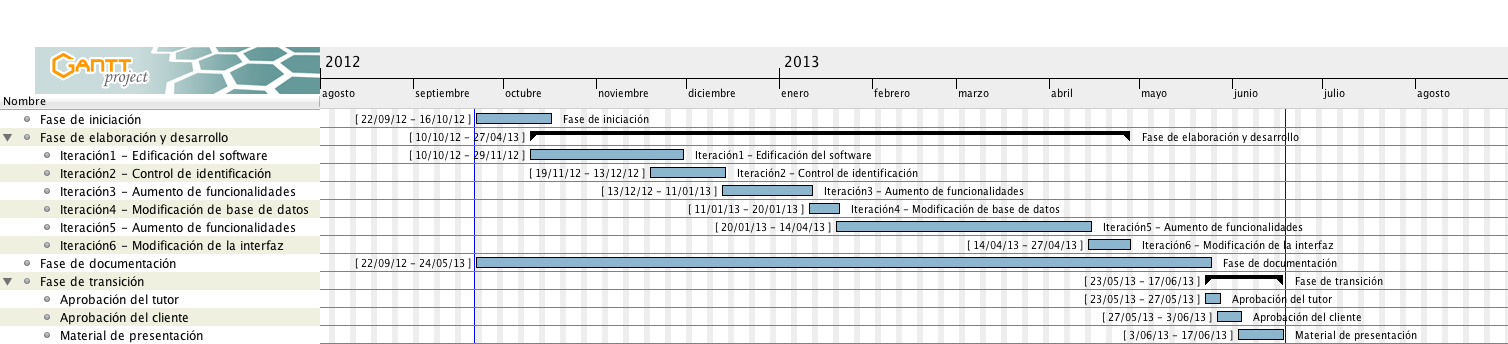
\includegraphics[angle=270,totalheight=22cm,width=8cm]{gantt}
  \caption{Diagrama de Gantt}
  \label{Figura}
\end{figure}

Se realizó la planificación de los tiempos de las tareas pero no se cumplieron debido a problemas no esperados o dificultad añadida no prevista.

\begin{table}[ht]
\centering  % used for centering table
\begin{tabular}{c c c} % centered columns (4 columns)
\hline\hline                        %inserts double horizontal lines
Fase & Tiempo estimado & Tiempo real \\ [0.5ex] % inserts table 
%heading
\hline                  % inserts single horizontal line
Fase de iniciación & 60 horas & 75 horas  \\ % inserting body of the table
Fase de elaboración y construcción & 400 horas & 550 horas \\
Fase de documentación & 30 horas &  50 horas\\
Fase de transición & 50 horas & 70 horas  \\ [1ex]      % [1ex] adds vertical space
\hline %inserts single line
\end{tabular}
\caption{Tiempo estimado - Tiempo real} % title of Table
\end{table}

\section{Organización}
Las personas involucradas en el proyecto son el tutor, el cliente y el desarrollador de la aplicación. El cliente es el que establece cuales son los requisitos y necesidades que quiere para su software mientras que el tutor es el que supervisa progresivamente que llevamos a cabo de forma correcta el proyecto.\\
Los recursos utilizados en el proyecto son un ordenador personal en el entorno de desarrollo y un servidor web donde alojaremos la aplicación. Todo el software usado es software libre por lo tanto no cabe destacar ningún coste salvo el tiempo empleado en desarrollar la aplicación.

\section{Costes}
\begin{itemize}
\item Costes humanos:
\end{itemize}
Para el cálculo de los costes humanos, se han utilizado las tablas salariales para figuras de personal investigador, contratado para el desarrollo de 
proyectos de investigación científica o técnica a través del contrato por obra y servicio aprobadas en 2012. En el documento alojado en la web\footnote{\url{http://www.uca.es/recursos/doc/Unidades/Area_Personal/Capitulo_VI/1143959322_942012113011.pdf}. \textit{Tablas salariales}}, se puede ver como el coste total anual de un ingeniero técnico son 23.237,88 y si calculamos la proporción por el tiempo de duración del proyecto que han sido 745 horas, aproximadamente 5 meses de dedicación el cual tiene un coste de 9.682,45 euros.
\begin{itemize}
\item Costes de materiales:
\end{itemize}
Todas las herramientas que se han usado e instalado son gratuitas y están instaladas en un sistema operativo Ubuntu 12.04.2 LTS, es decir, tanto el software utilizado como el sistema operativo son software libre y por lo tanto no representan ningún coste.

\newpage
\section{Gestión de riesgos}
La Gestión de riesgos es un enfoque estructurado para manejar la incertidumbre relativa a una amenaza, a través de una secuencia de actividades humanas que incluyen evaluación de riesgos, estrategias de desarrollo para manejarlo y mitigación del riesgo.\\
En esta sección describiremos mediante una tabla los riesgos del proyecto %\ref{Riesgos}:
\\
\begin{table}[ht]
\centering  % used for centering table
\begin{tabular}{c c c} % centered columns (4 columns)
\hline\hline                        %inserts double horizontal lines
Riesgo & Probabilidad & Impacto \\ [0.5ex] % inserts table 
%heading
\hline                  % inserts single horizontal line
Tiempo estimado demasiado pequeño & 70\% & 1 semana  \\ % inserting body of the table
Cliente cambia requisitos & 50\% & 1 semana \\
Falta experiencia en herramientas & 60\% & 2 semanas \\
Falta experiencia en planificación & 70\% & 1 semana \\
Falta experiencia en óptica & 80\% & 2 semanas  \\ [1ex]      % [1ex] adds vertical space
\hline %inserts single line
\end{tabular}
\label{Riesgos} % is used to refer this table in the text
\caption{Riesgos} % title of Table
\end{table}

Para disminuir los riesgos se tomaron varias citas con el cliente para definir bien los requisitos, se intentó tener buena experiencia en las herramientas para no entrar en los riesgos y se intentó hacer una buena planificación de los tiempos de las tareas.\\
El tiempo de la tarea aumentaría con cualquiera de los riesgos anteriormente citados.


% DESARROLLO
%\part{Desarrollo}
%\null\vfill
%\noindent En esta parte se debe describir el desarrollo del proyecto siguiendo la metodología empleada. Sus capítulos no deben ser una descripción exhaustiva de todos los documentos, diagramas, código fuente y, en general, entregables generados, sino más bien una explicación resumida del desarrollo, estructurada según las etapas principales del proceso de ingeniería. Deben seleccionarse aquellos diagramas, fragmentos de código y secciones de los entregables que sean más significativos para dicha explicación. La totalidad de los entregables resultado del proyecto se ubicarán en los anexos y/o en el material en CD/DVD que acompañe al proyecto.


\chapter{Análisis de Requisitos}
% ------------------------------------------------------------------------------
% Este fichero es parte de la plantilla LaTeX para la realización de Proyectos
% Final de Grado, protegido bajo los términos de la licencia GFDL.
% Para más información, la licencia completa viene incluida en el
% fichero fdl-1.3.tex

% Copyright (C) 2012 SPI-FM. Universidad de Cádiz
% ------------------------------------------------------------------------------

En esta sección se presenta el catálogo de requisitos del sistema de información. Para ello se detallarán los actores del sistema, los requisitos funcionales, los requisitos de información, los requisitos no funcionales, las reglas de negocio y las diferentes alternativas tecnológicas.
\section{Catálogo de actores}
Un Rol es una clasificación mediante la cual se definen distintos privilegios de operación para los usuarios del sistema. Los Roles se encuentran predefinidos en el sistema y se detallan a continuación:
\begin{itemize}
\item \textbf{Rol Empleado:} Son los usuarios normales de la aplicación, ellos pueden hacer uso de todo el sistema exceptuando las funciones propias del administrador y de los médicos.
\end{itemize}
\begin{itemize}
\item \textbf{Rol Médico:} Son usuarios de la aplicación con el rol empleado pero sólo ellos pueden crear informes de los clientes.
\end{itemize}
\begin{itemize}
\item \textbf{Rol Administrador:} Es el usuario del sistema con más privilegios. Puede realizar las funciones de un empleado pero con este rol pueden hacer algunas tareas propias de un administrador. No puede realizar informes.
\end{itemize}

\section{Requisitos funcionales}
A continuación se detallan, a partir del informe de necesidades de las entrevistas con el cliente, los requisitos funcionales de la aplicación:
\\
\begin{itemize}\renewcommand{\labelitemi}{$\diamond$}

\item Se debe disponer del control de usuarios del sistema con una pantalla de logueo, almacenando tanto la entrada como la salida del sistema.
\item Se debe tener un control de los roles de los usuarios del sistema.
\item Se debe tener una organización de los artículos del sistema agrupados por familias.
\item Se debe poder consultar el stock de los productos tanto stock reservado,apartado como stock real.
\item Se debe poder crear documentos con el logotipo de la empresa para opcionalmente su posterior impresión. 
\item Se debe poder crear documentos estadísticos para poder comparar datos.
\item Se debe tener un control de los usuarios del sistema.
\item Se debe tener un control de los proveedores del sistema.
\item Se debe tener un control de las citas que se generen.
\item Se debe tener un control de las reservas y apartados que generen los usuarios.
\item Se debe tener control de las devoluciones de los productos.
\item Se debe tener un control de las ventas realizadas a los clientes.
\item Se debe tener un control de los informes que se generen.
\item Se debe tener un control de los pedidos a los proveedores del sistema.
\item Se debe tener un control de los cambios realizados en el sistema.
\item Se debe tener un control de los arqueos realizados en el sistema.
\item Se debe tener un control de los permisos disfrutados por los usuarios de la aplicación.

\end{itemize}

\subsection{Requisito funcional: Gestión clientes}

\begin{itemize}
 \item El usuario podrá dar de alta a un determinado cliente. El cliente se identificará por su DNI. 
 \item El usuario podrá consultar e imprimir el listado de todos los clientes almacenados en el sistema.
 \item El usuario podrá ver los datos de un cliente en concreto.
 \item El usuario podrá modificar los datos de un cliente en concreto.
 \item El usuario podrá dar de baja a un cliente del sistema.
 \item El usuario podrá realizar filtrados de los clientes.
\end{itemize}


\begin{figure}[H]
  \centering
    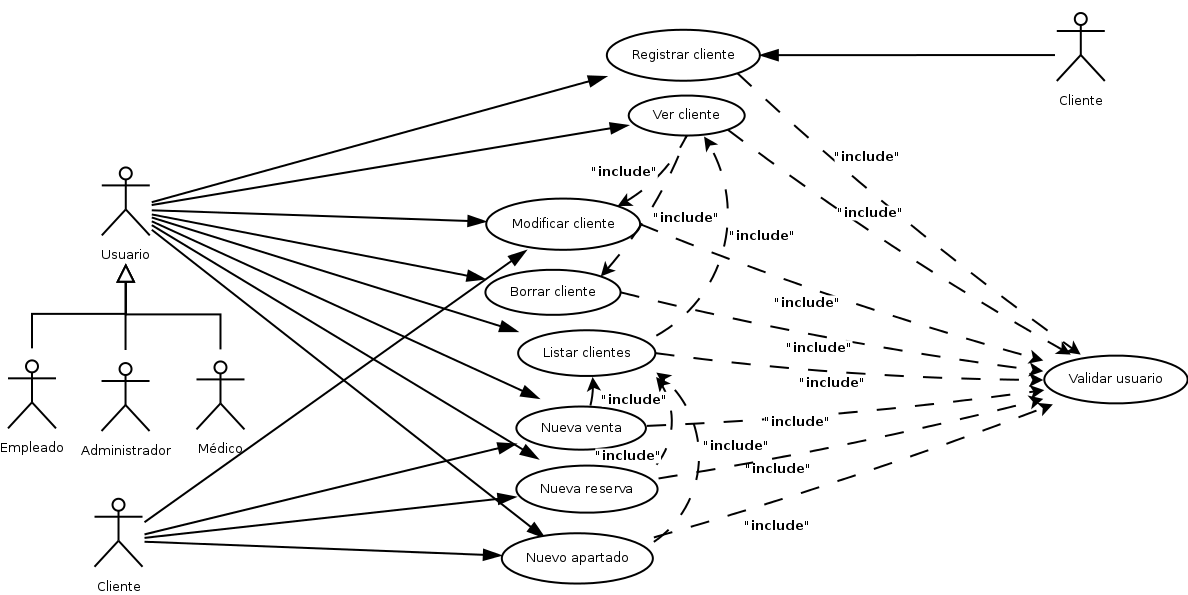
\includegraphics[scale=0.4]{gestionclientes.png}
  \caption{Diagrama caso de uso. Gestión de clientes}
  \label{cu1}
\end{figure}
\smallskip
\hrule height 1pt
\smallskip
\textbf{Caso de uso: Registrar cliente}
\begin{itemize}\renewcommand{\labelitemi}{$\cdot$}
 \item \textbf{Descripción:} El usuario introduce los datos para registrar un nuevo cliente en el sistema.
  \item \textbf{Actores:} Usuario(Principal), Cliente(Secundario)
  \item \textbf{Precondiciones:} Se debe comprobar que el usuario este autenticado en el sistema con el caso de uso Validar usuario.
  \item \textbf{Postcondiciones:} El sistema almacena al nuevo cliente en el sistema.
\end{itemize}
\underline{\textbf{Identificación de escenarios:}}
\begin{itemize}\renewcommand{\labelitemi}{$\circ$}
 \item \textbf{Escenario principal:}
         \begin{enumerate}
          \item El caso de uso se inicia cuando el usuario decide dar de alta un nuevo cliente.
          \item El usuario introduce los datos personales del cliente.
          \item El sistema muestra un mensaje de confirmación.
          \item El usuario pulsa SI en el mensaje de confirmación.
          \item El sistema comprueba que los datos introducidos son correctos y que el cliente no este registrado ya.
	  \item El sistema almacena el cambio del sistema (auditoria).
          \item El cliente queda registrado en el sistema y el sistema muestra un mensaje de éxito.
         \end{enumerate}
  \item \textbf{Escenario alternativos:}\\\\
         4a. El usuario cancela el registro de un nuevo cliente en el sistema.
	      \begin{enumerate}
	       \item El sistema cancela el registro de nuevo cliente en el sistema.
	      \end{enumerate}
	5a. El cliente ya se encuentra registrado en el sistema.
	      \begin{enumerate}
	       \item El sistema muestra el error y pide que se introduzcan nuevos datos.
	      \end{enumerate}
           5b. El usuario introduce de manera incorrecta los datos.
		\begin{enumerate}
		 \item El sistema muestra el error y pide que se introduzcan nuevos datos.
		\end{enumerate}
          *a. El usuario cancela el registro de un nuevo cliente.
\end{itemize}
\smallskip
\hrule height 1pt
\smallskip
\textbf{Caso de uso: Modificar cliente}
\begin{itemize}\renewcommand{\labelitemi}{$\cdot$}
 \item \textbf{Descripción:} El usuario modifica los datos del cliente en el sistema.
  \item \textbf{Actores:} Usuario(Principal), Cliente(Secundario)
  \item \textbf{Precondiciones:} El cliente ya existe en el sistema. Se debe comprobar que el usuario este autenticado en el sistema con el caso de uso Validar usuario.
  \item \textbf{Postcondiciones:} El sistema almacena al cliente con las modificaciones realizadas.
\end{itemize}
\underline{\textbf{Identificación de escenarios:}}
\begin{itemize}\renewcommand{\labelitemi}{$\circ$}
 \item \textbf{Escenario principal:}
         \begin{enumerate}
          \item El caso de uso se inicia cuando el usuario decide modificar un cliente.
          \item El usuario modifica los datos.
          \item El sistema muestra un mensaje de confirmación.
          \item El usuario pulsa SI en el mensaje de confirmación.
	  \item El sistema comprueba los datos introducidos por el usuario.
 	  \item El sistema almacena el cambio del sistema (auditoria).
          \item El sistema guarda los cambios que ha realizado el usuario.
       \end{enumerate}
  \item \textbf{Escenario alternativos:}\\\\
	4a. El usuario cancela la modificación del cliente en el sistema.
	      \begin{enumerate}
	       \item El sistema cancela la modificación del cliente en el sistema.
	      \end{enumerate}
           5a. El usuario modifica de manera incorrecta los datos.
		\begin{enumerate}
		 \item El sistema muestra el error y pide que se introduzcan nuevos datos.
		\end{enumerate}
          *a. El usuario cancela en cualquier momento la modificación de un cliente.
\end{itemize}
\smallskip
\hrule height 1pt
\smallskip
\textbf{Caso de uso: Borrar cliente}
\begin{itemize}\renewcommand{\labelitemi}{$\cdot$}
 \item \textbf{Descripción:} El usuario elimina a un cliente en el sistema.
  \item \textbf{Actores:} Usuario
  \item \textbf{Precondiciones:} El cliente ya existe en el sistema y no tiene operaciones asociadas. Se debe comprobar que el usuario este autenticado en el sistema con el caso de uso Validar usuario.
  \item \textbf{Postcondiciones:} El sistema borra el cliente del sistema.
\end{itemize}
\underline{\textbf{Identificación de escenarios:}}
\begin{itemize}\renewcommand{\labelitemi}{$\circ$}
 \item \textbf{Escenario principal:}
         \begin{enumerate}
          \item El caso de uso se inicia cuando el usuario decide borrar a un cliente.
          \item El sistema muestra un mensaje de confirmación.
          \item El usuario pulsa SI en el mensaje de confirmación.
 	  \item El sistema almacena el cambio del sistema (auditoria).
	  \item El sistema borra al cliente del sistema y muestra un mensaje de éxito.
         \end{enumerate}
  \item \textbf{Escenario alternativos:}\\\\
           3a. El usuario decide no borrar al cliente.
		\begin{enumerate}
		 \item El sistema cancela el proceso de borrado del cliente.
		\end{enumerate}
          *a. El usuario cancela en cualquier momento la eliminación de un cliente.
\end{itemize}

\smallskip
\hrule height 1pt
\smallskip

\textbf{Caso de uso: Ver cliente}
\begin{itemize}\renewcommand{\labelitemi}{$\cdot$}
 \item \textbf{Descripción:} El usuario decide hacer una consulta de un cliente en el sistema.
  \item \textbf{Actores:} Usuario
  \item \textbf{Precondiciones:} El cliente ya existe en el sistema. Se debe comprobar que el usuario este autenticado en el sistema con el caso de uso Validar usuario.
  \item \textbf{Postcondiciones:} El sistema muestra la información del cliente.
\end{itemize}
\underline{\textbf{Identificación de escenarios:}}
\begin{itemize}\renewcommand{\labelitemi}{$\circ$}
 \item \textbf{Escenario principal:}
         \begin{enumerate}
          \item El caso de uso se inicia cuando el usuario decide consultar a un cliente.
	  \item El sistema muestra por pantalla los datos del cliente.
         \end{enumerate}
\end{itemize}
\smallskip
\hrule height 1pt
\smallskip
\textbf{Caso de uso: Listar clientes}
\begin{itemize}\renewcommand{\labelitemi}{$\cdot$}
 \item \textbf{Descripción:} El usuario decide consultar los clientes almacenados en el sistema.
  \item \textbf{Actores:} Usuario
  \item \textbf{Precondiciones:} Se debe comprobar que el usuario este autenticado en el sistema con el caso de uso Validar usuario.
  \item \textbf{Postcondiciones:} El sistema muestra por pantalla todos los clientes.
\end{itemize}
\underline{\textbf{Identificación de escenarios:}}
\begin{itemize}\renewcommand{\labelitemi}{$\circ$}
 \item \textbf{Escenario principal:}
         \begin{enumerate}
          \item El caso de uso se inicia cuando el usuario decide consultar los clientes.
          \item El sistema muestra un listado de los clientes.
          \item El usuario no selecciona un patrón de búsqueda.
          \item El sistema muestra todos los clientes.
         \end{enumerate}
  \item \textbf{Escenario alternativos:}\\
  			3a. El usuario introduce un patrón de búsqueda.
  			\begin{enumerate}
  			\item El sistema muestra los datos acordes a ese patrón de búsqueda.
  			\item El usuario puede seleccionar el patrón de búsqueda cuantas veces desee.
  			\end{enumerate}
          *a. El usuario cancela en cualquier momento la consulta de los clientes.
\end{itemize}

\subsection{Requisito funcional: Gestión productos}

\begin{itemize}
 \item El usuario podrá dar de alta a un determinado producto. 
 \item El usuario podrá consultar e imprimir el listado de todos los productos almacenados en el sistema.
 \item El usuario podrá ver los datos de un producto en concreto.
 \item El usuario podrá modificar los datos de un producto en concreto.
 \item El usuario podrá eliminar un producto del sistema.
 \item El usuario podrá realizar filtrados en los productos.
 \item El usuario podrá dar de alta una determinada familia.
 \item El usuario podrá consultar e imprimir el listado de todas las familias almacenadas en el sistema.
 \item El usuario podrá modificar los datos de una familia en concreto.
 \item El usuario podrá eliminar a una familia del sistema.
 \item El usuario podrá realizar filtrados en las familias.
 \item El usuario podrá realizar movimientos de los productos de una familia a otra.
\item EL usuario podrá ver los productos incluidos en una determinada familia.

\end{itemize}
\begin{figure}[H]
  \centering
    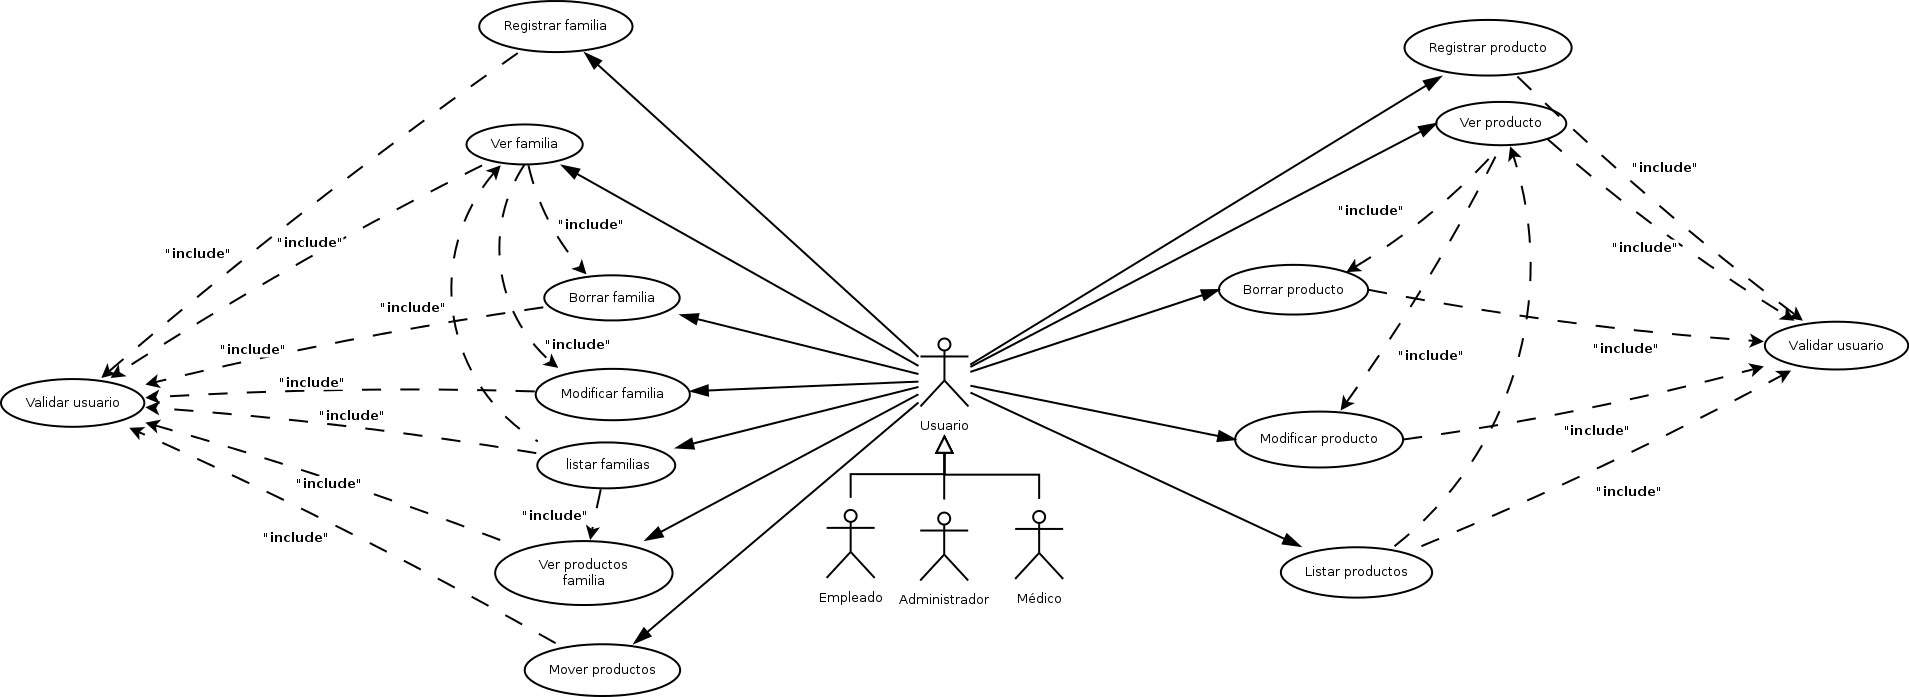
\includegraphics[width=17cm,height=8cm]{gestionproductos.png}
  \caption{Diagrama caso de uso. Gestión de productos}
  \label{cu2}
\end{figure}
\smallskip
\hrule height 1pt
\smallskip
\textbf{Caso de uso: Registrar producto}
\begin{itemize}\renewcommand{\labelitemi}{$\cdot$}
 \item \textbf{Descripción:} El usuario introduce los datos para registrar un nuevo producto en el sistema.
  \item \textbf{Actores:} Usuario
  \item \textbf{Precondiciones:} Se debe comprobar que el usuario este autenticado en el sistema con el caso de uso Validar usuario.
  \item \textbf{Postcondiciones:} El sistema almacena al producto en el sistema.
\end{itemize}
\underline{\textbf{Identificación de escenarios:}}
\begin{itemize}\renewcommand{\labelitemi}{$\circ$}
 \item \textbf{Escenario principal:}
         \begin{enumerate}
          \item El caso de uso se inicia cuando el usuario decide dar de alta un nuevo producto.
          \item El usuario introduce los datos del producto.
	   \item El sistema muestra un mensaje de confirmación.
          \item El usuario pulsa SI en el mensaje de confirmación.
          \item El sistema comprueba que los datos introducidos son correctos y que el producto no este registrado ya.
 	  \item El sistema almacena el cambio del sistema (auditoria).
          \item El producto queda registrado en el sistema y el sistema muestra un mensaje de éxito.
         \end{enumerate}
  \item \textbf{Escenario alternativos:}\\\\
	4a. El usuario decide no registrar un nuevo producto en el sistema.
	      \begin{enumerate}
	       \item El sistema cancela el registro del producto.
	      \end{enumerate}
         5a. El producto ya se encuentra registrado en el sistema.
	      \begin{enumerate}
	       \item El sistema muestra el error y pide que se introduzcan nuevos datos.
	      \end{enumerate}
           5b. El usuario introduce de manera incorrecta los datos.
		\begin{enumerate}
		 \item El sistema muestra el error y pide que se introduzcan nuevos datos.
		\end{enumerate}
          *a. El usuario cancela el registro de un nuevo producto.
\end{itemize}
\smallskip
\hrule height 1pt
\smallskip
\textbf{Caso de uso: Modificar producto}
\begin{itemize}\renewcommand{\labelitemi}{$\cdot$}
 \item \textbf{Descripción:} El usuario modifica los datos de un producto en el sistema.
  \item \textbf{Actores:} Usuario
  \item \textbf{Precondiciones:} El producto ya existe en el sistema. Se debe comprobar que el usuario este autenticado en el sistema con el caso de uso Validar usuario.
  \item \textbf{Postcondiciones:} El usuario almacena el producto con las modificaciones efectuadas en el sistema.
\end{itemize}
\underline{\textbf{Identificación de escenarios:}}
\begin{itemize}\renewcommand{\labelitemi}{$\circ$}
 \item \textbf{Escenario principal:}
         \begin{enumerate}
          \item El caso de uso se inicia cuando el usuario decide modificar un producto.
          \item El usuario modifica los datos del producto.
	  \item El sistema muestra un mensaje de confirmación.
          \item El usuario pulsa SI en el mensaje de confirmación.
          \item El sistema comprueba que los datos introducidos son correctos.
 	  \item El sistema almacena el cambio del sistema (auditoria).
          \item El sistema guarda los cambios que ha realizado el usuario.
         \end{enumerate}
  \item \textbf{Escenario alternativos:}\\\\
	4a. El usuario decide no modificar el producto del sistema.
	      \begin{enumerate}
	       \item El sistema cancela la edición del producto del sistema.
	      \end{enumerate}
           5a. El usuario modifica de manera incorrecta los datos.
		\begin{enumerate}
		 \item El sistema muestra el error y pide que se introduzcan nuevos datos.
		\end{enumerate}
          *a. El usuario cancela en cualquier momento la modificación de un producto.
\end{itemize}
\smallskip
\hrule height 1pt
\smallskip
\textbf{Caso de uso: Borrar producto}
\begin{itemize}\renewcommand{\labelitemi}{$\cdot$}
 \item \textbf{Descripción:} El usuario elimina a un producto en el sistema.
  \item \textbf{Actores:} Usuario
  \item \textbf{Precondiciones:} El producto ya existe en el sistema y no tiene operaciones asociadas. Se debe comprobar que el usuario este autenticado en el sistema con el caso de uso Validar usuario.
  \item \textbf{Postcondiciones:} El sistema borra el producto del sistema.
\end{itemize}
\underline{\textbf{Identificación de escenarios:}}
\begin{itemize}\renewcommand{\labelitemi}{$\circ$}
 \item \textbf{Escenario principal:}
         \begin{enumerate}
          \item El caso de uso se inicia cuando el usuario decide borrar a un producto.
          \item El sistema muestra un mensaje de confirmación.
          \item El usuario pulsa SI en el mensaje de confirmación.
 	  \item El sistema almacena el cambio del sistema (auditoria).
	  \item El sistema borra al producto del sistema y muestra un mensaje de éxito.
         \end{enumerate}
  \item \textbf{Escenario alternativos:}\\\\
           3a. El usuario decide no borrar el producto.
		\begin{enumerate}
		 \item El sistema cancela el proceso de borrado del producto.
		\end{enumerate}
          *a. El usuario cancela en cualquier momento la eliminación de un producto.
\end{itemize}
\smallskip
\hrule height 1pt
\smallskip

\textbf{Caso de uso: Ver producto}
\begin{itemize}\renewcommand{\labelitemi}{$\cdot$}
 \item \textbf{Descripción:} El usuario decide hacer una consulta de un producto en el sistema.
  \item \textbf{Actores:} Usuario
  \item \textbf{Precondiciones:} El producto ya existe en el sistema. Se debe comprobar que el usuario este autenticado en el sistema con el caso de uso Validar usuario.
  \item \textbf{Postcondiciones:} El sistema muestra la información del producto.
\end{itemize}
\underline{\textbf{Identificación de escenarios:}}
\begin{itemize}\renewcommand{\labelitemi}{$\circ$}
 \item \textbf{Escenario principal:}
         \begin{enumerate}
          \item El caso de uso se inicia cuando el usuario decide consultar a un producto del sistema.
	  \item El sistema muestra por pantalla los datos del producto.
         \end{enumerate}
  \item \textbf{Escenario alternativos:}\\\\
          *a. El usuario cancela en cualquier momento la consulta de un producto.
\end{itemize}
\smallskip
\hrule height 1pt
\smallskip
\textbf{Caso de uso: Listar productos}
\begin{itemize}\renewcommand{\labelitemi}{$\cdot$}
 \item \textbf{Descripción:} El usuario consulta los productos almacenados en el sistema.
  \item \textbf{Actores:} usuario
  \item \textbf{Precondiciones:} En el sistema existe al menos un producto. Se debe comprobar que el usuario este autenticado en el sistema con el caso de uso Validar usuario.
  \item \textbf{Postcondiciones:} El sistema muestra por pantalla todos los productos almacenados en el sistema.
\end{itemize}
\underline{\textbf{Identificación de escenarios:}}
\begin{itemize}\renewcommand{\labelitemi}{$\circ$}
 \item \textbf{Escenario principal:}
         \begin{enumerate}
          \item El caso de uso se inicia cuando el usuario decide consultar los productos.
          \item El sistema muestra un listado de los productos.
          \item El usuario no selecciona un patrón de búsqueda.
          \item El sistema muestra todos los productos.
         \end{enumerate}
  \item \textbf{Escenario alternativos:}\\
  			3a. El usuario introduce un patrón de búsqueda.
  			\begin{enumerate}
  			\item El sistema muestra los datos acordes a ese patrón de búsqueda.
  			\item El usuario puede seleccionar el patrón de búsqueda cuantas veces desee.
  			\end{enumerate}
          *a. El usuario cancela en cualquier momento la consulta de los productos.
\end{itemize}
\smallskip
\hrule height 1pt
\smallskip
\textbf{Caso de uso: Registrar familia}
\begin{itemize}\renewcommand{\labelitemi}{$\cdot$}
 \item \textbf{Descripción:} El usuario introduce los datos para registrar una nueva familia en el sistema.
  \item \textbf{Actores:} Usuario
  \item \textbf{Precondiciones:} Se debe comprobar que el usuario este autenticado en el sistema con el caso de uso Validar usuario.
  \item \textbf{Postcondiciones:} El usuario almacena la familia en el sistema.
\end{itemize}
\underline{\textbf{Identificación de escenarios:}}
\begin{itemize}\renewcommand{\labelitemi}{$\circ$}
 \item \textbf{Escenario principal:}
         \begin{enumerate}
          \item El caso de uso se inicia cuando el usuario decide dar de alta una nueva familia.
          \item El usuario introduce los datos de la familia.
	  \item El sistema muestra un mensaje de confirmación.
          \item El usuario pulsa SI en el mensaje de confirmación.
          \item El sistema comprueba que los datos introducidos son correctos y que la familia no este registrada ya.
 	  \item El sistema almacena el cambio del sistema (auditoria).
          \item La familia queda registrada en el sistema y el sistema muestra un mensaje de éxito.
         \end{enumerate}
  \item \textbf{Escenario alternativos:}\\\\
	4a. El usuario decide no registrar una nueva familia en el sistema.
	      \begin{enumerate}
	       \item El sistema cancela el registro de una nueva familia en el sistema.
	      \end{enumerate}
         5a. La familia ya se encuentra registrada en el sistema.
	      \begin{enumerate}
	       \item El sistema muestra el error y pide que se introduzcan nuevos datos.
	      \end{enumerate}
           5b. El usuario introduce de manera incorrecta los datos.
		\begin{enumerate}
		 \item El sistema muestra el error y pide que se introduzcan nuevos datos.
		\end{enumerate}
         *a. El usuario cancela el registro de una nueva familia.
\end{itemize}
\smallskip
\hrule height 1pt
\smallskip
\textbf{Caso de uso: Modificar familia}
\begin{itemize}\renewcommand{\labelitemi}{$\cdot$}
 \item \textbf{Descripción:} El usuario modifica los datos de una familia.
  \item \textbf{Actores:} Usuario
  \item \textbf{Precondiciones:} La familia ya existe en el sistema. Se debe comprobar que el usuario este autenticado en el sistema con el caso de uso Validar usuario.
  \item \textbf{Postcondiciones:} El usuario almacena la familia con las modificaciones efectuadas en el sistema.
\end{itemize}
\underline{\textbf{Identificación de escenarios:}}
\begin{itemize}\renewcommand{\labelitemi}{$\circ$}
 \item \textbf{Escenario principal:}
         \begin{enumerate}
          \item El caso de uso se inicia cuando el usuario decide modificar una familia.
          \item El usuario modifica los datos de la familia.
	  \item El sistema muestra un mensaje de confirmación.
          \item El usuario pulsa SI en el mensaje de confirmación.
          \item El sistema comprueba que los datos introducidos sean correctos.
 	  \item El sistema almacena el cambio del sistema (auditoria).
          \item El sistema guarda los cambios que ha realizado el usuario.
         \end{enumerate}
  \item \textbf{Escenario alternativos:}\\\\	
	4a. El usuario decide no modificar la familia del sistema.
	      \begin{enumerate}
	       \item El sistema cancela la edición de la familia en el sistema.
	      \end{enumerate}
           5a. El usuario modifica de manera incorrecta los datos.
		\begin{enumerate}
		 \item El sistema muestra el error y pide que se introduzcan nuevos datos.
		\end{enumerate}
          *a. El usuario cancela en cualquier momento la modificación de una familia.
\end{itemize}
\smallskip
\hrule height 1pt
\smallskip
\textbf{Caso de uso: Borrar familia}
\begin{itemize}\renewcommand{\labelitemi}{$\cdot$}
 \item \textbf{Descripción:} El usuario elimina a una familia en el sistema.
  \item \textbf{Actores:} usuario
  \item \textbf{Precondiciones:} La familia ya existe en el sistema. Se debe comprobar que el usuario este autenticado en el sistema con el caso de uso Validar usuario.
  \item \textbf{Postcondiciones:} El sistema borra la familia del sistema.
\end{itemize}
\underline{\textbf{Identificación de escenarios:}}
\begin{itemize}\renewcommand{\labelitemi}{$\circ$}
 \item \textbf{Escenario principal:}
         \begin{enumerate}
          \item El caso de uso se inicia cuando el usuario decide borrar a una familia.
          \item El sistema muestra un mensaje de confirmación.
          \item El usuario pulsa SI en el mensaje de confirmación.
 	  \item El sistema almacena el cambio del sistema (auditoria).
	   \item El sistema deja los productos sin familia, se borra la familia del sistema y muestra un mensaje de éxito.
         \end{enumerate}
  \item \textbf{Escenario alternativos:}\\\\
	3a. El usuario decide no borrar la familia.
		\begin{enumerate}
		 \item El sistema cancela el proceso de borrado de la familia.
		\end{enumerate}
          *a. El usuario cancela en cualquier momento la eliminación de la familia.
\end{itemize}

\smallskip
\hrule height 1pt
\smallskip
\textbf{Caso de uso: Ver familia}
\begin{itemize}\renewcommand{\labelitemi}{$\cdot$}
 \item \textbf{Descripción:} El usuario decide hacer una consulta de una familia en el sistema.
  \item \textbf{Actores:} usuario
  \item \textbf{Precondiciones:} La familia ya existe en el sistema. Se debe comprobar que el usuario este autenticado en el sistema con el caso de uso Validar usuario.
  \item \textbf{Postcondiciones:} El sistema muestra la información de la familia por pantalla.
\end{itemize}
\underline{\textbf{Identificación de escenarios:}}
\begin{itemize}\renewcommand{\labelitemi}{$\circ$}
 \item \textbf{Escenario principal:}
         \begin{enumerate}
          \item El caso de uso se inicia cuando el usuario decide consultar a una familia del sistema.
	  \item El sistema muestra por pantalla los datos de la familia.
         \end{enumerate}
  \item \textbf{Escenario alternativos:}\\\\
          *a. El usuario cancela en cualquier momento la consulta de una familia.
\end{itemize}
\smallskip
\hrule height 1pt
\smallskip
\textbf{Caso de uso: Listar familias}
\begin{itemize}\renewcommand{\labelitemi}{$\cdot$}
 \item \textbf{Descripción:} El usuario consulta las familias almacenadas en el sistema.
  \item \textbf{Actores:} usuario
  \item \textbf{Precondiciones:} En el sistema existe al menos una familia. Se debe comprobar que el usuario este autenticado en el sistema con el caso de uso Validar usuario.
  \item \textbf{Postcondiciones:} El sistema muestra por pantalla todas las familias almacenadas en el sistema.
\end{itemize}
\underline{\textbf{Identificación de escenarios:}}
\begin{itemize}\renewcommand{\labelitemi}{$\circ$}
 \item \textbf{Escenario principal:}
         \begin{enumerate}
          \item El caso de uso se inicia cuando el usuario decide consultar las familias.
          \item El sistema muestra un listado de las familias.
          \item El usuario no selecciona un patrón de búsqueda.
          \item El sistema muestra todas las familias.
         \end{enumerate}
  \item \textbf{Escenario alternativos:}\\
  			3a. El usuario introduce un patrón de búsqueda.
  			\begin{enumerate}
  			\item El sistema muestra los datos acordes a ese patrón de búsqueda.
  			\item El usuario puede seleccionar el patrón de búsqueda cuantas veces desee.
  			\end{enumerate}
          *a. El usuario cancela en cualquier momento la consulta de las familias.
\end{itemize}
\smallskip
\hrule height 1pt
\smallskip
\textbf{Caso de uso: Mover productos}
\begin{itemize}\renewcommand{\labelitemi}{$\cdot$}
 \item \textbf{Descripción:} El usuario mueve los productos entre las familias del sistema.
  \item \textbf{Actores:} Usuario
  \item \textbf{Precondiciones:} Se debe comprobar que el usuario este autenticado en el sistema con el caso de uso Validar usuario.
  \item \textbf{Postcondiciones:} El sistema cambia de familia a los productos deseados por el usuario.
\end{itemize}
\underline{\textbf{Identificación de escenarios:}}
\begin{itemize}\renewcommand{\labelitemi}{$\circ$}
 \item \textbf{Escenario principal:}
         \begin{enumerate}
          \item El caso de uso se inicia cuando el usuario decide mover productos.
          \item El sistema muestra dos cajas para poder mover productos entre familias.
          \item El usuario selecciona las familias afectadas.
          \item El usuario arrastra los productos de una familia a otra.
 	  \item El sistema almacena el cambio del sistema (auditoria).
          \item El sistema guarda los cambios.
         \end{enumerate}
  \item \textbf{Escenario alternativos:}\\
  	   3a. El usuario puede seleccionar las familias afectadas y productos cuantas veces desee.\\
           *a. El usuario cancela en cualquier momento el movimiento de productos.
\end{itemize}

\subsection{Requisito funcional: Gestión proveedores}

\begin{itemize}
 \item El usuario podrá dar de alta a un determinado proveedor. 
 \item El usuario podrá consultar e imprimir el listado de todos los proveedores almacenados en el sistema.
 \item El usuario podrá ver los datos de un proveedor en concreto.
 \item El usuario podrá modificar los datos de un proveedor en concreto.
 \item El usuario podrá eliminar a un proveedor del sistema.
 \item El usuario podrá realizar filtrados de los proveedores.
\item El usuario podrá ver los productos suministrados por un determinado proveedor.
\end{itemize}
\begin{figure}[H]
  \centering
    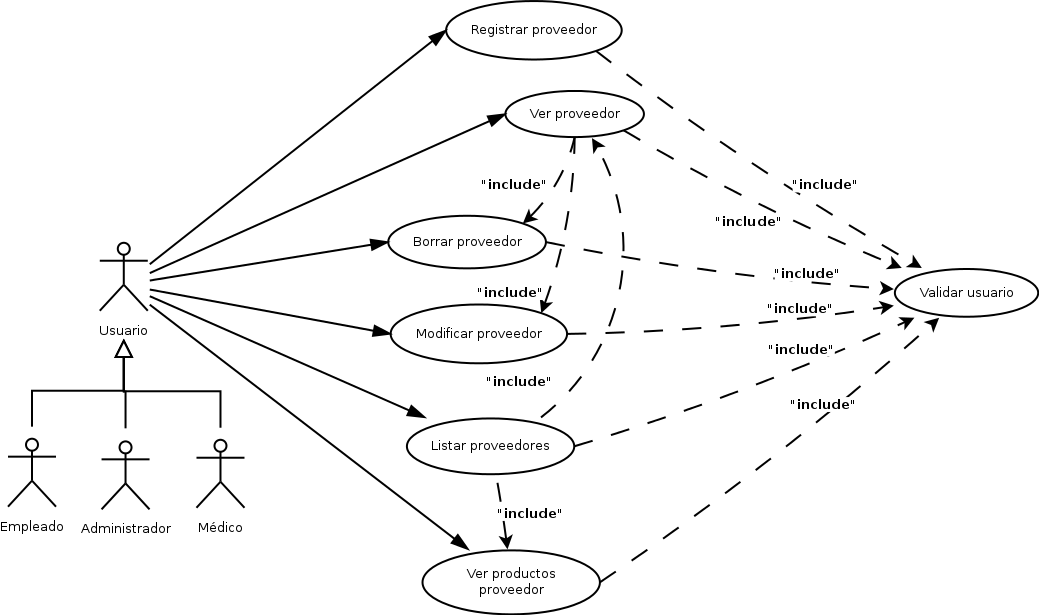
\includegraphics[width=12cm,height=8cm]{gestionproveedores.png}
  \caption{Diagrama caso de uso. Gestión de proveedores}
  \label{cu3}
\end{figure}
\smallskip
\hrule height 1pt
\smallskip
\textbf{Caso de uso: Registrar proveedor}
\begin{itemize}\renewcommand{\labelitemi}{$\cdot$}
 \item \textbf{Descripción:} El usuario introduce los datos para registrar un nuevo proveedor en el sistema.
  \item \textbf{Actores:} Usuario
  \item \textbf{Precondiciones:} Se debe comprobar que el usuario este autenticado en el sistema con el caso de uso Validar usuario.
  \item \textbf{Postcondiciones:} El usuario almacena al proveedor en el sistema.
\end{itemize}
\underline{\textbf{Identificación de escenarios:}}
\begin{itemize}\renewcommand{\labelitemi}{$\circ$}
 \item \textbf{Escenario principal:}
         \begin{enumerate}
          \item El caso de uso se inicia cuando el usuario decide dar de alta un nuevo proveedor.
          \item El usuario introduce los datos del proveedor.
          \item El sistema muestra un mensaje de confirmación.
          \item El usuario pulsa SI en el mensaje de confirmación.
          \item El sistema comprueba que los datos introducidos son correctos y que el proveedor no este registrado ya.
 	  \item El sistema almacena el cambio del sistema (auditoria).
          \item El proveedor queda registrado en el sistema y el sistema muestra un mensaje de éxito.
         \end{enumerate}
  \item \textbf{Escenario alternativos:}\\\\
	4a. El usuario decide no registrar un nuevo proveedor en el sistema.
	      \begin{enumerate}
	       \item El sistema cancela el registro de un nuevo proveedor en el sistema.
	      \end{enumerate}
         5a. El proveedor ya se encuentra registrado en el sistema.
	      \begin{enumerate}
	       \item El sistema muestra el error y pide que se introduzcan nuevos datos.
	      \end{enumerate}
           5b. El usuario introduce de manera incorrecta los datos.
		\begin{enumerate}
		 \item El sistema muestra el error y pide que se introduzcan nuevos datos.
		\end{enumerate}
          *a. El usuario cancela el registro de un nuevo proveedor.
\end{itemize}
\smallskip
\hrule height 1pt
\smallskip
\textbf{Caso de uso: Editar proveedor}
\begin{itemize}\renewcommand{\labelitemi}{$\cdot$}
 \item \textbf{Descripción:} El usuario modifica los datos del proveedor en el sistema.
  \item \textbf{Actores:} Usuario
  \item \textbf{Precondiciones:} El proveedor ya existe en el sistema. Se debe comprobar que el usuario este autenticado en el sistema con el caso de uso Validar usuario.
  \item \textbf{Postcondiciones:} El usuario almacena al proveedor con las modificaciones efectuadas en el sistema.
\end{itemize}
\underline{\textbf{Identificación de escenarios:}}
\begin{itemize}\renewcommand{\labelitemi}{$\circ$}
 \item \textbf{Escenario principal:}
         \begin{enumerate}
          \item El caso de uso se inicia cuando el usuario decide modificar un proveedor.
          \item El usuario modifica los datos.
          \item El sistema muestra un mensaje de confirmación.
          \item El usuario pulsa SI en el mensaje de confirmación.
          \item El sistema comprueba que los datos introducidos son correctos.
 	  \item El sistema almacena el cambio del sistema (auditoria).
          \item El sistema guarda los cambios que ha realizado el usuario.
         \end{enumerate}
  \item \textbf{Escenario alternativos:}\\\\
	4a. El usuario decide no editar al proveedor.
	      \begin{enumerate}
	       \item El sistema cancela la edición del proveedor en el sistema.
	      \end{enumerate}
           5a. El usuario modifica de manera incorrecta los datos.
		\begin{enumerate}
		 \item El sistema muestra el error y pide que se introduzcan nuevos datos.
		\end{enumerate}
          *a. El usuario cancela en cualquier momento la edición de un proveedor.
\end{itemize}
\smallskip
\hrule height 1pt
\smallskip
\textbf{Caso de uso: Borrar proveedor}
\begin{itemize}\renewcommand{\labelitemi}{$\cdot$}
 \item \textbf{Descripción:} El usuario elimina a un proveedor en el sistema.
  \item \textbf{Actores:} Usuario
  \item \textbf{Precondiciones:} El proveedor ya existe en el sistema. Se debe comprobar que el usuario este autenticado en el sistema con el caso de uso Validar usuario.
  \item \textbf{Postcondiciones:} El sistema borra al proveedor del sistema.
\end{itemize}
\underline{\textbf{Identificación de escenarios:}}
\begin{itemize}\renewcommand{\labelitemi}{$\circ$}
 \item \textbf{Escenario principal:}
         \begin{enumerate}
          \item El caso de uso se inicia cuando el usuario decide borrar a un proveedor.
          \item El sistema muestra un mensaje de confirmación.
          \item El usuario pulsa SI en el mensaje de confirmación.
 	  \item El sistema almacena el cambio del sistema (auditoria).
	      \item El sistema borra al proveedor del sistema y muestra un mensaje de éxito.
         \end{enumerate}
  \item \textbf{Escenario alternativos:}\\\\
           3a. El usuario decide no borrar al proveedor.
		\begin{enumerate}
		 \item El sistema cancela el proceso de borrado del proveedor.
		\end{enumerate}
          *a. El usuario cancela en cualquier momento la eliminación de un proveedor.
\end{itemize}
\smallskip
\hrule height 1pt
\smallskip

\textbf{Caso de uso: Ver proveedor}
\begin{itemize}\renewcommand{\labelitemi}{$\cdot$}
 \item \textbf{Descripción:} El usuario decide hacer una consulta de un proveedor en el sistema.
  \item \textbf{Actores:} usuario
  \item \textbf{Precondiciones:} El proveedor ya existe en el sistema. Se debe comprobar que el usuario este autenticado en el sistema con el caso de uso Validar usuario.
  \item \textbf{Postcondiciones:} El sistema muestra la información del proveedor.
\end{itemize}
\underline{\textbf{Identificación de escenarios:}}
\begin{itemize}\renewcommand{\labelitemi}{$\circ$}
 \item \textbf{Escenario principal:}
         \begin{enumerate}
          \item El caso de uso se inicia cuando el usuario decide consultar a un proveedor.
	  \item El sistema muestra por pantalla los datos del proveedor.
         \end{enumerate}
\end{itemize}
\smallskip
\hrule height 1pt
\smallskip
\textbf{Caso de uso: Listar proveedores}
\begin{itemize}\renewcommand{\labelitemi}{$\cdot$}
 \item \textbf{Descripción:} El usuario consulta los proveedores almacenados en el sistema.
  \item \textbf{Actores:} usuario
  \item \textbf{Precondiciones:} En el sistema existe al menos un proveedor. Se debe comprobar que el usuario este autenticado en el sistema con el caso de uso Validar usuario.
  \item \textbf{Postcondiciones:} El sistema muestra por pantalla todos los proveedores.
\end{itemize}
\underline{\textbf{Identificación de escenarios:}}
\begin{itemize}\renewcommand{\labelitemi}{$\circ$}
 \item \textbf{Escenario principal:}
         \begin{enumerate}
          \item El caso de uso se inicia cuando el usuario decide consultar los proveedores.
          \item El sistema muestra un listado de los proveedores.
          \item El usuario no selecciona un patrón de búsqueda.
          \item El sistema muestra todos los proveedores.
         \end{enumerate}
  \item \textbf{Escenario alternativos:}\\
  			3a. El usuario introduce un patrón de búsqueda.
  			\begin{enumerate}
  			\item El sistema muestra los datos acordes a ese patrón de búsqueda.
  			\item El usuario puede seleccionar el patrón de búsqueda cuantas veces desee.
  			\end{enumerate}
          *a. El usuario cancela en cualquier momento la consulta de los proveedores.
\end{itemize}

\subsection{Requisito funcional: Gestión usuarios}

\begin{itemize}
 \item El administrador podrá dar de alta a un determinado usuario. El usuario se identificará por su DNI. 
 \item El administrador podrá consultar e imprimir el listado de todos los usuarios almacenados en el sistema.
 \item El administrador podrá ver los datos de un usuario en concreto.
 \item El administrador podrá modificar los datos de un usuario en concreto.
 \item El administrador podrá desactivar a un usuario del sistema.
 \item El administrador podrá realizar filtrados de los usuarios del sistema.

\end{itemize}
\begin{figure}[H]
  \centering
    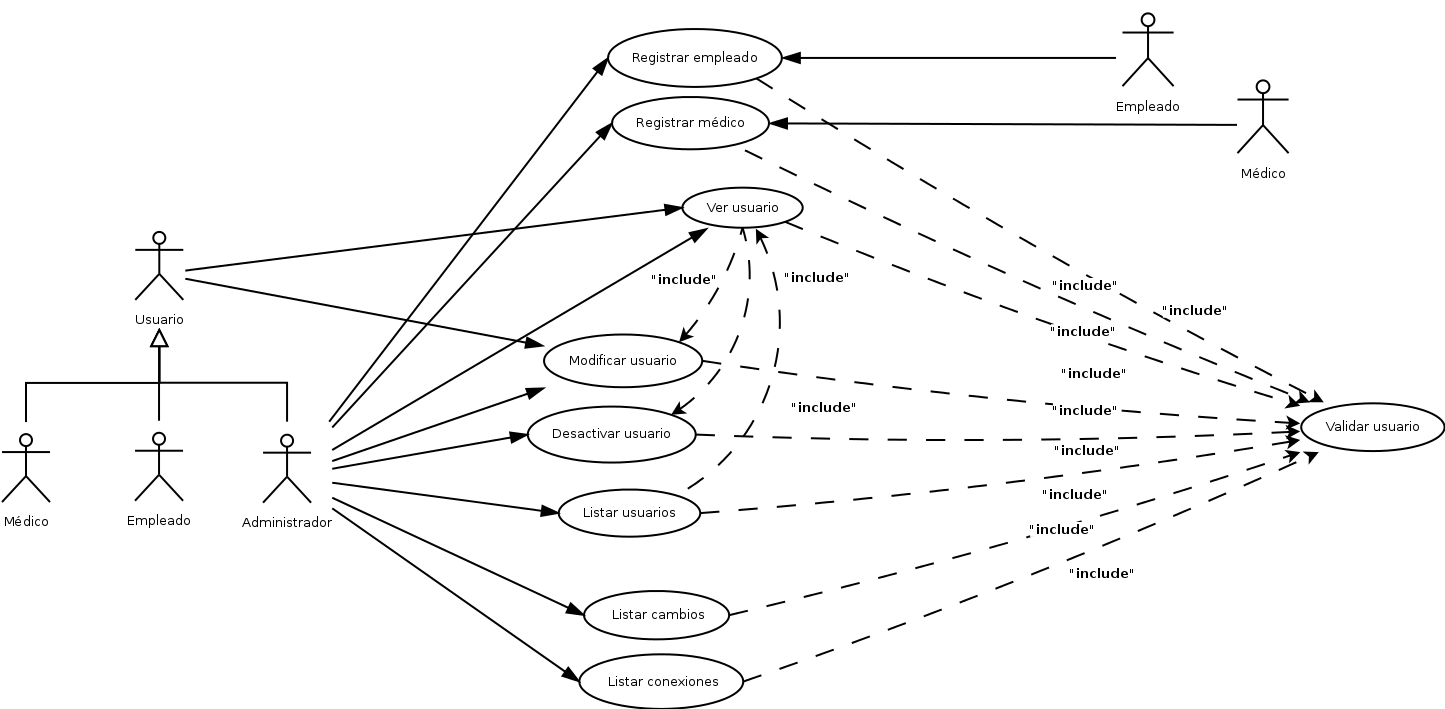
\includegraphics[width=12cm,height=8cm]{gestionempledos.png}
  \caption{Diagrama caso de uso. Gestión de usuarios}
  \label{cu4}
\end{figure}
\smallskip
\hrule height 1pt
\smallskip
\textbf{Caso de uso: Registrar empleado}
\begin{itemize}\renewcommand{\labelitemi}{$\cdot$}
 \item \textbf{Descripción:} El administrador introduce los datos para registrar un nuevo empleado en el sistema.
  \item \textbf{Actores:} Administrador
  \item \textbf{Precondiciones:} Se debe comprobar que el administrador este autenticado en el sistema con el caso de uso Validar usuario.
  \item \textbf{Postcondiciones:} El administrador almacena al empleado en el sistema.
\end{itemize}
\underline{\textbf{Identificación de escenarios:}}
\begin{itemize}\renewcommand{\labelitemi}{$\circ$}
 \item \textbf{Escenario principal:}
         \begin{enumerate}
          \item El caso de uso se inicia cuando el administrador decide dar de alta un nuevo empleado.
          \item El administrador introduce los datos del empleado.
  	  \item El sistema muestra un mensaje de confirmación.
          \item El administrador pulsa SI en el mensaje de confirmación.
          \item El sistema comprueba que los datos introducidos son correctos y que el empleado no este registrado ya.
       	  \item El sistema manda un email con la contraseña al nuevo empleado.
 	  \item El sistema almacena el cambio del sistema (auditoria).
          \item El empleado queda registrado en el sistema y el sistema muestra un mensaje de éxito.
         \end{enumerate}
  \item \textbf{Escenario alternativos:}\\\\
	4a. El administrador decide no registrar a un nuevo empleado.
	      \begin{enumerate}
	       \item El sistema cancela el registro de un nuevo empleado en el sistema.
	      \end{enumerate}
         5a. El empleado ya se encuentra registrado en el sistema.
	      \begin{enumerate}
	       \item El sistema muestra el error y pide que se introduzcan nuevos datos.
	      \end{enumerate}
           5b. El administrador introduce de manera incorrecta los datos.
		\begin{enumerate}
		 \item El sistema muestra el error y pide que se introduzcan nuevos datos.
		\end{enumerate}
          *a. El administrador cancela el registro de un nuevo empleado.
\end{itemize}
\smallskip
\hrule height 1pt
\smallskip
\textbf{Caso de uso: Registrar médico}
\begin{itemize}\renewcommand{\labelitemi}{$\cdot$}
 \item \textbf{Descripción:} El administrador introduce los datos para registrar un nuevo médico en el sistema.
  \item \textbf{Actores:} Administrador
  \item \textbf{Precondiciones:} Se debe comprobar que el administrador este autenticado en el sistema con el caso de uso Validar usuario.
  \item \textbf{Postcondiciones:} El administrador almacena al médico en el sistema.
\end{itemize}
\underline{\textbf{Identificación de escenarios:}}
\begin{itemize}\renewcommand{\labelitemi}{$\circ$}
 \item \textbf{Escenario principal:}
         \begin{enumerate}
          \item El caso de uso se inicia cuando el administrador decide dar de alta un nuevo médico.
          \item El usuario introduce los datos del médico.
  	  \item El sistema muestra un mensaje de confirmación.
          \item El administrador pulsa SI en el mensaje de confirmación.
          \item El sistema comprueba que los datos introducidos son correctos y que el médico no este registrado ya.
	\item El sistema manda un email con la contraseña al nuevo usuario.
 	  \item El sistema almacena el cambio del sistema (auditoria).
          \item El médico queda registrado en el sistema y el sistema muestra un mensaje de éxito.
         \end{enumerate}
  \item \textbf{Escenario alternativos:}\\\\
	4a. El administrador decide no registrar a un nuevo médico.
	      \begin{enumerate}
	       \item El sistema cancela el registro de un nuevo médico en el sistema.
	      \end{enumerate}
         5a. El médico ya se encuentra registrado en el sistema.
	      \begin{enumerate}
	       \item El sistema muestra el error y pide que se introduzcan nuevos datos.
	      \end{enumerate}
           5b. El administrador introduce de manera incorrecta los datos.
		\begin{enumerate}
		 \item El sistema muestra el error y pide que se introduzcan nuevos datos.
		\end{enumerate}
          *a. El administrador cancela el registro de un nuevo médico.
\end{itemize}
\smallskip
\hrule height 1pt
\smallskip
\textbf{Caso de uso: Modificar empleado}
\begin{itemize}\renewcommand{\labelitemi}{$\cdot$}
 \item \textbf{Descripción:} El administrador modifica los datos de un empleado en el sistema.
  \item \textbf{Actores:} Administrador, Usuario
  \item \textbf{Precondiciones:} El empleado ya existe en el sistema. Se debe comprobar que el administrador este autenticado en el sistema con el caso de uso Validar usuario. Si el usuario no es administrador sólo podrá modificar sus propios datos.
  \item \textbf{Postcondiciones:} El administrador almacena al empleado con las modificaciones efectuadas en el sistema.
\end{itemize}
\underline{\textbf{Identificación de escenarios:}}
\begin{itemize}\renewcommand{\labelitemi}{$\circ$}
 \item \textbf{Escenario principal:}
         \begin{enumerate}
          \item El caso de uso se inicia cuando el administrador decide modificar un empleado.
          \item El administrador modifica los datos.
  	  \item El sistema muestra un mensaje de confirmación.
          \item El usuario pulsa SI en el mensaje de confirmación.
          \item El sistema comprueba que los datos introducidos son correctos.
 	  \item El sistema almacena el cambio del sistema (auditoria).
          \item El sistema guarda los cambios que ha realizado el administrador.
         \end{enumerate}
  \item \textbf{Escenario alternativos:}\\\\
	   4a. El administrador decide no editar al empleado.
	      \begin{enumerate}
	       \item El sistema cancela la edición de un empleado en el sistema.
	      \end{enumerate}
           5a. El administrador modifica de manera incorrecta los datos.
		\begin{enumerate}
		 \item El sistema muestra el error y pide que se introduzcan nuevos datos.
		\end{enumerate}
          *a. El administrador cancela en cualquier momento la edición de un empleado.
\end{itemize}
\smallskip
\hrule height 1pt
\smallskip

\textbf{Caso de uso: Desactivar empleado}
\begin{itemize}\renewcommand{\labelitemi}{$\cdot$}
 \item \textbf{Descripción:} El administrador desactiva a un empleado en el sistema.
  \item \textbf{Actores:} Administrador
  \item \textbf{Precondiciones:} El empleado ya existe en el sistema. Se debe comprobar que el administrador este autenticado en el sistema con el caso de uso Validar usuario.
  \item \textbf{Postcondiciones:} El sistema desactiva al empleado del sistema.
\end{itemize}
\underline{\textbf{Identificación de escenarios:}}
\begin{itemize}\renewcommand{\labelitemi}{$\circ$}
 \item \textbf{Escenario principal:}
         \begin{enumerate}
          \item El caso de uso se inicia cuando el administrador decide desactivar a un empleado.
          \item El sistema muestra un mensaje de confirmación.
          \item El administrador pulsa SI en el mensaje de confirmación.
 	  \item El sistema almacena el cambio del sistema (auditoria).
	   \item El sistema desactiva al usuario del sistema y muestra un mensaje de éxito.
         \end{enumerate}
  \item \textbf{Escenario alternativos:}\\\\
           3a. El administrador decide no desactivar al usuario.
		\begin{enumerate}
		 \item El sistema cancela el proceso de desactivación del usuario.
		\end{enumerate}
          *a. El administrador cancela en cualquier momento la desactivación de un usuario.
\end{itemize}
\smallskip
\hrule height 1pt
\smallskip
\textbf{Caso de uso: Ver empleado}
\begin{itemize}\renewcommand{\labelitemi}{$\cdot$}
 \item \textbf{Descripción:} El administrador decide hacer una consulta de un empleado en el sistema.
  \item \textbf{Actores:} Administrador, Usuario
  \item \textbf{Precondiciones:} El empleado ya existe en el sistema. Se debe comprobar que el empleado este autenticado en el sistema con el caso de uso Validar usuario. Si el usuario no es administrador sólo podrá ver sus propios datos.
  \item \textbf{Postcondiciones:} El sistema muestra la información del empleado.
\end{itemize}
\underline{\textbf{Identificación de escenarios:}}
\begin{itemize}\renewcommand{\labelitemi}{$\circ$}
 \item \textbf{Escenario principal:}
         \begin{enumerate}
          \item El caso de uso se inicia cuando el administrador decide consultar a un empleado.
	  \item El sistema muestra por pantalla los datos del empleado.
         \end{enumerate}
\end{itemize}
\smallskip
\hrule height 1pt
\smallskip
\textbf{Caso de uso: Listar usuarios}
\begin{itemize}\renewcommand{\labelitemi}{$\cdot$}
 \item \textbf{Descripción:} El administrador consulta los usuarios almacenados en el sistema.
  \item \textbf{Actores:} Administrador
  \item \textbf{Precondiciones:} Se debe comprobar que el administrador este autenticado en el sistema con el caso de uso Validar usuario.
  \item \textbf{Postcondiciones:} El sistema muestra por pantalla todos los usuarios.
\end{itemize}
\underline{\textbf{Identificación de escenarios:}}
\begin{itemize}\renewcommand{\labelitemi}{$\circ$}
 \item \textbf{Escenario principal:}
         \begin{enumerate}
          \item El caso de uso se inicia cuando el administrador decide consultar los usuarios.
          \item El sistema muestra un listado de los usuarios.
          \item El administrador no selecciona un patrón de búsqueda.
          \item El sistema muestra todos los usuarios.
         \end{enumerate}
  \item \textbf{Escenario alternativos:}\\
  			3a. El administrador introduce un patrón de búsqueda.
  			\begin{enumerate}
  			\item El sistema muestra los datos acordes a ese patrón de búsqueda.
  			\item El usuario puede seleccionar el patrón de búsqueda cuantas veces desee.
  			\end{enumerate}
          *a. El administrador cancela en cualquier momento la consulta de los usuarios.
\end{itemize}

\smallskip
\hrule height 1pt
\smallskip
\textbf{Caso de uso: Listar cambios}
\begin{itemize}\renewcommand{\labelitemi}{$\cdot$}
 \item \textbf{Descripción:} El administrador consulta los cambios que se han efectuado en el sistema.
  \item \textbf{Actores:} Administrador
  \item \textbf{Precondiciones:} Se debe comprobar que el administrador este autenticado en el sistema con el caso de uso Validar usuario.
  \item \textbf{Postcondiciones:} El sistema muestra por pantalla todos los cambios del sistema.
\end{itemize}
\underline{\textbf{Identificación de escenarios:}}
\begin{itemize}\renewcommand{\labelitemi}{$\circ$}
 \item \textbf{Escenario principal:}
         \begin{enumerate}
          \item El caso de uso se inicia cuando el administrador decide consultar los cambios del sistema.
          \item El sistema muestra por pantalla los cambios que han efectuado los usuarios.
         \end{enumerate}
          *a. El administrador cancela en cualquier momento la consulta de los cambios efectuados por los usuarios.
\end{itemize}

\smallskip
\hrule height 1pt
\smallskip
\textbf{Caso de uso: Listar conexiones}
\begin{itemize}\renewcommand{\labelitemi}{$\cdot$}
 \item \textbf{Descripción:} El administrador consulta las conexiones que se han efectuado al sistema.
  \item \textbf{Actores:} Administrador
  \item \textbf{Precondiciones:} Se debe comprobar que el administrador este autenticado en el sistema con el caso de uso Validar usuario.
  \item \textbf{Postcondiciones:} El sistema muestra por pantalla todas las conexiones de los usuarios de la aplicación al sistema.
\end{itemize}
\underline{\textbf{Identificación de escenarios:}}
\begin{itemize}\renewcommand{\labelitemi}{$\circ$}
 \item \textbf{Escenario principal:}
         \begin{enumerate}
          \item El caso de uso se inicia cuando el administrador decide consultar las conexiones al sistema.
          \item El sistema muestra por pantalla las conexiones al sistema de los usuarios.
         \end{enumerate}
          *a. El administrador cancela en cualquier momento la consulta de las conexiones al sistema.
\end{itemize}


\subsection{Requisito funcional: Gestión ventas}

\begin{itemize}
 \item El usuario podrá crear una nueva venta en el sistema.
 \item El usuario podrá consultar e imprimir el listado de todas las ventas del sistema.
 \item El usuario podrá ver los productos asociados a una venta.
 \item El usuario podrá consultar los productos si la venta tiene algún apartado, reserva o devolución.
 \item El usuario podrá realizar filtrados de las ventas del sistema.
 \item El usuario podrá generar documentos de las ventas.

\end{itemize}
\begin{figure}[H]
  \centering
    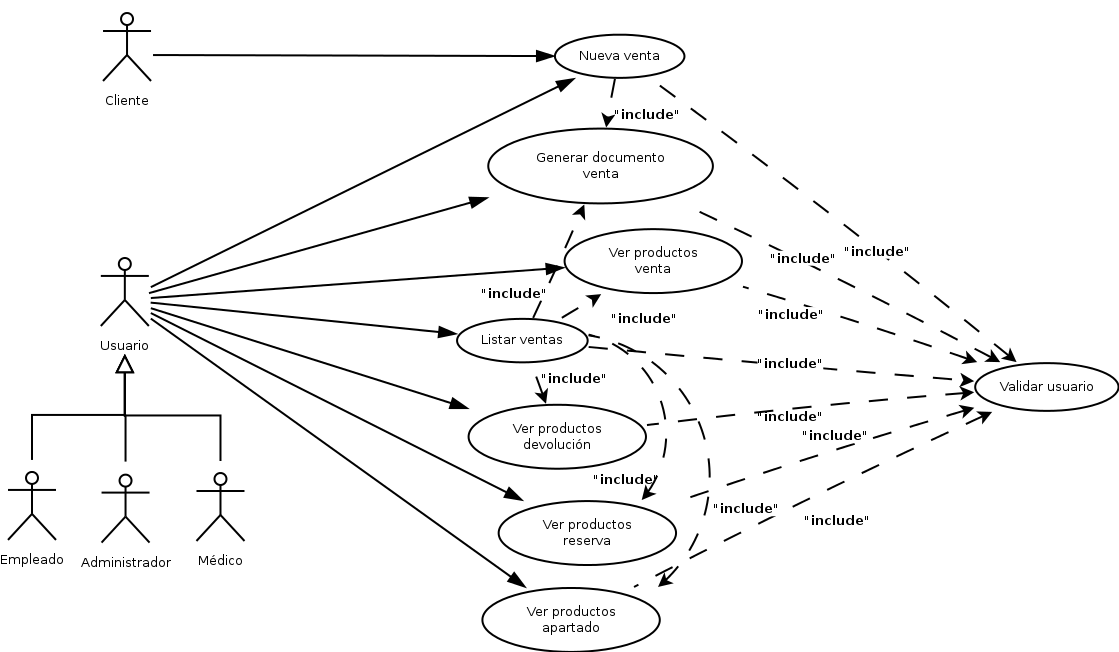
\includegraphics[scale=0.4]{gestionventas.png}
  \caption{Diagrama caso de uso. Gestión ventas}
  \label{cu7}
\end{figure}
\smallskip
\hrule height 1pt
\smallskip
\textbf{Caso de uso: Nueva venta}
\begin{itemize}\renewcommand{\labelitemi}{$\cdot$}
  \item \textbf{Descripción:} El usuario introduce los datos para registrar una nueva venta en el sistema.
  \item \textbf{Actores:} Usuario(Principal), Cliente (Secundario)
  \item \textbf{Precondiciones:} Se debe comprobar que el usuario este autenticado en el sistema con el caso de uso Validar usuario.
  \item \textbf{Postcondiciones:} El usuario almacena la venta en el sistema.
\end{itemize}
\underline{\textbf{Identificación de escenarios:}}
\begin{itemize}\renewcommand{\labelitemi}{$\circ$}
 \item \textbf{Escenario principal:}
         \begin{enumerate}
          \item El caso de uso se inicia cuando el usuario decide crear una nueva venta.
 	 \item El sistema muestra por pantalla todos los clientes para que se puedan seleccionar.
	\item El usuario selecciona el cliente al que quiere realizar la venta.
          \item El sistema muestra por pantalla todos los productos para que se puedan seleccionar.
          \item El usuario introduce los productos y cantidades que desea introducir en la venta.
          \item El sistema comprueba que los datos introducidos son correctos.
	  \item El usuario introduce la forma de pago tarjeta.
  	  \item El sistema muestra un mensaje de confirmación.
          \item El usuario pulsa SI en el mensaje de confirmación.
	  \item El sistema actualiza los stocks de los productos.
 	  \item El sistema almacena el cambio del sistema (auditoria).
          \item La venta queda almacenada en el sistema y se muestra un mensaje de éxito.
         \end{enumerate}
  \item \textbf{Escenario alternativos:}\\\\
	  6a. El usuario introduce de manera incorrecta los datos.
		\begin{enumerate}
		 \item El sistema muestra el error y pide que se introduzcan nuevos datos.
		\end{enumerate}
	7a. El usuario elige el pago con efectivo.
		\begin{enumerate}
		\item El usuario introduce el dinero entregado por el cliente.
		
		 \item El sistema mostrará en el mensaje de confirmación el cambio a devolver al cliente y la venta se almacenará con forma de pago efectivo.
		\end{enumerate}
	 9a. El usuario decide no realizar la venta.
	      \begin{enumerate}
	       \item El sistema cancela el registro de una nueva venta en el sistema.
	      \end{enumerate}
         12a. El usuario elige mostrar documento de venta.
	      \begin{enumerate}
	       \item La venta queda almacenada en el sistema y se muestra por pantalla el documento de venta.
	      \end{enumerate}
          *a. El usuario cancela el proceso de nueva venta.
\end{itemize}
\smallskip
\hrule height 1pt
\smallskip
\textbf{Caso de uso: Listar ventas}
\begin{itemize}\renewcommand{\labelitemi}{$\cdot$}
 \item \textbf{Descripción:} El usuario consulta las ventas almacenadas en el sistema.
  \item \textbf{Actores:} Usuario
  \item \textbf{Precondiciones:} Se debe comprobar que el usuario este autenticado en el sistema con el caso de uso Validar usuario.
  \item \textbf{Postcondiciones:} El sistema muestra por pantalla todos las ventas almacenadas.
\end{itemize}
\underline{\textbf{Identificación de escenarios:}}
\begin{itemize}\renewcommand{\labelitemi}{$\circ$}
 \item \textbf{Escenario principal:}
         \begin{enumerate}
          \item El caso de uso se inicia cuando el usuario decide consultar las ventas.
          \item El sistema muestra la lista de todas las ventas del sistema.
          \item El usuario no selecciona un patrón de búsqueda.
          \item El sistema muestra todas las ventas.
         \end{enumerate}
  \item \textbf{Escenario alternativos:}\\
  			3a. El usuario introduce un patrón de búsqueda.
  			\begin{enumerate}
  			\item El sistema muestra los datos acordes a ese patrón de búsqueda.
  			\item El usuario puede seleccionar el patrón de búsqueda cuantas veces desee.
  			\end{enumerate}
          *a. El usuario cancela en cualquier momento la consulta de listar ventas.
\end{itemize}
\smallskip
\hrule height 1pt
\smallskip
\textbf{Caso de uso: Generar documento venta}
\begin{itemize}\renewcommand{\labelitemi}{$\cdot$}
 \item \textbf{Descripción:} El usuario decide generar un documento de una venta.
  \item \textbf{Actores:} Usuario
  \item \textbf{Precondiciones:} La venta ya existe en el sistema. Se debe comprobar que el usuario este autenticado en el sistema con el caso de uso Validar usuario.
  \item \textbf{Postcondiciones:} El sistema muestra por pantalla el documento de venta generado.
\end{itemize}
\underline{\textbf{Identificación de escenarios:}}
\begin{itemize}\renewcommand{\labelitemi}{$\circ$}
 \item \textbf{Escenario principal:}
         \begin{enumerate}
          \item El caso de uso se inicia cuando el usuario decide generar un documento a una venta.
	  \item El sistema muestra por pantalla el documento de la venta.
         \end{enumerate}
\end{itemize}
\smallskip
\hrule height 1pt
\smallskip
\textbf{Caso de uso: Ver productos venta}
\begin{itemize}\renewcommand{\labelitemi}{$\cdot$}
 \item \textbf{Descripción:} El usuario decide ver productos asociados a una venta.
  \item \textbf{Actores:} suario
  \item \textbf{Precondiciones:} La venta ya existe en el sistema. Se debe comprobar que el usuario este autenticado en el sistema con el caso de uso Validar usuario.
  \item \textbf{Postcondiciones:} El sistema muestra por pantalla los productos asociados a la venta.
\end{itemize}
\underline{\textbf{Identificación de escenarios:}}
\begin{itemize}\renewcommand{\labelitemi}{$\circ$}
 \item \textbf{Escenario principal:}
         \begin{enumerate}
          \item El caso de uso se inicia cuando el usuario decide ver los productos asociados a una venta.
	  \item El sistema muestra por pantalla los productos asociados a la venta.
         \end{enumerate}
\end{itemize}

\subsection{Requisito funcional: Gestión devoluciones}

\begin{itemize}
 \item El usuario podrá crear una nueva devolución en el sistema.
 \item El usuario podrá consultar e imprimir el listado de todas las devoluciones del sistema.
 \item El usuario podrá ver los productos asociados a una devolución.
 \item El usuario podrá realizar filtrados de las devoluciones del sistema.
 \item El usuario podrá generar documentos de devolución.

\end{itemize}
\begin{figure}[H]
  \centering
    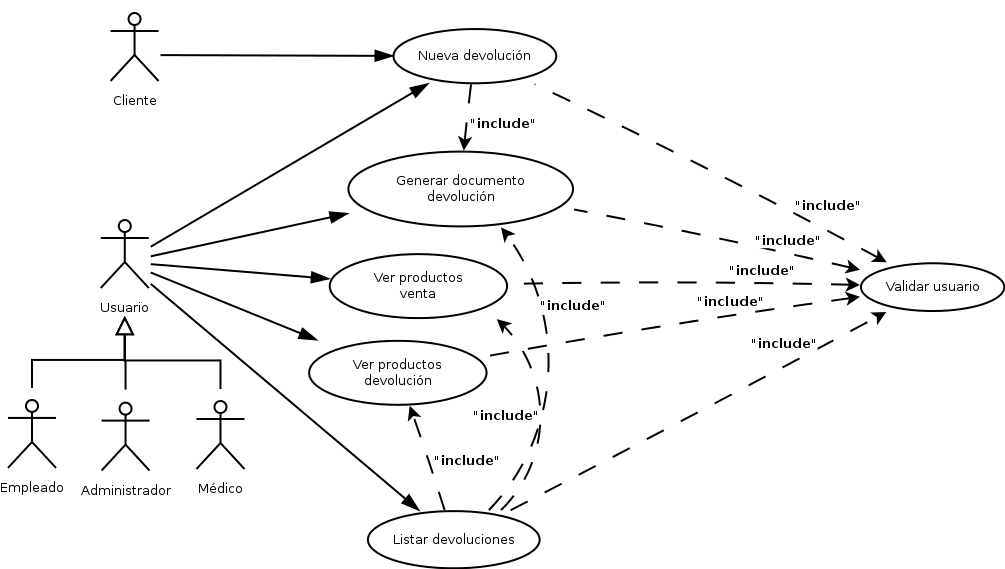
\includegraphics[scale=0.4]{gestiondevoluciones.png}
  \caption{Diagrama caso de uso. Gestión devoluciones}
  \label{cu7}
\end{figure}
\smallskip
\hrule height 1pt
\smallskip
\textbf{Caso de uso: Nueva devolución}
\begin{itemize}\renewcommand{\labelitemi}{$\cdot$}
  \item \textbf{Descripción:} El usuario introduce los datos para registrar una nueva devolución en el sistema.
  \item \textbf{Actores:} Usuario(Principal), Cliente(Secundario)
  \item \textbf{Precondiciones:} Se debe comprobar que el usuario este autenticado en el sistema con el caso de uso Validar usuario.
  \item \textbf{Postcondiciones:} El sistema almacena la devolución en el sistema.
\end{itemize}
\underline{\textbf{Identificación de escenarios:}}
\begin{itemize}\renewcommand{\labelitemi}{$\circ$}
 \item \textbf{Escenario principal:}
         \begin{enumerate}
          \item El caso de uso se inicia cuando el usuario decide crear una nueva devolución.
          \item El sistema muestra por pantalla todas las ventas del sistema para seleccionar.
	\item El usuario selecciona una venta para realizarle la devolución.
          \item El usuario selecciona los productos devueltos de esa venta.
  	  \item El sistema muestra un mensaje de confirmación.
          \item El usuario pulsa SI en el mensaje de confirmación.
 	  \item El sistema almacena el cambio del sistema (auditoria).
          \item La devolución queda almacenada en el sistema y se muestra un mensaje de éxito.
         \end{enumerate}
  \item \textbf{Escenario alternativos:}\\\\
	 4a. El usuario no selecciona ningún producto a devolver.
	      \begin{enumerate}
	       \item El sistema muestra el error y espera que se introduzcan nuevos datos.
	      \end{enumerate}
	 6a. El usuario decide no realizar la devolución.
	      \begin{enumerate}
	       \item El sistema cancela el registro de una nueva devolución en el sistema.
	      \end{enumerate}
         8a. El usuario elige mostrar documento.
	      \begin{enumerate}
	       \item La devolución queda almacenada en el sistema y se muestra el documento por pantalla.
	      \end{enumerate}
          *a. El usuario cancela el proceso de nueva devolución.
\end{itemize}
\smallskip
\hrule height 1pt
\smallskip
\textbf{Caso de uso: Listar devoluciones}
\begin{itemize}\renewcommand{\labelitemi}{$\cdot$}
 \item \textbf{Descripción:} El usuario consulta las devoluciones almacenadas en el sistema.
  \item \textbf{Actores:} Usuario
  \item \textbf{Precondiciones:} Se debe comprobar que el usuario este autenticado en el sistema con el caso de uso Validar usuario.
  \item \textbf{Postcondiciones:} El sistema muestra por pantalla todas las devoluciones almacenadas.
\end{itemize}
\underline{\textbf{Identificación de escenarios:}}
\begin{itemize}\renewcommand{\labelitemi}{$\circ$}
 \item \textbf{Escenario principal:}
         \begin{enumerate}
          \item El caso de uso se inicia cuando el usuario decide consultar las devoluciones.
          \item El sistema muestra la lista de todas las devoluciones del sistema.
          \item El usuario no selecciona un patrón de búsqueda.
          \item El sistema muestra todas las devoluciones.
         \end{enumerate}
  \item \textbf{Escenario alternativos:}\\
  			3a. El usuario introduce un patrón de búsqueda.
  			\begin{enumerate}
  			\item El sistema muestra los datos acordes a ese patrón de búsqueda.
  			\item El usuario puede seleccionar el patrón de búsqueda cuantas veces desee.
  			\end{enumerate}
          *a. El usuario cancela en cualquier momento la consulta de listar devoluciones.
\end{itemize}
\smallskip
\hrule height 1pt
\smallskip
\textbf{Caso de uso: Generar documento devolución}
\begin{itemize}\renewcommand{\labelitemi}{$\cdot$}
 \item \textbf{Descripción:} El usuario decide generar un documento de una devolución.
  \item \textbf{Actores:} Usuario
  \item \textbf{Precondiciones:} La devolución ya existe en el sistema. Se debe comprobar que el usuario este autenticado en el sistema con el caso de uso Validar usuario.
  \item \textbf{Postcondiciones:} El sistema muestra por pantalla el documento devolución generado.
\end{itemize}
\underline{\textbf{Identificación de escenarios:}}
\begin{itemize}\renewcommand{\labelitemi}{$\circ$}
 \item \textbf{Escenario principal:}
         \begin{enumerate}
          \item El caso de uso se inicia cuando el usuario decide generar un documento de devolución.
	  \item El sistema muestra por pantalla el documento de devolución.
         \end{enumerate}
\end{itemize}

\smallskip
\hrule height 1pt
\smallskip
\textbf{Caso de uso: Ver productos devolución}
\begin{itemize}\renewcommand{\labelitemi}{$\cdot$}
 \item \textbf{Descripción:} El usuario decide ver productos devueltos de una venta.
  \item \textbf{Actores:} Usuario
  \item \textbf{Precondiciones:} La venta ya existe en el sistema. Se debe comprobar que el usuario este autenticado en el sistema con el caso de uso Validar usuario.
  \item \textbf{Postcondiciones:} El sistema muestra por pantalla los productos devueltos de una venta.
\end{itemize}
\underline{\textbf{Identificación de escenarios:}}
\begin{itemize}\renewcommand{\labelitemi}{$\circ$}
 \item \textbf{Escenario principal:}
         \begin{enumerate}
          \item El caso de uso se inicia cuando el usuario decide ver los productos devueltos de una venta.
          \item El usuario indica la fecha de la devolución.
	  \item El sistema muestra por pantalla los productos devueltos de la venta en esa fecha.
         \end{enumerate}
\end{itemize}

\subsection{Requisito funcional: Gestión reservas}

\begin{itemize}
 \item El usuario podrá crear una nueva reserva en el sistema.
 \item El usuario podrá consultar e imprimir el listado de todas las reservas del sistema.
 \item El usuario podrá ver los productos asociados a una reserva.
 \item El usuario podrá realizar filtrados de las reservas del sistema.
 \item El usuario podrá generar documentos de reservas.
\item El usuario podrá avisar al cliente cuando el producto vuelva a estar disponible.
\item El usuario podrá convertir a venta una reserva.

\end{itemize}
\begin{figure}[H]
  \centering
    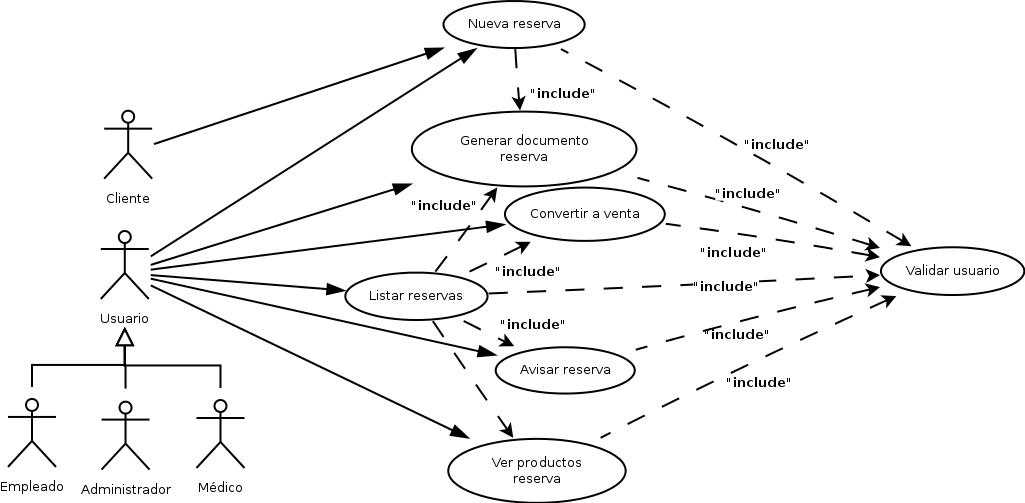
\includegraphics[scale=0.4]{gestionreservas.png}
  \caption{Diagrama caso de uso. Gestión reservas}
  \label{cu7}
\end{figure}
\smallskip
\hrule height 1pt
\smallskip
\textbf{Caso de uso: Nueva reserva}
\begin{itemize}\renewcommand{\labelitemi}{$\cdot$}
  \item \textbf{Descripción:} El usuario introduce los datos para registrar una nueva reserva en el sistema.
  \item \textbf{Actores:} Usuario(Principal), Cliente(Secundario)
  \item \textbf{Precondiciones:} Se debe comprobar que el usuario este autenticado en el sistema con el caso de uso Validar usuario.
  \item \textbf{Postcondiciones:} El usuario almacena la reserva en el sistema.
\end{itemize}
\underline{\textbf{Identificación de escenarios:}}
\begin{itemize}\renewcommand{\labelitemi}{$\circ$}
 \item \textbf{Escenario principal:}
         \begin{enumerate}
          \item El caso de uso se inicia cuando el usuario decide crear una nueva reserva.
	\item El sistema muestra por pantalla todos los clientes para que se puedan seleccionar.
	\item El usuario selecciona el cliente para realizar la reserva.
	\item El sistema muestra por pantalla todos los productos para que se puedan seleccionar.
          \item El usuario introduce los productos y cantidades para la nueva reserva.
	  \item El sistema comprueba que los datos introducidos son correctos.
	 \item El usuario introduce el adelanto del cliente.
	  \item El usuario introduce la forma de pago tarjeta.
  	  \item El sistema muestra un mensaje de confirmación.
          \item El usuario pulsa SI en el mensaje de confirmación.
 	  \item El sistema almacena el cambio del sistema (auditoria).
          \item La reserva queda almacenada en el sistema y se muestra un mensaje de éxito.
         \end{enumerate}
  \item \textbf{Escenario alternativos:}\\\\
	  6a. El usuario introduce de manera incorrecta los datos.
		\begin{enumerate}
		 \item El sistema muestra el error y pide que se introduzcan nuevos datos.
		\end{enumerate}
	7a. El usuario introduce de manera incorrecta el adelanto.
		\begin{enumerate}
		 \item El sistema muestra el error y pide que se introduzca de nuevo el adelanto.
		\end{enumerate}
	8a. El usuario elige el pago con efectivo.
		\begin{enumerate}
		\item El usuario introduce el dinero entregado por el cliente.
		 \item El sistema mostrará en el mensaje de confirmación el cambio a devolver al cliente y la reserva se almacenará con forma de pago efectivo.
		\end{enumerate}
	 10a. El usuario decide no realizar la reserva.
	      \begin{enumerate}
	       \item El sistema cancela el registro de una nueva reserva en el sistema.
	      \end{enumerate}
         12a. El usuario elige mostrar documento reserva.
	      \begin{enumerate}
	       \item La reserva queda almacenada en el sistema y se muestra el documento reserva por pantalla.
	      \end{enumerate}
          *a. El usuario cancela el proceso de nueva reserva.
\end{itemize}
\smallskip
\hrule height 1pt
\smallskip
\textbf{Caso de uso: Listar reservas}
\begin{itemize}\renewcommand{\labelitemi}{$\cdot$}
 \item \textbf{Descripción:} El usuario consulta las reservas almacenadas en el sistema.
  \item \textbf{Actores:} Usuario
  \item \textbf{Precondiciones:} Se debe comprobar que el usuario este autenticado en el sistema con el caso de uso Validar usuario.
  \item \textbf{Postcondiciones:} El sistema muestra por pantalla todas las reservas almacenadas.
\end{itemize}
\underline{\textbf{Identificación de escenarios:}}
\begin{itemize}\renewcommand{\labelitemi}{$\circ$}
 \item \textbf{Escenario principal:}
         \begin{enumerate}
          \item El caso de uso se inicia cuando el usuario decide consultar las reservas.
          \item El sistema muestra la lista de todas las reservas del sistema.
          \item El usuario no selecciona un patrón de búsqueda.
          \item El sistema muestra todas las reservas.
         \end{enumerate}
  \item \textbf{Escenario alternativos:}\\
  			3a. El usuario introduce un patrón de búsqueda.
  			\begin{enumerate}
  			\item El sistema muestra los datos acordes a ese patrón de búsqueda.
  			\item El usuario puede seleccionar el patrón de búsqueda cuantas veces desee.
  			\end{enumerate}
         *a. El usuario cancela en cualquier momento la consulta de listar reservas.
\end{itemize}
\smallskip
\hrule height 1pt
\smallskip
\textbf{Caso de uso: Generar documento reserva}
\begin{itemize}\renewcommand{\labelitemi}{$\cdot$}
 \item \textbf{Descripción:} El usuario decide generar un documento de una reserva.
  \item \textbf{Actores:} Usuario
  \item \textbf{Precondiciones:} La reserva ya existe en el sistema. Se debe comprobar que el usuario este autenticado en el sistema con el caso de uso Validar usuario.
  \item \textbf{Postcondiciones:} El sistema muestra por pantalla el documento reserva generado.
\end{itemize}
\underline{\textbf{Identificación de escenarios:}}
\begin{itemize}\renewcommand{\labelitemi}{$\circ$}
 \item \textbf{Escenario principal:}
         \begin{enumerate}
          \item El caso de uso se inicia cuando el usuario decide generar un documento de reserva.
	  \item El sistema muestra por pantalla el documento de reserva.
         \end{enumerate}
\end{itemize}

\smallskip
\hrule height 1pt
\smallskip
\textbf{Caso de uso: Convertir a venta}
\begin{itemize}\renewcommand{\labelitemi}{$\cdot$}
 \item \textbf{Descripción:} El usuario decide convertir a venta una reserva.
  \item \textbf{Actores:} Usuario
  \item \textbf{Precondiciones:} La reserva ya existe en el sistema. Se debe comprobar que el usuario este autenticado en el sistema con el caso de uso Validar usuario.
  \item \textbf{Postcondiciones:} El sistema almacena una nueva venta asociada con la reserva.
\end{itemize}
\underline{\textbf{Identificación de escenarios:}}
\begin{itemize}\renewcommand{\labelitemi}{$\circ$}
 \item \textbf{Escenario principal:}
         \begin{enumerate}
          \item El caso de uso se inicia cuando el usuario decide convertir una reserva en venta.
	  \item El sistema muestra un mensaje de lo que queda por pagar.
	  \item El usuario introduce la forma de pago tarjeta.
	  \item El sistema muestra un mensaje de confirmación.
	  \item El usuario pulsa en SI en el mensaje.
	  \item EL sistema actualiza la cantidad de los productos reservados.
	  \item El sistema almacena el cambio del sistema (auditoria).
	  \item El sistema almacena la venta asociada a esa reserva y muestra un mensaje por pantalla
         \end{enumerate}
\item \textbf{Escenario alternativos:}\\\\
	3a. El usuario elige el pago con efectivo.
		\begin{enumerate}
		\item El usuario introduce el dinero entregado por el cliente.
		 \item El sistema mostrará en el mensaje de confirmación el cambio a devolver al cliente y la venta se almacenará con forma de pago efectivo.
		\end{enumerate}
	 5a. El usuario decide no realizar la operación.
	      \begin{enumerate}
	       \item El sistema cancela el registro de una nueva venta de la reserva.
	      \end{enumerate}
         6a. El usuario elige mostrar documento venta.
	      \begin{enumerate}
	       \item La venta queda almacenada en el sistema y se muestra el documento venta por pantalla.
	      \end{enumerate}
          *a. El usuario cancela el proceso de nueva venta asociada a la reserva.
\end{itemize}

\smallskip
\hrule height 1pt
\smallskip
\smallskip
\textbf{Caso de uso: Avisar reserva}
\begin{itemize}\renewcommand{\labelitemi}{$\cdot$}
 \item \textbf{Descripción:} El usuario decide avisar al cliente de una reserva.
  \item \textbf{Actores:} Usuario
  \item \textbf{Precondiciones:} La reserva ya existe en el sistema. Se debe comprobar que el usuario este autenticado en el sistema con el caso de uso Validar usuario.
  \item \textbf{Postcondiciones:} El sistema almacena el aviso al cliente.
\end{itemize}
\underline{\textbf{Identificación de escenarios:}}
\begin{itemize}\renewcommand{\labelitemi}{$\circ$}
 \item \textbf{Escenario principal:}
         \begin{enumerate}
          \item El caso de uso se inicia cuando el usuario decide avisar al cliente de una reserva.
	  \item El sistema cambia las cantidades de los productos reservados por apartados.
	  \item El sistema almacena el aviso al cliente.
         \end{enumerate}
\end{itemize}

\smallskip
\hrule height 1pt
\smallskip
\textbf{Caso de uso: Ver productos reserva}
\begin{itemize}\renewcommand{\labelitemi}{$\cdot$}
 \item \textbf{Descripción:} El usuario decide ver productos reservados de una venta.
  \item \textbf{Actores:} Usuario
  \item \textbf{Precondiciones:} La reserva ya existe en el sistema. Se debe comprobar que el usuario este autenticado en el sistema con el caso de uso Validar usuario.
  \item \textbf{Postcondiciones:} El sistema muestra por pantalla los productos reservados.
\end{itemize}
\underline{\textbf{Identificación de escenarios:}}
\begin{itemize}\renewcommand{\labelitemi}{$\circ$}
 \item \textbf{Escenario principal:}
         \begin{enumerate}
          \item El caso de uso se inicia cuando el usuario decide ver los productos reservados.
	  \item El sistema muestra por pantalla los productos reservados.
         \end{enumerate}
\end{itemize}

\subsection{Requisito funcional: Gestión apartados}

\begin{itemize}
 \item El usuario podrá crear una nuevo apartado en el sistema.
 \item El usuario podrá consultar e imprimir el listado de todos los apartados del sistema.
 \item El usuario podrá ver los productos asociados a un apartado.
 \item El usuario podrá realizar filtrados de los apartados del sistema.
 \item El usuario podrá generar documentos de apartados.
\item El usuario podrá convertir a venta un apartado.

\end{itemize}
\begin{figure}[H]
  \centering
    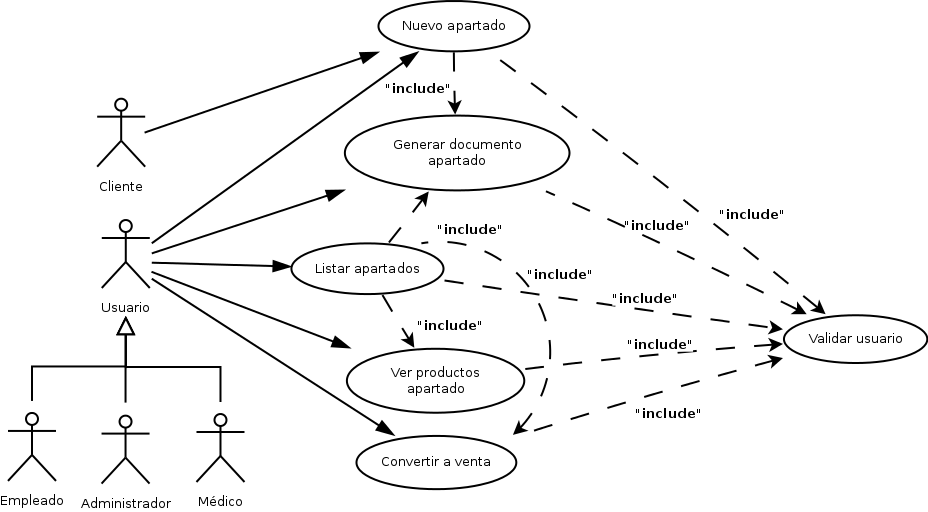
\includegraphics[scale=0.4]{gestionapartados.png}
  \caption{Diagrama caso de uso. Gestión apartados}
  \label{cu7}
\end{figure}
\smallskip
\hrule height 1pt
\smallskip
\textbf{Caso de uso: Nuevo apartado}
\begin{itemize}\renewcommand{\labelitemi}{$\cdot$}
  \item \textbf{Descripción:} El usuario introduce los datos para registrar un nuevo apartado en el sistema.
  \item \textbf{Actores:} Usuario(Principal), Cliente(Secundario)
  \item \textbf{Precondiciones:} Se debe comprobar que el usuario este autenticado en el sistema con el caso de uso Validar usuario.
  \item \textbf{Postcondiciones:} El usuario almacena el apartado en el sistema.
\end{itemize}
\underline{\textbf{Identificación de escenarios:}}
\begin{itemize}\renewcommand{\labelitemi}{$\circ$}
 \item \textbf{Escenario principal:}
         \begin{enumerate}
          \item El caso de uso se inicia cuando el usuario decide crear un nuevo apartado.
	\item El sistema muestra por pantalla todos los clientes para que se puedan seleccionar.
	\item El usuario selecciona al cliente al que quiere realizar el apartado.
	\item El sistema muestra por pantalla todos los productos para que se puedan seleccionar.
          \item El usuario introduce los productos y cantidades para el nuevo apartado.
	  \item El sistema comprueba que los datos introducidos son correctos.
	\item El usuario introduce el adelanto del cliente.
	  \item El usuario introduce la forma de pago tarjeta.
  	  \item El sistema muestra un mensaje de confirmación.
          \item El usuario pulsa SI en el mensaje de confirmación.
 	  \item El sistema almacena el cambio del sistema (auditoria).
          \item El apartado queda almacenado en el sistema y se muestra un mensaje de éxito.
         \end{enumerate}
  \item \textbf{Escenario alternativos:}\\\\
	  6a. El usuario introduce de manera incorrecta los datos.
		\begin{enumerate}
		 \item El sistema muestra el error y pide que se introduzcan nuevos datos.
		\end{enumerate}
	7a. El usuario introduce de manera incorrecta el adelanto.
		\begin{enumerate}
		 \item El sistema muestra el error y pide que se introduzca de nuevo el adelanto.
		\end{enumerate}
	8a. El usuario elige el pago con efectivo.
		\begin{enumerate}
		 \item El usuario introduce el dinero entregado por el cliente.
		 \item El sistema mostrará en el mensaje de confirmación el cambio a devolver al cliente y la venta se almacenará con forma de pago efectivo.
		\end{enumerate}
	 10a. El usuario decide no realizar el apartado.
	      \begin{enumerate}
	       \item El sistema cancela el registro de un nuevo apartado en el sistema.
	      \end{enumerate}
         12a. El usuario elige mostrar documento apartado.
	      \begin{enumerate}
	       \item El apartado queda almacenado en el sistema y se muestra el documento de apartado por pantalla.
	      \end{enumerate}
          *a. El usuario cancela el proceso de nuevo apartado.
\end{itemize}
\smallskip
\hrule height 1pt
\smallskip
\textbf{Caso de uso: Listar apartados}
\begin{itemize}\renewcommand{\labelitemi}{$\cdot$}
 \item \textbf{Descripción:} El usuario consulta los apartados almacenados en el sistema.
  \item \textbf{Actores:} Usuario
  \item \textbf{Precondiciones:} Se debe comprobar que el usuario este autenticado en el sistema con el caso de uso Validar usuario.
  \item \textbf{Postcondiciones:} El sistema muestra por pantalla todos los apartados almacenados.
\end{itemize}
\underline{\textbf{Identificación de escenarios:}}
\begin{itemize}\renewcommand{\labelitemi}{$\circ$}
 \item \textbf{Escenario principal:}
         \begin{enumerate}
          \item El caso de uso se inicia cuando el usuario decide consultar los apartados.
          \item El sistema muestra la lista de todos los apartados del sistema.
          \item El usuario no selecciona un patrón de búsqueda.
          \item El sistema muestra todos los apartados.
         \end{enumerate}
  \item \textbf{Escenario alternativos:}\\
  			3a. El usuario introduce un patrón de búsqueda.
  			\begin{enumerate}
  			\item El sistema muestra los datos acordes a ese patrón de búsqueda.
  			\item El usuario puede seleccionar el patrón de búsqueda cuantas veces desee.
  			\end{enumerate}
         *a. El usuario cancela en cualquier momento la consulta de listar apartados.
\end{itemize}
\smallskip
\hrule height 1pt
\smallskip
\textbf{Caso de uso: Generar documento apartado}
\begin{itemize}\renewcommand{\labelitemi}{$\cdot$}
 \item \textbf{Descripción:} El usuario decide generar un documento de un apartado.
  \item \textbf{Actores:} Usuario
  \item \textbf{Precondicones:} El apartado ya existe en el sistema. Se debe comprobar que el usuario este autenticado en el sistema con el caso de uso Validar usuario.
  \item \textbf{Postcondiciones:} El sistema muestra por pantalla el documento apartado generado.
\end{itemize}
\underline{\textbf{Identificación de escenarios:}}
\begin{itemize}\renewcommand{\labelitemi}{$\circ$}
 \item \textbf{Escenario principal:}
         \begin{enumerate}
          \item El caso de uso se inicia cuando el usuario decide generar un documento de apartado.
	  \item El sistema muestra por pantalla el documento de apartado.
         \end{enumerate}
\end{itemize}

\smallskip
\hrule height 1pt
\smallskip
\textbf{Caso de uso: Convertir a venta}
\begin{itemize}\renewcommand{\labelitemi}{$\cdot$}
 \item \textbf{Descripción:} El usuario decide convertir a venta un apartado.
  \item \textbf{Actores:} Usuario
  \item \textbf{Precondiciones:} El apartado ya existe en el sistema. Se debe comprobar que el usuario este autenticado en el sistema con el caso de uso Validar usuario.
  \item \textbf{Postcondiciones:} El sistema almacena una nueva venta asociada con el apartado.
\end{itemize}
\underline{\textbf{Identificación de escenarios:}}
\begin{itemize}\renewcommand{\labelitemi}{$\circ$}
 \item \textbf{Escenario principal:}
         \begin{enumerate}
          \item El caso de uso se inicia cuando el usuario decide convertir un apartado en venta.
	  \item El sistema muestra un mensaje de lo que queda por pagar.
	  \item El usuario introduce la forma de pago tarjeta.
	  \item El sistema muestra un mensaje de confirmación.
	  \item El usuario pulsa en SI en el mensaje.
	  \item EL sistema actualiza la cantidad de los productos apartados.
	  \item El sistema almacena el cambio del sistema (auditoria).
	  \item El sistema almacena la venta asociada a ese apartado y muestra un mensaje por pantalla
         \end{enumerate}
\item \textbf{Escenario alternativos:}\\\\
	3a. El usuario elige el pago con efectivo.
		\begin{enumerate}
		\item El usuario introduce el dinero entregado por el cliente.
		 \item El sistema mostrará en el mensaje de confirmación el cambio a devolver al cliente y la venta se almacenará con forma de pago efectivo.
		\end{enumerate}
	 5a. El usuario decide no realizar la operación.
	      \begin{enumerate}
	       \item El sistema cancela el registro de una nueva venta del apartado.
	      \end{enumerate}
         6a. El usuario elige mostrar documento venta.
	      \begin{enumerate}
	       \item La venta queda almacenada en el sistema y se muestra el documento venta por pantalla.
	      \end{enumerate}
          *a. El usuario cancela el proceso de nueva venta asociada al apartado.
\end{itemize}

\smallskip
\hrule height 1pt
\smallskip
\textbf{Caso de uso: Ver productos apartado}
\begin{itemize}\renewcommand{\labelitemi}{$\cdot$}
 \item \textbf{Descripción:} El usuario decide ver los productos de un apartado.
  \item \textbf{Actores:} Usuario
  \item \textbf{Precondiciones:} El apartado ya existe en el sistema. Se debe comprobar que el usuario este autenticado en el sistema con el caso de uso Validar usuario.
  \item \textbf{Postcondiciones:} El sistema muestra por pantalla los productos apartados.
\end{itemize}
\underline{\textbf{Identificación de escenarios:}}
\begin{itemize}\renewcommand{\labelitemi}{$\circ$}
 \item \textbf{Escenario principal:}
         \begin{enumerate}
          \item El caso de uso se inicia cuando el usuario decide ver los productos apartados.
	  \item El sistema muestra por pantalla los productos apartados.
         \end{enumerate}
\end{itemize}

\subsection{Requisito funcional: Gestión citas e informes}

\begin{itemize}
 \item El usuario podrá crear una nueva cita en el sistema.
 \item El usuario podrá consultar un informe en el sistema.
 \item El usuario podrá eliminar una cita del sistema.
 \item El usuario podrá consultar e imprimir el listado de todas las citas del sistema.
 \item El usuario podrá realizar filtrados de las citas del sistema.
 \item El usuario podrá consultar e imprimir el listado de todos los informes del sistema.
 \item El usuario podrá realizar filtrados de los informes del sistema. 
 \item El médico podrá crear un nuevo informe sin cita en el sistema.
 \item El médico podrá crear un nuevo informe con cita en el sistema.

\end{itemize}
\begin{figure}[H]
  \centering
    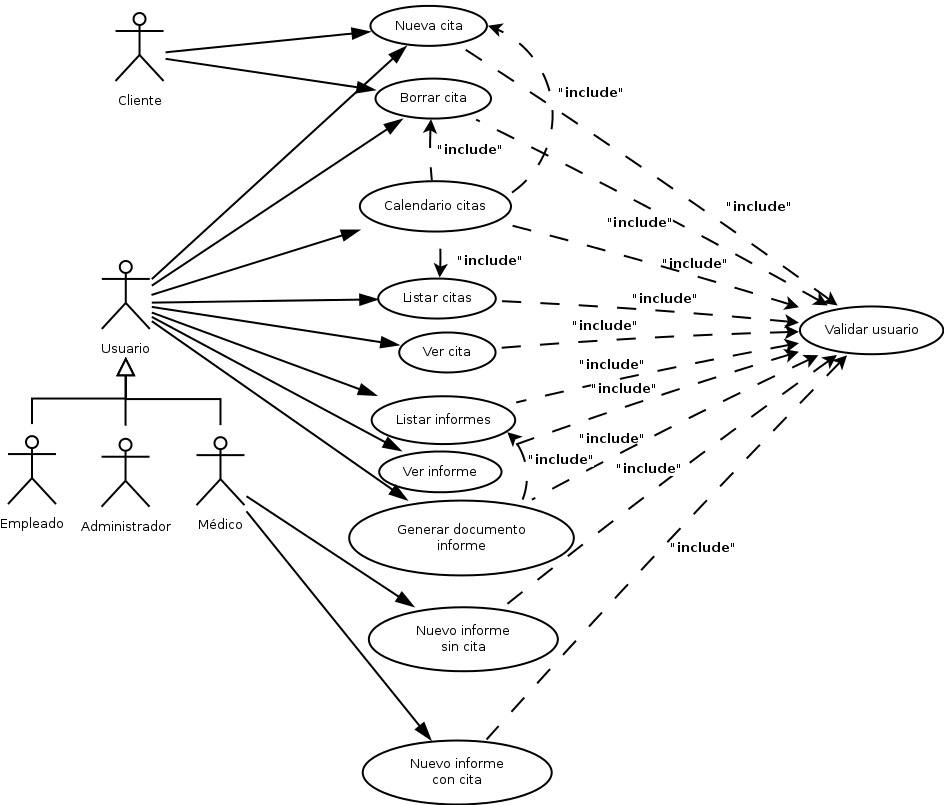
\includegraphics[scale=0.5]{gestioncitaseinformes.png}
  \caption{Diagrama caso de uso. Gestión citas e informes}
  \label{cu8}
\end{figure}
\smallskip
\hrule height 1pt
\smallskip
\textbf{Caso de uso: Nueva cita}
\begin{itemize}\renewcommand{\labelitemi}{$\cdot$}
  \item \textbf{Descripción:} El usuario introduce los datos para registrar una nueva cita en el sistema.
  \item \textbf{Actores:} Usuario(Principal) Cliente(Secundario)
  \item \textbf{Precondiciones:} Se debe comprobar que el usuario este autenticado en el sistema con el caso de uso Validar usuario.
  \item \textbf{Postcondiciones:} El usuario almacena la cita en el sistema.
\end{itemize}
\underline{\textbf{Identificación de escenarios:}}
\begin{itemize}\renewcommand{\labelitemi}{$\circ$}
 \item \textbf{Escenario principal:}
         \begin{enumerate}
          \item El caso de uso se inicia cuando el usuario decide crear una nueva cita.
          \item El usuario selecciona el dia que quiere crear la cita.
	  \item El sistema muestra por pantalla los clientes y los médicos para que el usuario seleccione.
	  \item El usuario introduce el cliente y el médico de la cita.
          \item El sistema comprueba que los datos introducidos son correctos.
 	  \item El sistema almacena el cambio del sistema (auditoria).
          \item La cita queda almacenada en el sistema y se muestra por pantalla.
         \end{enumerate}
  \item \textbf{Escenario alternativos:}\\\\
	5a. La fecha introducida esta ocupada por el médico o el cliente.
		\begin{enumerate}
		 \item El sistema muestra el error y pide que se introduzcan nuevos datos.
		\end{enumerate}
          *a. El usuario cancela en cualquier momento el proceso de nueva cita.
\end{itemize}
\smallskip
\hrule height 1pt
\smallskip
\textbf{Caso de uso: Borrar cita}
\begin{itemize}\renewcommand{\labelitemi}{$\cdot$}
 \item \textbf{Descripción:} El usuario decide borrar una cita del sistema.
  \item \textbf{Actores:} Usuario(Principal), Cliente(Secundario)
  \item \textbf{Precondiciones:} La cita existe en el sistema. Se debe comprobar que el usuario este autenticado en el sistema con el caso de uso Validar usuario.
  \item \textbf{Postcondiciones:} El sistema elimina la cita del sistema.
\end{itemize}
\underline{\textbf{Identificación de escenarios:}}
\begin{itemize}\renewcommand{\labelitemi}{$\circ$}
 \item \textbf{Escenario principal:}
         \begin{enumerate}
          \item El caso de uso se inicia cuando el usuario decide borrar una cita.
          \item El usuario selecciona la cita que quiere eliminar.
          \item El sistema muestra un mensaje de confirmación.
          \item El administrador pulsa SI en el mensaje de confirmación.
 	  \item El sistema almacena el cambio del sistema (auditoria).
          \item El sistema elimina la cita seleccionada.
         \end{enumerate}
  \item \textbf{Escenario alternativos:}\\
  			4a. El usuario cancela en el mensaje de confirmación.
  			\begin{enumerate}
  			\item El sistema cancela el proceso de eliminación de una cita.
  			\end{enumerate}
          *a. El usuario cancela en cualquier momento la eliminación de una cita.
\end{itemize}
\smallskip
\hrule height 1pt
\smallskip

\textbf{Caso de uso: Listar citas}
\begin{itemize}\renewcommand{\labelitemi}{$\cdot$}
 \item \textbf{Descripción:} El usuario decide listar todas las citas del sistema.
  \item \textbf{Actores:} Usuario
  \item \textbf{Precondiciones:} Se debe comprobar que el usuario este autenticado en el sistema con el caso de uso Validar usuario.
  \item \textbf{Postcondiciones:} El sistema muestra un listado de todas las citas del sistema.
\end{itemize}
\underline{\textbf{Identificación de escenarios:}}
\begin{itemize}\renewcommand{\labelitemi}{$\circ$}
 \item \textbf{Escenario principal:}
         \begin{enumerate}
          \item El caso de uso se inicia cuando el usuario decide listar las citas del sistema.
	  \item El sistema muestra por pantalla todas las citas del sistema.
         \end{enumerate}
\end{itemize}

\smallskip
\hrule height 1pt
\smallskip

\textbf{Caso de uso: Calendario citas}
\begin{itemize}\renewcommand{\labelitemi}{$\cdot$}
 \item \textbf{Descripción:} El usuario decide mostrar en el calendario todas las citas del sistema.
  \item \textbf{Actores:} Usuario
  \item \textbf{Precondiciones:} Se debe comprobar que el usuario este autenticado en el sistema con el caso de uso Validar usuario.
  \item \textbf{Postcondiciones:} El sistema muestra un calendario con todas las citas del sistema.
\end{itemize}
\underline{\textbf{Identificación de escenarios:}}
\begin{itemize}\renewcommand{\labelitemi}{$\circ$}
 \item \textbf{Escenario principal:}
         \begin{enumerate}
          \item El caso de uso se inicia cuando el usuario decide consultar el calendario de citas del sistema.
	  \item El sistema muestra por pantalla todas las citas del sistema en el calendario.
         \end{enumerate}
\end{itemize}

\smallskip
\hrule height 1pt
\smallskip
\textbf{Caso de uso: Listar informes}
\begin{itemize}\renewcommand{\labelitemi}{$\cdot$}
 \item \textbf{Descripción:} El usuario decide listar todos los informes del sistema.
  \item \textbf{Actores:} Usuario
  \item \textbf{Precondiciones:} Se debe comprobar que el usuario este autenticado en el sistema con el caso de uso Validar usuario.
  \item \textbf{Postcondiciones:} El sistema muestra un listado de todos los informes del sistema.
\end{itemize}
\underline{\textbf{Identificación de escenarios:}}
\begin{itemize}\renewcommand{\labelitemi}{$\circ$}
 \item \textbf{Escenario principal:}
         \begin{enumerate}
          \item El caso de uso se inicia cuando el usuario decide listar los informes.
	  \item El sistema muestra por pantalla todos los informes del sistema.
         \end{enumerate}
\end{itemize}

\smallskip
\hrule height 1pt
\smallskip
\textbf{Caso de uso: Nuevo informe con cita}
\begin{itemize}\renewcommand{\labelitemi}{$\cdot$}
 \item \textbf{Descripción:} El médico decide crear un informe de una cita.
  \item \textbf{Actores:} Médico
  \item \textbf{Precondiciones:} La cita ya existe en el sistema. Se debe comprobar que el médico este autenticado en el sistema con el caso de uso Validar usuario.
  \item \textbf{Postcondiciones:} El sistema guarda en el sistema y muestra el informe de la cita.
\end{itemize}
\underline{\textbf{Identificación de escenarios:}}
\begin{itemize}\renewcommand{\labelitemi}{$\circ$}
 \item \textbf{Escenario principal:}
         \begin{enumerate}
          \item El caso de uso se inicia cuando el médico decide crear un informe de una cita.
          \item El sistema muestra las citas que le pertenecen.
          \item El médico selecciona la cita a la que generar el informe.
          \item El médico introduce los datos del informe.
	  \item El sistema muestra un mensaje de confirmación.
          \item El médico pulsa SI en el mensaje de confirmación.
 	  \item El sistema almacena el cambio del sistema (auditoria).
	  \item El sistema almacena y muestra por pantalla el nuevo informe.
         \end{enumerate}
\item \textbf{Escenario alternativos:}\\
  			6a. El usuario indica NO en el mensaje de confirmación.
  			\begin{enumerate}
  			\item El sistema cancela el proceso de generar un nuevo informe con cita.
  			\end{enumerate}
          *a. El médico cancela en cualquier momento la generación de un nuevo informe con cita.
\end{itemize}

\smallskip
\hrule height 1pt
\smallskip
\textbf{Caso de uso: Nuevo informe sin cita}
\begin{itemize}\renewcommand{\labelitemi}{$\cdot$}
 \item \textbf{Descripción:} El médico decide crear un informe de un cliente.
  \item \textbf{Actores:} Médico
  \item \textbf{Precondiciones:} Se debe comprobar que el médico este autenticado en el sistema con el caso de uso Validar usuario.
  \item \textbf{Postcondiciones:} El sistema guarda en el sistema una nueva cita y muestra el informe generado asociado.
\end{itemize}
\underline{\textbf{Identificación de escenarios:}}
\begin{itemize}\renewcommand{\labelitemi}{$\circ$}
 \item \textbf{Escenario principal:}
         \begin{enumerate}
          \item El caso de uso se inicia cuando el médico decide crear un informe de un cliente.
	  \item El sistema muestra una lista con todos los clientes del sistema.
          \item El médico selecciona el cliente al cual generar el informe.
          \item El médico introduce los datos del informe.
	  \item El sistema muestra un mensaje de confirmación.
          \item El médico pulsa SI en el mensaje de confirmación.
 	  \item El sistema almacena el cambio del sistema (auditoria).
	  \item El sistema crea una nueva cita. Almacena y muestra por pantalla el nuevo informe.
         \end{enumerate}
\item \textbf{Escenario alternativos:}\\
  			6a. El usuario indica NO en el mensaje de confirmación.
  			\begin{enumerate}
  			\item El sistema cancela el proceso de generar un nuevo informe sin cita.
  			\end{enumerate}
          *a. El médico cancela en cualquier momento la generación de un informe a un cliente.
\end{itemize}


\smallskip
\hrule height 1pt
\smallskip
\textbf{Caso de uso: Ver cita}
\begin{itemize}\renewcommand{\labelitemi}{$\cdot$}
 \item \textbf{Descripción:} El usuario decide consultar una cita del sistema.
  \item \textbf{Actores:} Usuario
  \item \textbf{Precondiciones:} Se debe comprobar que el usuario este autenticado en el sistema con el caso de uso Validar usuario.
  \item \textbf{Postcondiciones:} El sistema muestra por pantalla la información de la cita del cliente.
\end{itemize}
\underline{\textbf{Identificación de escenarios:}}
\begin{itemize}\renewcommand{\labelitemi}{$\circ$}
 \item \textbf{Escenario principal:}
         \begin{enumerate}
          \item El caso de uso se inicia cuando el usuario decide consultar una cita.
	  \item El sistema muestra la cita del cliente por pantalla.
         \end{enumerate}
\end{itemize}

\smallskip
\hrule height 1pt
\smallskip
\textbf{Caso de uso: Ver informe}
\begin{itemize}\renewcommand{\labelitemi}{$\cdot$}
 \item \textbf{Descripción:} El usuario decide consultar un informe de un cliente del sistema.
  \item \textbf{Actores:} Usuario
  \item \textbf{Precondiciones:} Se debe comprobar que el usuario este autenticado en el sistema con el caso de uso Validar usuario.
  \item \textbf{Postcondiciones:} El sistema muestra por pantalla el informe del cliente.
\end{itemize}
\underline{\textbf{Identificación de escenarios:}}
\begin{itemize}\renewcommand{\labelitemi}{$\circ$}
 \item \textbf{Escenario principal:}
         \begin{enumerate}
          \item El caso de uso se inicia cuando el usuario decide consultar un informe.
	  \item El sistema muestra por pantalla el informe del cliente.
         \end{enumerate}
\end{itemize}

\smallskip
\hrule height 1pt
\smallskip
\textbf{Caso de uso: Generar documento informe}
\begin{itemize}\renewcommand{\labelitemi}{$\cdot$}
 \item \textbf{Descripción:} El usuario decide generar un documento de un informe.
  \item \textbf{Actores:} Usuario
  \item \textbf{Precondicones:} El informe ya existe en el sistema. Se debe comprobar que el usuario este autenticado en el sistema con el caso de uso Validar usuario.
  \item \textbf{Postcondiciones:} El sistema muestra por pantalla el documento informe generado.
\end{itemize}
\underline{\textbf{Identificación de escenarios:}}
\begin{itemize}\renewcommand{\labelitemi}{$\circ$}
 \item \textbf{Escenario principal:}
         \begin{enumerate}
          \item El caso de uso se inicia cuando el usuario decide generar un documento de un cierto informe.
	  \item El sistema muestra por pantalla el documento del informe.
         \end{enumerate}
\end{itemize}

\subsection{Requisito funcional: Gestión festivos}

\begin{itemize}
 \item El administrador podrá crear un nuevo festivo en el sistema.
 \item El administrador podrá eliminar un festivo del sistema.
 \item El administrador podrá consultar e imprimir el listado de todas los festivos del sistema.
 \item El administrador podrá realizar filtrados de los festivos del sistema.

\end{itemize}
\begin{figure}[H]
  \centering
    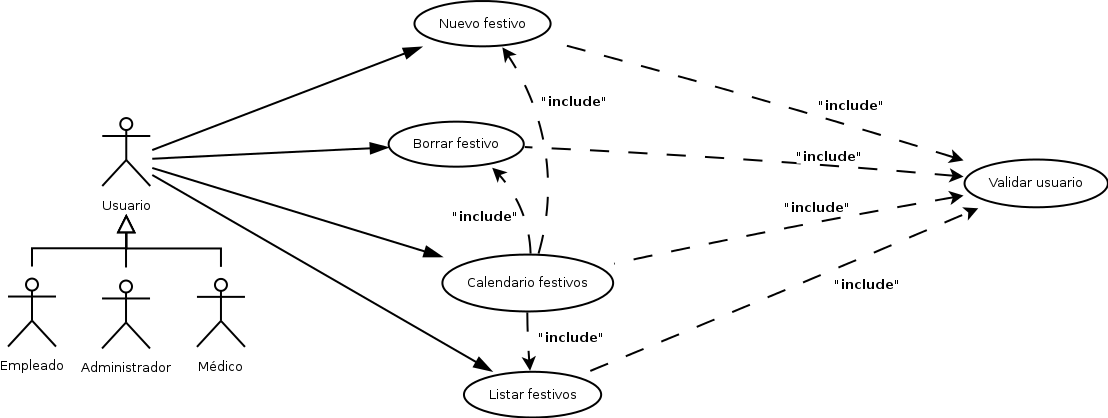
\includegraphics[scale=0.4]{gestionfestivos.png}
  \caption{Diagrama caso de uso. Gestión festivos}
  \label{cu8}
\end{figure}
\smallskip
\hrule height 1pt
\smallskip
\textbf{Caso de uso: Nuevo festivo}
\begin{itemize}\renewcommand{\labelitemi}{$\cdot$}
  \item \textbf{Descripción:} El administrador introduce los datos para registrar un nuevo festivo en el sistema.
  \item \textbf{Actores:} Administrador
  \item \textbf{Precondiciones:} Se debe comprobar que el administrador este autenticado en el sistema con el caso de uso Validar usuario.
  \item \textbf{Postcondiciones:} El usuario almacena el festivo en el sistema.
\end{itemize}
\underline{\textbf{Identificación de escenarios:}}
\begin{itemize}\renewcommand{\labelitemi}{$\circ$}
 \item \textbf{Escenario principal:}
         \begin{enumerate}
          \item El caso de uso se inicia cuando el administrador decide crear un nuevo festivo.
	  \item El sistema muestra el calendario.
          \item El usuario selecciona el día que quiere crear el festivo.
          \item El sistema comprueba que los datos introducidos son correctos.
	  \item El sistema muestra un mensaje de confirmación.
          \item El médico pulsa SI en el mensaje de confirmación.
 	  \item El sistema almacena el cambio del sistema (auditoria).
          \item El festivo queda almacenado en el sistema y se muestra por pantalla.
         \end{enumerate}
  \item \textbf{Escenario alternativos:}\\\\
	4a. El empleado elige una fecha en la cual ya existen citas.
  			\begin{enumerate}
  			\item El sistema cancela el registro de nuevo festivo y muestra el error.
  			\end{enumerate}
	6a. El usuario indica NO en el mensaje de confirmación.
  			\begin{enumerate}
  			\item El sistema cancela el proceso de generar un nuevo informe sin cita.
  			\end{enumerate}
          *a. El usuario cancela en cualquier momento el proceso de un nuevo festivo.
\end{itemize}
\smallskip
\hrule height 1pt
\smallskip
\textbf{Caso de uso: Borrar festivo}
\begin{itemize}\renewcommand{\labelitemi}{$\cdot$}
 \item \textbf{Descripción:} El administrador decide borrar un festivo del sistema.
  \item \textbf{Actores:} Administrador
  \item \textbf{Precondiciones:} El festivo ya existe en el sistema. Se debe comprobar que el administrador este autenticado en el sistema con el caso de uso Validar usuario.
  \item \textbf{Postcondiciones:} El sistema elimina el festivo del sistema.
\end{itemize}
\underline{\textbf{Identificación de escenarios:}}
\begin{itemize}\renewcommand{\labelitemi}{$\circ$}
 \item \textbf{Escenario principal:}
         \begin{enumerate}
          \item El caso de uso se inicia cuando el usuario decide borrar un festivo.
          \item El administrador selecciona el festivo que quiere eliminar.
          \item El sistema muestra un mensaje de confirmación.
          \item El administrador pulsa SI en el mensaje de confirmación.
 	  \item El sistema almacena el cambio del sistema (auditoria).
          \item El sistema elimina el festivo seleccionado.
         \end{enumerate}
  \item \textbf{Escenario alternativos:}\\
  			4a. El usuario cancela en el mensaje de confirmación.
  			\begin{enumerate}
  			\item El sistema cancela el proceso de eliminación de un festivo.
  			\end{enumerate}
          *a. El usuario cancela en cualquier momento la eliminación de un festivo.
\end{itemize}

\smallskip
\hrule height 1pt
\smallskip

\textbf{Caso de uso: Listar festivos}
\begin{itemize}\renewcommand{\labelitemi}{$\cdot$}
 \item \textbf{Descripción:} El administrador decide listar todos los festivos del sistema.
  \item \textbf{Actores:} Administrador
  \item \textbf{Precondiciones:} Se debe comprobar que el administrador este autenticado en el sistema con el caso de uso Validar usuario.
  \item \textbf{Postcondiciones:} El sistema muestra un listado de todos los festivos del sistema.
\end{itemize}
\underline{\textbf{Identificación de escenarios:}}
\begin{itemize}\renewcommand{\labelitemi}{$\circ$}
 \item \textbf{Escenario principal:}
         \begin{enumerate}
          \item El caso de uso se inicia cuando el usuario decide listar todos los festivos del sistema.
	  \item El sistema muestra por pantalla todos los festivos.
         \end{enumerate}
\end{itemize}

\smallskip
\hrule height 1pt
\smallskip
\textbf{Caso de uso: Calendario festivos}
\begin{itemize}\renewcommand{\labelitemi}{$\cdot$}
 \item \textbf{Descripción:} El usuario decide mostrar el calendario de festivos.
  \item \textbf{Actores:} Administrador
  \item \textbf{Precondiciones:} Se debe comprobar que el administrador este autenticado en el sistema con el caso de uso Validar usuario.
  \item \textbf{Postcondiciones:} El sistema muestra el calendario con todos los festivos almacenados en el sistema.
\end{itemize}
\underline{\textbf{Identificación de escenarios:}}
\begin{itemize}\renewcommand{\labelitemi}{$\circ$}
 \item \textbf{Escenario principal:}
         \begin{enumerate}
          \item El caso de uso se inicia cuando el usuario decide mostrar el calendario de festivos.
	  \item El sistema muestra por pantalla todos los festivos en el calendario.
         \end{enumerate}
\end{itemize}

\subsection{Requisito funcional: Gestión de entradas y salidas del sistema}

\begin{itemize}
 \item El usuario podrá entrar al sistema mediante un formulario de logueo.
 \item El usuario tendrá la posibilidad de recuperar la contraseña por si está ha sido olvidada.
 \item El usuario deberá salir del sistema mediante el botón "Salir".

\end{itemize}
\begin{figure}[H]
  \centering
    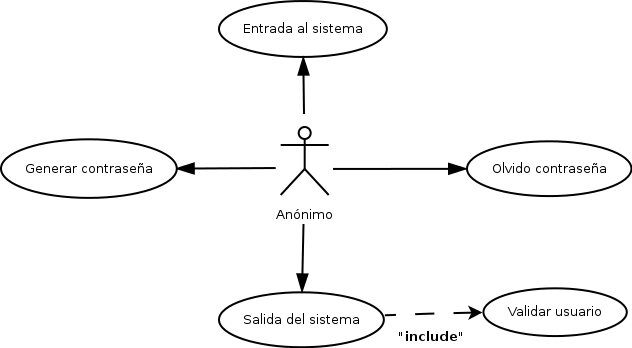
\includegraphics[scale=0.5]{login.png}
  \caption{Diagrama caso de uso. Gestión de entradas y salidas}
  \label{cu8}
\end{figure}
\smallskip
\hrule height 1pt
\smallskip
\textbf{Caso de uso: Entrada al sistema}
\begin{itemize}\renewcommand{\labelitemi}{$\cdot$}
  \item \textbf{Descripción:} El usuario introduce los datos para ingresar al sistema.
  \item \textbf{Actores:} Usuario
  \item \textbf{Postcondiciones:} El usuario ingresa en el sistema.
\end{itemize}
\underline{\textbf{Identificación de escenarios:}}
\begin{itemize}\renewcommand{\labelitemi}{$\circ$}
 \item \textbf{Escenario principal:}
         \begin{enumerate}
          \item El caso de uso se inicia cuando el usuario decide entrar en el sistema.
          \item El usuario introduce nombre de usuario y contraseña.
          \item El sistema comprueba que los datos introducidos son correctos.
	  \item El sistema almacena la entrada del usuario.
          \item El usuario entra en el sistema y se muestra la pantalla principal.
         \end{enumerate}
  \item \textbf{Escenario alternativos:}\\\\
		2a. El usuario no introduce la contraseña correcta.
  			\begin{enumerate}
  			\item El sistema muestra el error y pide nuevos datos.
  			\end{enumerate}
		2b. El usuario no introduce datos.
  			\begin{enumerate}
  			\item El sistema muestra el error y pide nuevos datos.
  			\end{enumerate}
          *a. El usuario cancela en cualquier momento la inserción al sistema.
\end{itemize}

\smallskip
\hrule height 1pt
\smallskip
\textbf{Caso de uso: Salida del sistema}
\begin{itemize}\renewcommand{\labelitemi}{$\cdot$}
 \item \textbf{Descripción:} El usuario decide salir del sistema.
  \item \textbf{Actores:} Usuario
  \item \textbf{Precondiciones:} Se debe comprobar que el usuario este autenticado en el sistema con el caso de uso Validar usuario.
  \item \textbf{Postcondiciones:} El sistema realiza la salida del usuario del sistema.
\end{itemize}
\underline{\textbf{Identificación de escenarios:}}
\begin{itemize}\renewcommand{\labelitemi}{$\circ$}
 \item \textbf{Escenario principal:}
         \begin{enumerate}
          \item El caso de uso se inicia cuando el usuario decide salir del sistema.
	 \item El sistema almacena la salida del sistema.
          \item El sistema facilita la salida del usuario del sistema.
	  \item El sistema muestra la pantalla principal de entrada al sistema.
         \end{enumerate}
\end{itemize}
\smallskip
\hrule height 1pt
\smallskip
\textbf{Caso de uso: Olvido de contraseña}
\begin{itemize}\renewcommand{\labelitemi}{$\cdot$}
 \item \textbf{Descripción:} El usuario decide recuperar su contraseña.
  \item \textbf{Actores:} Usuario.
  \item \textbf{Postcondiciones:} El sistema manda un email con un link para poder generar una nueva contraseña para el usuario.
\end{itemize}
\underline{\textbf{Identificación de escenarios:}}
\begin{itemize}\renewcommand{\labelitemi}{$\circ$}
 \item \textbf{Escenario principal:}
         \begin{enumerate}
          \item El caso de uso se inicia cuando el usuario decide recuperar su contraseña.
          \item El usuario introduce su email.
          \item El sistema comprueba que ese email pertenece a un cliente.
          \item El sistema manda un email con un link de generación de contraseña.
         \end{enumerate}
  \item \textbf{Escenario alternativos:}\\
  			3a. El email no pertenece a ningún usuario.
  			\begin{enumerate}
  			\item El sistema muestra el error y pide nuevo email.
  			\end{enumerate}
          *a. El usuario cancela en cualquier momento la recuperación de la contraseña.
\end{itemize}

\smallskip
\hrule height 1pt
\smallskip
\textbf{Caso de uso: Generar Contraseña}
\begin{itemize}\renewcommand{\labelitemi}{$\cdot$}
 \item \textbf{Descripción:} El usuario pulsa el link de generación de nueva contraseña.
  \item \textbf{Actores:} Usuario.
  \item \textbf{Postcondiciones:} El sistema almacena una nueva contraseña aleatoria para el usuario.
\end{itemize}
\underline{\textbf{Identificación de escenarios:}}
\begin{itemize}\renewcommand{\labelitemi}{$\circ$}
 \item \textbf{Escenario principal:}
         \begin{enumerate}
          \item El caso de uso se inicia cuando el usuario pulsa en el link de recuperación.
          \item El sistema comprueba que ese link es válido.
          \item El sistema genera una nueva contraseña y la manda por email al usuario.
         \end{enumerate}
  \item \textbf{Escenario alternativos:}\\
  			3a. El link no es válido.
  			\begin{enumerate}
  			\item El sistema muestra el error.
  			\end{enumerate}
\end{itemize}

\subsection{Requisito funcional: Estadísticas}

\begin{itemize}
 \item El usuario podrá ver sus propias estadísticas.
 \item El administrador podrá ver las estadísticas de la empresa.
 \item Se podrán exportar las estadísticas a distintos formatos.

\end{itemize}
\begin{figure}[H]
  \centering
    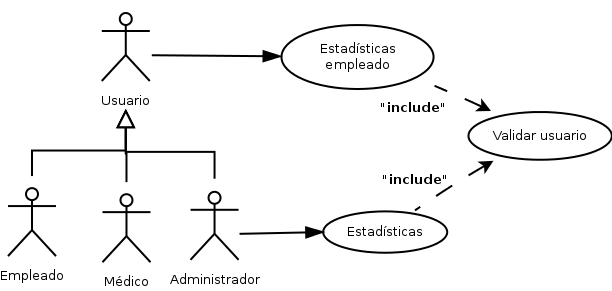
\includegraphics[scale=0.5]{estadisticas.png}
  \caption{Diagrama caso de uso. Estadisticas}
  \label{cu8}
\end{figure}
\smallskip
\hrule height 1pt
\smallskip
\textbf{Caso de uso: Estadisticas empleado}
\begin{itemize}\renewcommand{\labelitemi}{$\cdot$}
  \item \textbf{Descripción:} El usuario decide observar sus estadísticas.
  \item \textbf{Actores:} Usuario
  \item \textbf{Precondiciones:} Se debe comprobar que el usuario este autenticado en el sistema con el caso de uso Validar usuario.
  \item \textbf{Postcondiciones:} El sistema muestra por pantalla las distintas estadísticas del empleado.
\end{itemize}
\underline{\textbf{Identificación de escenarios:}}
\begin{itemize}\renewcommand{\labelitemi}{$\circ$}
 \item \textbf{Escenario principal:}
         \begin{enumerate}
          \item El caso de uso se inicia cuando el usuario decide consultar sus estadísticas.
          \item El sistema muestra por pantalla las estadísticas.
         \end{enumerate}
  \item \textbf{Escenario alternativos:}\\\\
          *a. El usuario cancela en cualquier momento la consulta de sus estadísticas.
\end{itemize}

\smallskip
\hrule height 1pt
\smallskip
\textbf{Caso de uso: Estadisticas}
\begin{itemize}\renewcommand{\labelitemi}{$\cdot$}
  \item \textbf{Descripción:} El administrador decide observar las estadísticas del sistema.
  \item \textbf{Actores:} Administrador
  \item \textbf{Precondiciones:} Se debe comprobar que el administrador este autenticado en el sistema con el caso de uso Validar usuario.
  \item \textbf{Postcondiciones:} El sistema muestra por pantalla las distintas estadísticas generadas.
\end{itemize}
\underline{\textbf{Identificación de escenarios:}}
\begin{itemize}\renewcommand{\labelitemi}{$\circ$}
 \item \textbf{Escenario principal:}
         \begin{enumerate}
          \item El caso de uso se inicia cuando el empleado decide consultar las estadísticas.
          \item El sistema muestra por pantalla las estadísticas del sistema.
         \end{enumerate}
  \item \textbf{Escenario alternativos:}\\\\
          *a. El administrador cancela en cualquier momento la consulta de las estadísticas del sistema.
\end{itemize}

\subsection{Requisito funcional: Gestión de pedidos}

\begin{itemize}
 \item El usuario podrá registrar un nuevo pedido a un proveedor.
 \item El usuario podrá consultar e imprimir el listado de todos los pedidos del sistema.
 \item El usuario podrá recepcionar la llegada de los pedidos.
 \item El usuario podrá ver los productos asociados al pedido.
 \item El usuario podrá realizar filtrados de los pedidos del sistema.
 \item El usuario podrá generar un documento de pedido.
\end{itemize}
\begin{figure}[H]
  \centering
    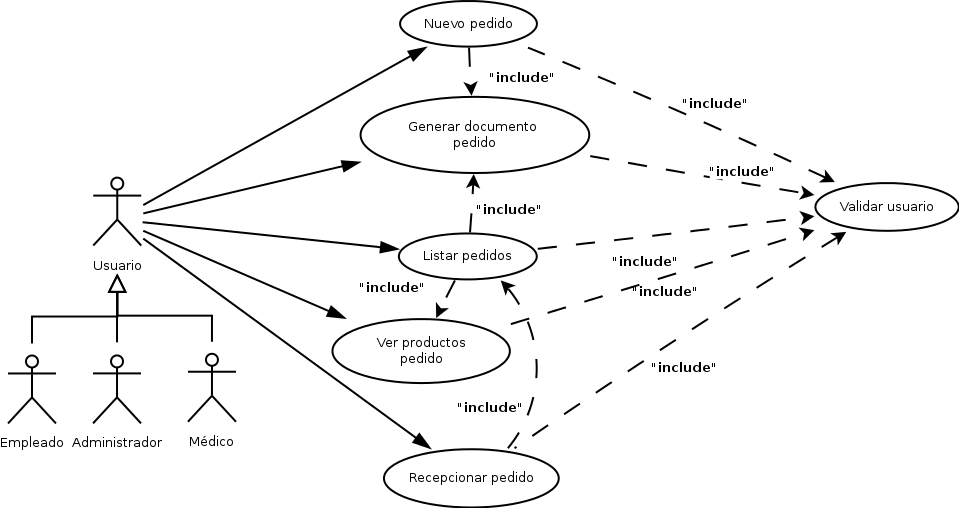
\includegraphics[scale=0.4]{gestionpedidos.png}
  \caption{Diagrama caso de uso. Gestión de pedidos}
  \label{cu1}
\end{figure}
\smallskip
\hrule height 1pt
\smallskip
\textbf{Caso de uso: Registrar pedido}
\begin{itemize}\renewcommand{\labelitemi}{$\cdot$}
 \item \textbf{Descripción:} El usuario introduce los datos para registrar un nuevo pedido en el sistema.
  \item \textbf{Actores:} Usuario
  \item \textbf{Precondiciones:} Se debe comprobar que el usuario este autenticado en el sistema con el caso de uso Validar usuario.
  \item \textbf{Postcondiciones:} El sistema almacena al pedido en el sistema.
\end{itemize}
\underline{\textbf{Identificación de escenarios:}}
\begin{itemize}\renewcommand{\labelitemi}{$\circ$}
 \item \textbf{Escenario principal:}
         \begin{enumerate}
          \item El caso de uso se inicia cuando el usuario decide registrar un nuevo pedido.
          \item El sistema muestra una lista de los proveedores para realizar el pedido.
          \item El usuario selecciona el proveedor para realizar el pedido.
         \item  El sistema muestra por pantalla los productos que suministra el proveedor.
          \item El usuario indica las cantidades y productos que desea añadir al pedido.
          \item El sistema comprueba que los datos introducidos son correctos. 
          \item El sistema muestra un mensaje de confirmación.
          \item El administrador pulsa SI en el mensaje de confirmación.
 	  \item El sistema almacena el cambio del sistema (auditoria).
          \item El pedido queda registrado en el sistema y el sistema muestra un mensaje de éxito.
         \end{enumerate}
  \item \textbf{Escenario alternativos:}\\\\
	6a. El usuario introduce de manera incorrecta los datos.
		\begin{enumerate}
		 \item El sistema muestra el error y pide que se introduzcan nuevos datos.
		\end{enumerate}
   	8a. El administrador decide no registrar un nuevo pedido
	      \begin{enumerate}
	       \item El sistema cancela el registro de un nuevo pedido y pide nuevos datos.
	      \end{enumerate}
          *a. El usuario cancela en cualquier momento el proceso de registro de un nuevo pedido.
\end{itemize}
\smallskip
\hrule height 1pt
\smallskip
\textbf{Caso de uso: Recepcionar pedido}
\begin{itemize}\renewcommand{\labelitemi}{$\cdot$}
 \item \textbf{Descripción:} El usuario recepciona un pedido en el sistema.
  \item \textbf{Actores:} Usuario
  \item \textbf{Precondiciones:} El pedido ya existe en el sistema. Se debe comprobar que el usuario este autenticado en el sistema con el caso de uso Validar usuario.
  \item \textbf{Postcondiciones:} El sistema recepciona el pedido en el sistema.
\end{itemize}
\underline{\textbf{Identificación de escenarios:}}
\begin{itemize}\renewcommand{\labelitemi}{$\circ$}
 \item \textbf{Escenario principal:}
         \begin{enumerate}
          \item El caso de uso se inicia cuando el usuario decide recepcionar un nuevo pedido.
          \item El sistema actualiza los stocks de los productos que han llegado en el pedido.
 	  \item El sistema almacena el cambio del sistema (auditoria).
          \item El sistema guarda los cambios.
       \end{enumerate}
\end{itemize}

\smallskip
\hrule height 1pt
\smallskip
\textbf{Caso de uso: Listar pedidos}
\begin{itemize}\renewcommand{\labelitemi}{$\cdot$}
 \item \textbf{Descripción:} El usuario decide consultar los pedidos en el sistema.
  \item \textbf{Actores:} Usuario
  \item \textbf{Precondiciones:} Se debe comprobar que el usuario este autenticado en el sistema con el caso de uso Validar usuario.
  \item \textbf{Postcondiciones:} El sistema muestra por pantalla todos los pedidos.
\end{itemize}
\underline{\textbf{Identificación de escenarios:}}
\begin{itemize}\renewcommand{\labelitemi}{$\circ$}
 \item \textbf{Escenario principal:}
         \begin{enumerate}
          \item El caso de uso se inicia cuando el usuario decide consultar todos los pedidos.
          \item El sistema muestra un listado de todos los pedidos.
          \item El usuario no selecciona un patrón de búsqueda.
          \item El sistema muestra todos los pedidos.
         \end{enumerate}
  \item \textbf{Escenario alternativos:}\\
  			3a. El usuario introduce un patrón de búsqueda.
  			\begin{enumerate}
  			\item El sistema muestra los datos acordes a ese patrón de búsqueda.
  			\item El usuario puede seleccionar el patrón de búsqueda cuantas veces desee.
  			\end{enumerate}
          *a. El usuario cancela en cualquier momento la consulta de los pedidos del sistema.
\end{itemize}

\smallskip
\hrule height 1pt
\smallskip
\textbf{Caso de uso: Generar documento pedido}
\begin{itemize}\renewcommand{\labelitemi}{$\cdot$}
 \item \textbf{Descripción:} El usuario decide generar el documento de pedido.
  \item \textbf{Actores:} Usuario
  \item \textbf{Precondiciones:} Se debe comprobar que el usuario este autenticado en el sistema con el caso de uso Validar usuario.
  \item \textbf{Postcondiciones:} El sistema muestra por pantalla el documento generado.
\end{itemize}
\underline{\textbf{Identificación de escenarios:}}
\begin{itemize}\renewcommand{\labelitemi}{$\circ$}
 \item \textbf{Escenario principal:}
         \begin{enumerate}
          \item El caso de uso se inicia cuando el usuario decide generar el documento.
          \item El sistema muestra por pantalla el documento de pedido generado.
         \end{enumerate}
\end{itemize}

\smallskip
\hrule height 1pt
\smallskip
\textbf{Caso de uso: Ver productos pedido}
\begin{itemize}\renewcommand{\labelitemi}{$\cdot$}
 \item \textbf{Descripción:} El usuario decide consultar los productos del pedido.
  \item \textbf{Actores:} Usuario
  \item \textbf{Precondiciones:} Se debe comprobar que el usuario este autenticado en el sistema con el caso de uso Validar usuario.
  \item \textbf{Postcondiciones:} El sistema muestra por pantalla todos los productos del pedido.
\end{itemize}
\underline{\textbf{Identificación de escenarios:}}
\begin{itemize}\renewcommand{\labelitemi}{$\circ$}
 \item \textbf{Escenario principal:}
         \begin{enumerate}
          \item El caso de uso se inicia cuando el usuario decide consultar los productos del pedido.
          \item El sistema muestra todos los productos del pedido.
         \end{enumerate}
\end{itemize}

\subsection{Requisito funcional: Gestión de arqueos}

\begin{itemize}
 \item El usuario podrá registrar un nuevo arqueo en el sistema.
 \item El administrador podrá consultar e imprimir el listado de todos los arqueos del sistema.
\end{itemize}
\begin{figure}[H]
  \centering
    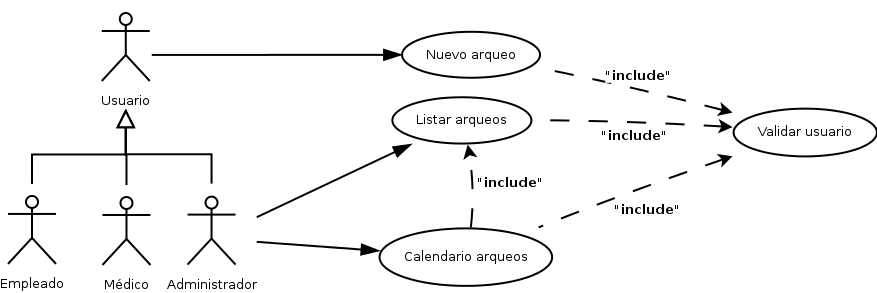
\includegraphics[scale=0.4]{gestionararqueos.png}
  \caption{Diagrama caso de uso. Gestión de arqueos}
  \label{cu1}
\end{figure}
\smallskip
\hrule height 1pt
\smallskip
\textbf{Caso de uso: Nuevo arqueo}
\begin{itemize}\renewcommand{\labelitemi}{$\cdot$}
 \item \textbf{Descripción:} El usuario registra un nuevo arqueo en el sistema.
  \item \textbf{Actores:} Usuario
  \item \textbf{Precondiciones:} Se debe comprobar que en esa fecha no exista un arqueo. Se debe comprobar que el usuario este autenticado en el sistema con el caso de uso Validar usuario.
  \item \textbf{Postcondiciones:} El sistema almacena el arqueo en el sistema.
\end{itemize}
\underline{\textbf{Identificación de escenarios:}}
\begin{itemize}\renewcommand{\labelitemi}{$\circ$}
 \item \textbf{Escenario principal:}
         \begin{enumerate}
          \item El caso de uso se inicia cuando el usuario decide registrar un nuevo arqueo en el sistema.
	\item El sistema muestra la pantalla para la selección de monedas, billetes y boletas.
	   \item El sistema comprueba que los datos introducidos son válidos.
	\item El sistema comprueba que el arqueo es correcto.
 	  \item El sistema almacena el cambio del sistema (auditoria).
          \item El arqueo queda registrado en el sistema.
         \end{enumerate}
  \item \textbf{Escenario alternativos:}\\\\
	4a. El usuario introduce de manera incorrecta los datos.
		\begin{enumerate}
		 \item El sistema muestra el error y pide que se introduzcan de nuevo los datos.
		\end{enumerate}
	5a. El usuario introduce un arqueo inválido.
		\begin{enumerate}
		 \item El sistema muestra el error y da la opción a intentarlo de nuevo o guardar el arqueo inválido.
		\end{enumerate}
          *a. El usuario cancela en cualquier momento el proceso de registro de un nuevo arqueo.
\end{itemize}

\smallskip
\hrule height 1pt
\smallskip
\textbf{Caso de uso: Calendario arqueos}
\begin{itemize}\renewcommand{\labelitemi}{$\cdot$}
 \item \textbf{Descripción:} El administrador decide mostrar el calendario de arqueos.
  \item \textbf{Actores:} Administrador
  \item \textbf{Precondiciones:} Se debe comprobar que el administrador este autenticado en el sistema con el caso de uso Validar usuario.
  \item \textbf{Postcondiciones:} El sistema muestra el calendario con todos los arqueos almacenados en el sistema.
\end{itemize}
\underline{\textbf{Identificación de escenarios:}}
\begin{itemize}\renewcommand{\labelitemi}{$\circ$}
 \item \textbf{Escenario principal:}
         \begin{enumerate}
          \item El caso de uso se inicia cuando el administrador decide mostrar el calendario de arqueos.
	  \item El sistema muestra por pantalla todos los arqueos en el calendario.
         \end{enumerate}
\end{itemize}

\smallskip
\hrule height 1pt
\smallskip
\textbf{Caso de uso: Listar arqueos}
\begin{itemize}\renewcommand{\labelitemi}{$\cdot$}
 \item \textbf{Descripción:} El administrador decide consultar los permisos en el sistema.
  \item \textbf{Actores:} Administrador
  \item \textbf{Precondiciones:} Se debe comprobar que el administrador este autenticado en el sistema con el caso de uso Validar usuario.
  \item \textbf{Postcondiciones:} El sistema muestra por pantalla todos los arqueos.
\end{itemize}
\underline{\textbf{Identificación de escenarios:}}
\begin{itemize}\renewcommand{\labelitemi}{$\circ$}
 \item \textbf{Escenario principal:}
         \begin{enumerate}
          \item El caso de uso se inicia cuando el administrador decide consultar todos los arqueos.
          \item El sistema muestra un listado de todos los arqueos.
          \item El usuario no selecciona un patrón de búsqueda.
          \item El sistema muestra todos los permisos.
         \end{enumerate}
  \item \textbf{Escenario alternativos:}\\
  			3a. El usuario introduce un patrón de búsqueda.
  			\begin{enumerate}
  			\item El sistema muestra los datos acordes a ese patrón de búsqueda.
  			\item El administrador puede seleccionar el patrón de búsqueda cuantas veces desee.
  			\end{enumerate}
          *a. El administrador cancela en cualquier momento la consulta de los arqueos del sistema.
\end{itemize}

\subsection{Requisito funcional: Gestión de permisos}

\begin{itemize}
 \item El administrador podrá registrar un nuevo permiso en el sistema.
 \item El administrador podrá consultar e imprimir el listado de todos los permisos del sistema.
 \item El administrador podrá modificar los permisos del sistema.
 \item El administrador podrá eliminar un permiso en concreto del sistema.
 \item El administrador podrá realizar filtrados de los permisos del sistema.
 \item El usuario podrá consultar sus permisos.
\end{itemize}
\begin{figure}[H]
  \centering
    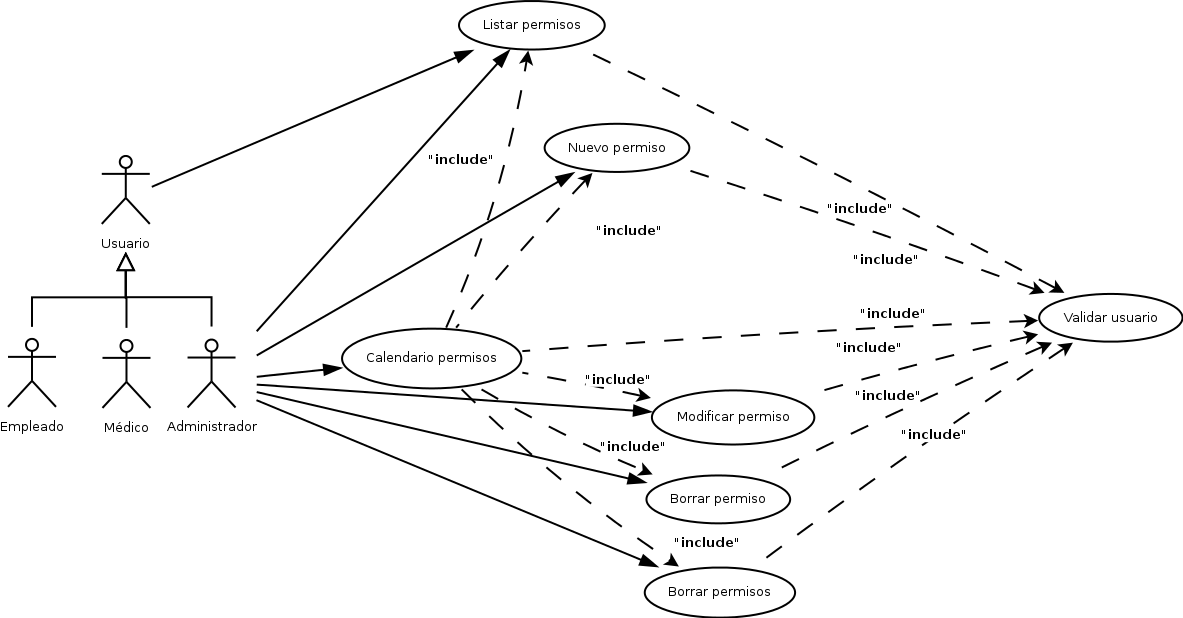
\includegraphics[scale=0.4]{gestionpermisos.png}
  \caption{Diagrama caso de uso. Gestión de permisos}
  \label{cu1}
\end{figure}
\smallskip
\hrule height 1pt
\smallskip
\textbf{Caso de uso: Nuevo permiso}
\begin{itemize}\renewcommand{\labelitemi}{$\cdot$}
 \item \textbf{Descripción:} El empleado registra un nuevo permiso en el sistema.
  \item \textbf{Actores:} Administrador 
  \item \textbf{Precondiciones:} Se debe comprobar que el administrador este autenticado en el sistema con el caso de uso Validar usuario.
  \item \textbf{Postcondiciones:} El sistema almacena el permiso en el sistema.
\end{itemize}
\underline{\textbf{Identificación de escenarios:}}
\begin{itemize}\renewcommand{\labelitemi}{$\circ$}
 \item \textbf{Escenario principal:}
         \begin{enumerate}
          \item El caso de uso se inicia cuando el administrador decide registrar un nuevo permiso en el sistema.
          \item El administrador arrastra al usuario a la fecha del permiso.
	   \item El sistema comprueba que el permiso sea válido.
 	  \item El sistema almacena el cambio del sistema (auditoria).
          \item El permiso queda registrado en el sistema y el permiso aparece en el calendario.
         \end{enumerate}
  \item \textbf{Escenario alternativos:}\\\\
	3a. El aministrador introduce un permiso inválido.
		\begin{enumerate}
		 \item El sistema muestra el error y cancela el registro del permiso.
		\end{enumerate}
          *a. El administrador cancela en cualquier momento el proceso de registro de un nuevo permiso.
\end{itemize}

\smallskip
\hrule height 1pt
\smallskip
\textbf{Caso de uso: Borrar permiso}
\begin{itemize}\renewcommand{\labelitemi}{$\cdot$}
 \item \textbf{Descripción:} El administrador elimina un permiso en concreto en el sistema.
  \item \textbf{Actores:} Administrador 
  \item \textbf{Precondiciones:} Se debe comprobar que el administrador este autenticado en el sistema con el caso de uso Validar usuario.
  \item \textbf{Postcondiciones:} El sistema almacena el permiso modificado en el sistema.
\end{itemize}
\underline{\textbf{Identificación de escenarios:}}
\begin{itemize}\renewcommand{\labelitemi}{$\circ$}
 \item \textbf{Escenario principal:}
         \begin{enumerate}
          \item El caso de uso se inicia cuando el administrador decide eliminar un permiso en el sistema.
	  \item El administrador pulsa en el permiso que desea eliminar.
	  \item El sistema muestra un mensaje de confirmación.
          \item El administrador pulsa SI en el mensaje de confirmación.
 	  \item El sistema almacena el cambio del sistema (auditoria).
          \item El permiso queda eliminado en el sistema y el permiso aparece en el calendario.
         \end{enumerate}
  \item \textbf{Escenario alternativos:}\\\\
		4a. El administrador decide no borrar el permiso.
  			\begin{enumerate}
  			\item El sistema cancela el proceso de eliminación de un permiso.
  			\end{enumerate}
          *a. El administrador cancela en cualquier momento el proceso de eliminación del permiso.
\end{itemize}

\smallskip
\hrule height 1pt
\smallskip
\textbf{Caso de uso: Borrar permisos}
\begin{itemize}\renewcommand{\labelitemi}{$\cdot$}
 \item \textbf{Descripción:} El administrador elimina los permisos de un determinado tipo en concreto en el sistema.
  \item \textbf{Actores:} Administrador 
  \item \textbf{Precondiciones:} Se debe comprobar que el administrador este autenticado en el sistema con el caso de uso Validar usuario.
  \item \textbf{Postcondiciones:} El sistema elimina los permisos de ese tipo en el sistema.
\end{itemize}
\underline{\textbf{Identificación de escenarios:}}
\begin{itemize}\renewcommand{\labelitemi}{$\circ$}
 \item \textbf{Escenario principal:}
         \begin{enumerate}
          \item El caso de uso se inicia cuando el administrador decide eliminar los permisos de un tipo en el sistema.
	  \item El administrador pulsa en el tipo de permiso que desea eliminar.
	  \item El sistema muestra un mensaje de confirmación.
          \item El administrador pulsa SI en el mensaje de confirmación.
 	  \item El sistema almacena el cambio del sistema (auditoria).
          \item Los permisos quedan eliminados en el sistema y el permiso aparece en el calendario.
         \end{enumerate}
  \item \textbf{Escenario alternativos:}\\\\
		4a. El administrador decide no borrar los permisos.
  			\begin{enumerate}
  			\item El sistema cancela el proceso de eliminación de los permisos.
  			\end{enumerate}
          *a. El administrador cancela en cualquier momento el proceso de eliminación de los permisos.
\end{itemize}

\smallskip
\hrule height 1pt
\smallskip
\textbf{Caso de uso: Calendario permisos}
\begin{itemize}\renewcommand{\labelitemi}{$\cdot$}
 \item \textbf{Descripción:} El administrador decide mostrar el calendario de permisos.
  \item \textbf{Actores:} Administrador
  \item \textbf{Precondiciones:} Se debe comprobar que el administrador este autenticado en el sistema con el caso de uso Validar usuario.
  \item \textbf{Postcondiciones:} El sistema muestra el calendario con todos los permisos almacenados en el sistema.
\end{itemize}
\underline{\textbf{Identificación de escenarios:}}
\begin{itemize}\renewcommand{\labelitemi}{$\circ$}
 \item \textbf{Escenario principal:}
         \begin{enumerate}
          \item El caso de uso se inicia cuando el administrador decide mostrar el calendario de permisos.
	  \item El sistema muestra por pantalla todos los permisos en el calendario.
         \end{enumerate}
\end{itemize}

\smallskip
\hrule height 1pt
\smallskip
\textbf{Caso de uso: Listar permisos}
\begin{itemize}\renewcommand{\labelitemi}{$\cdot$}
 \item \textbf{Descripción:} El administrador decide consultar los permisos en el sistema.
  \item \textbf{Actores:} Administrador, Cliente
  \item \textbf{Precondiciones:} Se debe comprobar que el administrador este autenticado en el sistema con el caso de uso Validar usuario. Si el usuario no es administrador sólo podrá listar sus propios permisos.
  \item \textbf{Postcondiciones:} El sistema muestra por pantalla todos los permisos.
\end{itemize}
\underline{\textbf{Identificación de escenarios:}}
\begin{itemize}\renewcommand{\labelitemi}{$\circ$}
 \item \textbf{Escenario principal:}
         \begin{enumerate}
          \item El caso de uso se inicia cuando el administrador decide consultar todos los permisos.
          \item El sistema muestra un listado de todos los permisos.
          \item El usuario no selecciona un patrón de búsqueda.
          \item El sistema muestra todos los permisos.
         \end{enumerate}
  \item \textbf{Escenario alternativos:}\\
  			3a. El administrador introduce un patrón de búsqueda.
  			\begin{enumerate}
  			\item El sistema muestra los datos acordes a ese patrón de búsqueda.
  			\item El administrador puede seleccionar el patrón de búsqueda cuantas veces desee.
  			\end{enumerate}
          *a. El usuario cancela en cualquier momento la consulta de los permisos del sistema.
\end{itemize}

\section{Requisitos de información}

En este apartado estudiaremos todos los datos referentes al diseño del esquema conceptual: Se identificarán las clases, atributos, relaciones, restricciones adicionales y reglas de derivación necesarias.

\clearpage

\subsection{Modelo conceptual de datos}
\begin{figure}[H]
  \centering
    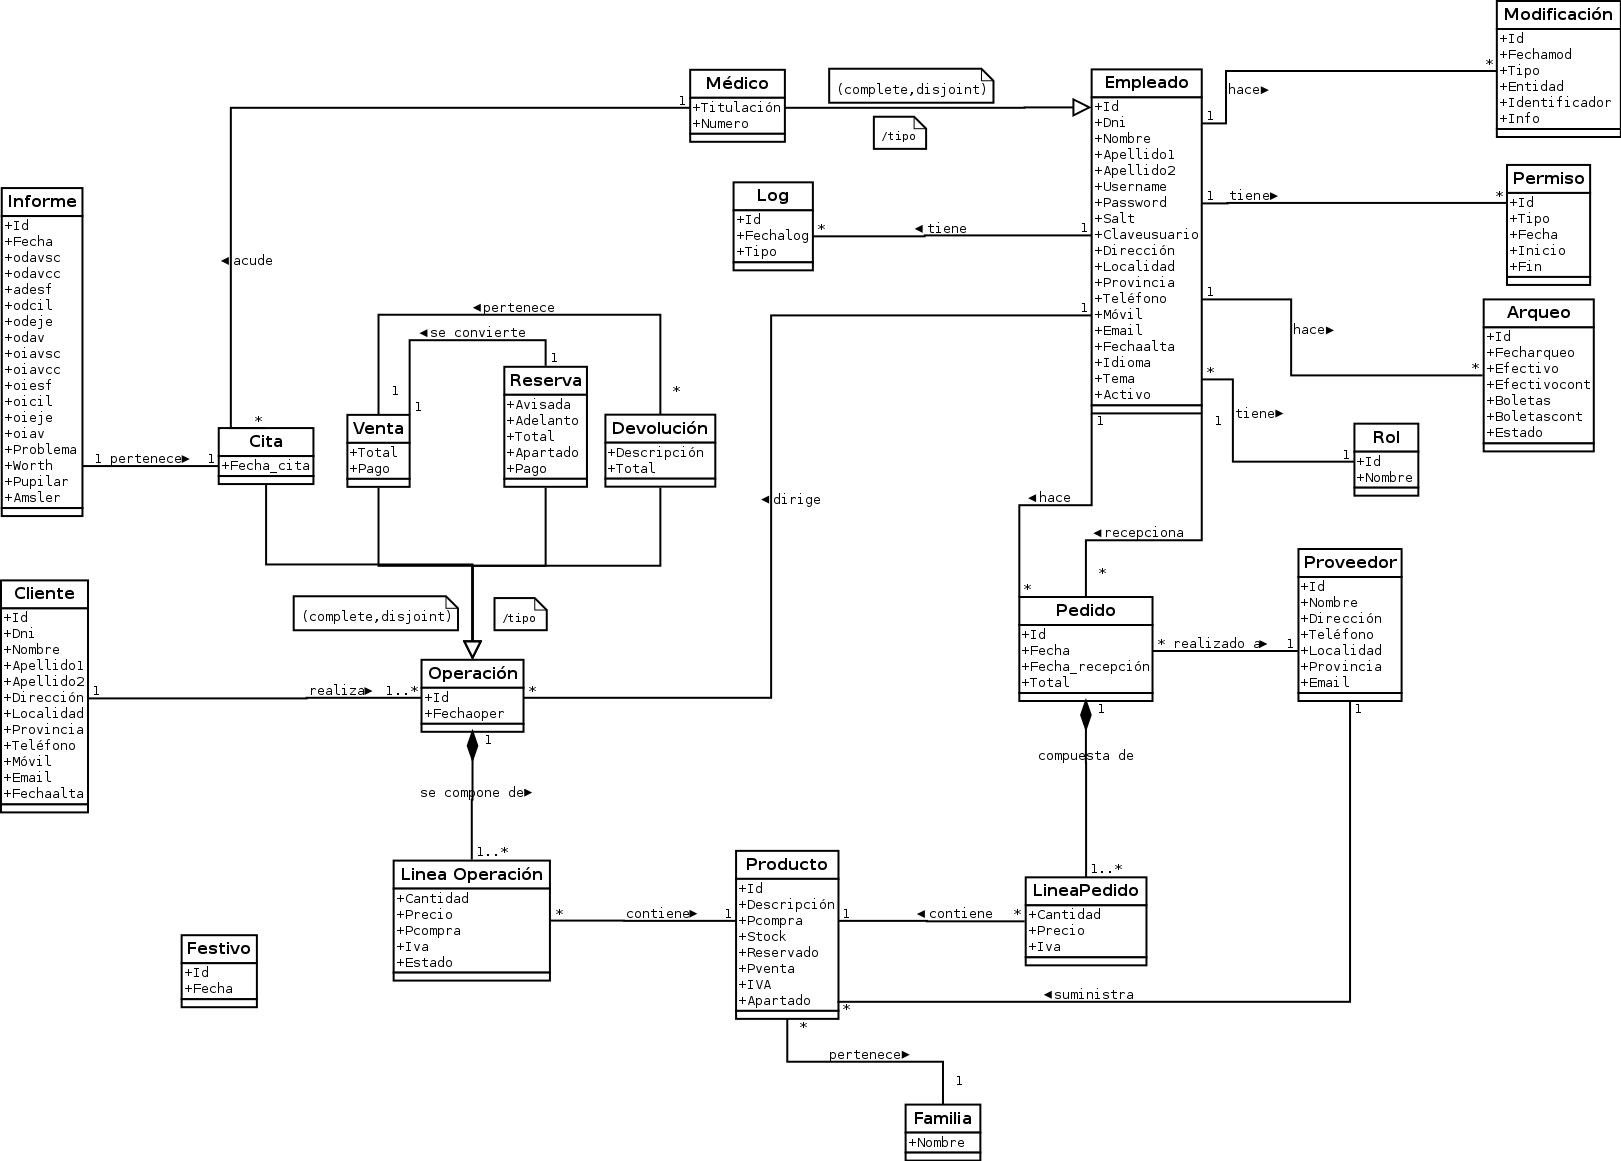
\includegraphics[angle=-90,scale=0.34]{UML.png}
  \caption{Modelo conceptual de datos.}
  \label{uml}
\end{figure}

\section{Modelo comportamiento del sistema}

\subsection{Diagramas de secuencia de sistemas}

Una vez descritos los casos de uso, nos ponemos manos a la obra para realizar los diferentes diagramas de secuencia. En esta fase de análisis describiremos los diagramas de manera muy simplificada ya que estos se estudiarán más a fondo en la fase de diseño.\\
Sólo nos centraremos en los diagramas que tengan relevancia ya que muchos de ellos son muy similares.

\subsubsection{Gestión de entradas y salidas del sistema}
\begin{figure}[!htb]
  \centering
    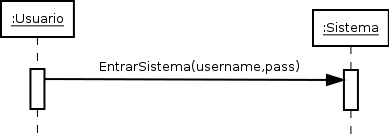
\includegraphics[scale=0.5]{aentrarsistema.png}
  \caption{Diagrama de secuencia - Caso de uso: Entrada al sistema }
  \label{a}
\end{figure}

\begin{figure}[!htb]
  \centering
    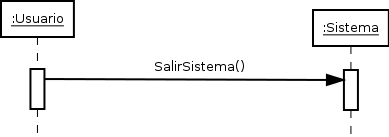
\includegraphics[scale=0.5]{asalirsistema.png}
  \caption{Diagrama de secuencia - Caso de uso: Salida del sistema }
  \label{a}
\end{figure}

\begin{figure}[!htb]
  \centering
    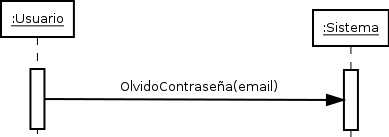
\includegraphics[scale=0.5]{aolvidocontrasena.png}
  \caption{Diagrama de secuencia - Caso de uso: Olvido contraseña  }
  \label{a}
\end{figure}

\begin{figure}[!htb]
  \centering
    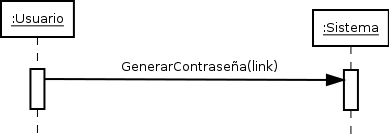
\includegraphics[scale=0.5]{agenerarcontrasena.png}
  \caption{Diagrama de secuencia - Caso de uso: Generar contraseña  }
  \label{a}
\end{figure}

\clearpage
\subsubsection{Gestión de clientes}
\begin{figure}[!htb]
  \centering
    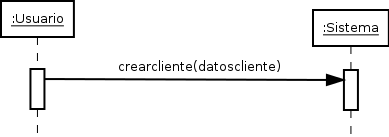
\includegraphics[scale=0.5]{aregistrarcliente.png}
  \caption{Diagrama de secuencia - Caso de uso: Registrar cliente }
  \label{a}
\end{figure}

\begin{figure}[!htb]
  \centering
    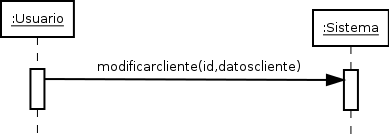
\includegraphics[scale=0.5]{aeditarcliente.png}
  \caption{Diagrama de secuencia - Caso de uso: Modificar cliente }
  \label{a}
\end{figure}

\begin{figure}[!htb]
  \centering
    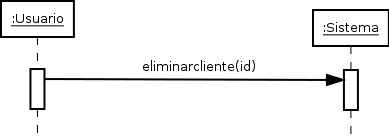
\includegraphics[scale=0.5]{aborrarcliente.png}
  \caption{Diagrama de secuencia - Caso de uso: Borrar cliente   }
  \label{a}
\end{figure}

\begin{figure}[!htb]
  \centering
    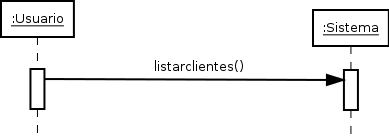
\includegraphics[scale=0.5]{acliente.png}
  \caption{Diagrama de secuencia - Caso de uso: Listar clientes   }
  \label{a}
\end{figure}

\begin{figure}[!htb]
  \centering
    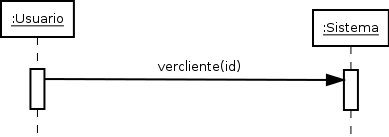
\includegraphics[scale=0.5]{avercliente.png}
  \caption{Diagrama de secuencia - Caso de uso: Ver cliente   }
  \label{a}
\end{figure}

\vspace{15mm}
\subsubsection{Gestión de ventas}
\begin{figure}[!htb]
  \centering
    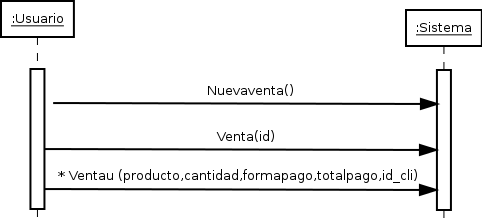
\includegraphics[scale=0.5]{aregistarventa.png}
  \caption{Diagrama de secuencia - Caso de uso: Nueva venta }
  \label{a}
\end{figure}

\begin{figure}[!htb]
  \centering
    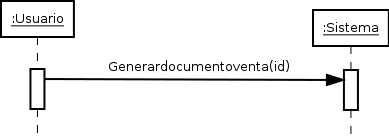
\includegraphics[scale=0.5]{agenerarfactura.png}
  \caption{Diagrama de secuencia - Caso de uso: Generar documento venta }
  \label{a}
\end{figure}

\begin{figure}[!htb]
  \centering
    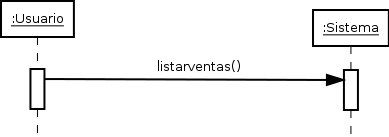
\includegraphics[scale=0.5]{aventa.png}
  \caption{Diagrama de secuencia - Caso de uso: Listar ventas   }
  \label{a}
\end{figure}

\begin{figure}[!htb]
  \centering
    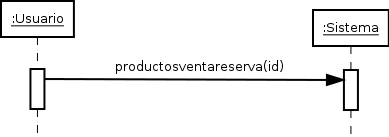
\includegraphics[scale=0.5]{averproductosventa.png}
  \caption{Diagrama de secuencia - Caso de uso: Ver productos venta }
  \label{a}
\end{figure}

\newpage
\subsubsection{Gestión de devoluciones}
\begin{figure}[!htb]
  \centering
    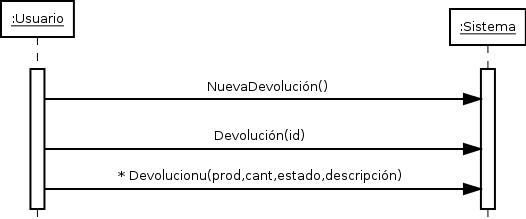
\includegraphics[scale=0.5]{aregistardevolucion.png}
  \caption{Diagrama de secuencia - Caso de uso: Nueva devolución }
  \label{a}
\end{figure}

\begin{figure}[!htb]
  \centering
    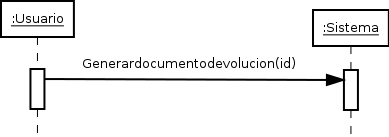
\includegraphics[scale=0.5]{agenerardocumento.png}
  \caption{Diagrama de secuencia - Caso de uso: Generar documento devolución}
  \label{a}
\end{figure}

\begin{figure}[!htb]
  \centering
    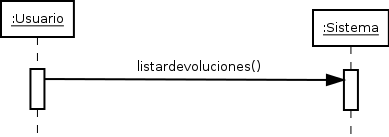
\includegraphics[scale=0.5]{adevolucion.png}
  \caption{Diagrama de secuencia - Caso de uso: Listar devoluciones }
  \label{a}
\end{figure}

\begin{figure}[!htb]
  \centering
    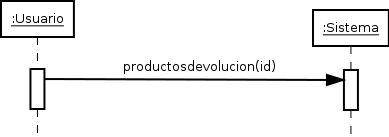
\includegraphics[scale=0.5]{averproductosdevueltos.png}
  \caption{Diagrama de secuencia - Caso de uso: Ver productos devolución  }
  \label{a}
\end{figure}

\newpage
\subsubsection{Gestión de reservas}
\begin{figure}[!htb]
  \centering
    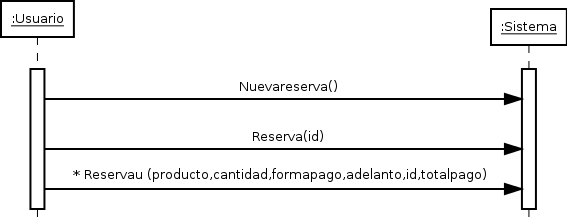
\includegraphics[scale=0.5]{aregistarreserva.png}
  \caption{Diagrama de secuencia - Caso de uso: Nueva reserva }
  \label{a}
\end{figure}

\begin{figure}[!htb]
  \centering
    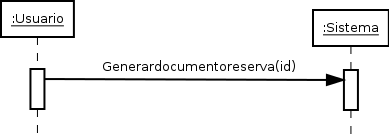
\includegraphics[scale=0.5]{agenerardocumentoreserva.png}
  \caption{Diagrama de secuencia - Caso de uso: Generar documento reserva }
  \label{a}
\end{figure}

\begin{figure}[!htb]
  \centering
    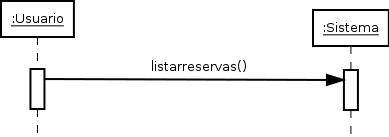
\includegraphics[scale=0.5]{areserva.png}
  \caption{Diagrama de secuencia - Caso de uso: Listar reservas   }
  \label{a}
\end{figure}

\begin{figure}[!htb]
  \centering
    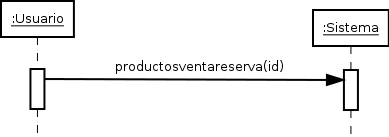
\includegraphics[scale=0.5]{averproductosreserva.png}
  \caption{Diagrama de secuencia - Caso de uso: Ver productos reserva  }
  \label{a}
\end{figure}

\begin{figure}[!htb]
  \centering
    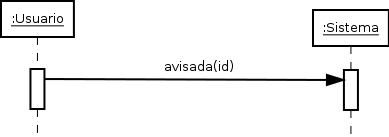
\includegraphics[scale=0.5]{aavisada.png}
  \caption{Diagrama de secuencia - Caso de uso: Avisar reserva   }
  \label{a}
\end{figure}

\begin{figure}[!htb]
  \centering
    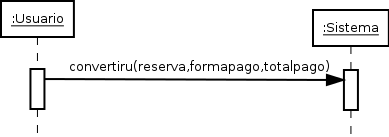
\includegraphics[scale=0.5]{aconvertir.png}
  \caption{Diagrama de secuencia - Caso de uso: Convertir a venta  }
  \label{a}
\end{figure}

\newpage
\subsubsection{Gestión de citas e informes}
\begin{figure}[!htb]
  \centering
    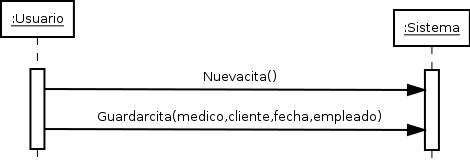
\includegraphics[scale=0.5]{aregistrarcita.png}
  \caption{Diagrama de secuencia - Caso de uso: Nueva cita }
  \label{a}
\end{figure}

\begin{figure}[!htb]
  \centering
    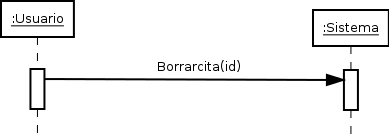
\includegraphics[scale=0.5]{aborrarcita.png}
  \caption{Diagrama de secuencia - Caso de uso: Borrar cita   }
  \label{a}
\end{figure}

\begin{figure}[!htb]
  \centering
    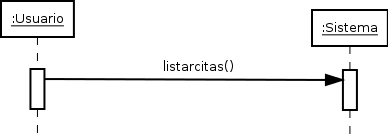
\includegraphics[scale=0.5]{acita.png}
  \caption{Diagrama de secuencia - Caso de uso: Listar citas   }
  \label{a}
\end{figure}

\begin{figure}[!htb]
  \centering
    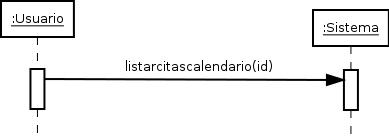
\includegraphics[scale=0.5]{acitas.png}
  \caption{Diagrama de secuencia - Caso de uso: Calendario citas   }
  \label{a}
\end{figure}

\begin{figure}[!htb]
  \centering
    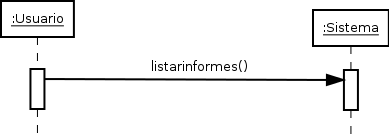
\includegraphics[scale=0.5]{ainforme.png}
  \caption{Diagrama de secuencia - Caso de uso: Listar informes   }
  \label{a}
\end{figure}

\begin{figure}[!htb]
  \centering
    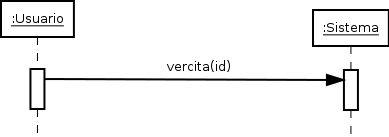
\includegraphics[scale=0.5]{avercita.png}
  \caption{Diagrama de secuencia - Caso de uso: Ver cita   }
  \label{a}
\end{figure}

\begin{figure}[!htb]
  \centering
    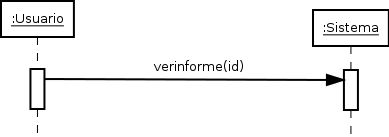
\includegraphics[scale=0.5]{averinforme.png}
  \caption{Diagrama de secuencia - Caso de uso: Ver informe   }
  \label{a}
\end{figure}

\begin{figure}[!htb]
  \centering
    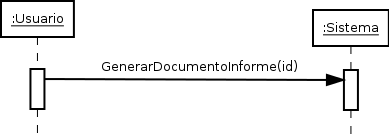
\includegraphics[scale=0.5]{agenerardocumentoinforme.png}
  \caption{Diagrama de secuencia - Caso de uso: Generar documento informe   }
  \label{a}
\end{figure}

\begin{figure}[!htb]
  \centering
    \includegraphics[scale=0.5]{agenerarinformeconcita.png}
  \caption{Diagrama de secuencia - Caso de uso: Nuevo informe con cita   }
  \label{a}
\end{figure}

\begin{figure}[!htb]
  \centering
    \includegraphics[scale=0.5]{agenerarinformesincita.png}
  \caption{Diagrama de secuencia - Caso de uso: Nuevo informe sin cita  }
  \label{a}
\end{figure}

\clearpage
\subsubsection{Gestión de pedidos}
\begin{figure}[!htb]
  \centering
    \includegraphics[scale=0.5]{aregistrarpedido.png}
  \caption{Diagrama de secuencia - Caso de uso: Nuevo pedido }
  \label{a}
\end{figure}

\begin{figure}[!htb]
  \centering
    \includegraphics[scale=0.5]{agenerardocumentopedido.png}
  \caption{Diagrama de secuencia - Caso de uso: Generar documento pedido }
  \label{a}
\end{figure}

\begin{figure}[!htb]
  \centering
    \includegraphics[scale=0.5]{apedido.png}
  \caption{Diagrama de secuencia - Caso de uso: Listar pedidos }
  \label{a}
\end{figure}

\begin{figure}[!htb]
  \centering
    \includegraphics[scale=0.5]{averproductospedido.png}
  \caption{Diagrama de secuencia - Caso de uso: Ver productos pedido }
  \label{a}
\end{figure}

\begin{figure}[!htb]
  \centering
    \includegraphics[scale=0.5]{arecepcionarpedido.png}
  \caption{Diagrama de secuencia - Caso de uso: Recepcionar pedido }
  \label{a}
\end{figure}

\subsubsection{Gestión de usuarios}
Se han omitido algunos diagramas ya que son similares a los anteriores.

\begin{figure}[!htb]
  \centering
    \includegraphics[scale=0.5]{aregistrarempleado.png}
  \caption{Diagrama de secuencia - Caso de uso: Registrar empleado  }
  \label{a}
\end{figure}

\begin{figure}[!htb]
  \centering
    \includegraphics[scale=0.5]{aregistrarmedico.png}
  \caption{Diagrama de secuencia - Caso de uso: Registrar médico   }
  \label{a}
\end{figure}

\begin{figure}[!htb]
  \centering
    \includegraphics[scale=0.5]{averconexiones.png}
  \caption{Diagrama de secuencia - Caso de uso: Listar conexiones   }
  \label{a}
\end{figure}

\begin{figure}[!htb]
  \centering
    \includegraphics[scale=0.5]{avercambios.png}
  \caption{Diagrama de secuencia - Caso de uso: Listar cambios  }
  \label{a}
\end{figure}
 
\clearpage
\subsubsection{Gestión de permisos}
\begin{figure}[!htb]
  \centering
    \includegraphics[scale=0.5]{aregistrarpermiso.png}
  \caption{Diagrama de secuencia - Caso de uso: Nuevo permiso }
  \label{a}
\end{figure}

\begin{figure}[!htb]
  \centering
    \includegraphics[scale=0.5]{aborrarpermiso.png}
  \caption{Diagrama de secuencia - Caso de uso: Borrar permiso }
  \label{a}
\end{figure}

\begin{figure}[!htb]
  \centering
    \includegraphics[scale=0.5]{aborrarpermisos.png}
  \caption{Diagrama de secuencia - Caso de uso: Borrar permisos }
  \label{a}
\end{figure}

\begin{figure}[!htb]
  \centering
    \includegraphics[scale=0.5]{amodificarpermiso.png}
  \caption{Diagrama de secuencia - Caso de uso: Modificar permiso }
  \label{a}
\end{figure}

\begin{figure}[!htb]
  \centering
    \includegraphics[scale=0.5]{alistarpermisos.png}
  \caption{Diagrama de secuencia - Caso de uso: Listar permisos }
  \label{a}
\end{figure}

\clearpage

\begin{figure}[!htb]
  \centering
    \includegraphics[scale=0.5]{acalendariopermisos.png}
  \caption{Diagrama de secuencia - Caso de uso: Calendario permisos }
  \label{a}
\end{figure}

\subsubsection{Gestión de festivos}
\begin{figure}[!htb]
  \centering
    \includegraphics[scale=0.5]{aregistrarfestivo.png}
  \caption{Diagrama de secuencia - Caso de uso: Registrar festivo }
  \label{a}
\end{figure}

\begin{figure}[!htb]
  \centering
    \includegraphics[scale=0.5]{aborrarfestivo.png}
  \caption{Diagrama de secuencia - Caso de uso: Borrar festivo }
  \label{a}
\end{figure}

\begin{figure}[!htb]
  \centering
    \includegraphics[scale=0.5]{afestivo.png}
  \caption{Diagrama de secuencia - Caso de uso: Listar festivos }
  \label{a}
\end{figure}

\begin{figure}[!htb]
  \centering
    \includegraphics[scale=0.5]{afestivos.png}
  \caption{Diagrama de secuencia - Caso de uso: Calendario festivos }
  \label{a}
\end{figure}
\clearpage

\subsubsection{Gestión de arqueos}
\begin{figure}[!htb]
  \centering
    \includegraphics[scale=0.5]{anuevoarqueo.png}
  \caption{Diagrama de secuencia - Caso de uso: Nuevo arqueo }
  \label{a}
\end{figure}

\begin{figure}[!htb]
  \centering
    \includegraphics[scale=0.5]{aarqueos.png}
  \caption{Diagrama de secuencia - Caso de uso: Listar arqueos }
  \label{a}
\end{figure}

\begin{figure}[!htb]
  \centering
    \includegraphics[scale=0.5]{aarqueoscalendario.png}
  \caption{Diagrama de secuencia - Caso de uso: Calendario arqueos }
  \label{a}
\end{figure}

\subsubsection{Estadísticas}
\begin{figure}[!htb]
  \centering
    \includegraphics[scale=0.5]{aestadistica.png}
  \caption{Diagrama de secuencia - Caso de uso: Estadísticas }
  \label{a}
\end{figure}

\begin{figure}[!htb]
  \centering
    \includegraphics[scale=0.5]{aestadistica1.png}
  \caption{Diagrama de secuencia - Caso de uso: Estadísticas empleado }
  \label{a}
\end{figure}

\newpage
\subsection{Contratos de las operaciones}

En este apartado describiremos el comportamiento que debe tener el sistema para cada diagrama descrito anteriormente. Sólo nos centraremos en lo que hace el sistema en cada operación pero no como lo hace. Para que no existan confusiones entre datos del sistema y datos proporcionados usaremos la notación W para datos proporcionados al sistema. Describiremos los contratos de las operaciones de forma clara haciendo uso de la siguiente plantilla estudiada en ingeniería del software:

\begin{table}[h]
\begin{tabular}{|m{6.0cm}|m{10.0cm}|}
\hline\hline                        %inserts double horizontal lines
\multicolumn{2}{|>{\columncolor[gray]{0.93}}c|}{\textbf{Plantilla de un contrato}  } \\
\hline
\hline                  % inserts single horizontal line
\textbf{Nombre operación} & Signatura de la operación \\ % inserting body of the table
\hline
\textbf{Responsabilidades} & Descripción informal del propósito de la operación \\ % inserting body of the table
\hline
\textbf{Referencias cruzadas(opcional)} & Casos de uso en los que puede tener lugar la operación \\ % inserting body of the table
\hline
\textbf{Precondiciones} &  Suposiciones relevantes sobre el estado del sistema o de los objetos del modelo conceptual, ante de ejecutar la operación. Suposiciones no triviales. \\ % inserting body of the table
\hline
\textbf{Postcondiciones} & Estado de los objetos del modelo conceptual después de que se ejecute la operación \\ % inserting body of the table
\hline
\end{tabular}
\caption{Plantilla de un contrato} % title of Table
\end{table}

Ahora describiremos los contratos de las operaciones para los diagramas de secuencia descritos anteriormente.

\begin{table}[h]
\begin{tabular}{|m{4cm}|m{12cm}|}
\hline\hline                        %inserts double horizontal lines
\multicolumn{2}{|>{\columncolor[gray]{0.93}}c|}{\textbf{Plantilla contrato: Entrar al sistema}  } \\
\hline
\hline                  % inserts single horizontal line
\textbf{Nombre operación} & EntrarSistema(username,pass) \\ % inserting body of the table
\hline
\textbf{Responsabilidades} & Realizar la autenticación del usuario en el sistema \\ % inserting body of the table
\hline
\textbf{Referencias cruzadas} & Caso de uso \textbf{Entrar al sistema} \\ % inserting body of the table
\hline
\textbf{Precondiciones} & \begin{itemize}\item Existe un usuario con w\_username = username. \item El w\_pass debe coincidir con pass. \end{itemize}\\
\hline
\textbf{Postcondiciones} & \begin{itemize}\item Se creó una instancia de Log(creación de objeto). \item El identificador del Log se verá incrementado en 1. \item Se asignó fechalog: fechaactual y tipo: Entrada. \item Se asoció el usuario autenticado con el objeto Log.\item El sistema concede la entrada al usuario en el sistema y muestra la pantalla principal.\end{itemize}\\ % inserting body of the table
\hline
\end{tabular}
\caption{Operación : \textbf{EntrarSistema(username,pass)}} % title of Table
\end{table}
\clearpage

\begin{table}[!h]
\begin{tabular}{|m{4cm}|m{12cm}|}
\hline\hline                        %inserts double horizontal lines
\multicolumn{2}{|>{\columncolor[gray]{0.93}}c|}{\textbf{Plantilla contrato: Salir del sistema}  } \\
\hline
\hline                  % inserts single horizontal line
\textbf{Nombre operación} & SalirSistema() \\ % inserting body of the table
\hline
\textbf{Responsabilidades} & Realizar la salida del usuario del sistema \\ % inserting body of the table
\hline
\textbf{Referencias cruzadas} & Caso de uso \textbf{Salir del sistema} \\ % inserting body of the table
\hline
\textbf{Precondiciones} & \begin{itemize}\item Existe un usuario autenticado en el sistema.\end{itemize}\\
\hline
\textbf{Postcondiciones} & \begin{itemize}\item Se creó una instancia de Log(creación de objeto). \item El identificador del Log se verá incrementado en 1. \item Se asignó fechalog: fechaactual y tipo: Salida. \item Se asoció el usuario autenticado con el objeto Log.\item El sistema concede la salida al usuario del sistema.\end{itemize}\\ % inserting body of the table
\hline
\end{tabular}
\caption{Operación : \textbf{SalirSistema()}} % title of Table
\end{table}

\begin{table}[!h]
\begin{tabular}{|m{4cm}|m{12cm}|}
\hline\hline                        %inserts double horizontal lines
\multicolumn{2}{|>{\columncolor[gray]{0.93}}c|}{\textbf{Plantilla contrato: Olvido contraseña}  } \\
\hline
\hline                  % inserts single horizontal line
\textbf{Nombre operación} & Olvidocontraseña(email) \\ % inserting body of the table
\hline
\textbf{Responsabilidades} & Enviar enlace para generar nueva contraseña \\ % inserting body of the table
\hline
\textbf{Referencias cruzadas} & Caso de uso \textbf{Olvido contraseña} \\ % inserting body of the table
\hline
\textbf{Precondiciones} & \begin{itemize}\item Existe un usuario en el sistema con w\_email = email. \end{itemize}\\
\hline
\textbf{Postcondiciones} & \begin{itemize}\item El sistema envía por correo un link de reestablecimiento de contraseña. \end{itemize}\\ % inserting body of the table
\hline
\end{tabular}
\caption{Operación : \textbf{OlvidoContraseña(email)}} % title of Table
\end{table}

\begin{table}[!h]
\begin{tabular}{|m{4cm}|m{12cm}|}
\hline\hline                        %inserts double horizontal lines
\multicolumn{2}{|>{\columncolor[gray]{0.93}}c|}{\textbf{Plantilla contrato: Generar contraseña}  } \\
\hline
\hline                  % inserts single horizontal line
\textbf{Nombre operación} & GenerarContraseña(link) \\ % inserting body of the table
\hline
\textbf{Responsabilidades} & Generar una nueva contraseña aleatoria para el usuario. \\ % inserting body of the table
\hline
\textbf{Referencias cruzadas} & Caso de uso \textbf{Generar contraseña} \\ % inserting body of the table
\hline
\textbf{Precondiciones} & \begin{itemize}\item Existe un usuario con w\_claveusuario = claveusuario. \end{itemize}\\
\hline
\textbf{Postcondiciones} & \begin{itemize}\item El sistema genera y almacena una nueva contraseña aleatoria para el usuario. \item El sistema manda un correo al usuario indicando la nueva contraseña.\end{itemize}\\ % inserting body of the table
\hline
\end{tabular}
\caption{Operación : \textbf{GenerarContraseña(link)}} % title of Table
\end{table}

\newpage
\begin{table}[h]
\begin{tabular}{|m{4cm}|m{12cm}|}
\hline\hline                        %inserts double horizontal lines
\multicolumn{2}{|>{\columncolor[gray]{0.93}}c|}{\textbf{Plantilla contrato: Registrar Cliente}  } \\
\hline
\hline                  % inserts single horizontal line
\textbf{Nombre operación} & Crearcliente(datoscliente) \\ % inserting body of the table
\hline
\textbf{Responsabilidades} & Almacenar a un cliente en el sistema. \\ % inserting body of the table
\hline
\textbf{Referencias cruzadas} & Caso de uso \textbf{Registrar cliente} \\ % inserting body of the table
\hline
\textbf{Precondiciones} & \begin{itemize}\item Los datos insertados datoscliente son válidos. \end{itemize}\\
\hline
\textbf{Postcondiciones} & \begin{itemize}\item Se creó una instancia de Cliente(creación de objeto).\item El identificador del cliente se verá incrementado en 1. \item Los datoscliente se asignan al nuevo cliente.\item Se creó una instancia de Modificación(creación de objeto). \item El identificador de Modificación se verá incrementado en 1. \item Se asignó fechamod: fechaactual, tipo: Insercion, Entidad: Cliente, Identificador: id\_cli. \item Se asoció el usuario autenticado con el objeto Modificación. \end{itemize}\\ % inserting body of the table
\hline
\end{tabular}
\caption{Operación : \textbf{Crearcliente(datoscliente)}} % title of Table
\end{table}

\begin{table}[h]
\begin{tabular}{|m{4cm}|m{12cm}|}
\hline\hline                        %inserts double horizontal lines
\multicolumn{2}{|>{\columncolor[gray]{0.93}}c|}{\textbf{Plantilla contrato: Modificar Cliente}  } \\
\hline
\hline                  % inserts single horizontal line
\textbf{Nombre operación} & Modificarcliente(id,datoscliente) \\ % inserting body of the table
\hline
\textbf{Responsabilidades} & Almacenar en el sistema la modificación de los datos de un cliente \\ % inserting body of the table
\hline
\textbf{Referencias cruzadas} & Caso de uso \textbf{Modificar cliente} \\ % inserting body of the table
\hline
\textbf{Precondiciones} & \begin{itemize}\item Los datos insertados datoscliente son válidos.\item Existe un cliente almacenado con w\_id = id.\end{itemize}\\
\hline
\textbf{Postcondiciones} & \begin{itemize} \item Se creó una instancia de Modificación(creación de objeto). \item El identificador de Modificación se verá incrementado en 1. \item Se asignó fechamod: fechaactual, tipo: Modificación, Entidad: Cliente, Identificador: id\_cli. info: datos-antes datos-después\item Se asoció el usuario autenticado con el objeto Modificación.\item Los datoscliente se asignan al cliente visualizado.  \end{itemize}\\ % inserting body of the table
\hline
\end{tabular}
\caption{Operación : \textbf{Modificarcliente(id,datoscliente)}} % title of Table
\end{table}

\begin{table}[h]
\begin{tabular}{|m{4cm}|m{12cm}|}
\hline\hline                        %inserts double horizontal lines
\multicolumn{2}{|>{\columncolor[gray]{0.93}}c|}{\textbf{Plantilla contrato: Borrar Cliente}  } \\
\hline
\hline                  % inserts single horizontal line
\textbf{Nombre operación} & Eliminarcliente(id) \\ % inserting body of the table
\hline
\textbf{Responsabilidades} & Eliminar a un cliente del sistema \\ % inserting body of the table
\hline
\textbf{Referencias cruzadas} & Caso de uso \textbf{Borrar cliente} \\ % inserting body of the table
\hline
\textbf{Precondiciones} & \begin{itemize}\item Existe un cliente almacenado con w\_id = id.\item El cliente no esta asociado a ninguna operación.\end{itemize}\\
\hline
\textbf{Postcondiciones} & \begin{itemize} \item Se creó una instancia de Modificación(creación de objeto). \item El identificador de Modificación se verá incrementado en 1. \item Se asignó fechamod: fechaactual, tipo: Eliminación, Entidad: Cliente, Identificador: id\_cli. \item Se asoció el usuario autenticado con el objeto Modificación. \item Se elimina al cliente visualizado del sistema.\end{itemize}\\ % inserting body of the table
\hline
\end{tabular}
\caption{Operación : \textbf{Eliminarcliente(id)}} % title of Table
\end{table}

\begin{table}[!h]
\begin{tabular}{|m{4cm}|m{12cm}|}
\hline\hline                        %inserts double horizontal lines
\multicolumn{2}{|>{\columncolor[gray]{0.93}}c|}{\textbf{Plantilla contrato: Listar Clientes}  } \\
\hline
\hline                  % inserts single horizontal line
\textbf{Nombre operación} & Listarclientes() \\ % inserting body of the table
\hline
\textbf{Responsabilidades} & Listar todos los clientes del sistema \\ % inserting body of the table
\hline
\textbf{Referencias cruzadas} & Caso de uso \textbf{Listar clientes} \\ % inserting body of the table
\hline
\textbf{Postcondiciones} & \begin{itemize} \item Se muestran por pantalla todos los clientes del sistema. \end{itemize}\\ % inserting body of the table
\hline
\end{tabular}
\caption{Operación : \textbf{Listarclientes()}} % title of Table
\end{table}

\begin{table}[!h]
\begin{tabular}{|m{4cm}|m{12cm}|}
\hline\hline                        %inserts double horizontal lines
\multicolumn{2}{|>{\columncolor[gray]{0.93}}c|}{\textbf{Plantilla contrato: Ver Cliente}  } \\
\hline
\hline                  % inserts single horizontal line
\textbf{Nombre operación} & Vercliente(id) \\ % inserting body of the table
\hline
\textbf{Responsabilidades} & Ver la información del cliente del sistema \\ % inserting body of the table
\hline
\textbf{Referencias cruzadas} & Caso de uso \textbf{Ver cliente} \\ % inserting body of the table
\hline
\textbf{Precondiciones} & \begin{itemize}\item Existe un cliente almacenado con w\_id = id.\end{itemize}\\
\hline
\textbf{Postcondiciones} & \begin{itemize} \item Se muestran por pantalla todos los datos referentes al cliente. \end{itemize}\\ % inserting body of the table
\hline
\end{tabular}
\caption{Operación : \textbf{Vercliente(id)}} % title of Table
\end{table}

\begin{table}[!h]
\begin{tabular}{|m{4cm}|m{12cm}|}
\hline\hline                        %inserts double horizontal lines
\multicolumn{2}{|>{\columncolor[gray]{0.93}}c|}{\textbf{Plantilla contrato: Nueva venta}  } \\
\hline
\hline                  % inserts single horizontal line
\textbf{Nombre operación} & NuevaVenta() \\ % inserting body of the table
\hline
\textbf{Responsabilidades} & Obtener clientes para que se puedan seleccionar.\\ % inserting body of the table
\hline
\textbf{Referencias cruzadas} & Caso de uso \textbf{Nueva Venta} \\ % inserting body of the table
\hline
\textbf{Postcondiciones} & \begin{itemize}  \item Se muestran por pantalla todos los clientes para una nueva venta.\end{itemize}\\ % inserting body of the table
\hline
\end{tabular}
\caption{Operación : \textbf{NuevaVenta()}} % title of Table
\end{table}

\begin{table}[!h]
\begin{tabular}{|m{4cm}|m{12cm}|}
\hline\hline                        %inserts double horizontal lines
\multicolumn{2}{|>{\columncolor[gray]{0.93}}c|}{\textbf{Plantilla contrato: Nueva venta}  } \\
\hline
\hline                  % inserts single horizontal line
\textbf{Nombre operación} & Venta(id) \\ % inserting body of the table
\hline
\textbf{Responsabilidades} & Obtener la lista de productos para que se puedan seleccionar\\ % inserting body of the table
\hline
\textbf{Referencias cruzadas} & Caso de uso \textbf{Nueva Venta} \\ % inserting body of the table
\hline
\textbf{Postcondiciones} & 
\begin{itemize}
\item Se muestra por pantalla el cliente y la lista de productos para que se puedan seleccionar.
\end{itemize}\\ % inserting body of the table
\hline
\end{tabular}
\caption{Operación : \textbf{Venta(id)}} % title of Table
\end{table}


 \begin{table}[!h]
\begin{tabular}{|m{4cm}|m{12cm}|}
\hline\hline                        %inserts double horizontal lines
\multicolumn{2}{|>{\columncolor[gray]{0.93}}c|}{\textbf{Plantilla contrato: Nueva venta}  } \\
\hline
\hline                  % inserts single horizontal line
\textbf{Nombre operación} & Ventau(producto,cant,formapago,totalpago,rc) \\ % inserting body of the table
\hline
\textbf{Responsabilidades} & Almacenar en el sistema los productos de una venta \\ % inserting body of the table
\hline
\textbf{Referencias cruzadas} & Caso de uso \textbf{Nueva Venta} \\ % inserting body of the table
\hline
\textbf{Precondiciones} & \begin{itemize}\item Los productos y cantidades son válidos\end{itemize}\\
\hline
\textbf{Postcondiciones} & 
\begin{itemize}
\item Se creó una instancia de la superclase Operación (creación de objeto).
\item Se asignó fecha:fechaactual. 
\item El identificador de Operación se verá incrementado en 1. 
\item Se asoció el usuario y el cliente con la operación.
\item Se creó una instancia de la subclase Venta(creación de objeto).
\item El identificador de la venta se verá incrementado en 1. 
\item Se crean instancias de LineaOperación (creación de objetos).
\item Se asignan cantidad,precio-venta,precio-compra,iva de cada producto a las lineas de operación.
\item Se asocian los productos con las lineas de operación.
\item Se decrementan los stocks de los productos implicados.
\item Se asocian las LineasOperacion con la venta.
\item Se actualiza el total, totalpago y formapago de la venta.
\item Se crean instancias de Modificación(creación de objetos). 
\item El identificador de Modificación se verá incrementado en 1. 
\item Se asignó fechamod: fechaactual, tipo: Modificación, Entidad: Producto, Identificador: id\_prod info:stockanterior stockactual. 
\item Se asoció el usuario autenticado con el objeto Modificación.
\item Se crea instancia de Modificación(creación de objetos). 
\item El identificador de Modificación se verá incrementado en 1. 
\item Se asignó fechamod: fechaactual, tipo: Inserción, Entidad: Venta, info: total. 
\item Se asoció el usuario autenticado con el objeto Modificación.
\end{itemize}\\ % inserting body of the table
\hline
\end{tabular}
\caption{Operación : \textbf{Ventau(producto,cant,formapago,totalpago,rc)}} % title of Table
\end{table}
\begin{table}[!h]
\begin{tabular}{|m{4cm}|m{12cm}|}
\hline\hline                        %inserts double horizontal lines
\multicolumn{2}{|>{\columncolor[gray]{0.93}}c|}{\textbf{Plantilla contrato: Generar documento venta}  } \\
\hline
\hline                  % inserts single horizontal line
\textbf{Nombre operación} & Generardocumentoventa(id) \\ % inserting body of the table
\hline
\textbf{Responsabilidades} & Generar el documento de una venta \\ % inserting body of the table
\hline
\textbf{Referencias cruzadas} & Caso de uso \textbf{Generar Documento venta} \\ % inserting body of the table
\hline
\textbf{Precondiciones} & \begin{itemize}\item Existe una venta almacenada con w\_id = id.\end{itemize}\\
\hline
\textbf{Postcondiciones} & \begin{itemize} \item Se muestra el documento de la venta por pantalla. \end{itemize}\\ % inserting body of the table
\hline
\end{tabular}
\caption{Operación : \textbf{Generardocumentoventa(id)}} % title of Table
\end{table}

\begin{table}[!h]
\begin{tabular}{|m{4cm}|m{12cm}|}
\hline\hline                        %inserts double horizontal lines
\multicolumn{2}{|>{\columncolor[gray]{0.93}}c|}{\textbf{Plantilla contrato: Listar Ventas}  } \\
\hline
\hline                  % inserts single horizontal line
\textbf{Nombre operación} & Listarventas() \\ % inserting body of the table
\hline
\textbf{Responsabilidades} & Mostrar un listado de todas las ventas almacenadas en el sistema \\ % inserting body of the table
\hline
\textbf{Referencias cruzadas} & Caso de uso \textbf{Listar Ventas} \\ % inserting body of the table
\hline
\textbf{Postcondiciones} & \begin{itemize} \item Se muestra por pantalla todas las ventas del sistema. \end{itemize}\\ % inserting body of the table
\hline
\end{tabular}
\caption{Operación : \textbf{Listarventas()}} % title of Table
\end{table}


\begin{table}[!h]
\begin{tabular}{|m{4cm}|m{12cm}|}
\hline\hline                        %inserts double horizontal lines
\multicolumn{2}{|>{\columncolor[gray]{0.93}}c|}{\textbf{Plantilla contrato: Ver Productos venta}  } \\
\hline
\hline                  % inserts single horizontal line
\textbf{Nombre operación} & Productosventareserva(id) \\ % inserting body of the table
\hline
\textbf{Responsabilidades} & Mostrar los productos asociados a una venta \\ % inserting body of the table
\hline
\textbf{Referencias cruzadas} & Caso de uso \textbf{Ver Productos venta} \\ % inserting body of the table
\hline
\textbf{Precondiciones} & \begin{itemize}\item Existe una venta almacenada con w\_id = id.\end{itemize}\\
\hline
\textbf{Postcondiciones} & \begin{itemize} \item Se muestran por pantalla todos los productos de la venta. \end{itemize}\\ % inserting body of the table
\hline
\end{tabular}
\caption{Operación : \textbf{Productosventareserva(id)}} % title of Table
\end{table}

\begin{table}[!h]
\begin{tabular}{|m{4cm}|m{12cm}|}
\hline\hline                        %inserts double horizontal lines
\multicolumn{2}{|>{\columncolor[gray]{0.93}}c|}{\textbf{Plantilla contrato: Nueva devolución}  } \\
\hline
\hline                  % inserts single horizontal line
\textbf{Nombre operación} & NuevaDevolución() \\ % inserting body of the table
\hline
\textbf{Responsabilidades} & Obtener la lista de ventas para que se puedan seleccionar. \\ % inserting body of the table
\hline
\textbf{Referencias cruzadas} & Caso de uso \textbf{Nueva Devolución} \\ % inserting body of the table
\hline
\textbf{Postcondiciones} & \begin{itemize} \item Se muestran por pantalla las ventas para que se pueda seleccionar. \end{itemize}\\ % inserting body of the table
\hline
\end{tabular}
\caption{Operación : \textbf{NuevaDevolución()}} % title of Table
\end{table}

\begin{table}[!h]
\begin{tabular}{|m{4cm}|m{12cm}|}
\hline\hline                        %inserts double horizontal lines
\multicolumn{2}{|>{\columncolor[gray]{0.93}}c|}{\textbf{Plantilla contrato: Nueva devolución}  } \\
\hline
\hline                  % inserts single horizontal line
\textbf{Nombre operación} & Devoluciónu(prod,cant,estado,descripcion,rv) \\ % inserting body of the table
\hline
\textbf{Responsabilidades} & Almacenar en el sistema los productos de la devolución \\ % inserting body of the table
\hline
\textbf{Referencias cruzadas} & Caso de uso \textbf{Nueva Devolución} \\ % inserting body of the table
\hline
\textbf{Precondiciones} & \begin{itemize}\item Los productos y cantidades son válidos.\end{itemize}\\
\hline
\textbf{Postcondiciones} & \begin{itemize}
\item Se creó una instancia de la superclase Operación (creación de objeto).
\item Se asignó fecha:fechaactual. 
\item El identificador de Operación se verá incrementado en 1. 
\item Se asoció el usuario y el cliente con la operación.
\item Se creó una instancia de la subclase Devolución(creación de objeto).
\item El identificador de la devolución se verá incrementado en 1. 
\item Se crean instancias de LineaOperación (creacion de objetos).
\item Se asignan cantidad,precio-venta,precio-compra,iva,estado de cada producto a las lineas de operación.
\item Se asocian los productos con las lineas de operación.
\item Se asocian las LineasOperacion con la devolución.
\item Se actualizan los atributos descripción y total de la devolución.
\item Se crean instancias de Modificación(creación de objetos). 
\item El identificador de Modificación se verá incrementado en 1. 
\item Se asignó fechamod: fechaactual, tipo: Modificación, Entidad: Producto, Identificador: id\_prod info:stockanterior stockactual. 
\item Se asoció el usuario autenticado con el objeto Modificación.
\item Se crea instancia de Modificación(creación de objetos). 
\item El identificador de Modificación se verá incrementado en 1. 
\item Se asignó fechamod: fechaactual, tipo: Inserción, Entidad: Devolución, info: total. 
\item Se asoció el usuario autenticado con el objeto Modificación.
\end{itemize}\\ % inserting body of the table
\hline
\end{tabular}
\caption{Operación : \textbf{Devoluciónu(prod,cant,estado,descripcion,rv)}} % title of Table
\end{table}
\clearpage

\begin{table}[!h]
\begin{tabular}{|m{4cm}|m{12cm}|}
\hline\hline                        %inserts double horizontal lines
\multicolumn{2}{|>{\columncolor[gray]{0.93}}c|}{\textbf{Plantilla contrato: Nueva devolución}  } \\
\hline
\hline                  % inserts single horizontal line
\textbf{Nombre operación} & Devolución(id) \\ % inserting body of the table
\hline
\textbf{Responsabilidades} & Obtener cliente e información de venta incluyendo productos asociados para que se puedan seleccionar\\ % inserting body of the table
\hline
\textbf{Referencias cruzadas} & Caso de uso \textbf{Nueva Devolución} \\ % inserting body of the table
\hline
\textbf{Postcondiciones} & \begin{itemize}
\item Se obtiene la información del cliente, de la venta y de sus productos asociados.
\end{itemize}\\ % inserting body of the table
\hline
\end{tabular}
\caption{Operación : \textbf{Devolución(id)}} % title of Table
\end{table}

\begin{table}[!h]
\begin{tabular}{|m{4cm}|m{12cm}|}
\hline\hline                        %inserts double horizontal lines
\multicolumn{2}{|>{\columncolor[gray]{0.93}}c|}{\textbf{Plantilla contrato: Generar documento devolución}  } \\
\hline
\hline                  % inserts single horizontal line
\textbf{Nombre operación} & Generardocumentodevolución(id) \\ % inserting body of the table
\hline
\textbf{Responsabilidades} & Generar el documento de devolución. \\ % inserting body of the table
\hline
\textbf{Referencias cruzadas} & Caso de uso \textbf{Generar documento devolución} \\ % inserting body of the table
\hline
\textbf{Precondiciones} & \begin{itemize}\item Existe una devolución con w\_id = id.\end{itemize}\\
\hline
\textbf{Postcondiciones} & \begin{itemize} \item Se muestra el documento de la devolución por pantalla. \end{itemize}\\ % inserting body of the table
\hline
\end{tabular}
\caption{Operación : \textbf{Generardocumentodevolución(id)}} % title of Table
\end{table}

\begin{table}[!h]
\begin{tabular}{|m{4cm}|m{12cm}|}
\hline\hline                        %inserts double horizontal lines
\multicolumn{2}{|>{\columncolor[gray]{0.93}}c|}{\textbf{Plantilla contrato: Listar Devoluciones}  } \\
\hline
\hline                  % inserts single horizontal line
\textbf{Nombre operación} & Listardevoluciones() \\ % inserting body of the table
\hline
\textbf{Responsabilidades} & Mostrar un listado de todas las devoluciones almacenadas en el sistema \\ % inserting body of the table
\hline
\textbf{Referencias cruzadas} & Caso de uso \textbf{Listar Devoluciones} \\ % inserting body of the table
\hline
\textbf{Postcondiciones} & \begin{itemize} \item Se muestra por pantalla todas las devoluciones del sistema. \end{itemize}\\ % inserting body of the table
\hline
\end{tabular}
\caption{Operación : \textbf{Listardevoluciones()}} % title of Table
\end{table}

\begin{table}[!h]
\begin{tabular}{|m{4cm}|m{12cm}|}
\hline\hline                        %inserts double horizontal lines
\multicolumn{2}{|>{\columncolor[gray]{0.93}}c|}{\textbf{Plantilla contrato: Ver Productos devolución}  } \\
\hline
\hline                  % inserts single horizontal line
\textbf{Nombre operación} & Productosdevolucion(id) \\ % inserting body of the table
\hline
\textbf{Responsabilidades} & Mostrar un listado de los productos devueltos de la devolución.\\ % inserting body of the table
\hline
\textbf{Referencias cruzadas} & Caso de uso \textbf{Ver productos devolución} \\ % inserting body of the table
\hline
\textbf{Precondiciones} & \begin{itemize}\item Existe una devolución con w\_id = id.\end{itemize}\\
\hline
\textbf{Postcondiciones} & \begin{itemize} \item Se muestra por pantalla todos los productos devueltos. \end{itemize}\\ % inserting body of the table
\hline
\end{tabular}
\caption{Operación : \textbf{Productosdevolucion(id)}} % title of Table
\end{table}

\begin{table}[!h]
\begin{tabular}{|m{4cm}|m{12cm}|}
\hline\hline                        %inserts double horizontal lines
\multicolumn{2}{|>{\columncolor[gray]{0.93}}c|}{\textbf{Plantilla contrato: Nueva reserva}  } \\
\hline
\hline                  % inserts single horizontal line
\textbf{Nombre operación} & NuevaReserva() \\ % inserting body of the table
\hline
\textbf{Responsabilidades} & Obtener clientes para poder seleccionar\\ % inserting body of the table
\hline
\textbf{Referencias cruzadas} & Caso de uso \textbf{Nueva Reserva} \\ % inserting body of the table
\hline
\textbf{Postcondiciones} & \begin{itemize} \item Se muestran por pantalla todos los clientes para que se puedan seleccionar. \end{itemize}\\ % inserting body of the table
\hline
\end{tabular}
\caption{Operación : \textbf{NuevaReserva()}} % title of Table
\end{table}

\begin{table}[!h]
\begin{tabular}{|m{4cm}|m{12cm}|}
\hline\hline                        %inserts double horizontal lines
\multicolumn{2}{|>{\columncolor[gray]{0.93}}c|}{\textbf{Plantilla contrato: Nueva reserva}  } \\
\hline
\hline                  % inserts single horizontal line
\textbf{Nombre operación} & Reserva(id) \\ % inserting body of the table
\hline
\textbf{Responsabilidades} & Obtener información del cliente y lista de productos para que se puedan seleccionar\\ % inserting body of the table
\hline
\textbf{Referencias cruzadas} & Caso de uso \textbf{Nueva Reserva} \\ % inserting body of the table
\hline
\textbf{Postcondiciones} & \begin{itemize} \item Se muestran por pantalla la información del cliente y todos los productos para poder seleccionar. \end{itemize}\\ % inserting body of the table
\hline
\end{tabular}
\caption{Operación : \textbf{Reserva(id)}} % title of Table
\end{table}

\newpage
\begin{table}[!h]
\begin{tabular}{|m{4cm}|m{12cm}|}
\hline\hline                        %inserts double horizontal lines
\multicolumn{2}{|>{\columncolor[gray]{0.93}}c|}{\textbf{Plantilla contrato: Nueva reserva}  } \\
\hline
\hline                  % inserts single horizontal line
\textbf{Nombre operación} & Reservau(prod,cant,formapago,totalpago) \\ % inserting body of the table
\hline
\textbf{Responsabilidades} & Almacenar en el sistema los productos de la reserva\\ % inserting body of the table
\hline
\textbf{Referencias cruzadas} & Caso de uso \textbf{Nueva Reserva} \\ % inserting body of the table
\hline
\textbf{Precondiciones} & \begin{itemize}\item Los productos y cantidades son válidos\end{itemize}\\
\hline
\textbf{Postcondiciones} & \begin{itemize}
\item Se creó una instancia de la superclase Operación (creación de objeto).
\item Se asignó fecha:fechaactual. 
\item El identificador de Operación se verá incrementado en 1. 
\item Se asoció el usuario y el cliente con la operación.
\item Se creó una instancia de la subclase Reserva(creación de objeto).
\item El identificador de la reserva se verá incrementado en 1. 
\item Se crean instancias de LineaOperación (creación de objetos).
\item Se asignan cantidad,precio-venta,precio-compra,iva de cada producto a las lineas de operación.
\item Se actualizan los stocks reservados de los productos implicados.
\item Se asocian los productos con las lineas de operación.
\item Se asocian las LineasOperacion con la reserva.
\item Se asignan los atributos total, adelanto, formapgo y totalpago a la reserva.
\item Se crean instancias de Modificación(creación de objetos). 
\item El identificador de Modificación se verá incrementado en 1. 
\item Se asignó fechamod: fechaactual, tipo: Modificación, Entidad: Producto, Identificador: id\_prod info:stockanterior stockactual. 
\item Se asoció el usuario autenticado con el objeto Modificación.
\item Se crea instancia de Modificación(creación de objetos). 
\item El identificador de Modificación se verá incrementado en 1. 
\item Se asignó fechamod: fechaactual, tipo: Inserción, Entidad: Reserva, info: total. 
\item Se asoció el usuario autenticado con el objeto Modificación.

\end{itemize}\\ % inserting body of the table
\hline
\end{tabular}
\caption{Operación : \textbf{Reservau(prod,cant,formapago,totalpago)}} % title of Table
\end{table}

\clearpage

\begin{table}[!h]
\begin{tabular}{|m{4cm}|m{12cm}|}
\hline\hline                        %inserts double horizontal lines
\multicolumn{2}{|>{\columncolor[gray]{0.93}}c|}{\textbf{Plantilla contrato: Generar documento reserva}  } \\
\hline
\hline                  % inserts single horizontal line
\textbf{Nombre operación} & GenerarDocumentoReserva(id) \\ % inserting body of the table
\hline
\textbf{Responsabilidades} & Generar el documento de reserva. \\ % inserting body of the table
\hline
\textbf{Referencias cruzadas} & Caso de uso \textbf{Generar documento reserva} \\ % inserting body of the table
\hline
\textbf{Precondiciones} & \begin{itemize}\item Existe un reserva con w\_id = id.\end{itemize}\\
\hline
\textbf{Postcondiciones} & \begin{itemize} \item Se muestra el documento de la reserva por pantalla. \end{itemize}\\ % inserting body of the table
\hline
\end{tabular}
\caption{Operación : \textbf{GenerarDocumentoReserva(id)}} % title of Table
\end{table}

\begin{table}[!h]
\begin{tabular}{|m{4cm}|m{12cm}|}
\hline\hline                        %inserts double horizontal lines
\multicolumn{2}{|>{\columncolor[gray]{0.93}}c|}{\textbf{Plantilla contrato: Listar Reservas}  } \\
\hline
\hline                  % inserts single horizontal line
\textbf{Nombre operación} & Listarreservas() \\ % inserting body of the table
\hline
\textbf{Responsabilidades} & Mostrar un listado de todas las reservas almacenadas en el sistema \\ % inserting body of the table
\hline
\textbf{Referencias cruzadas} & Caso de uso \textbf{Listar Reservas} \\ % inserting body of the table
\hline
\textbf{Postcondiciones} & \begin{itemize} \item Se muestra por pantalla todas las reservas del sistema. \end{itemize}\\ % inserting body of the table
\hline
\end{tabular}
\caption{Operación : \textbf{Listarreservas()}} % title of Table
\end{table}

\begin{table}[!h]
\begin{tabular}{|m{4cm}|m{12cm}|}
\hline\hline                        %inserts double horizontal lines
\multicolumn{2}{|>{\columncolor[gray]{0.93}}c|}{\textbf{Plantilla contrato: Ver Productos reserva}  } \\
\hline
\hline                  % inserts single horizontal line
\textbf{Nombre operación} & Productosventareserva(id) \\ % inserting body of the table
\hline
\textbf{Responsabilidades} & Mostrar un listado de los productos de la reserva.\\ % inserting body of the table
\hline
\textbf{Referencias cruzadas} & Caso de uso \textbf{Ver productos reserva} \\ % inserting body of the table
\hline
\textbf{Precondiciones} & \begin{itemize}\item Existe una reserva con w\_id = id.\end{itemize}\\
\hline
\textbf{Postcondiciones} & \begin{itemize} \item Se muestra por pantalla todos los productos reservados. \end{itemize}\\ % inserting body of the table
\hline
\end{tabular}
\caption{Operación : \textbf{Productosventareserva(id)}} % title of Table
\end{table}

\clearpage
\begin{table}[!h]
\begin{tabular}{|m{4cm}|m{12cm}|}
\hline\hline                        %inserts double horizontal lines
\multicolumn{2}{|>{\columncolor[gray]{0.93}}c|}{\textbf{Plantilla contrato: Convertir a venta}  } \\
\hline
\hline                  % inserts single horizontal line
\textbf{Nombre operación} & Convertiru(id,formapago,totalpago) \\ % inserting body of the table
\hline
\textbf{Responsabilidades} & Realizar la venta relacionada con la reserva.\\ % inserting body of the table
\hline
\textbf{Referencias cruzadas} & Caso de uso \textbf{Convertir a venta} \\ % inserting body of the table
\hline
\textbf{Precondiciones} & \begin{itemize}\item Existe una reserva con w\_id = id.\end{itemize}\\
\hline
\textbf{Postcondiciones} & \begin{itemize} 
\item Se creó una instancia de la superclase Operación.
\item Se asignó fecha:fechaactual. 
\item El identificador de Operación se verá incrementado en 1. 
\item Se asoció el usuario y el cliente con la operación.
\item Se creó una instancia de la subclase Venta(creación de objeto).
\item El identificador de la venta se verá incrementado en 1. 
\item Se crean instancias de LineaOperación (creación de objetos).
\item Se asignan cantidad,precio-venta,precio-compra,iva de cada producto a las lineas de operación.
\item Se asocian los productos con las lineas de operación.
\item Se decrementan los stocks de los productos implicados.
\item Se asocian las LineasOperacion con la venta.
\item Se actualiza total, formapago y totalpago de la venta.
\item Se asoció la venta con la reserva.
\item Se crean instancias de Modificación(creación de objetos). 
\item El identificador de Modificación se verá incrementado en 1. 
\item Se asignó fechamod: fechaactual, tipo: Modificación, Entidad: Producto, Identificador: id\_prod info:stockanterior stockactual. 
\item Se asoció el usuario autenticado con el objeto Modificación.
\item Se crea instancia de Modificacion(creación de objetos). 
\item El identificador de Modificación se verá incrementado en 1. 
\item Se asignó fechamod: fechaactual, tipo: Inserción, Entidad: Venta, info: total. 
\item Se asoció el usuario autenticado con el objeto Modificación.
\end{itemize}\\
\end{tabular}
\caption{Operación : \textbf{Convertiru(id\_res,formapago)}} % title of Table
\end{table}

\clearpage

\begin{table}[!h]
\begin{tabular}{|m{4cm}|m{12cm}|}
\hline\hline                        %inserts double horizontal lines
\multicolumn{2}{|>{\columncolor[gray]{0.93}}c|}{\textbf{Plantilla contrato: Nueva cita}  } \\
\hline
\hline                  % inserts single horizontal line
\textbf{Nombre operación} & Registrarcita(id\_emp,id\_cli,id\_med,fecha\_cita) \\ % inserting body of the table
\hline
\textbf{Responsabilidades} & Almacenar una cita en el sistema.\\ % inserting body of the table
\hline
\textbf{Referencias cruzadas} & Caso de uso \textbf{Nueva cita} \\ % inserting body of the table
\hline
\textbf{Precondiciones} & \begin{itemize}\item Existe un usuario autenticado en el sistema. \item Existe un médico con w\_id\_med = id\_med. \item Existe un cliente con w\_id\_cli = id\_cli.\item La fecha\_cita es válida.\end{itemize}\\
\hline
\textbf{Postcondiciones} & \begin{itemize}
\item Se creó una instancia de la superclase Operación (creación de objeto).
\item Se asignó fecha:fechaactual. 
\item El identificador de Operación se verá incrementado en 1. 
\item Se asocio el usuario, el cliente y el médico con la operación.
\item Se creó una instancia de la subclase Cita(creación de objeto).
\item El identificador de la cita se verá incrementado en 1.
\item Se asignó fecha\_cita a la cita.
\item Se creó una instancia de Modificación(creación de objeto). 
\item El identificador de Modificación se verá incrementado en 1. 
\item Se asignó fechamod: fechaactual, tipo: Inserción, Entidad: Cita, Identificador: id\_cita. 
\item Se asoció el usuario autenticado con el objeto Modificación. 
\end{itemize}\\ % inserting body of the table
\hline
\end{tabular}
\caption{Operación : \textbf{Registrarcita(id\_emp,id\_cli,id\_med,fecha\_cita)}} % title of Table
\end{table}

\newpage
\begin{table}[!h]
\begin{tabular}{|m{4cm}|m{12cm}|}
\hline\hline                        %inserts double horizontal lines
\multicolumn{2}{|>{\columncolor[gray]{0.93}}c|}{\textbf{Plantilla contrato: Borrar cita}  } \\
\hline
\hline                  % inserts single horizontal line
\textbf{Nombre operación} & Borrarcita(id) \\ % inserting body of the table
\hline
\textbf{Responsabilidades} & Eliminar una cita del sistema.\\ % inserting body of the table
\hline
\textbf{Referencias cruzadas} & Caso de uso \textbf{Borrar cita} \\ % inserting body of the table
\hline
\textbf{Precondiciones} & \begin{itemize}\item Existe una cita en el sistema con w\_id = id.\end{itemize}\\
\hline
\textbf{Postcondiciones} & \begin{itemize} \item Se creó una instancia de Modificación(creación de objeto). \item El identificador de Modificación se verá incrementado en 1. \item Se asignó fechamod: fechaactual, tipo: Eliminación, Entidad: Cita, Identificador: id\_cita. \item Se asoció el usuario autenticado con el objeto Modificación. \item Se elimina la cita del sistema.\end{itemize}\\ % inserting body of the table
\hline
\end{tabular}
\caption{Operación : \textbf{Borrarcita(id)}} % title of Table
\end{table}

\begin{table}[!h]
\begin{tabular}{|m{4cm}|m{12cm}|}
\hline\hline                        %inserts double horizontal lines
\multicolumn{2}{|>{\columncolor[gray]{0.93}}c|}{\textbf{Plantilla contrato: Listar citas}  } \\
\hline
\hline                  % inserts single horizontal line
\textbf{Nombre operación} & Listarcitas() \\ % inserting body of the table
\hline
\textbf{Responsabilidades} & Listar todas las citas del sistema por pantalla.\\ % inserting body of the table
\hline
\textbf{Referencias cruzadas} & Caso de uso \textbf{Listar citas} \\ % inserting body of the table
\hline
\textbf{Postcondiciones} & \begin{itemize} \item Se muestran por pantalla todas las citas almacenadas en el sistema.\end{itemize}\\ % inserting body of the table
\hline
\end{tabular}
\caption{Operación : \textbf{Listarcitas()}} % title of Table
\end{table}

\begin{table}[!h]
\begin{tabular}{|m{4cm}|m{12cm}|}
\hline\hline                        %inserts double horizontal lines
\multicolumn{2}{|>{\columncolor[gray]{0.93}}c|}{\textbf{Plantilla contrato: Calendario citas}  } \\
\hline
\hline                  % inserts single horizontal line
\textbf{Nombre operación} & Listarcitascalendario() \\ % inserting body of the table
\hline
\textbf{Responsabilidades} & Mostrar en el calendario todas las citas almacenadas sistema.\\ % inserting body of the table
\hline
\textbf{Referencias cruzadas} & Caso de uso \textbf{Calendario citas} \\ % inserting body of the table
\hline
\textbf{Postcondiciones} & \begin{itemize} \item Se muestran en el calendario todas las citas del sistema.\end{itemize}\\ % inserting body of the table
\hline
\end{tabular}
\caption{Operación : \textbf{Listarcitascalendario()}} % title of Table
\end{table}


\begin{table}[!h]
\begin{tabular}{|m{4cm}|m{12cm}|}
\hline\hline                        %inserts double horizontal lines
\multicolumn{2}{|>{\columncolor[gray]{0.93}}c|}{\textbf{Plantilla contrato: Listar informes}  } \\
\hline
\hline                  % inserts single horizontal line
\textbf{Nombre operación} & Listarinformes() \\ % inserting body of the table
\hline
\textbf{Responsabilidades} & Listar todos los informes del sistema por pantalla.\\ % inserting body of the table
\hline
\textbf{Referencias cruzadas} & Caso de uso \textbf{Listar informes} \\ % inserting body of the table
\hline
\textbf{Postcondiciones} & \begin{itemize} \item Se muestran por pantalla todos los informes almacenados en el sistema.\end{itemize}\\ % inserting body of the table
\hline
\end{tabular}
\caption{Operación : \textbf{Listarinformes()}} % title of Table
\end{table}

\begin{table}[!h]
\begin{tabular}{|m{4cm}|m{12cm}|}
\hline\hline                        %inserts double horizontal lines
\multicolumn{2}{|>{\columncolor[gray]{0.93}}c|}{\textbf{Plantilla contrato: Ver Cita}  } \\
\hline
\hline                  % inserts single horizontal line
\textbf{Nombre operación} & Vercita(id) \\ % inserting body of the table
\hline
\textbf{Responsabilidades} & Ver por pantalla los datos de una cita.\\ % inserting body of the table
\hline
\textbf{Referencias cruzadas} & Caso de uso \textbf{Ver cita} \\ % inserting body of the table
\hline
\textbf{Precondiciones} & \begin{itemize}\item Existe en el sistema una cita con w\_id = id.\end{itemize}\\
\hline
\textbf{Postcondiciones} & \begin{itemize} \item Se muestran por pantalla los datos referentes a la cita.\end{itemize}\\ % inserting body of the table
\hline
\end{tabular}
\caption{Operación : \textbf{Vercita(id)}} % title of Table
\end{table}

\begin{table}[!h]
\begin{tabular}{|m{4cm}|m{12cm}|}
\hline\hline                        %inserts double horizontal lines
\multicolumn{2}{|>{\columncolor[gray]{0.93}}c|}{\textbf{Plantilla contrato: Avisar reserva}  } \\
\hline
\hline                  % inserts single horizontal line
\textbf{Nombre operación} & Avisarreserva(id) \\ % inserting body of the table
\hline
\textbf{Responsabilidades} & Almacenar el aviso del usuario al cliente.\\ % inserting body of the table
\hline
\textbf{Referencias cruzadas} & Caso de uso \textbf{Avisar reserva} \\ % inserting body of the table
\hline
\textbf{Precondiciones} & \begin{itemize}\item Existe una reserva con w\_id = id.\end{itemize}\\
\hline
\textbf{Postcondiciones} & \begin{itemize} \item Se actualizan los cantidades de los productos reservados por apartados. \item Se actualiza el atributo avisada de la reserva a la fecha actual.\end{itemize}\\ % inserting body of the table
\hline
\end{tabular}
\caption{Operación : \textbf{Avisarreserva(id)}} % title of Table
\end{table}

\clearpage
\begin{table}[!h]
\begin{tabular}{|m{4cm}|m{12cm}|}
\hline\hline                        %inserts double horizontal lines
\multicolumn{2}{|>{\columncolor[gray]{0.93}}c|}{\textbf{Plantilla contrato: Ver informe}  } \\
\hline
\hline                  % inserts single horizontal line
\textbf{Nombre operación} & Verinforme(id) \\ % inserting body of the table
\hline
\textbf{Responsabilidades} & Listar por pantalla todos los datos del informe.\\ % inserting body of the table
\hline
\textbf{Referencias cruzadas} & Caso de uso \textbf{Ver informe} \\ % inserting body of the table
\hline
\textbf{Precondiciones} & \begin{itemize}\item Existe en el sistema un informe con w\_id = id.\end{itemize}\\
\hline
\textbf{Postcondiciones} & \begin{itemize} \item Se muestran por pantalla los datos referentes al informe.\end{itemize}\\ % inserting body of the table
\hline
\end{tabular}
\caption{Operación : \textbf{Verinforme(id)}} % title of Table
\end{table}

\begin{table}[!h]
\begin{tabular}{|m{4cm}|m{12cm}|}
\hline\hline                        %inserts double horizontal lines
\multicolumn{2}{|>{\columncolor[gray]{0.93}}c|}{\textbf{Plantilla contrato: Generar informe con cita}  } \\
\hline
\hline                  % inserts single horizontal line
\textbf{Nombre operación} & Nuevoinformeconcita(id\_cita,datosinforme) \\ % inserting body of the table
\hline
\textbf{Responsabilidades} & Generar un informe de un cliente que tiene cita asociada.\\ % inserting body of the table
\hline
\textbf{Referencias cruzadas} & Caso de uso \textbf{Generar informe con cita} \\ % inserting body of the table
\hline
\textbf{Precondiciones} & \begin{itemize}\item Existe en el sistema una cita con id = id\_cita. \item El usuario autenticado es un Médico. \item Los datos informe son válidos.\end{itemize}\\
\hline
\textbf{Postcondiciones} & \begin{itemize} \item Se creó una instancia de Informe(creación de objeto).\item El identificador del informe se verá incrementado en 1. \item Los datosinforme se asignan al nuevo informe.\item Se asoció el médico con el objeto Informe. \item Se creó una instancia de Modificación(creación de objeto). \item El identificador de Modificación se verá incrementado en 1. \item Se asignó fechamod: fechaactual, tipo: Inserción, Entidad: Informe, Identificador: id\_Inf. \item Se asoció el usuario autenticado con el objeto Modificación. \end{itemize}\\ % inserting body of the table
\hline
\end{tabular}
\caption{Operación : \textbf{Nuevoinformeconcita(id\_cita,datosinforme) }} % title of Table
\end{table}

\begin{table}[!h]
\begin{tabular}{|m{4cm}|m{12cm}|}
\hline\hline                        %inserts double horizontal lines
\multicolumn{2}{|>{\columncolor[gray]{0.93}}c|}{\textbf{Plantilla contrato: Generar informe sin cita}  } \\
\hline
\hline                  % inserts single horizontal line
\textbf{Nombre operación} & Nuevoinformesincita(chivato,id\_cli,datosinforme) \\ % inserting body of the table
\hline
\textbf{Responsabilidades} & Almacenar un informe a un cliente que no posee cita.\\ % inserting body of the table
\hline
\textbf{Referencias cruzadas} & Caso de uso \textbf{Generar informe sin cita} \\ % inserting body of the table
\hline
\textbf{Precondiciones} & \begin{itemize}\item Existe en el sistema un cliente con id = id\_cli. \item El usuario autenticado es un Médico.\end{itemize}\\
\hline
\textbf{Postcondiciones} & \begin{itemize} \item Se creó una instancia de Informe(creación de objeto).\item El identificador del informe se verá incrementado en 1. \item Los datosinforme se asignan al nuevo informe. \item Se creó una instancia de cita(creación de objeto) \item El identificador de la cita se verá incrementado en 1.\item Fecha\_cita se asigna a la fecha actual.\item Se asocio el usuario, el cliente y el medico con la cita y el informe. \item Se creó una instancia de Modificación(creación de objeto). \item El identificador de Modificación se verá incrementado en 1. \item Se asignó fechamod: fechaactual, tipo: Inserción, Entidad: Cliente, Identificador: id\_Inf. \item Se asoció el usuario autenticado con el objeto Modificación. \end{itemize}\\ \\ % inserting body of the table
\hline
\end{tabular}
\caption{Operación : \textbf{Nuevoinformesincita(chivato,id\_cli,datosinforme)}} % title of Table
\end{table}

\begin{table}[!h]
\begin{tabular}{|m{4cm}|m{12cm}|}
\hline\hline                        %inserts double horizontal lines
\multicolumn{2}{|>{\columncolor[gray]{0.93}}c|}{\textbf{Plantilla contrato: Generar documento informe}  } \\
\hline
\hline                  % inserts single horizontal line
\textbf{Nombre operación} & Generardocumentoinforme(id) \\ % inserting body of the table
\hline
\textbf{Responsabilidades} & Generar el documento del informe. \\ % inserting body of the table
\hline
\textbf{Referencias cruzadas} & Caso de uso \textbf{Generar documento informe} \\ % inserting body of the table
\hline
\textbf{Precondiciones} & \begin{itemize}\item Existe un informe con w\_id = id.\end{itemize}\\
\hline
\textbf{Postcondiciones} & \begin{itemize} \item Se muestra el documento del informe por pantalla. \end{itemize}\\ % inserting body of the table
\hline
\end{tabular}
\caption{Operación : \textbf{Generardocumentoinforme(id)}} % title of Table
\end{table}


\begin{table}[!h]
\begin{tabular}{|m{4cm}|m{12cm}|}
\hline\hline                        %inserts double horizontal lines
\multicolumn{2}{|>{\columncolor[gray]{0.93}}c|}{\textbf{Plantilla contrato: Nuevo pedido}  } \\
\hline
\hline                  % inserts single horizontal line
\textbf{Nombre operación} & Nuevopedido() \\ % inserting body of the table
\hline
\textbf{Responsabilidades} & Obtener proveedores para poder seleccionar.\\ % inserting body of the table
\hline
\textbf{Referencias cruzadas} & Caso de uso \textbf{Nuevo pedido} \\ % inserting body of the table
\hline
\textbf{Postcondiciones} & \begin{itemize} \item Se muestran por pantalla todos los proveedores para que se puedan seleccionar. \end{itemize}\\ % inserting body of the table
\hline
\end{tabular}
\caption{Operación : \textbf{Nuevopedido()}} % title of Table
\end{table}

\begin{table}[!h]
\begin{tabular}{|m{4cm}|m{12cm}|}
\hline\hline                        %inserts double horizontal lines
\multicolumn{2}{|>{\columncolor[gray]{0.93}}c|}{\textbf{Plantilla contrato: Nuevo pedido}  } \\
\hline
\hline                  % inserts single horizontal line
\textbf{Nombre operación} & Pedido(id) \\ % inserting body of the table
\hline
\textbf{Responsabilidades} & Obtener información del proveedor y mostrar la lista de productos para que se puedan seleccionar\\ % inserting body of the table
\hline
\textbf{Referencias cruzadas} & Caso de uso \textbf{Nuevo Pedido} \\ % inserting body of the table
\hline
\textbf{Postcondiciones} & \begin{itemize} \item Se muestran por pantalla la información de proveedor y todos los productos para poder seleccionar. \end{itemize}\\ % inserting body of the table
\hline
\end{tabular}
\caption{Operación : \textbf{Pedido(id)}} % title of Table
\end{table}

\begin{table}[!h]
\begin{tabular}{|m{4cm}|m{12cm}|}
\hline\hline                        %inserts double horizontal lines
\multicolumn{2}{|>{\columncolor[gray]{0.93}}c|}{\textbf{Plantilla contrato: Recepcionar pedido}  } \\
\hline
\hline                  % inserts single horizontal line
\textbf{Nombre operación} & Recepcionarpedido(id) \\ % inserting body of the table
\hline
\textbf{Responsabilidades} & Recepcinar el pedido en el sistema actualizando los stocks de los productos implicados.\\ % inserting body of the table
\hline
\textbf{Referencias cruzadas} & Caso de uso \textbf{Recepcionar pedido} \\ % inserting body of the table
\hline
\textbf{Precondiciones} & \begin{itemize}\item Existe un pedido en el sistema con w\_id = id.\end{itemize}\\
\hline
\textbf{Postcondiciones} & 
\begin{itemize}
\item Se asignó la fecha recepción a la fecha actual.
\item Se actualizaron los stocks de los productos implicados.
\item Se asocio el objeto pedido con el usuario autenticado.
\end{itemize}\\ % inserting body of the table
\hline
\end{tabular}
\caption{Operación : \textbf{Recepcionarpedido(id)}}% title of Table
\end{table}

\newpage
\begin{table}[!h]
\begin{tabular}{|m{4cm}|m{12cm}|}
\hline\hline                        %inserts double horizontal lines
\multicolumn{2}{|>{\columncolor[gray]{0.93}}c|}{\textbf{Plantilla contrato: Nuevo pedido}  } \\
\hline
\hline                  % inserts single horizontal line
\textbf{Nombre operación} & Pedidou(prod,cant,id\_prov) \\ % inserting body of the table
\hline
\textbf{Responsabilidades} & Almacenar en el sistema los productos del pedido.\\ % inserting body of the table
\hline
\textbf{Referencias cruzadas} & Caso de uso \textbf{Nuevo pedido} \\ % inserting body of the table
\hline
\textbf{Precondiciones} & \begin{itemize}\item Los productos y cantidades son válidos\end{itemize}\\
\hline
\textbf{Postcondiciones} & \begin{itemize}
\item Se creó una instancia de Pedido (creación de objeto).
\item El identificador de Pedido se verá incrementado en 1. 
\item Se asoció el usuario y el proveedor con el pedido.
\item Se asignan cantidades y precios a las lineas de pedido.
\item Se asocian los productos con las lineas de pedido.
\item Se asocian las LineasPedidos con el Pedido.
\item Se asigna el atributo total al pedido en curso.
\item Se crean instancias de Modificación(creación de objetos). 
\item El identificador de Modificación se verá incrementado en 1. 
\item Se asignó fechamod: fechaactual, tipo: Modificación, Entidad: Producto, Identificador: id\_prod info:stockanterior stockactual. 
\item Se asoció el usuario autenticado con el objeto Modificación.
\item Se crea instancia de Modificación(creación de objetos). 
\item El identificador de Modificación se verá incrementado en 1. 
\item Se asignó fechamod: fechaactual, tipo: Inserción, Entidad: Pedido, info: total. 
\item Se asoció el usuario autenticado con el objeto Modificación.

\end{itemize}\\ % inserting body of the table
\hline
\end{tabular}
\caption{Operación : \textbf{Pedidou(prod,cant,id\_prov)}} % title of Table
\end{table}

\begin{table}[!h]
\begin{tabular}{|m{4cm}|m{12cm}|}
\hline\hline                        %inserts double horizontal lines
\multicolumn{2}{|>{\columncolor[gray]{0.93}}c|}{\textbf{Plantilla contrato: Generar documento pedido}  } \\
\hline
\hline                  % inserts single horizontal line
\textbf{Nombre operación} & Generardocumentopedido(id) \\ % inserting body of the table
\hline
\textbf{Responsabilidades} & Generar un documento de un pedido del sistema.\\ % inserting body of the table
\hline
\textbf{Referencias cruzadas} & Caso de uso \textbf{Generar documento pedido} \\ % inserting body of the table
\hline
\textbf{Precondiciones} & \begin{itemize}\item Existe un pedido almacenado con w\_id = id.\end{itemize}\\
\hline
\textbf{Postcondiciones} & \begin{itemize} \item Se muestra el documento de pedido por pantalla. \end{itemize}\\ % inserting body of the table
\hline
\end{tabular}
\caption{Operación : \textbf{Generardocumentopedido(id)}} % title of Table
\end{table}

\begin{table}[!h]
\begin{tabular}{|m{4cm}|m{12cm}|}
\hline\hline                        %inserts double horizontal lines
\multicolumn{2}{|>{\columncolor[gray]{0.93}}c|}{\textbf{Plantilla contrato: Listar Pedidos}  } \\
\hline
\hline                  % inserts single horizontal line
\textbf{Nombre operación} & Listarpedidos() \\ % inserting body of the table
\hline
\textbf{Responsabilidades} & Mostrar un listado de todos los pedidos almacenados en el sistema \\ % inserting body of the table
\hline
\textbf{Referencias cruzadas} & Caso de uso \textbf{Listar Pedidos} \\ % inserting body of the table
\hline
\textbf{Postcondiciones} & \begin{itemize} \item Se muestra por pantalla todos los pedidos del sistema. \end{itemize}\\ % inserting body of the table
\hline
\end{tabular}
\caption{Operación : \textbf{Listarpedidos()}} % title of Table
\end{table}


\begin{table}[!h]
\begin{tabular}{|m{4cm}|m{12cm}|}
\hline\hline                        %inserts double horizontal lines
\multicolumn{2}{|>{\columncolor[gray]{0.93}}c|}{\textbf{Plantilla contrato: Ver Productos Pedido}  } \\
\hline
\hline                  % inserts single horizontal line
\textbf{Nombre operación} & Productospedido(id) \\ % inserting body of the table
\hline
\textbf{Responsabilidades} & Mostrar un listado de todos los productos asociados a un pedido. \\ % inserting body of the table
\hline
\textbf{Referencias cruzadas} & Caso de uso \textbf{Ver Productos Pedido} \\ % inserting body of the table
\hline
\textbf{Precondiciones} & \begin{itemize}\item Existe un pedido almacenado con w\_id = id.\end{itemize}\\
\hline
\textbf{Postcondiciones} & \begin{itemize} \item Se muestran por pantalla todos los productos asociados al pedido. \end{itemize}\\ % inserting body of the table
\hline
\end{tabular}
\caption{Operación : \textbf{Productospedido(id)}} % title of Table
\end{table}

\begin{table}[!h]
\begin{tabular}{|m{4cm}|m{12cm}|}
\hline\hline                        %inserts double horizontal lines
\multicolumn{2}{|>{\columncolor[gray]{0.93}}c|}{\textbf{Plantilla contrato: Listar Conexiones}  } \\
\hline
\hline                  % inserts single horizontal line
\textbf{Nombre operación} & Listarconexiones() \\ % inserting body of the table
\hline
\textbf{Responsabilidades} & Mostrar al usuario un listado de todas las conexiones de los usuarios en el sistema. \\ % inserting body of the table
\hline
\textbf{Referencias cruzadas} & Caso de uso \textbf{Listar conexiones} \\ % inserting body of the table
\hline
\textbf{Precondiciones} & \begin{itemize}\item El usuario autenticado es administrador.\end{itemize}\\
\hline
\textbf{Postcondiciones} & \begin{itemize} \item Se muestran por pantalla una lista de todas las conexiones de los usuarios.\end{itemize}\\ % inserting body of the table
\hline
\end{tabular}
\caption{Operación : \textbf{Listarconexiones()}} % title of Table
\end{table}

\begin{table}[!h]
\begin{tabular}{|m{4cm}|m{12cm}|}
\hline\hline                        %inserts double horizontal lines
\multicolumn{2}{|>{\columncolor[gray]{0.93}}c|}{\textbf{Plantilla contrato: Listar Cambios}  } \\
\hline
\hline                  % inserts single horizontal line
\textbf{Nombre operación} & ListarCambios() \\ % inserting body of the table
\hline
\textbf{Responsabilidades} & Mostrar al usuario la información de todos los cambios relevantes que se han realizado en el sistema. \\ % inserting body of the table
\hline
\textbf{Referencias cruzadas} & Caso de uso \textbf{Listar Cambios} \\ % inserting body of the table
\hline
\textbf{Precondiciones} & \begin{itemize}\item El usuario autenticado es administrador.\end{itemize}\\
\hline
\textbf{Postcondiciones} & \begin{itemize} \item Se muestran por pantalla todos los cambios que se han efectuado en el sistema.\end{itemize}\\ % inserting body of the table
\hline
\end{tabular}
\caption{Operación : \textbf{Listarcambios()}} % title of Table
\end{table}

\begin{table}[!h]
\begin{tabular}{|m{4cm}|m{12cm}|}
\hline\hline                        %inserts double horizontal lines
\multicolumn{2}{|>{\columncolor[gray]{0.93}}c|}{\textbf{Plantilla contrato: Nuevo festivo}  } \\
\hline
\hline                  % inserts single horizontal line
\textbf{Nombre operación} & Guardarfestivo(fecha) \\ % inserting body of the table
\hline
\textbf{Responsabilidades} & Almacenar un festivo en el sistema. \\ % inserting body of the table
\hline
\textbf{Referencias cruzadas} & Caso de uso \textbf{Nuevo festivo} \\ % inserting body of the table
\hline
\textbf{Precondiciones} & \begin{itemize}\item El usuario autenticado es administrador.\end{itemize}\\
\hline
\textbf{Postcondiciones} & \begin{itemize} \item Se creó una instancia de Festivo(creación de objeto).\item El identificador del festivo se verá incrementado en 1. \item La fecha se asigna al nuevo festivo.\item Se creó una instancia de Modificación(creación de objeto). \item El identificador de Modificación se verá incrementado en 1. \item Se asignó fechamod: fechaactual, tipo: Inserción, Entidad: Festivo, Identificador: id\_fes. \item Se asoció el usuario autenticado con el objeto Modificación. \end{itemize}\\ %
\hline
\end{tabular}
\caption{Operación : \textbf{Guardarfestivo(fecha)}} % title of Table
\end{table}

\begin{table}[!h]
\begin{tabular}{|m{4cm}|m{12cm}|}
\hline\hline                        %inserts double horizontal lines
\multicolumn{2}{|>{\columncolor[gray]{0.93}}c|}{\textbf{Plantilla contrato: Borrar festivo}  } \\
\hline
\hline                  % inserts single horizontal line
\textbf{Nombre operación} & BorrarFestivo(id) \\ % inserting body of the table
\hline
\textbf{Responsabilidades} & Borrar un festivo en el sistema. \\ % inserting body of the table
\hline
\textbf{Referencias cruzadas} & Caso de uso \textbf{Borrar festivo} \\ % inserting body of the table
\hline
\textbf{Precondiciones} & \begin{itemize}\item Existe un festivo en el sistema con w\_id = id.\end{itemize}\\
\hline
\textbf{Postcondiciones} & \begin{itemize}  \item Se creó una instancia de Modificación(creación de objeto). \item El identificador de Modificación se verá incrementado en 1. \item Se asignó fechamod: fechaactual, tipo: Eliminación, Entidad: Festivo, Identificador: id\_fes. info: datos-antes datos-después\item Se asoció el usuario autenticado con el objeto Modificación.\item El festivo se borra del sistema.  \end{itemize}\\ % inserting body of the table
\hline
\end{tabular}
\caption{Operación : \textbf{BorrarFestivo(id)}} % title of Table
\end{table}

\begin{table}[!h]
\begin{tabular}{|m{4cm}|m{12cm}|}
\hline\hline                        %inserts double horizontal lines
\multicolumn{2}{|>{\columncolor[gray]{0.93}}c|}{\textbf{Plantilla contrato: Listar festivos}  } \\
\hline
\hline                  % inserts single horizontal line
\textbf{Nombre operación} & Listarfestivos() \\ % inserting body of the table
\hline
\textbf{Responsabilidades} & Listar todos los festivos del sistema. \\ % inserting body of the table
\hline
\textbf{Referencias cruzadas} & Caso de uso \textbf{Listar festivo} \\ % inserting body of the table
\hline
\textbf{Postcondiciones} & \begin{itemize}  \item El sistema muestra una lista con todos los festivos del sistema. \end{itemize}\\ % inserting body of the table
\hline
\end{tabular}
\caption{Operación : \textbf{Listarfestivos()}} % title of Table
\end{table}

\begin{table}[!h]
\begin{tabular}{|m{4cm}|m{12cm}|}
\hline\hline                        %inserts double horizontal lines
\multicolumn{2}{|>{\columncolor[gray]{0.93}}c|}{\textbf{Plantilla contrato: Calendario festivos}  } \\
\hline
\hline                  % inserts single horizontal line
\textbf{Nombre operación} & Listarfestivoscalendario() \\ % inserting body of the table
\hline
\textbf{Responsabilidades} & Mostrar el calendario con todos los festivos almacenados del sistema. \\ % inserting body of the table
\hline
\textbf{Referencias cruzadas} & Caso de uso \textbf{Calendario festivo} \\ % inserting body of the table
\hline
\textbf{Postcondiciones} & \begin{itemize}  \item El sistema muestra el calendario por pantalla con todos los festivos. \end{itemize}\\ % inserting body of the table
\hline
\end{tabular}
\caption{Operación : \textbf{Listarfestivoscalendario()}} % title of Table
\end{table}

\begin{table}[!h]
\begin{tabular}{|m{4cm}|m{12cm}|}
\hline\hline                        %inserts double horizontal lines
\multicolumn{2}{|>{\columncolor[gray]{0.93}}c|}{\textbf{Plantilla contrato: Estadísticas}  } \\
\hline
\hline                  % inserts single horizontal line
\textbf{Nombre operación} & Graficas() \\ % inserting body of the table
\hline
\textbf{Responsabilidades} & Mostrar las estadísticas del sistema. \\ % inserting body of the table
\hline
\textbf{Referencias cruzadas} & Caso de uso \textbf{Estadísticas empleado} \\ % inserting body of the table
\hline
\textbf{Postcondiciones} & \begin{itemize}  \item El sistema muestra las distintas estadísticas del sistema por pantalla. \end{itemize}\\ % inserting body of the table
\hline
\end{tabular}
\label{Riesgos} % is used to refer this table in the text
\caption{Operación : \textbf{Graficas()}} % title of Table
\end{table}

\begin{table}[!h]
\begin{tabular}{|m{4cm}|m{12cm}|}
\hline\hline                        %inserts double horizontal lines
\multicolumn{2}{|>{\columncolor[gray]{0.93}}c|}{\textbf{Plantilla contrato: Estadísticas empleado}  } \\
\hline
\hline                  % inserts single horizontal line
\textbf{Nombre operación} & Graficasemp() \\ % inserting body of the table
\hline
\textbf{Responsabilidades} & Mostrar las estadísticas del empleado. \\ % inserting body of the table
\hline
\textbf{Referencias cruzadas} & Caso de uso \textbf{Estadísticas empleado} \\ % inserting body of the table
\hline
\textbf{Postcondiciones} & \begin{itemize}  \item El sistema muestra las distintas estadísticas del empleado por pantalla. \end{itemize}\\ % inserting body of the table
\hline
\end{tabular}
\caption{Operación : \textbf{Graficasemp()}} % title of Table
\end{table}

\clearpage

\begin{table}[!h]
\begin{tabular}{|m{4cm}|m{12cm}|}
\hline\hline                        %inserts double horizontal lines
\multicolumn{2}{|>{\columncolor[gray]{0.93}}c|}{\textbf{Plantilla contrato: Nuevo arqueo}  } \\
\hline
\hline                  % inserts single horizontal line
\textbf{Nombre operación} & Guardararqueo(boletas,boletascont,efectivo,efectivocont,conf) \\ % inserting body of the table
\hline
\textbf{Responsabilidades} & Almacenar un nuevo arqueo en el sistema. \\ % inserting body of the table
\hline
\textbf{Referencias cruzadas} & Caso de uso \textbf{Nuevo arqueo} \\ % inserting body of the table
\hline
\textbf{Postcondiciones} & \begin{itemize} \item Se creó una instancia de Arqueo(creación de objeto).\item El identificador del arqueo se verá incrementado en 1. \item Se asoció el empleado con el objeto arqueo. \item Los datos del arqueo se asignaron al nuevo arqueo.\item Se creó una instancia de Modificación(creación de objeto). \item El identificador de Modificación se verá incrementado en 1. \item Se asignó fechamod: fechaactual, tipo: Inserción, Entidad: Arqueo, Identificador: id\_arq. \item Se asoció el usuario autenticado con el objeto Modificación. \end{itemize}\\ %
\hline
\end{tabular}
\caption{Operación : \textbf{Guardararqueo(boletas,boletascont,efectivo,efectivocont,conf)}} % title of Table
\end{table}

\begin{table}[!h]
\begin{tabular}{|m{4cm}|m{12cm}|}
\hline\hline                        %inserts double horizontal lines
\multicolumn{2}{|>{\columncolor[gray]{0.93}}c|}{\textbf{Plantilla contrato: Listar arqueos}  } \\
\hline
\hline                  % inserts single horizontal line
\textbf{Nombre operación} & Listararqueos() \\ % inserting body of the table
\hline
\textbf{Responsabilidades} & Mostrar los arqueos almacenados. \\ % inserting body of the table
\hline
\textbf{Referencias cruzadas} & Caso de uso \textbf{Listar arqueos} \\ % inserting body of the table
\hline
\textbf{Precondiciones} & \begin{itemize}\item El usuario autenticado es administrador.\end{itemize}\\
\hline
\textbf{Postcondiciones} & \begin{itemize}  \item El sistema muestra por pantalla todos los arqueos almacenados en el sistema. \end{itemize}\\ % inserting body of the table
\hline
\end{tabular}
\caption{Operación : \textbf{Listararqueos()}} % title of Table
\end{table}

\begin{table}[!h]
\begin{tabular}{|m{4cm}|m{12cm}|}
\hline\hline                        %inserts double horizontal lines
\multicolumn{2}{|>{\columncolor[gray]{0.93}}c|}{\textbf{Plantilla contrato: Calendario arqueos}  } \\
\hline
\hline                  % inserts single horizontal line
\textbf{Nombre operación} & Listararqueoscalendario() \\ % inserting body of the table
\hline
\textbf{Responsabilidades} & Mostrar los arqueos almacenados en el calendario. \\ % inserting body of the table
\hline
\textbf{Referencias cruzadas} & Caso de uso \textbf{Calendario arqueos} \\ % inserting body of the table
\hline
\textbf{Precondiciones} & \begin{itemize}\item El usuario autenticado es administrador.\end{itemize}\\
\hline
\textbf{Postcondiciones} & \begin{itemize}  \item El sistema muestra los distintos arqueos almacenados en el calendario. \end{itemize}\\ % inserting body of the table
\hline
\end{tabular}
\caption{Operación : \textbf{Listararqueoscalendario()}} % title of Table
\end{table}

\begin{table}[!h]
\begin{tabular}{|m{4cm}|m{12cm}|}
\hline\hline                        %inserts double horizontal lines
\multicolumn{2}{|>{\columncolor[gray]{0.93}}c|}{\textbf{Plantilla contrato: Registrar empleado}  } \\
\hline
\hline                  % inserts single horizontal line
\textbf{Nombre operación} & Crearempleado(datosempleado) \\ % inserting body of the table
\hline
\textbf{Responsabilidades} & Registrar un nuevo empleado en el sistema. \\ % inserting body of the table
\hline
\textbf{Referencias cruzadas} & Caso de uso \textbf{Registrar empleado} \\ % inserting body of the table
\hline
\textbf{Postcondiciones} & \begin{itemize}  \item Se creó una instancia de cliente(creación de objeto) \item El identificador del empleado se verá incrementado en 1. \item Los datosempleado se asignan al nuevo empleado. Se creó una instancia de Modificación(creación de objeto).\item El identificador de Modificación se verá incrementado en 1.
\item Se asignó fechamod: fechaactual,tipo:Inserción , Entidad: Empleado, Identificador: id\_emp \item Se asoció el usuario con el objeto Modificación\end{itemize}\\ % inserting body of the table
\hline
\end{tabular}
\caption{Operación : \textbf{Crearempleado(datosempleado)}} % title of Table
\end{table}

\begin{table}[!h]
\begin{tabular}{|m{4cm}|m{12cm}|}
\hline\hline                        %inserts double horizontal lines
\multicolumn{2}{|>{\columncolor[gray]{0.93}}c|}{\textbf{Plantilla contrato: Nuevo permiso}  } \\
\hline
\hline                  % inserts single horizontal line
\textbf{Nombre operación} & Guardarpermiso(emp\_id,tipo,inicio,fin) \\ % inserting body of the table
\hline
\textbf{Responsabilidades} & Registrar un nuevo permiso en el sistema. \\ % inserting body of the table
\hline
\textbf{Referencias cruzadas} & Caso de uso \textbf{Nuevo permiso} \\ % inserting body of the table
\hline
\textbf{Precondiciones} & \begin{itemize} \item El usuario está autenticado como administrador\end{itemize}\\
\hline
\textbf{Postcondiciones} & \begin{itemize}  \item Se creó una instancia de permiso(creación de objeto) \item El identificador del permiso se verá incrementado en 1. \item Se asignan tipo, inicio, fin al nuevo permiso.\item Se asoció el empleado con el permiso. \item Se creó una instancia de Modificación(creación de objeto).\item El identificador de Modificación se verá incrementado en 1.
\item Se asignó fechamod: fechaactual,tipo:Inserción , Entidad: Permiso, Identificador: id\_emp \item Se asoció el administrador con el objeto Modificación\end{itemize}\\ % inserting body of the table
\hline
\end{tabular}
\caption{Operación : \textbf{Guardarpermiso(emp\_id,tipo,inicio,fin)}} % title of Table
\end{table}

\begin{table}[!h]
\begin{tabular}{|m{4cm}|m{12cm}|}
\hline\hline                        %inserts double horizontal lines
\multicolumn{2}{|>{\columncolor[gray]{0.93}}c|}{\textbf{Plantilla contrato: Modificar permiso}  } \\
\hline
\hline                  % inserts single horizontal line
\textbf{Nombre operación} & Modificarpermiso(per\_id,emp\_id,tipo,inicio,fin) \\ % inserting body of the table
\hline
\textbf{Responsabilidades} & Registrar un nuevo empleado en el sistema. \\ % inserting body of the table
\hline
\textbf{Referencias cruzadas} & Caso de uso \textbf{Modificar permiso} \\ % inserting body of the table
\hline
\textbf{Precondiciones} & \begin{itemize}\item Existe un permiso con per\_id.\item El usuario está autenticado como administrador\end{itemize}\\
\hline
\textbf{Postcondiciones} & \begin{itemize}  \item Se elimino el permiso con per\_id \item Se creó una instancia de permiso(creación de objeto) \item El identificador del permiso se verá incrementado en 1. \item Se asignan tipo, inicio, fin al nuevo permiso.\item Se asoció el empleado con el permiso. \item Se creó una instancia de Modificación(creación de objeto).\item El identificador de Modificación se verá incrementado en 1.
\item Se asignó fechamod: fechaactual,tipo:Inserción, Entidad: Permiso, Identificador: id\_emp \item Se asoció el administrador con el objeto Modificación\end{itemize}\\ % inserting body of the table
\hline
\end{tabular}
\caption{Operación : \textbf{Modificarpermiso(per\_id,emp\_id,tipo,inicio,fin)}} % title of Table
\end{table}

\clearpage
\begin{table}[!h]
\begin{tabular}{|m{4cm}|m{12cm}|}
\hline\hline                        %inserts double horizontal lines
\multicolumn{2}{|>{\columncolor[gray]{0.93}}c|}{\textbf{Plantilla contrato: Borrar permiso}  } \\
\hline
\hline                  % inserts single horizontal line
\textbf{Nombre operación} & Borrarpermiso(id) \\ % inserting body of the table
\hline
\textbf{Responsabilidades} & Borrar un permiso concreto del sistema. \\ % inserting body of the table
\hline
\textbf{Referencias cruzadas} & Caso de uso \textbf{Borrar permiso} \\ % inserting body of the table
\hline
\textbf{Precondiciones} & \begin{itemize}\item Existe un permiso con w\_id = id. \item El usuario está autenticado como administrador.\end{itemize}\\
\hline
\textbf{Postcondiciones} & \begin{itemize}  \item Se eliminó el permiso con ese identificador .\item Se creó una instancia de Modificación(creación de objeto).\item El identificador de Modificación se verá incrementado en 1.
\item Se asignó fechamod: fechaactual,tipo:Eliminación , Entidad: Permiso, Identificador: id\_emp \item Se asoció el administrador con el objeto Modificación\end{itemize}\\ % inserting body of the table
\hline
\end{tabular}
\caption{Operación : \textbf{Borrarpermiso(id)}} % title of Table
\end{table}

\begin{table}[!h]
\begin{tabular}{|m{4cm}|m{12cm}|}
\hline\hline                        %inserts double horizontal lines
\multicolumn{2}{|>{\columncolor[gray]{0.93}}c|}{\textbf{Plantilla contrato: Borrar permisos}  } \\
\hline
\hline                  % inserts single horizontal line
\textbf{Nombre operación} & Borrarpermisos(tipo) \\ % inserting body of the table
\hline
\textbf{Responsabilidades} & Eliminar los permisos de un determinado tipo. \\ % inserting body of the table
\hline
\textbf{Referencias cruzadas} & Caso de uso \textbf{Borrar permisos} \\ % inserting body of the table
\hline
\textbf{Precondiciones} & \begin{itemize}\item El usuario está autenticado como administrador.\end{itemize}\\
\hline
\textbf{Postcondiciones} & \begin{itemize}  \item Se eliminaron los permisos del tipo indicado .\item Se crean instancias de Modificación(creación de objeto).\item El identificador de Modificación se verá incrementado en 1.
\item Se asignó fechamod: fechaactual,tipo:Eliminación , Entidad: Permiso, Identificador: id\_emp \item Se asoció el administrador con los objetos Modificación\end{itemize}\\ % inserting body of the table
\hline
\end{tabular}
\caption{Operación : \textbf{Borrarpermisos(tipo)}} % title of Table
\end{table}
\clearpage

\begin{table}[!h]
\begin{tabular}{|m{4cm}|m{12cm}|}
\hline\hline                        %inserts double horizontal lines
\multicolumn{2}{|>{\columncolor[gray]{0.93}}c|}{\textbf{Plantilla contrato: Listar permisos}  } \\
\hline
\hline                  % inserts single horizontal line
\textbf{Nombre operación} & Listarpermisos(id) \\ % inserting body of the table
\hline
\textbf{Responsabilidades} & Listar los permisos por pantalla. \\ % inserting body of the table
\hline
\textbf{Referencias cruzadas} & Caso de uso \textbf{Listar permisos} \\ % inserting body of the table
\hline
\textbf{Precondiciones} & \begin{itemize}\item Si el usuario es administrador se listan todos los permisos, si es usuario se listan sólo sus permisos.\end{itemize}\\
\hline
\textbf{Postcondiciones} & \begin{itemize}  \item Se muestran por pantalla todos los permisos almacenados en el sistema.\end{itemize}\\ % inserting body of the table
\hline
\end{tabular}
\caption{Operación : \textbf{Listarpermisos(id)}} % title of Table
\end{table}

\begin{table}[!h]
\begin{tabular}{|m{4cm}|m{12cm}|}
\hline\hline                        %inserts double horizontal lines
\multicolumn{2}{|>{\columncolor[gray]{0.93}}c|}{\textbf{Plantilla contrato: Calendario permisos}  } \\
\hline
\hline                  % inserts single horizontal line
\textbf{Nombre operación} & Listarpermisoscalendario() \\ % inserting body of the table
\hline
\textbf{Responsabilidades} & Mostrar en el calendario todos los permisos. \\ % inserting body of the table
\hline
\textbf{Referencias cruzadas} & Caso de uso \textbf{Calendario permisos} \\ % inserting body of the table
\hline
\textbf{Precondiciones} & \begin{itemize}\item El usuario esta autenticado como administrador.\end{itemize}\\
\hline
\textbf{Postcondiciones} & \begin{itemize}  \item Se muestran en el calendario todos los permisos almacenados en el sistema.\end{itemize}\\ % inserting body of the table
\hline
\end{tabular}
\caption{Operación : \textbf{Listarpermisoscalendario()}} % title of Table
\end{table}

\newpage
\section{Requisitos no funcionales}

La aplicación debe cumplir los siguientes requisitos no funcionales:

\begin{itemize}
\item \textbf{Portabilidad}: La aplicación debe trabajar correctamente en cualquier navegador y sistema operativo dándole al usuario del sistema la libertad de escoger el entorno donde se sienta más cómodo.
\item \textbf{Mantenibilidad}: La aplicación debe ser fácilmente mantenible para que cualquier persona externa pueda mantener el software.
\item \textbf{Seguridad}: La aplicación debe ser segura ya que los datos en una empresa de gestión son muy importantes y sólo concederá acceso a aquel usuario que tenga permiso.
\item \textbf{Auditoría}: La aplicación debe tener un control de las acciones que realizan los usuarios. 
\item \textbf{Fiabilidad}: La aplicación debe ser un software de calidad, por lo tanto deber ser fiable.
\item \textbf{Rendimiento}: La aplicación debe tener tiempos de espera cortos y mostrar la información lo más rápidamente posible.
\item \textbf{Interfaz de usuario}: La aplicación debe tener una interfaz adecuada para que el usuario de la aplicación se sienta cómodo trabajando con ella.
\end{itemize}

\section{Reglas de negocio}

Las reglas de negocio definen los aspectos en los que el sistema puede sufrir cambios:

\begin{itemize}
\item Las citas se pueden demorar más de media hora.
\item El horario de apertura del establecimiento puede ser mayor o menor.
\item Los arqueos válidos pueden tener más margen en efectivo.
\end{itemize}

Todos estos cambios que puede sufrir el sistema se podrán modificar fácilmente modificando un sólo archivo. 
 
\section{Estudio de alternativas tecnológicas}
En el estudio de las alternativas tecnológicas nos centramos en obtener la herramienta base sobre la cual desarrollar nuestra aplicación. Fue una tarea compleja puesto que existen numerosos frameworks php y todos ellos muy buenos pero, descartando algunos, se centró el estudio de dos concretamente: Symfony y Codeigniter.\\
Finalmente nos decantamos por Symfony2 ya que buscando en InfoJobs nos damos cuenta que la mayoría de las empresas en España trabajan con Symfony2 por lo tanto en el proyecto también era necesario enfocarlo a obtener algo de experiencia en lo que demandan las empresas de desarrollo web. Otra característica que nos hizo decantarnos por Symfony2 es la abundante documentación, tanto vídeos como texto, de este maravilloso framework.\\
Las características de Symfony son las siguientes:\\
\begin{itemize}
\item \textbf{Versátil:} Se adapta para todos los proyectos independientemente de su tamaño. Para pequeños proyectos se puede usar el framework Silex.
\item \textbf{Seguridad:} No tenemos que preocuparnos de la seguridad, el sólo se encarga de todo ello y lo hace de la mejor forma ya que coge las mejores ideas de otros proyectos.
\item \textbf{Flexible:} Adapta el formato de los archivos de configuración dependiendo a lo que desee usar el usuario (php, yaml, xml).
\item \textbf{Rendimiento:} Usa lo último de PHP e implementa muchas ideas para que sea todo mucho más rápido. 
\item \textbf{Soporte:} Las versiones del framework dan soporte para cinco años.
\item \textbf{Documentación:} Gran documentación y numerosos libros lo cual hace más llevadero su aprendizaje.
\item \textbf{Comunidad:} Gran comunidad de desarrolladores de todo el mundo.
\item \textbf{Popular:} Muchos usuarios anónimos probando el código.
\end{itemize}


\chapter{Diseño del Sistema}
% ------------------------------------------------------------------------------
% Este fichero es parte de la plantilla LaTeX para la realización de Proyectos
% Final de Grado, protegido bajo los términos de la licencia GFDL.
% Para más información, la licencia completa viene incluida en el
% fichero fdl-1.3.tex

% Copyright (C) 2012 SPI-FM. Universidad de Cádiz
% ------------------------------------------------------------------------------

En este capítulo estudiaremos la arquitectura general del sistema de información, el diseño de la interfaz de usuario, el diseño físico de datos y el diseño de componentes software.

\section{Diseño de la arquitectura}
\subsection{Arquitectura física}
Para estudiar la arquitectura nos debemos centrar en los componentes del servidor y en los componentes del cliente.\\
En el servidor debemos disponer de mysql para alojar la base de datos y de php 5.3 o superior ya que la versión de Symfony usada en la aplicación requiere la última versión de php. También disponer de un sistema para ejecutar trabajos programados en el servidor, para ello es recomendable que el servidor este sobre unix ya que dispondremos del servicio crontab.\\
En el cliente debemos disponer de una conexión a internet y un ordenador con cualquier sistema operativo y navegador.

\subsection{Arquitectura lógica}

Para la arquitectura lógica se determinó que la mejor manera de estructurar al sistema era haciendo uso del modelo-vista-controlador (MVC). En esta arquitectura se separan los datos y la lógica de negocio de la interfaz de usuario y el módulo de gestionar los eventos y las comunicaciones. Para ello se distinguen tres componentes:

\begin{itemize}
\item Modelo: Es la representación de la información que maneja la aplicación, es decir, es donde tenemos almacenados los datos. 

\item Vista: Es la representación gráfica que se muestra al usuario para que pueda ver la información o interactuar con ella.

\item Controlador: Es donde se recepcionan las peticiones del usuario e invoca al modelo cuando es necesario para almacenar o consultar información. Es el intermediario entre vista y modelo.
\end{itemize}

Aquí se muestra una imagen más detallada del proceso.

\begin{figure}[!htb]
  \centering
    \includegraphics[scale=0.45]{mvc.png}
  \caption{Modelo-Vista-Controlador}
  \label{a}
\end{figure}

\section{Diseño de la interfaz de usuario} 

Para el diseño de la interfaz de usuario primero creamos unos prototipos y se le enseñaron al cliente al cual le parecieron correctos. Se pensó en un layout compuesto de tres zonas claramente diferenciadas: el header, content y footer.

\begin{figure}[!htb]
  \centering
    \includegraphics[scale=0.4]{mockup_cliente.png}
  \caption{Prototipo pantalla listar clientes}
  \label{a}
\end{figure}

\begin{figure}[!htb]
  \centering
    \includegraphics[scale=0.4]{mockup_login.png}
  \caption{Prototipo pantalla de login}
  \label{a}
\end{figure}

\newpage
\section{Diseño de datos}
En este apartado nos encontramos con el problema de diseñar la base de datos que pueda ser usada por nuestra aplicación web. Se estudiarán todos los apartados referentes al diseño del esquema conceptual: Se identificarán las clases, atributos, relaciones, restricciones adicionales y reglas de derivación necesarias.\\
La base de datos debe dar solución a todos los requisitos planteados anteriormente. La tarea en este momento es transformar el modelo conceptual realizado al modelo de datos en el que se apoyará nuestra aplicación para que funcione correctamente.\\
Para que todo funcione correctamente debemos garantizar la integridad de los datos que almacenamos en la base de datos. Para ello existen las condiciones de integridad de las bases de datos. Pueden ser de dos tipos:
\begin{itemize}

\item Reglas de integridad del usuario:
Son condiciones especificas que impone el creador de la base de datos para esa base de datos concreta.
\item Reglas de integridad del modelo:
Son condiciones de la teoría de las bases de datos que deben cumplir todas las bases de datos.
\begin{itemize}
\item Reglas de integridad de unicidad de clave primaria:
Ninguna tupla puede tener atributos repetidos en clave primaria.
\item Regla de integridad de clave primaria:
Los atributos primarios no pueden tener valores nulos.
\item Regla de integridad referencial:
No se deben tener claves foráneas sin correspondencia.
\item Regla de integridad de dominio:
Los valores de una tabla no pueden ser separados en dominios más simples.
\end{itemize}
\end{itemize}

Teniendo en cuenta estas restricciones de integridad, debemos conocer también como se relacionan las tablas de las bases de datos de acuerdo a su cardinalidad. 
\begin{itemize}
\item Relaciones 1:1\\
Se modifica cualquiera de las tablas que participan en la relación añadiendo la clave primaria de la otra.
\item Relaciones 1:N\\
Se modifica la tabla del lado muchos añadiendo la clave primaria de la otra.
\item Relaciones N:M\\
Se creá una nueva tabla añadiendo las claves primarias de las dos tablas y los atributos de la relación.
\item Relaciones de herencia\\
Se modifica la tabla añadiendo las claves primarias de la superclase.
\end{itemize}

A continuación detallamos el esquema relacional:\\
\begin{itemize}
\item \textbf{Tabla Cliente:}\\
Cliente (\underline{id},dni,nombre,apellido1,apellido2,direccion.localidad,provincia,telefono,movil,email)
\item\textbf{Tabla Producto:}\\
Producto (\underline{id},descripcion,stock,reservado,apartado,pventa,pcompra,iva,proveedor\_id,familia\_id)
\item\textbf{Tabla Familia:}\\
Familia(\underline{id},nombre)
\item \textbf{Tabla Proveedor:}\\
Proveedor(\underline{id},nombre,direccion,telefono,localidad,provincia,email)
\item \textbf{Tabla Role:}\\
Role (\underline{id},nombre) 
\item \textbf{Tabla Venta:}\\
Venta (\underline{id},total,pago,totalpago) 
\item \textbf{Tabla Reserva:}\\
Reserva (\underline{id},avisada,adelanto,apartado,total,pago,totalpago,venta\_id) 
\item \textbf{Tabla Devolución:}\\
Devolución (\underline{id},total,descripción,venta\_id)
 \item \textbf{Tabla Operación:}\\
Operación (\underline{id},fechaoper,tipo,cliente\_id,empleado\_id)
\item \textbf{Tabla Pedido:}\\
Pedido (\underline{id},fecha,fecharecepcion,total,recepciona\_id,empleado\_id,proveedor\_id)
\item \textbf{Tabla Modificacion:}\\
Modificación (\underline{id},fechamod,entidad,identificador,tipo,info,empleado\_id)
\item \textbf{Tabla Médico:}\\
Médico (\underline{id},titulacion,numero,color)
\item \textbf{Tabla Log:}\\
Log (\underline{id},fechalog,tipo,empleado\_id)
\item \textbf{Tabla Lineaspedido:}\\
Lineaspedido (\underline{pedido\_id},\underline{producto\_id},cantidad,precio,iva)
\item \textbf{Tabla Lineasoperación:}\\
Lineasoperación (\underline{operacion\_id},\underline{producto\_id},cantidad,precio,pcompra,iva,estado)
\item \textbf{Tabla Informe:}\\
Informe (\underline{id},fecha,odavsc,adavcc,adesf,adcil,adeje,adav,\\oiavsc,oiavcc,aiesf,oicil,oieje,oiav,problema,pupilar,worth,amsler,cita\_id)
\item \textbf{Tabla Festivo:}\\
Festivo (\underline{id},fecha)
\item \textbf{Tabla Empleado:}\\
Empleado (\underline{id},dni,nombre,username,apellido1,apellido2,email,localidad,provincia,claveusuario,\\telefono,movil,password,salt,direccion,fechaalta,activo,tipo,idioma,tema,role\_id)
\item \textbf{Tabla Cita:}\\
Cita (\underline{id},fechacita,medico\_id)
\item \textbf{Tabla Arqueo:}\\
Arqueo (\underline{id},fechaarqueo,efectivo,efectivocont,boletas,boletascont,estado,empleado\_id)
\item \textbf{Tabla Permiso:}\\
Permiso (\underline{id},fecha,inicio,fin,tipo,empleado\_id)
\end{itemize}
\newpage
\subsection{Normalización del modelo}
Llegado a este punto, solo nos queda iniciar el proceso de normalización ya que así evitaremos problemas de redundancias, ambigüedades, perdidas de información, etc.

\begin{itemize}
\item Primera forma normal:

Una relacion está en primera forma normal si para toda intersección de fila y columna tenemos un único valor. Es decir no pueden existir atributos compuestos.\\Las relaciones cumplen esta condición.

\item Segunda forma normal:

Una relación está en segunda forma normal si esta en primera y si los atributos que no forman parte de ninguna clave dependen de forma completa de la clave principal.\\Las relaciones cumplen esta condición.

\item Tercera forma normal:

Una relación está en tercera forma normal si esta en segunda y si no existe ninguna dependencia funcional transitiva entre los atributos que no son clave.\\Las relaciones cumplen esta condición.

\item Cuarta forma normal:

Una relación está en cuarta forma normal si para cada dependencia multivaluada no trivial viene determinada por una clave candidata.\\Las relaciones cumplen esta condición.

\item Quinta forma normal:

Una relación esta en quinta forma normal si esta en cuarta y cada relación de dependencia se encuentra definida por las claves candidatas.\\Las relaciones cumplen esta condición.
\end{itemize}


A continuación se detallan brevemente las entidades que intervienen en el sistema, comentando una descripción, el tipo, los atributos y el identificador.

\begin{table}
\centering  % used for centering table
\begin{tabular}{|c |c| c| c| c|c|} % centered columns (4 columns)
\hline\hline                        %inserts double horizontal lines
\multicolumn{6}{|>{\columncolor[gray]{0.93}}l|}{\textbf{Cliente: Almacena toda la información relativa a los clientes.}  } \\
\hline
\textbf{Atributo} & \textbf{Descripción} & \textbf{Tipo} & \textbf{Nulo} & \textbf{Pk} & \textbf{Fk}\\ [1ex] % inserts table 
%heading
\hline                  % inserts single horizontal line
Id & Identificador interno del objeto & INT & NO & SI & NO\\ % inserting body of the table
\hline
Dni & Documento nacional de identidad & VARCHAR(9) & NO & NO & NO\\ % inserting body of the table
\hline
Nombre & Nombre del cliente & VARCHAR(255) & NO & NO & NO\\
\hline
Apellido1 & Primer apellido del cliente & VARCHAR(255) & NO & NO & NO\\
\hline
Apellido2 & Segundo apellido del cliente & VARCHAR(255) & NO & NO & NO\\
\hline
Dirección & Dirección donde reside el cliente & VARCHAR(255)  & NO & NO & NO\\
\hline
Localidad & Localidad del cliente & VARCHAR(255)  & NO & NO & NO\\
\hline
Provincia & Provincia del cliente & VARCHAR(255)  & NO & NO & NO\\
\hline
Teléfono & Teléfono fijo del cliente & VARCHAR(9) & SI & NO & NO\\
\hline
Móvil & Teléfono móvil del cliente & VARCHAR(9)  & SI & NO & NO\\
\hline
Email & Dirección de correo del cliente & VARCHAR(255) & SI & NO & NO\\
\hline %inserts single line
\end{tabular}
\caption{Entidad:\textbf{ Cliente}} % title of Table
\end{table}


\begin{table}
\centering  % used for centering table
\begin{tabular}{|c |c| c| c| c|c |} % centered columns (4 columns)
\hline\hline                        %inserts double horizontal lines
\multicolumn{6}{|>{\columncolor[gray]{0.93}}l|}{\textbf{Proveedor: Almacena toda la información relativa a los proveedores.}  } \\
\hline
\textbf{Atributo} & \textbf{Descripción} & \textbf{Tipo} & \textbf{Nulo} & \textbf{Pk} & \textbf{Fk}\\ [1ex] % inserts table 
%heading
\hline                  % inserts single horizontal line
Id & Identificador interno del objeto & INT & NO & SI & NO \\ % inserting body of the table
\hline
Nombre & Nombre del proveedor & VARCHAR(255) & NO & NO & NO \\
\hline
Dirección & Dirección donde reside proveedor & VARCHAR(255)  & SI & NO & NO\\
\hline
Localidad & Localidad del proveedor & VARCHAR(255)  & SI & NO & NO\\
\hline
Provincia & Provincia del proveedor & VARCHAR(255)  & SI & NO & NO\\
\hline
Teléfono & Teléfono fijo del proveedor & VARCHAR(9) & SI & NO & NO\\
\hline
Email & Dirección de correo del proveedor & VARCHAR(255) & SI & NO & NO\\
\hline %inserts single line
\end{tabular}
\caption{Entidad:\textbf{ Proveedor}} % title of Table
\end{table}

\begin{table}
\centering  % used for centering table
\begin{tabular}{|c |c| c| c| c|c|} % centered columns (4 columns)
\hline\hline                        %inserts double horizontal lines
\multicolumn{6}{|>{\columncolor[gray]{0.93}}l|}{\textbf{Producto: Almacena toda la información relativa a los productos.}  } \\
\hline
\textbf{Atributo} & \textbf{Descripción} & \textbf{Tipo} & \textbf{Nulo} & \textbf{Pk} & \textbf{Fk}\\ [1ex] % inserts table 
%heading
\hline                  % inserts single horizontal line
Id & Identificador interno del objeto & INT & NO & SI & NO \\ % inserting body of the table
\hline
Descripción & Descripción general del producto & VARCHAR(255) & NO & NO & NO \\ % inserting body of the table
\hline
Pcompra & Precio al que se compra el producto & DOUBLE & NO & NO & NO \\ % inserting body of the table
\hline
Pventa & Precio de venta al público & DOUBLE & NO & NO & NO \\ % inserting body of the table
\hline
Stock & Stock del producto & INT & NO & NO & NO\\ % inserting body of the table
\hline
Reservado & Stock reservado del producto & INT & SI & NO & NO \\ % inserting body of the table
\hline
Apartado & Stock apartado del producto & INT & SI & NO & NO \\ % inserting body of the table
\hline
Iva & IVA del producto & INT & NO & NO & NO \\ % inserting body of the table
\hline
Proveedor\_id & Clave foránea & INT & SI & NO & SI\\ % inserting body of the table
\hline
Familia\_id & Clave foránea & INT & SI & NO & SI\\ % inserting body of the table
\hline
\end{tabular}
\caption{Entidad:\textbf{ Producto}} % title of Table
\end{table}


\begin{table}
\centering  % used for centering table
\begin{tabular}{|c |c| c| c| c|c|} % centered columns (4 columns)
\hline\hline                        %inserts double horizontal lines
\multicolumn{6}{|>{\columncolor[gray]{0.93}}l|}{\textbf{Empleado: Almacena toda la información relativa a los empleados.}  } \\
\hline
\textbf{Atributo} & \textbf{Descripción} & \textbf{Tipo} & \textbf{Nulo} & \textbf{Pk} & \textbf{Fk}\\ [1ex] % inserts table 
%heading
\hline                  % inserts single horizontal line
Id & Identificador interno del objeto & INT & NO & SI & NO \\ % inserting body of the table
\hline
Dni & Documento nacional de identidad & VARCHAR(9) & NO & NO & NO \\ % inserting body of the table
\hline
Nombre & Nombre del empleado & VARCHAR(255) & NO & NO & NO\\
\hline
Username & Nombre de usuario del empleado & VARCHAR(255) & NO & NO & NO\\
\hline
Apellido1 & Primer apellido del empleado & VARCHAR(255) & NO & NO & NO \\
\hline
Apellido2 & Segundo apellido del empleado & VARCHAR(255) & NO & NO & NO\\
\hline
Dirección & Dirección donde reside el empleado & VARCHAR(255)  & NO & NO & NO\\
\hline
Localidad & Localidad del empleado & VARCHAR(255)  & NO & NO & NO\\
\hline
Provincia & Provincia del empleado & VARCHAR(255)  & NO & NO & NO\\
\hline
Teléfono & Teléfono fijo del empleado & VARCHAR(9) & SI & NO & NO\\
\hline
Móvil & Teléfono móvil del empleado & VARCHAR(9)  & SI & NO & NO\\
\hline
Email & Dirección de correo del empleado & VARCHAR(255) & NO & NO & NO\\
\hline
Password & Contraseña cifrada del empleado & VARCHAR(255) & NO & NO & NO\\
\hline
Salt & Semilla para el password del empleado & VARCHAR(255) & NO & NO & NO\\
\hline
Claveusuario & Clave para generar nueva contraseña & VARCHAR(255) & NO & NO & NO\\
\hline
Fechaalta & Fecha de creación del empleado & DATETIME & NO & NO & NO\\
\hline
Idioma & Idioma elegido por el empleado & VARCHAR(7) & NO & NO & NO\\
\hline
Tema & Tema elegido por el empleado & VARCHAR(10) & NO & NO & NO\\
\hline
Tipo & Tipo de empleado & INT & NO & NO & NO\\
\hline
Activo & Indica si el empleado está activo & INT & NO & NO & NO\\
\hline
Role\_id & Clave foránea & INT & SI & NO & SI\\
\hline
\end{tabular}
\caption{Entidad:\textbf{ Empleado}} % title of Table
\end{table}


\begin{table}
\centering  % used for centering table
\begin{tabular}{|c |c| c| c| c|c|} % centered columns (4 columns)
\hline\hline                        %inserts double horizontal lines
\multicolumn{6}{|>{\columncolor[gray]{0.93}}l|}{\textbf{Médico: Almacena información especifica del empleado médico.}  } \\
\hline
\textbf{Atributo} & \textbf{Descripción} & \textbf{Tipo} & \textbf{Nulo} & \textbf{Pk} &\textbf{Fk}\\ [1ex] % inserts table 
%heading
\hline                  % inserts single horizontal line
Id & Identificador interno del objeto & INT & NO & SI & NO\\ % inserting body of the table
\hline                  % inserts single horizontal line
Titulación & Titulación del médico & VARCHAR(225) & SI & NO & NO\\ % inserting body of the table
\hline
Número & Número de colegiado & VARCHAR(255) & SI & NO & NO\\ % inserting body of the table
\hline
Color & Color del médico & VARCHAR(255) & NO & NO & NO\\ % inserting body of the table
\hline
\end{tabular}
\caption{Entidad:\textbf{ Médico}} % title of Table
\end{table}

\begin{table}
\centering  % used for centering table
\begin{tabular}{|c |c| c| c| c|c|} % centered columns (4 columns)
\hline\hline                        %inserts double horizontal lines
\multicolumn{6}{|>{\columncolor[gray]{0.93}}l|}{\textbf{Modificación: Almacena las modificaciones en el sistema que hacen los empleados.}  } \\
\hline
\textbf{Atributo} & \textbf{Descripción} & \textbf{Tipo} & \textbf{Nulo} & \textbf{Pk} & \textbf{Fk}\\ [1ex] % inserts table 
%heading
\hline                  % inserts single horizontal line
Id & Identificador interno del objeto & INT & NO & SI & NO \\ % inserting body of the table
\hline
Fechamod & Fecha creación de la modificación & DATETIME & NO & NO & NO \\ % inserting body of the table
\hline
Tipo & Tipo de modificación & VARCHAR(255) & SI & NO & NO\\ % inserting body of the table
\hline
Entidad & Entidad que se ha modificado & VARCHAR(255) & SI & NO & NO \\ % inserting body of the table
\hline
Identificador & Identificador del objeto modificado & VARCHAR(255) & SI & NO & NO \\ % inserting body of the table
\hline
Info & Información de los cambios realizados & VARCHAR(255) & SI & NO & NO \\ % inserting body of the table
\hline
Empleado\_id & Clave foránea & INT & SI & NO & SI \\ % inserting body of the table
\hline
\end{tabular}
\caption{Entidad:\textbf{ Modificación}} % title of Table
\end{table}


\begin{table}
\centering  % used for centering table
\begin{tabular}{|c |c| c| c| c| c|} % centered columns (4 columns)
\hline\hline                        %inserts double horizontal lines
\multicolumn{6}{|>{\columncolor[gray]{0.93}}l|}{\textbf{Log: Almacena cuando entran y salen los empleados del sistema.}  } \\
\hline
\textbf{Atributo} & \textbf{Descripción} & \textbf{Tipo} & \textbf{Nulo} & \textbf{Pk} & \textbf{Fk}\\ [1ex] % inserts table 
%heading
\hline                  % inserts single horizontal line
Id & Identificador interno del objeto & INT & NO & SI & NO \\ % inserting body of the table
\hline
Fechalog & Fecha realización de la operación & DATETIME & NO & NO & NO\\ % inserting body of the table
\hline
Tipo & Información entrada o salida & VARCHAR(255) & SI & NO & NO \\ % inserting body of the table
\hline
Empleado\_id & Clave foránea & INT & SI & NO & SI \\ % inserting body of the table
\hline
\end{tabular}
\caption{Entidad:\textbf{ Log}} % title of Table
\end{table}


\begin{table}
\centering  % used for centering table
\begin{tabular}{|c |c| c| c| c| c|} % centered columns (4 columns)
\hline\hline                        %inserts double horizontal lines
\multicolumn{6}{|>{\columncolor[gray]{0.93}}l|}{\textbf{Rol: Almacena los distintos roles que pueden tener los empleados.}  } \\
\hline
\textbf{Atributo} & \textbf{Descripción} & \textbf{Tipo} & \textbf{Nulo} & \textbf{Pk} & \textbf{Fk}\\ [1ex] % inserts table 
%heading
\hline                  % inserts single horizontal line
Id & Identificador interno del objeto & INT & NO & SI & NO \\ % inserting body of the table
\hline
Nombre & Nombre del rol & VARCHAR(255) & NO & NO & NO \\ % inserting body of the table
\hline
\end{tabular}
\caption{Entidad:\textbf{ Rol}} % title of Table
\end{table}


\begin{table}
\centering  % used for centering table
\begin{tabular}{|c |c| c| c| c|c|} % centered columns (4 columns)
\hline\hline                        %inserts double horizontal lines
\multicolumn{6}{|>{\columncolor[gray]{0.93}}l|}{\textbf{Familia: Almacena las familias que existen para poder organizar los productos.}  } \\
\hline
\textbf{Atributo} & \textbf{Descripción} & \textbf{Tipo} & \textbf{Nulo} & \textbf{Pk} & \textbf{Fk}\\ [1ex] % inserts table 
%heading
\hline                  % inserts single horizontal line
Id & Identificador interno del objeto & INT & NO & SI & NO \\ % inserting body of the table
\hline
Nombre & Nombre de la familia & VARCHAR(255) & NO & NO & NO \\ % inserting body of the table
\hline
\end{tabular}
\caption{Entidad:\textbf{ Familia}} % title of Table
\end{table}


\begin{table}
\centering  % used for centering table
\begin{tabular}{|c |c| c| c| c| c|} % centered columns (4 columns)
\hline\hline                        %inserts double horizontal lines
\multicolumn{6}{|>{\columncolor[gray]{0.93}}l|}{\textbf{Informe: Almacena toda la información de los informes que realizan los medicos.}  } \\
\hline
\textbf{Atributo} & \textbf{Descripción} & \textbf{Tipo} & \textbf{Nulo} & \textbf{Pk} & \textbf{Fk}\\ [1ex] % inserts table 
%heading
\hline                  % inserts single horizontal line
Id & Identificador interno del objeto & INT & NO & SI & NO\\ % inserting body of the table
\hline
Fecha & Fecha realización informe & DATETIME & NO & NO & NO \\ % inserting body of the table
\hline
Odavsc & Ojo derecho odavsc & VARCHAR(255) & SI & NO & NO \\ % inserting body of the table
\hline
Odavcc & Ojo derecho odacc & VARCHAR(255) & SI & NO & NO\\ % inserting body of the table
\hline
Odesf & Esfera del ojo derecho & VARCHAR(255) & SI & NO & NO \\ % inserting body of the table
\hline
Odcil & Cilindro del ojo derecho & VARCHAR(255) & SI & NO & NO\\ % inserting body of the table
\hline
Odeje & Eje del ojo derecho & VARCHAR(255) & SI & NO & NO\\ % inserting body of the table
\hline
Odav & Ojo derecho odav & VARCHAR(255) & SI & NO & NO \\ % inserting body of the table
\hline
Oiavsc & Ojo izquierdo oiavsc & VARCHAR(255) & SI & NO & NO\\ % inserting body of the table
\hline
Oiavcc & Ojo izquierdo oiacc & VARCHAR(255) & SI & NO & NO\\ % inserting body of the table
\hline
Oiesf & Esfera del ojo izquierdo & VARCHAR(255) & SI & NO & NO \\ % inserting body of the table
\hline
Oicil & Cilindro del ojo izquierdo & VARCHAR(255) & SI & NO & NO \\ % inserting body of the table
\hline
Oieje & Eje del ojo izquierdo & VARCHAR(255) & SI & NO &NO \\ % inserting body of the table
\hline
Problema & Problema de la visión & VARCHAR(255) & NO & NO & NO \\ % inserting body of the table
\hline
Pupilar & Reacción pupilar & VARCHAR(255) & NO & NO  & NO\\ % inserting body of the table
\hline
Worth & Test de Worth & VARCHAR(255) & NO & NO & NO \\ % inserting body of the table
\hline
Amsler & Rejilla de Amsler & VARCHAR(255) & NO & NO & NO \\ % inserting body of the table
\hline
Cita\_id & Clave foránea & INT & SI & NO & SI \\ % inserting body of the table
\hline
\end{tabular}
\caption{Entidad:\textbf{ Informe}} % title of Table
\end{table}


\begin{table}
\centering  % used for centering table
\begin{tabular}{|c |c| c| c| c| c|} % centered columns (4 columns)
\hline\hline                        %inserts double horizontal lines
\multicolumn{6}{|>{\columncolor[gray]{0.93}}l|}{\textbf{Operación: Almacena las distintas operaciones que puede realizar el empleado}  } \\
\hline
\textbf{Atributo} & \textbf{Descripción} & \textbf{Tipo} & \textbf{Nulo} & \textbf{Pk} & \textbf{Fk}\\ [1ex] % inserts table 
%heading
\hline                  % inserts single horizontal line
Id & Identificador interno del objeto & INT & NO & SI & NO\\ % inserting body of the table
\hline
Fechaoper & Fecha realización de la operación & DATETIME & NO & NO & NO \\ % inserting body of the table
\hline
Tipo & Tipo de operación & VARCHAR(255) & NO & NO & NO \\ % inserting body of the table
\hline
Cliente\_id & Clave foránea & INT & SI & NO & SI \\ % inserting body of the table
\hline
Empleado\_id & Clave foránea & INT & SI & NO & SI \\ % inserting body of the table
\hline
\end{tabular}
\caption{Entidad:\textbf{ Operación}} % title of Table
\end{table}


\begin{table}
\centering  % used for centering table
\begin{tabular}{|c |c| c| c| c| c|} % centered columns (4 columns)
\hline\hline                        %inserts double horizontal lines
\multicolumn{6}{|>{\columncolor[gray]{0.93}}l|}{\textbf{Cita: Almacena toda la información relativa a las citas.}  } \\
\hline
\textbf{Atributo} & \textbf{Descripción} & \textbf{Tipo} & \textbf{Nulo} & \textbf{Pk} & \textbf{Fk}\\ [1ex] % inserts table 
%heading
\hline                  % inserts single horizontal line
Id & Identificador interno del objeto & INT & NO & NO & NO \\ % inserting body of the table
\hline
Fechacita & Fecha realización de la cita & DATETIME & NO & NO & NO\\ % inserting body of the table
\hline
Medico\_id & Clave foránea & INT & SI & NO & SI\\ % inserting body of the table
\hline
\end{tabular}
\caption{Entidad:\textbf{ Cita}} % title of Table
\end{table}

\begin{table}
\centering  % used for centering table
\begin{tabular}{|c |c| c| c| c|c|} % centered columns (4 columns)
\hline\hline                        %inserts double horizontal lines
\multicolumn{6}{|>{\columncolor[gray]{0.93}}l|}{\textbf{Venta: Almacena toda la información relativa a las ventas.}  } \\
\hline
\textbf{Atributo} & \textbf{Descripción} & \textbf{Tipo} & \textbf{Nulo} & \textbf{Pk} & \textbf{Fk}\\ [1ex] % inserts table 
%heading
\hline                  % inserts single horizontal line
Id & Identificador interno del objeto & INT & NO & SI & NO \\ % inserting body of the table
\hline
Total & Importe total de la venta & DOUBLE & NO & NO & NO \\ % inserting body of the table
\hline
Pago & Forma de pago de la venta & VARCHAR(255) & NO & NO & NO \\ % inserting body of the table
\hline
Totalpago & Importe entregado por el cliente & DOUBLE & SI & NO & NO \\ % inserting body of the table
\hline
\end{tabular}
\caption{Entidad:\textbf{ Venta}} % title of Table
\end{table}

\begin{table}
\centering  % used for centering table
\begin{tabular}{|c |c| c| c| c| c|} % centered columns (4 columns)
\hline\hline                        %inserts double horizontal lines
\multicolumn{6}{|>{\columncolor[gray]{0.93}}l|}{\textbf{Reserva: Almacena toda la información relativa a las reservas.}  } \\
\hline
\textbf{Atributo} & \textbf{Descripción} & \textbf{Tipo} & \textbf{Nulo} & \textbf{Pk} & \textbf{Fk}\\ [1ex] % inserts table 
%heading
\hline                  % inserts single horizontal line
Id & Identificador interno del objeto & INT & NO & NO & NO \\ % inserting body of the table
\hline
Total & Importe total de la reserva & DOUBLE & NO & NO  & NO\\ % inserting body of the table
\hline
Adelanto & Importe adelantado reserva & DOUBLE & NO & NO & NO \\ % inserting body of the table
\hline
Avisada & Indicación si la reserva está avisada & DATETIME & SI & NO & NO \\ % inserting body of the table
\hline
Pago & Forma de pago de la reserva & VARCHAR(255) & NO & NO & NO \\ % inserting body of the table
\hline
Totalpago & Importe entregado por el cliente & DOUBLE & SI & NO & NO \\ % inserting body of the table
\hline
Venta\_id & Clave foránea & INT & SI & NO & SI \\ % inserting body of the table
\hline
\end{tabular}
\caption{Entidad:\textbf{ Reserva}} % title of Table
\end{table}

\begin{table}
\centering  % used for centering table
\begin{tabular}{|c |c| c| c| c|c|} % centered columns (4 columns)
\hline\hline                        %inserts double horizontal lines
\multicolumn{6}{|>{\columncolor[gray]{0.93}}l|}{\textbf{Devolución: Almacena toda la información relativa a las devoluciones.}  } \\
\hline
\textbf{Atributo} & \textbf{Descripción} & \textbf{Tipo} & \textbf{Nulo} & \textbf{Pk} & \textbf{Fk}\\ [1ex] % inserts table 
%heading
\hline                  % inserts single horizontal line
Id & Identificador interno del objeto & INT & NO & NO & NO \\ % inserting body of the table
\hline
Total & Importe total de la devolución & DOUBLE & NO & NO & NO \\ % inserting body of the table
\hline
Descripción& Descripción de la devolución & VARCHAR(255) & SI & NO & NO\\ % inserting body of the table
\hline
Venta\_id & Clave foránea & INT & SI & NO & SI \\ % inserting body of the table
\hline
\end{tabular}
\caption{Entidad:\textbf{ Devolución}} % title of Table
\end{table}


\begin{table}
\centering  % used for centering table
\begin{tabular}{|c |c| c| c| c| c|} % centered columns (4 columns)
\hline\hline                        %inserts double horizontal lines
\multicolumn{6}{|>{\columncolor[gray]{0.93}}l|}{\textbf{Pedido: Almacena toda la información relativa a los pedidos.}  } \\
\hline
\textbf{Atributo} & \textbf{Descripción} & \textbf{Tipo} & \textbf{Nulo} & \textbf{Pk} & \textbf{Fk}\\ [1ex] % inserts table 
%heading
\hline                  % inserts single horizontal line
Id & Identificador interno del objeto & INT & NO & SI & NO \\ % inserting body of the table
\hline
Fecha & Fecha realización del pedido & DATETIME & NO & NO & NO\\ % inserting body of the table
\hline
Fecharecepción & Fecha recepción del pedido & DATETIME & NO & NO & NO \\ % inserting body of the table
\hline
Total & Importe total del pedido & DOUBLE & NO & NO & NO\\ % inserting body of the table
\hline
Recepciona\_id & Clave foránea & INT & SI & NO & NO\\ % inserting body of the table
\hline
Empleado\_id & Clave foránea & INT & SI & NO & NO\\ % inserting body of the table
\hline
Proveedor\_id & Clave foránea & INT & SI & NO & NO\\ % inserting body of the table
\hline
\end{tabular}
\caption{Entidad:\textbf{ Pedido}} % title of Table
\end{table}

\begin{table}
\centering  % used for centering table
\begin{tabular}{|c |c| c| c| c| c|} % centered columns (4 columns)
\hline\hline                        %inserts double horizontal lines
\multicolumn{6}{|>{\columncolor[gray]{0.93}}l|}{\textbf{Linea Operacion: Se deben modificar productos sin que afecte a las operaciones.}  } \\
\hline
\textbf{Atributo} & \textbf{Descripción} & \textbf{Tipo} & \textbf{Nulo} & \textbf{Pk} & \textbf{Fk}\\ [1ex] % inserts table 
%heading
\hline                  % inserts single horizontal line
Operacion\_id & Identificador interno del objeto & INT & NO & SI & SI \\ % inserting body of the table
\hline
Producto\_id & Identificador interno del objeto & INT & NO & SI & SI \\ % inserting body of the table
\hline
Cantidad & Cantidad del producto & INT & NO & NO & NO \\ % inserting body of the table
\hline
Precio & Precio producto en ese instante & DOUBLE & NO & NO & NO\\ % inserting body of the table
\hline
Pcompra & Precio de compra en ese instante & DOUBLE & NO & NO & NO\\ % inserting body of the table
\hline
Iva & Iva del producto en ese instante & INT & NO & NO & NO\\ % inserting body of the table
\hline
Estado & Estado del producto para devoluciones & VARCHAR(255) & SI & NO & NO\\ % inserting body of the table
\hline
\end{tabular}
\caption{Entidad:\textbf{ Linea Operación}} % title of Table
\end{table}

\begin{table}
\centering  % used for centering table
\begin{tabular}{|c |c| c| c| c| c|} % centered columns (4 columns)
\hline\hline                        %inserts double horizontal lines
\multicolumn{6}{|>{\columncolor[gray]{0.93}}l|}{\textbf{Linea Pedido: Se deben modificar productos sin que afecte a las operaciones.}  } \\
\hline
\textbf{Atributo} & \textbf{Descripción} & \textbf{Tipo} & \textbf{Nulo} & \textbf{Pk} & \textbf{Fk}\\ [1ex] % inserts table 
%heading
\hline                  % inserts single horizontal line
Pedido\_id & Identificador interno del objeto & INT & NO & SI & SI \\ % inserting body of the table
\hline
Producto\_id & Identificador interno del objeto & INT & NO & SI & SI \\ % inserting body of the table
\hline
Cantidad & Cantidad del producto & INT & NO & NO & NO \\ % inserting body of the table
\hline
Precio & Precio producto en ese instante & DOUBLE & NO & NO & NO\\ % inserting body of the table
\hline
Iva & Iva producto en ese instante & INT & NO & NO & NO\\ % inserting body of the table
\hline
\end{tabular}
\caption{Entidad:\textbf{ Linea Pedido}} % title of Table
\end{table}


\clearpage

\begin{table}
\centering  % used for centering table
\begin{tabular}{|c |c| c| c| c| c|} % centered columns (4 columns)
\hline\hline                        %inserts double horizontal lines
\multicolumn{6}{|>{\columncolor[gray]{0.93}}l|}{\textbf{Festivo: Almacena la información relativa a los dias festivos.}  } \\
\hline
\textbf{Atributo} & \textbf{Descripción} & \textbf{Tipo} & \textbf{Nulo} & \textbf{Pk} & \textbf{Fk}\\ [1ex] % inserts table 
%heading
\hline                  % inserts single horizontal line
Id & Identificador interno del objeto & INT & NO & SI & NO \\ % inserting body of the table
\hline
Fecha & Fecha del dia festivo & DATETIME & NO & NO & NO \\ % inserting body of the table
\hline
\end{tabular}
\caption{Entidad:\textbf{ Festivo}} % title of Table
\end{table}


\begin{table}
\centering  % used for centering table
\begin{tabular}{|c |c| c| c| c| c|} % centered columns (4 columns)
\hline\hline                        %inserts double horizontal lines
\multicolumn{6}{|>{\columncolor[gray]{0.93}}l|}{\textbf{Arqueo: Almacena la información relativa a los arqueos.}  } \\
\hline
\textbf{Atributo} & \textbf{Descripción} & \textbf{Tipo} & \textbf{Nulo} & \textbf{Pk} & \textbf{Fk}\\ [1ex] % inserts table 
%heading
\hline                  % inserts single horizontal line
Id & Identificador interno del objeto & INT & NO & SI & NO \\ % inserting body of the table
\hline
Fechaarqueo & Fecha realización arqueo & DATETIME & NO & NO & NO \\ % inserting body of the table
\hline
Efectivo & Dinero en efectivo del sistema & DOUBLE & NO & NO & NO \\ % inserting body of the table
\hline
Efectivocont & Dinero en efectivo contado & DOUBLE & NO & NO & NO \\ % inserting body of the table
\hline
Boletas & Boletas del sistema & INT & NO & NO & NO \\ % inserting body of the table
\hline
Boletascont & Boletas contadas & INT & NO & NO & NO \\ % inserting body of the table
\hline
Estado & Estado del arqueo & BOOL & NO & NO & NO \\ % inserting body of the table
\hline
Empleado\_id & Clave foránea & INT & SI & NO & NO\\ % inserting body of the table
\hline
\end{tabular}
\caption{Entidad:\textbf{ Arqueo}} % title of Table
\end{table}

\begin{table}
\centering  % used for centering table
\begin{tabular}{|c |c| c| c| c| c|} % centered columns (4 columns)
\hline\hline                        %inserts double horizontal lines
\multicolumn{6}{|>{\columncolor[gray]{0.93}}l|}{\textbf{Permiso: Almacena la información relativa a los permisos de los usuarios.}  } \\
\hline
\textbf{Atributo} & \textbf{Descripción} & \textbf{Tipo} & \textbf{Nulo} & \textbf{Pk} & \textbf{Fk}\\ [1ex] % inserts table 
%heading
\hline                  % inserts single horizontal line
Id & Identificador interno del objeto & INT & NO & SI & NO \\ % inserting body of the table
\hline
Fecha & Fecha realización permiso & DATETIME & NO & NO & NO \\ % inserting body of the table
\hline
Inicio & Fecha de inicio del permiso & DATETIME & NO & NO & NO \\ % inserting body of the table
\hline
Fin & Fecha de fin del permiso & DATETIME & NO & NO & NO \\ % inserting body of the table
\hline
Tipo & Tipo de permiso & VARCHAR(255) & NO & NO & NO \\ % inserting body of the table
\hline
Empleado\_id & Clave foránea & INT & SI & NO & NO\\ % inserting body of the table
\hline
\end{tabular}
\caption{Entidad:\textbf{ Permiso}} % title of Table
\end{table}

\clearpage

En este apartado estudiaremos los distintos tipos de relaciones que existen:\\
\begin{table}[htb]  % used for centering table
\centering  % used for centering table
\begin{tabular}{|l |l| l|} % centered columns (4 columns)
\hline\hline                        %inserts double horizontal lines
\multicolumn{3}{|>{\columncolor[gray]{0.93}}l|}{\textbf{Descripción de los distintos tipos de relaciones}  } \\
\hline
\textbf{Tipo} & \textbf{Descripción} & \textbf{Entidades}\\ [1ex] % inserts table 
%heading
\hline                  % inserts single horizontal line
Realiza & Un cliente realiza una operación & Cliente - Operación \\ % inserting body of the table
\hline
Se compone de & Una operación se compone de lineas de operación & Operación - Linea Operación  \\ % inserting body of the table
\hline
Contiene & Una linea operación contiene un produto & Linea Operación - Producto  \\ % inserting body of the table
\hline
Pertenece & Un producto pertenece a una familia & Producto - Familia  \\ % inserting body of the table
\hline
Contiene & Una linea de pedido contiene un producto & Linea Pedido - Producto  \\ % inserting body of the table
\hline
Compuesto de & Un pedido se compone de lineas de pedido & Pedido - Linea Pedido  \\ % inserting body of the table
\hline
Realizado a & Un pedido se realiza a un proveedor & Pedido - Proveedor  \\ % inserting body of the table
\hline
Hace & Un empleado hace pedidos & Empleado - Pedido  \\ % inserting body of the table
\hline
Recepciona & Un empleado recepciona pedidos & Empleado - Pedido  \\ % inserting body of the table
\hline
Suministra & Un proveedor suministra productos & Proveedor - Producto  \\ % inserting body of the table
\hline
Hace & Un empleado hace modificaciones & Empleado - Modificación  \\ % inserting body of the table
\hline
Tiene & Un empleado tiene un log & Empleado - Log  \\ % inserting body of the table
\hline
Tiene & Un empleado tiene un rol & Empleado - Rol  \\ % inserting body of the table
\hline
Dirige & Un empleado dirige operaciones & Empleado - Operación  \\ % inserting body of the table
\hline
Acude & Un médico acude a una cita & Médico - Cita  \\ % inserting body of the table
\hline
Tiene & Un empleado tiene permisos & Empleado - Permiso  \\ % inserting body of the table
\hline
Hace & Un empleado hace arqueos & Empleado - Arqueo  \\ % inserting body of the table
\hline
Pertenece & Un informe pertenece a una cita & Cita - Informe  \\ % inserting body of the table
\hline
Se convierte & Una reserva se convierte en una venta & Reserva - Venta  \\ % inserting body of the table
\hline
Pertenece & Una devolución pertenece a una venta & Devolución - Venta  \\ % inserting body of the table
\hline
\end{tabular}
\caption{Descripción de los tipos de relaciones} % title of Table
\end{table}

\clearpage
\newpage
\section{Diseño de componentes}
\subsection{Diagrama de clases de diseño}
Se han omitido las clases controlador y vista de productos, proveedores, familias puesto que siguen un comportamiento similar.
Para poder construir el diagrama, se ha tenido que dividir en dos diagramas que se muestran a continuación:

\begin{figure}[!htb]
  \centering
    \includegraphics[angle=-90,scale=0.31]{diagramaclases1.png}
  \caption{Diagrama de clases de diseño 1}
  \label{a}
\end{figure}

\begin{figure}[!htb]
  \centering
    \includegraphics[angle=-90,scale=0.34]{diagramaclases2.png}
  \caption{Diagrama de clases de diseño 2}
  \label{a}
\end{figure}

\clearpage
\subsection{Diagramas de interacción}
A continuación se estudiarán los diagramas de interacción de sistemas de la aplicación de los casos de uso estudiados. Solo detallaremos algunos ya que muchos son similares, sobretodo los alternativos, y por lo tanto no aportan información. Omitiremos los diagramas de proveedores, familias y productos.\\
\begin{itemize}
\item \textbf{Caso de uso: Registrar cliente}
\begin{figure}[!htb]
  \centering
    \includegraphics[scale=0.5]{registrarcliente.png}
  \caption{Diagrama de interacción. Caso de uso: Registrar cliente}
  \label{a}
\end{figure}
\clearpage
\item \textbf{Caso de uso: Registrar cliente - Alternativo 1}
\begin{figure}[!htb]
  \centering
    \includegraphics[scale=0.5]{registrarcliente1.png}
  \caption{Diagrama de interacción. Caso de uso: Registrar cliente - Alternativo 1}
  \label{a}
\end{figure}
\item \textbf{Caso de uso: Registrar cliente - Alternativo 2}
\begin{figure}[!htb]
  \centering
    \includegraphics[scale=0.5]{registrarcliente2.png}
  \caption{Diagrama de interacción. Caso de uso: Registrar cliente - Alternativo 2}
  \label{a}
\end{figure}
\clearpage
\item \textbf{Caso de uso: Modificar cliente}
\begin{figure}[!htb]
  \centering
    \includegraphics[scale=0.5]{editarcliente.png}
  \caption{Diagrama de interacción. Caso de uso: Modificar cliente}
  \label{a}
\end{figure}

\newpage
\item \textbf{Caso de uso: Modificar cliente - Alternativo 1}
\begin{figure}[!htb]
  \centering
    \includegraphics[scale=0.5]{editarcliente1.png}
  \caption{Diagrama de interacción. Caso de uso: Modificar cliente - Alternativo 1}
  \label{a}
\end{figure}

\item \textbf{Caso de uso: Modificar cliente - Alternativo 2}

\begin{figure}[!htb]
  \centering
    \includegraphics[scale=0.5]{editarcliente2.png}
  \caption{Diagrama de interacción. Caso de uso: Modificar cliente - Alternativo 2}
  \label{a}
\end{figure}

\newpage
\item \textbf{Caso de uso: Borrar cliente}
\begin{figure}[!htb]
  \centering
    \includegraphics[scale=0.5]{borrarcliente.png}
  \caption{Diagrama de interacción. Caso de uso: Borrar cliente}
  \label{a}
\end{figure}

\item \textbf{Caso de uso: Borrar cliente - Alternativo 1}
\begin{figure}[!htb]
  \centering
    \includegraphics[scale=0.5]{borrarcliente1.png}
  \caption{Diagrama de interacción. Caso de uso: Borrar cliente - Alternativo 1}
  \label{a}
\end{figure}
\clearpage
\item \textbf{Caso de uso: Borrar cliente - Alternativo 2}
\begin{figure}[!htb]
  \centering
    \includegraphics[scale=0.5]{borrarcliente2.png}
  \caption{Diagrama de interacción. Caso de uso: Borrar cliente - Alternativo 2}
  \label{a}
\end{figure}

\item \textbf{Caso de uso: Ver cliente}
\begin{figure}[!htb]
  \centering
    \includegraphics[scale=0.5]{vercliente.png}
  \caption{Diagrama de interacción. Caso de uso: Ver cliente}
  \label{a}
\end{figure}

\item \textbf{Caso de uso: Listar clientes}
\begin{figure}[!htb]
  \centering
    \includegraphics[scale=0.5]{listarcliente.png}
  \caption{Diagrama de interacción. Caso de uso: Listar clientes}
  \label{a}
\end{figure}
\newpage

\item \textbf{Caso de uso: Registrar Venta}
\begin{figure}[!htb]
  \centering
    \includegraphics[scale=0.5]{registrarventa.png}
  \caption{Diagrama de interacción. Caso de uso: Registrar venta}
  \label{a}
\end{figure}
\newpage
\item \textbf{Caso de uso: Registrar Venta - Alternativo 1}
\begin{figure}[!htb]
  \centering
    \includegraphics[scale=0.5]{registrarventa3.png}
  \caption{Diagrama de interacción. Caso de uso: Registrar venta - Alternativo 1}
  \label{a}
\end{figure}
\item \textbf{Caso de uso: Registrar Venta - Alternativo 2}
\begin{figure}[!htb]
  \centering
    \includegraphics[scale=0.5]{registrarventa2.png}
  \caption{Diagrama de interacción. Caso de uso: Registrar venta - Alternativo 2}
  \label{a}
\end{figure}

\newpage
\item \textbf{Caso de uso: Registrar Venta - Alternativo 3}
\begin{figure}[!htb]
  \centering
    \includegraphics[scale=0.5]{registrarventa1.png}
  \caption{Diagrama de interacción. Caso de uso: Registrar venta - Alternativo 3}
  \label{a}
\end{figure}

\newpage
\item \textbf{Caso de uso: Listar Ventas}
\begin{figure}[!htb]
  \centering
    \includegraphics[scale=0.5]{listarventa.png}
  \caption{Diagrama de interacción. Caso de uso: Listar ventas}
  \label{a}
\end{figure}

\item \textbf{Caso de uso: Generar documento venta}
\begin{figure}[!htb]
  \centering
    \includegraphics[scale=0.5]{generarfactura.png}
  \caption{Diagrama de interacción. Caso de uso: Generar documento venta}
  \label{a}
\end{figure}

\newpage
\item \textbf{Caso de uso: Registrar Devolución}
\begin{figure}[!htb]
  \centering
    \includegraphics[scale=0.4]{registrardevolucion.png}
  \caption{Diagrama de interacción. Caso de uso: Registrar devolución}
  \label{a}
\end{figure}

\newpage
\item \textbf{Caso de uso: Registrar Devolución Alternativo 1}
\begin{figure}[!htb]
  \centering
    \includegraphics[scale=0.4]{registrardevolucion1.png}
  \caption{Diagrama de interacción. Caso de uso: Registrar devolución - Alternativo 1}
  \label{a}
\end{figure}
\clearpage
\item \textbf{Caso de uso: Registrar Devolución - Alternativo 2}
\begin{figure}[!htb]
  \centering
    \includegraphics[scale=0.4]{registrardevolucion2.png}
  \caption{Diagrama de interacción. Caso de uso: Registrar devolución - Alternativo 2}
  \label{a}
\end{figure}

\item \textbf{Caso de uso: Registrar Devolución - Alternativo 3}
\begin{figure}[!htb]
  \centering
    \includegraphics[scale=0.4]{registrardevolucion3.png}
  \caption{Diagrama de interacción. Caso de uso: Registrar devolución - Alternativo 3}
  \label{a}
\end{figure}

\newpage
\item \textbf{Caso de uso: Listar devoluciones}
\begin{figure}[!htb]
  \centering
    \includegraphics[scale=0.5]{listardevolucion.png}
  \caption{Diagrama de interacción. Caso de uso: Listar devoluciones}
  \label{a}
\end{figure}

\item \textbf{Caso de uso: Generar documento devolución}
\begin{figure}[!htb]
  \centering
    \includegraphics[scale=0.5]{generardocumento.png}
  \caption{Diagrama de interacción. Caso de uso: Generar documento devolución}
  \label{a}
\end{figure}

\item \textbf{Caso de uso: Ver productos devueltos}
\begin{figure}[!htb]
  \centering
    \includegraphics[scale=0.5]{verproductosdevueltos.png}
  \caption{Diagrama de interacción. Caso de uso: Ver productos devueltos}
  \label{a}
\end{figure}
\newpage
\item \textbf{Caso de uso: Registrar Reserva}
\begin{figure}[!htb]
  \centering
    \includegraphics[scale=0.5]{registrarreserva.png}
  \caption{Diagrama de interacción. Caso de uso: Registrar reserva}
  \label{a}
\end{figure}
\newpage
\item \textbf{Caso de uso: Registrar Reserva - Alternativo 1}
\begin{figure}[!htb]
  \centering
    \includegraphics[scale=0.5]{registrarreserva3.png}
  \caption{Diagrama de interacción. Caso de uso: Registrar reserva - Alternativo 1}
  \label{a}
\end{figure}
\item \textbf{Caso de uso: Registrar Reserva - Alternativo 2}
\begin{figure}[!htb]
  \centering
    \includegraphics[scale=0.5]{registrarreserva2.png}
  \caption{Diagrama de interacción. Caso de uso: Registrar reserva - Alternativo 2}
  \label{a}
\end{figure}

\item \textbf{Caso de uso: Registrar Reserva - Alternativo 3}
\begin{figure}[!htb]
  \centering
    \includegraphics[scale=0.5]{registrarreserva1.png}
  \caption{Diagrama de interacción. Caso de uso: Registrar reserva -Alternativo 3}
  \label{a}
\end{figure}

\newpage
\item \textbf{Caso de uso: Listar reservas}
\begin{figure}[!htb]
  \centering
    \includegraphics[scale=0.5]{listarreserva.png}
  \caption{Diagrama de interacción. Caso de uso: Listar reservas}
  \label{a}
\end{figure}

\item \textbf{Caso de uso: Generar documento reserva}
\begin{figure}[!htb]
  \centering
    \includegraphics[scale=0.5]{generardocumentoreserva.png}
  \caption{Diagrama de interacción. Caso de uso: Generar documento reserva}
  \label{a}
\end{figure}

\item \textbf{Caso de uso: Ver productos reserva}
\begin{figure}[!htb]
  \centering
    \includegraphics[scale=0.5]{verproductosreserva.png}
  \caption{Diagrama de interacción. Caso de uso:  Ver productos reserva}
  \label{a}
\end{figure}

\newpage

\item \textbf{Caso de uso: Registrar cita}
\begin{figure}[!htb]
  \centering
    \includegraphics[scale=0.45]{registrarcita.png}
  \caption{Diagrama de interacción. Caso de uso: Registrar cita}
  \label{a}
\end{figure}

\newpage
\item \textbf{Caso de uso: Registrar cita - Alternativo 1}
\begin{figure}[!htb]
  \centering
    \includegraphics[scale=0.5]{registrarcita1.png}
  \caption{Diagrama de interacción. Caso de uso: Registrar cita - Alternativo 1}
  \label{a}
\end{figure}

\newpage
\item \textbf{Caso de uso: Registrar cita - Alternativo 2}
\begin{figure}[!htb]
  \centering
    \includegraphics[scale=0.5]{registrarcita2.png}
  \caption{Diagrama de interacción. Caso de uso: Registrar cita - Alternativo 2}
  \label{a}
\end{figure}


\newpage
\item \textbf{Caso de uso: Ver Cita}
\begin{figure}[!htb]
  \centering
    \includegraphics[scale=0.5]{vercita.png}
  \caption{Diagrama de interacción. Caso de uso: Ver cita}
  \label{a}
\end{figure}

\item \textbf{Caso de uso: Listar citas}
\begin{figure}[!htb]
  \centering
  \includegraphics[scale=0.5]{listarcita.png}
  \caption{Diagrama de interacción. Caso de uso: Listar citas}
  \label{a}
\end{figure}

\item \textbf{Caso de uso: Listar informes}
\begin{figure}[!htb]
  \centering
  \includegraphics[scale=0.5]{listarinforme.png}
  \caption{Diagrama de interacción. Caso de uso: Listar informes}
  \label{a}
\end{figure}

\newpage
\item \textbf{Caso de uso: Generar informe con cita}
\begin{figure}[!htb]
  \centering
  \includegraphics[scale=0.5]{registrarinformeconcita.png}
  \caption{Diagrama de interacción. Caso de uso: Generar informe con cita}
  \label{a}
\end{figure}
\newpage
\item \textbf{Caso de uso: Generar informe sin cita}
\begin{figure}[!htb]
  \centering
  \includegraphics[scale=0.5]{registrarinformesincita.png}
  \caption{Diagrama de interacción. Caso de uso: Generar informe sin cita}
  \label{a}
\end{figure}

\newpage
\item \textbf{Caso de uso: Registrar Pedido}
\begin{figure}[!htb]
  \centering
    \includegraphics[scale=0.5]{registrarpedido.png}
  \caption{Diagrama de interacción. Caso de uso: Registrar pedido}
  \label{a}
\end{figure}
\newpage

\newpage
\item \textbf{Caso de uso: Registrar Pedido - Alternativo 1}
\begin{figure}[!htb]
  \centering
    \includegraphics[scale=0.5]{registrarpedido2.png}
  \caption{Diagrama de interacción. Caso de uso: Registrar Pedido - Alternativo 1}
  \label{a}
\end{figure}

\item \textbf{Caso de uso: Registrar Pedido - Alternativo 2}
\begin{figure}[!htb]
  \centering
    \includegraphics[scale=0.5]{registrarpedido3.png}
  \caption{Diagrama de interacción. Caso de uso: Registrar Pedido - Alternativo 2}
  \label{a}
\end{figure}

\newpage
\item \textbf{Caso de uso: Listar Pedidos}
\begin{figure}[!htb]
  \centering
    \includegraphics[scale=0.5]{listarpedido.png}
  \caption{Diagrama de interacción. Caso de uso: Listar pedidos}
  \label{a}
\end{figure}

\item \textbf{Caso de uso: Entrada al sistema}
\begin{figure}[!htb]
  \centering
    \includegraphics[scale=0.5]{entrarsistema.png}
  \caption{Diagrama de interacción. Caso de uso: Entrada al sistema}
  \label{a}
\end{figure}

\newpage
\item \textbf{Caso de uso: Entrada al sistema - Alternativo 1}
\begin{figure}[!htb]
  \centering
    \includegraphics[scale=0.5]{entrarsistema1.png}
  \caption{Diagrama de interacción. Caso de uso: Entrada al sistema - Alternativo 1}
  \label{a}
\end{figure}

\item \textbf{Caso de uso: Entrada al sistema - Alternativo 2}
\begin{figure}[!htb]
  \centering
    \includegraphics[scale=0.5]{entrarsistema2.png}
  \caption{Diagrama de interacción. Caso de uso: Entrada al sistema - Alternativo 2}
  \label{a}
\end{figure}

\newpage
\item \textbf{Caso de uso: Salida del sistema}
\begin{figure}[!htb]
  \centering
    \includegraphics[scale=0.5]{salidasistema.png}
  \caption{Diagrama de interacción. Caso de uso: Salida del sistema}
  \label{a}
\end{figure}

\item \textbf{Caso de uso: Olvido contraseña}
\begin{figure}[!htb]
  \centering
    \includegraphics[scale=0.5]{olvidocontrasena.png}
  \caption{Diagrama de interacción. Caso de uso: Olvido contraseña}
  \label{a}
\end{figure}

\newpage
\item \textbf{Caso de uso: Olvido contraseña - Alternativo 1}
\begin{figure}[!htb]
  \centering
    \includegraphics[scale=0.5]{olvidocontrasena1.png}
  \caption{Diagrama de interacción. Caso de uso: Olvido contraseña - Alternativo 1}
  \label{a}
\end{figure}

\item \textbf{Caso de uso: Generar contraseña}
\begin{figure}[!htb]
  \centering
    \includegraphics[scale=0.5]{generarcontrasena.png}
  \caption{Diagrama de interacción. Caso de uso: Generar contraseña}
  \label{a}
\end{figure}

\clearpage
\item \textbf{Caso de uso: Generar contraseña - Alternativo 1}
\begin{figure}[!htb]
  \centering
    \includegraphics[scale=0.5]{generarcontrasena1.png}
  \caption{Diagrama de interacción. Caso de uso: Generar contraseña - Alternativo 1}
  \label{a}
\end{figure}

\item \textbf{Caso de uso: Estadísticas}
\begin{figure}[!htb]
  \centering
    \includegraphics[scale=0.5]{estadistica.png}
  \caption{Diagrama de interacción. Caso de uso: Estadísticas}
  \label{a}
\end{figure}

\newpage
\item \textbf{Caso de uso: Estadísticas empleado}
\begin{figure}[!htb]
  \centering
    \includegraphics[scale=0.5]{estadisticaempleado.png}
  \caption{Diagrama de interacción. Caso de uso: Estadísticas empleado}
  \label{a}
\end{figure}

\item \textbf{Caso de uso: Nuevo permiso}
\begin{figure}[!htb]
  \centering
    \includegraphics[scale=0.5]{registrarpermiso.png}
  \caption{Diagrama de interacción. Caso de uso: Nuevo permiso}
  \label{a}
\end{figure}

\newpage
\item \textbf{Caso de uso: Nuevo permiso}
\begin{figure}[!htb]
  \centering
    \includegraphics[scale=0.5]{registrarpermiso1.png}
  \caption{Diagrama de interacción. Caso de uso: Nuevo permiso - Alternativo 1}
  \label{a}
\end{figure}

\item \textbf{Caso de uso: Borrar permiso}
\begin{figure}[!htb]
  \centering
    \includegraphics[scale=0.5]{borrarpermiso1.png}
  \caption{Diagrama de interacción. Caso de uso: Borrar permiso - Alternativo 1}
  \label{a}
\end{figure}

\newpage
\item \textbf{Caso de uso: Borrar permiso}
\begin{figure}[!htb]
  \centering
    \includegraphics[scale=0.5]{borrarpermiso1.png}
  \caption{Diagrama de interacción. Caso de uso: Borrar permiso - Alternativo 1}
  \label{a}
\end{figure}

\item \textbf{Caso de uso: Nuevo arqueo}
\begin{figure}[!htb]
  \centering
    \includegraphics[scale=0.5]{registararqueo.png}
  \caption{Diagrama de interacción. Caso de uso: Nuevo arqueo}
  \label{a}
\end{figure}

\newpage

\item \textbf{Caso de uso: Nuevo arqueo}
\begin{figure}[!htb]
  \centering
    \includegraphics[scale=0.5]{registararqueo1.png}
  \caption{Diagrama de interacción. Caso de uso: Nuevo arqueo - Alternativo 1}
  \label{a}
\end{figure}

\item \textbf{Caso de uso: Nuevo arqueo}
\begin{figure}[!htb]
  \centering
    \includegraphics[scale=0.5]{registararqueo2.png}
  \caption{Diagrama de interacción. Caso de uso: Nuevo arqueo - Alternativo 2}
  \label{a}
\end{figure}

\item \textbf{Caso de uso: Nuevo festivo}
\begin{figure}[!htb]
  \centering
    \includegraphics[scale=0.5]{registrarfestivo.png}
  \caption{Diagrama de interacción. Caso de uso: Nuevo festivo}
  \label{a}
\end{figure}

\newpage
\item \textbf{Caso de uso: Nuevo festivo}
\begin{figure}[!htb]
  \centering
    \includegraphics[scale=0.5]{registrarfestivo1.png}
  \caption{Diagrama de interacción. Caso de uso: Nuevo festivo - Alternativo 1}
  \label{a}
\end{figure}

\item \textbf{Caso de uso: Ver festivo}
\begin{figure}[!htb]
  \centering
    \includegraphics[scale=0.5]{verfestivo.png}
  \caption{Diagrama de interacción. Caso de uso: Ver festivo}
  \label{a}
\end{figure}

\item \textbf{Caso de uso: Borrar festivo}
\begin{figure}[!htb]
  \centering
    \includegraphics[scale=0.5]{borrarfestivo.png}
  \caption{Diagrama de interacción. Caso de uso: Borrar festivo}
  \label{a}
\end{figure}






\end{itemize}



\chapter{Implementación del Sistema}
% ------------------------------------------------------------------------------
% Este fichero es parte de la plantilla LaTeX para la realización de Proyectos
% Final de Grado, protegido bajo los términos de la licencia GFDL.
% Para más información, la licencia completa viene incluida en el
% fichero fdl-1.3.tex

% Copyright (C) 2012 SPI-FM. Universidad de Cádiz
% ------------------------------------------------------------------------------

Este capítulo trataremos sobre todos los aspectos relacionados con la implementación del sistema en código, haciendo uso de un determinado entorno tecnológico.

\section{Entorno tecnológico}

Para la realización de la aplicación se eligió \ac{PHP} ya que es un lenguaje de programación que es libre, está orientado a aplicaciones web con acceso a base de datos, gran comunidad entre otras características. El aprendizaje de este lenguaje se hizo muy llevadero ya que presenta muchas similitudes con el lenguaje C/C++ estudiado en la carrera.\\
El código en \ac{PHP} es invisible al navegador web y al cliente, ya que es el servidor el que se encarga de ejecutar el código y enviar su resultado \ac{HTML} al navegador. Esto hace que la programación en \ac{PHP} sea segura y confiable.\\

Para poder escribir el código se probaron distintos IDEs como Codebloks, Netbeans, Eclipse pero se terminó eligiendo SublimeText2 como editor ya que presenta una interfaz sencilla, es ligero, se pueden instalar numerosos plugins y  soporta de forma nativa infinidad de lenguajes.

Para poder escribir código PHP se eligió un framework capaz de ayudarnos en esa tarea. Después de barajar diferentes alternativas, se usó Symfony2 como framework de desarrollo PHP facilitándonos la tarea en este lenguaje. Elegimos Symfony2 por muchas razones descritas en los apartados anteriores, en la que destaca que es ampliamente utilizado en las empresas lo cual es recomendable para tener experiencia en lo que demandan las empresas. \\

Se utilizó el lenguaje HTML, ya que es el lenguaje de marcado predominante para el desarrollo de páginas web. Para poder dar diseño al lenguaje HTML hacemos uso de \ac{CSS} en su versión 3 pudiendo incluir opciones como border, degradados y demás nuevas características.

Para que la web fuese atractiva y para dotar a la página web de más interactividad se hizo uso de \ac{JQuery}. JQuery es un framework de \ac{JavaScript} esencial ya que por ejemplo, para acceder a cualquier elemento de la página no hace falta ensuciar el código HTML, jQuery proporciona un mecanismo de selectores de objetos en el DOM el cual es muy fácil de aprender. Con \ac{JQuery} básicamente lo que se consigue es hacer las cosas más sencillas como por ejemplo una llamada a \ac{AJAX} para poder obtener información del servidor de base de datos sin tener que recargar la página. \\

Para ir llevando un control de la aplicación se tuvo que aprender como funcionaban los controles de versiones. Se estudiaron diferentes alternativas tales como Subversion o GIT. Aunque nos valdría cualquiera de los dos, finalmente nos decantamos por GIT ya que Symfony2 y cualquier plugin de éste, está alojado en GIT.

Para la realización de la memoria se ha utilizado un sistema de composición de textos como latex y un editor para latex como Textworks, además de programas como Dia y Gimp para poder realizar y retocar las imágenes.

Para subir la aplicación al servidor y así probarla, se tuvo que elegir un servidor con PHP 5.3+ ya que es un requerimiento de Symfony2 y además se tuvo especial interés en que el servidor tuviese acceso por \ac{SSH} ya que en Symfony2 se usa mucho la consola y de esta forma podríamos usarla. Aprovechándonos de la conexión SSH y teniendo el código en GIT, ejecutando GIT clone repositorio tendremos en el servidor nuestra aplicación.

\section{Código fuente}

El código fuente de una aplicación en Symfony2 es bastante flexible pero es recomendable usar la estructura de directorios de la distribución estándar ya que de esa manera siempre tendremos el código bien estructurado. Symfony2 tiene la siguiente estructura:

\begin{itemize}
\item \textbf{app/} Configuración de la aplicación. 
\item \textbf{src/} Código PHP del proyecto.
\item \textbf{vendor/} Las dependencias de la aplicación(plugins).
\item \textbf{web/} El directorio web raíz.
\end{itemize}

Ahora describiremos el contenido de cada directorio:

\begin{itemize}
\item \textbf{El directorio web}: \\
El directorio web es donde están alojados todos los archivos públicos y estáticos como imágenes, hojas de estilo y archivos js de la aplicación. También se encuentran los controladores frontales de la aplicación y su trabajo consiste en utilizar una clase del núcleo, AppKernel, para arrancar la aplicación. \\
Una aplicación Symfony puede funcionar en diferentes entornos y cada entorno tendrá un único controlador frontal.
Por ejemplo, un entorno de desarrollo DEV registrará las advertencias y errores, mientras que un entorno de producción PROD sólo registra los errores. Algunos archivos se vuelven a generar en cada petición en el entorno DEV (para mayor comodidad de los desarrolladores), pero se memorizan en caché en el entorno PROD. Todos los entornos viven juntos en la misma máquina y ejecutan la misma aplicación.

\item \textbf{El directorio app}: \\
El directorio contiene todos los archivos responsables de la configuración de la aplicación.
En el desarrollo del dia a dia, se usaran los archivos:

\begin{itemize}
\item \textbf{routing.yml}: Archivo de enrutado donde encontraremos todas las rutas de la aplicación\\
\item \textbf{security.yml}: Archivo de seguridad donde podremos configurar la seguridad de la aplicación.\\
\item \textbf{parameters.ini}: Archivo de conexión a base de datos donde podremos configurar la conexión a nuestra base de datos.\\
\item \textbf{config.yml}: Archivo de configuración de la aplicación donde podremos además configurar servicios creados por nosotros.\\
\end{itemize}

Este directorio también contiene el directorio caché de la aplicación (app/cache), un directorio de registro (app/logs), un directorio para archivos de recursos a nivel de la aplicación (app/Resources) y la console.

\item \textbf{El directorio fuente src}: \\

Contiene todo el código real (código PHP, plantillas, archivos de configuración, estilo, etc.) que impulsa a tu aplicación. De hecho, cuando desarrollamos, la mayoría del tiempo lo pasamos escribiendo en este directorio. El código Javascript y css se comprimió usando el YUICompressor para que la aplicación fuese lo más rápida posible.

\item \textbf{El directorio vendor}: \\

Contiene todos los paquetes instalados en Symfony2 y donde podremos almacenar los paquetes que nos hagan falta para desarrollar nuestro proyecto. En el directorio principal de la aplicación en Symfony2 existe un archivo deps el cual se encarga de almacenar las rutas de alojamiento de los paquetes. Por ejemplo, si quisiéramos usar un paquete nuevo en nuestra aplicación deberíamos escribir la ruta del paquete en ese archivo, modificar el archivo autoload.php para cargar el paquete al iniciar la aplicación y registrar el paquete en el AppKernel.php.
\end{itemize}

Para satisfacer todos los requisitos de la aplicación se hizo necesario instalar algunos paquetes en Symfony2 y utilizar algunas librerías jQuery.\\

Paquetes utilizados en Symfony2:

\begin{itemize}
\item \textbf{DoctrineFixturesBundle}: Integra la librería de doctrine2 y se usa en aplicación para poder crear fácilmente archivos con datos de prueba en las aplicaciones de Symfony2.
\item \textbf{PdfBundle}: Integra la librería PHPPdf en Symfony2 para poder crear fácilmente archivos PDF.
\item \textbf{FOSJsRountingBundle}: Permite utilizar el sistema de enrutamiento de Symfony2 directamente desde el código JavaScript de las plantillas.
\end{itemize}

Paquetes utilizados en la aplicación:

\begin{itemize}
\item \textbf{Datatables}: Plugin para JQuery que nos permite darle dinamismo a las tablas añadiéndole más funcionalidad.
\item \textbf{Fullcalendar}: Plugin para JQuery que nos permite mostrar calendarios muy vistosos.
\item \textbf{HighCharts}: Plugin para JQuery que nos permite mostrar gráficos muy bonitos y animados.
\item \textbf{Fancybox}: Plugin para JQuery que nos permite crear cuadros de diálogos de manera elegante.
\item \textbf{QTips}: Plugin para JQuery que nos permite crear tooltips para los elementos del calendario.
\item \textbf{Minicolors}: Plugin para jQuery que nos permite crear en un input un desplegable para la selección de un color.
\item \textbf{JCookie}: Plugin para JQuery para trabajar más cómodamente con cookies.
\item \textbf{Jquery-ui, Wijmo-ui} Plugins para JQuery que permite poder crear componentes y efectos visuales.
\end{itemize}

\chapter{Pruebas del Sistema}
% ------------------------------------------------------------------------------
% Este fichero es parte de la plantilla LaTeX para la realización de Proyectos
% Final de Grado, protegido bajo los términos de la licencia GFDL.
% Para más información, la licencia completa viene incluida en el
% fichero fdl-1.3.tex

% Copyright (C) 2012 SPI-FM. Universidad de Cádiz
% ------------------------------------------------------------------------------

En este capítulo detallaremos los diferentes tipos de pruebas que se han llevado a cabo para comprobar que la aplicación desarrollada funciona adecuadamente y de acuerdo con los requisitos previamente establecidos. 

\section{Pruebas unitarias}

En este tipo de pruebas se comprueba el correcto funcionamiento de un módulo de código. Se crearon pruebas unitarias, realizadas manualmente, para cada nueva funcionalidad del sistema, para más tarde integrar ese módulo en correcto funcionamiento en el sistema.

\section{Pruebas de integración}

Este tipo de pruebas tienen por objetivo localizar errores en subsistemas completos, analizando la interacción entre varios artefactos software. Se crearon pruebas manuales para cada subsistema, comparando que todas las pruebas unitarias funcionasen correctamente en conjunto.

\section{Pruebas de sistema}

En este tipo de pruebas se comprobaron que no existían discrepancias entre la aplicación realizada y sus objetivos o requisitos establecidos anteriormente.

\subsection{Pruebas funcionales}

Se realizaron pruebas para probar los flujos normales y alternativos de cada caso de uso:\\

Se comenzó a probar el sistema por la ventana de logueo. En ésta se comprobó que funcionase correctamente, es decir, que el usuario hiciera el login en la aplicación correctamente, que se respetaran las funcionalidades del sistema para cada tipo de usuario, que funcionara correctamente la protección de rutas y controladores. También se hicieron pruebas en la funcionalidad del sistema de pérdida de contraseña.\\

Se verificaron que los subsistemas dedicados a los clientes, proveedores, productos y familias funcionasen correctamente, es decir, se comprobaron los registros de cada uno de ellos introduciendo datos incorrectos para ver que el software indicase los errores, se comprobó la modificación de cualquier registro, así como la eliminación de cualquier registro teniendo especial cuidado en los casos que no se permitía eliminar (Ej: Borrar cliente cuando tiene operaciones).\\

Se comprobaron que las ventas, reservas, apartados y devoluciones funcionasen correctamente teniendo especial cuidado en los datos de entrada. Se verificó que los documentos generados fuesen correctos así como las operaciones almacenasen correctamente los datos.\\

En el subsistema de citas de comprobó la inserción, eliminación y modificación de una cita. En este subsistema se comprobó de manera detallada casos como no se podía crear una cita con un médico que está de vacaciones o con una baja. No se podía crear una cita con un cliente que ya tiene una cita en esa fecha.\\

En el subsistema de pedidos se comprobaron que se efectuaban los pedidos correctamente incluyendo los documentos generados así como la actualización correcta de los stocks de los productos cuando se recepcionaban.\\

En el subsistema de informes, se comprobó que sólo pudiesen generar los informes los médicos, y también se comprobaron que se mostraban los informes correctamente.\\

Se comprobó que el subsistema de gestión de empleados funcionaba correctamente, introduciendo datos inválidos y comprobando que los correos llegaban correctamente. Se verificó que los passwords generados funcionasen correctamente.\\

Se comprobaron que las gráficas funcionasen correctamente, que mostraran los datos que deberían mostrar haciendo cálculos manuales para comprobar la veracidad de los datos mostrados por pantalla.\\

Se comprobó que el subsistema de arqueos funcionase correctamente, introduciendo los distintos arqueos y comprobándolo con datos calculados manualmente.\\

Se comprobaron que los temas y los idiomas se mostrasen exitosamente en todas las pantallas de la aplicación.

\subsection{Pruebas no funcionales}

Se realizaron pruebas para confirmar que el sistema trabajaba correctamente de acuerdo a los requisitos no funcionales descritos anteriormente:

\begin{itemize}
\item \textbf{Portabilidad}: Se probó la portabilidad de la aplicación y puesto que se trata de una aplicación web es obligatorio tener especial cuidado con los navegadores, ya que todos no muestran la información de igual modo. Se comprobó que la aplicación presentara un aspecto visual similar en los distintos navegadores y se encontraron algunos problemas con los archivos CSS los cuales se tuvieron que modificar para que la aplicación mostrase un aspecto parecido en los distintos navegadores.\\
Los navegadores en los cuales fue probada exitosamente la aplicación son los siguientes:

\begin{itemize}
\item \textbf{Apple Safari}
\item \textbf{Google Chrome} 
\item \textbf{Mozilla Firefox}
\item \textbf{Internet Explorer}
 \end{itemize}

Para probar los distintos navegadores se hizo uso de la página BrowserStack\footnote{\url{https://http://www.browserstack.com}. \textit{BrowserStack - Prueba tu web en distintos navegadores}}, donde se probó que la aplicación tenía un aspecto similar en los diferentes navegadores. Los resultados fueron los siguientes:
 
\begin{figure}[!htb]
  \centering
    \includegraphics[scale=0.45]{browserstack.png}
  \caption{Compatibilidad en distintos navegadores}
  \label{a}
\end{figure}

\item \textbf{Mantenibilidad}:  Al utilizar Symfony2, la aplicación tiene una estructura de directorios predefinida que si el desarrollador la cumple, la aplicación será fácilmente mantenible ya que se sabrá donde se encuentran exactamente los archivos.

\item \textbf{Seguridad}: En la aplicación se ha tenido en cuenta los 10 fallos de seguridad más comunes en aplicaciones web indicados por la fundación OWASP en un documento.\footnote{\url{https://www.owasp.org/images/2/2d/OWASP_Top_10_-_2010_FINAL_(spanish).pdf}. \textit{OWAP - Los diez riesgos más importantes en aplicaciones web}}. 

\item \textbf{Fiabilidad}: A la aplicación desarrollada se le creó un plan de pruebas exhaustivo para que ésta funcionase sin cuelgues ni fallos.

\item \textbf{Interfaz de usuario}: Se utilizó la lista de los 25 puntos clave de usabilidad de UserEffect\footnote{\url{http://www.usereffect.com/download/checklist.pdf}. \textit{UserEffect}} comprobando que se cumplen todos los apartados.

\item \textbf{Rendimiento}: Se utilizaron las algunas herramientas online para probar el rendimiento de la aplicación obteniendo muy buenos resultados.
\begin{itemize}\renewcommand{\labelitemi}{$\diamond$}
\item \textbf{GTmetrix}\footnote{\url{http://gtmetrix.com}. \textit{GTmetrix}}:

\begin{figure}[!htb]
  \centering
    \includegraphics[scale=0.5]{ren.png}
  \caption{Rendimiento - GTmetrix   }
  \label{a}
\end{figure}

En esta web también podremos ver el historial de nuestra aplicación donde se puede apreciar como fuimos depurando la aplicación para obtener mejor puntuación y menor tiempo de respuesta:

\begin{figure}[!htb]
  \centering
    \includegraphics[scale=0.45]{ren1.png}
  \caption{Historial rendimiento 1 - GTmetrix   }
  \label{a}
\end{figure}

\newpage
\begin{figure}[!htb]
  \centering
    \includegraphics[scale=0.45]{ren2.png}
  \caption{Historial rendimiento 2 - GTmetrix   }
  \label{a}
\end{figure}

\begin{figure}[!htb]
  \centering
    \includegraphics[scale=0.45]{ren3.png}
  \caption{Historial rendimiento 3 - GTmetrix   }
  \label{a}
\end{figure}


\newpage
\item \textbf{Pingdom Web Site Speed Test}\footnote{\url{http://tools.pingdom.com/fpt}. \textit{Pingdom}}: 

\begin{figure}[!htb]
  \centering
    \includegraphics[scale=0.45]{renotro.png}
  \caption{Rendimiento - Pingdom}
  \label{a}
\end{figure}

\end{itemize}

También se probó el rendimiento de la aplicación con la ayuda de la biblioteca DoctrineFixturesBundle creando automáticamente multitud de clientes, proveedores y productos, comprobando que la aplicación tenía tiempos de espera cortos trabajando con numerosos datos.

\end{itemize}
\section {Pruebas de aceptación}

Una vez que se realizó la aplicación se realizaron pruebas de aceptación para comprobar que el sistema funcionaba correctamente. Este tipo de pruebas se realizaron con la ayuda del cliente.\\
La prueba de la aplicación se realizó atendiendo a dos tipos de personas, diferenciándose en los conocimientos informáticos:

\begin{itemize}
\item Personas con nivel alto de conocimientos informáticos:\\
Este grupo de personas que probaron la aplicación fueron compañeros de universidad que prestaron su tiempo para probar la aplicación utilizando sus conocimientos de codificación y sabiendo como funciona la aplicación por dentro.

\item Personas con nivel bajo de conocimientos informáticos:\\
Este grupo de personas son amigos que no dominan la informática pero que se defienden ya que usan los ordenadores para tareas diarias. También en este grupo de personas incluimos a los usuarios a los que va dirigida la aplicación.
\end{itemize}









% EPILOGO
%\part{Epílogo}
%\null\vfill
%\noindent En esta última parte quedarán recogidas las conclusiones y los manuales necesarios para el manejo de la aplicación resultado del desarrollo. Si se ha realizado algún tipo de evaluación de la solución proporcionada, más allá de las pruebas del sistema, también deberá venir recogida en un capítulo separado dentro de esta parte. Pueden consultarse diversos tipos de evaluaciones sobre sistemas de información en \cite{hevner2004}: casos de estudio, análisis estático, análisis dinámico, simulación, experimento controlado, etc.
%\vfill

\chapter{Manual de usuario}
% ------------------------------------------------------------------------------
% Este fichero es parte de la plantilla LaTeX para la realización de Proyectos
% Final de Grado, protegido bajo los términos de la licencia GFDL.
% Para más información, la licencia completa viene incluida en el
% fichero fdl-1.3.tex

% Copyright (C) 2012 SPI-FM. Universidad de Cádiz
% ------------------------------------------------------------------------------

\section{Introducción}
En esta sección describiremos lo más sustancial para entender el funcionamiento del sistema. Cualquier duda que tenga el usuario de la aplicación sobre el funcionamiento de la misma podrá resolverla haciendo uso de este manual o poniéndose en contacto con el desarrollador de la aplicación.

\section{Utilización}

\subsection {Pantalla de logueo}
Para poder hacer uso de todas las funcionalidades del sistema, el usuario de la aplicación debe loguearse en ella mediante la pantalla de login:

\begin{figure}[!htb]
  \centering
    \includegraphics[scale=0.35]{caplogin.png}
  \caption{Pantalla logueo}
  \label{a}
\end{figure}

En esta pantalla ya se puede intuir el aspecto que tendrá la aplicación en las demás pantallas. Cualquier error en el formulario de login aparecerá debajo de los botones. Al usuario se le da la posibilidad de recordar la contraseña, si esta opción está marcada se recordará su contraseña durante 30 minutos. El usuario puede mandar un email al desarrollador de la aplicación pulsando en la parte inferior en el nombre. En la parte superior, que estará visible en las demás pantallas, se puede ver el usuario conectado, el rol que posee y la fecha actual. El usuario puede cambiar de idioma en cualquier pantalla de la aplicación, incluyendo ésta de logueo. Dependiendo del rol del usuario que se conecte el sistema mostrará solo las acciones que ese usuario puede realizar:
\begin{itemize}
\item Administrador: Se mostrará en el menú superior un desplegable con nombre Admin.
\item Médico: Se mostrará la opción de crear informes en el menú informes
\end{itemize}

\subsection {Pantalla de contraseña olvidada}

\begin{figure}[!htb]
  \centering
    \includegraphics[scale=0.35]{capolvidada.png}
  \caption{Pantalla contraseña olvidada}
  \label{a}
\end{figure}

En esta pantalla cualquier usuario de la aplicación puede recuperar su contraseña olvidada indicando su email. El sistema le mandará un email con un enlace de reestablecimiento de la contraseña al email el cual solo valdrá para un solo uso. Si se pulsase en ese enlace se generará una nueva contraseña para el usuario y se le enviará la nueva contraseña a su email. Debajo de los botones se podrá ver si se ha mandado el email o por el contrario ha ocurrido algún error.

\newpage
\subsection {Pantalla principal}

\begin{figure}[!htb]
  \centering
    \includegraphics[scale=0.35]{capprincipal.png}
  \caption{Pantalla principal}
  \label{a}
\end{figure}

Esta es la pantalla que el usuario de la aplicación ve al loguearse en el sistema correctamente. Aquí el usuario ya puede usar toda la funcionalidad del sistema incluyendo cambiar de idioma o cambiar el tema visual.

\subsection {Pantalla registro cliente}

\begin{figure}[!htb]
  \centering
    \includegraphics[scale=0.35]{capregistrocliente.png}
  \caption{Pantalla registro cliente}
  \label{a}
\end{figure}

En esta pantalla el usuario de la aplicación puede registrar a un nuevo cliente en el sistema. Si se produce algún tipo de error en la introducción de datos se mostrará un mensaje de error en la parte superior derecha de la pantalla y se verán reflejados los errores debajo de cada campo de inserción.

\subsection {Pantalla listar clientes}

\begin{figure}[!htb]
  \centering
    \includegraphics[scale=0.35]{caplistarclientes.png}
  \caption{Pantalla listar clientes}
  \label{a}
\end{figure}

En esta pantalla el usuario de la aplicación puede consultar los clientes almacenados en el sistema. La tabla ofrece la opción al usuario de ordenar cualquier columna o buscar en el campo situado en la parte superior derecha de la tabla. Además, ofrece la posibilidad de copiar al portapapeles, copiar en formato CSV, o un documento PDF de los datos mostrados en la tabla. El usuario puede realizar alguna opción con el cliente pulsando en el desplegable operaciones. Cuando se crea, modifica, o elimina a un cliente del sistema se redirigirá al usuario de la aplicación a esta página donde podrá ver el mensaje de éxito de la operación en la parte superior derecha.

\newpage
\subsection {Pantalla modificar cliente}

\begin{figure}[!htb]
  \centering
    \includegraphics[scale=0.35]{capmodificarcliente.png}
  \caption{Pantalla modificar cliente}
  \label{a}
\end{figure}

En esta pantalla el usuario de la aplicación puede modificar a un cliente en el sistema. Si se produce algún tipo de error en la introducción de datos se mostrará un mensaje de error en la parte superior derecha de la pantalla y se verán reflejados los errores debajo de cada campo de inserción. En esta pantalla además ofrece la posibilidad de eliminar a un cliente del sistema, teniendo en cuenta que solo se podrán eliminar si no tiene operaciones asociadas, en caso contrario se mostrará el botón desactivado y aparecerá un mensaje indicándolo al poner el cursor sobre el botón desactivado.

\newpage
\subsection {Pantalla mover productos}

\begin{figure}[!htb]
  \centering
    \includegraphics[scale=0.35]{capmoverproductos.png}
  \caption{Pantalla mover productos}
  \label{a}
\end{figure}

En esta pantalla el usuario de la aplicación puede mover los productos del sistema entre familias. El usuario podrá arrastrar los productos a la familia que desee o dejarlos sin familia ya que en el desplegable también aparece la opción de productos sin familia.

\subsection {Pantalla registrar producto}

\begin{figure}[!htb]
  \centering
    \includegraphics[scale=0.35]{capregistroproducto.png}
  \caption{Pantalla registrar productos}
  \label{a}
\end{figure}

En esta pantalla el usuario de la aplicación puede registrar a un producto en el sistema. Si se produce algún tipo de error en la introducción de datos se mostrará un mensaje de error en la parte superior derecha de la pantalla y se verán reflejados los errores debajo de cada campo de inserción. El usuario puede insertar un nuevo producto sin indicar la familia a la que pertenece o el proveedor que suministra ese producto.


\subsection {Pantalla modificar producto}

\begin{figure}[!htb]
  \centering
    \includegraphics[scale=0.35]{capmodificarproducto.png}
  \caption{Pantalla modificar producto}
  \label{a}
\end{figure}

En esta pantalla el usuario de la aplicación puede modificar a un producto en el sistema. Si se produce algún tipo de error en la introducción de datos se mostrará un mensaje de error en la parte superior derecha de la pantalla y se verán reflejados los errores debajo de cada campo de inserción. En esta pantalla además ofrece la posibilidad de eliminar a un producto del sistema, teniendo en cuenta que solo se podrán eliminar si no tiene operaciones asociadas, en caso contrario se mostrará el botón desactivado y aparecerá un mensaje indicándolo al poner el cursor sobre el botón desactivado.
\newpage
\subsection {Pantalla listar productos}

\begin{figure}[!htb]
  \centering
    \includegraphics[scale=0.35]{caplistarproductos.png}
  \caption{Pantalla listar productos}
  \label{a}
\end{figure}

En esta pantalla el usuario de la aplicación puede consultar los productos almacenados en el sistema. La tabla ofrece la opción al usuario de ordenar cualquier columna o buscar en el campo situado en la parte superior derecha de la tabla. Además ofrece la posibilidad de copiar al portapapeles, copiar en formato csv, o un documento pdf de los datos mostrados en la tabla. En la parte superior el usuario podrá realizar filtrados a la tabla modificando los desplegables o los sliders. Cuando se crea, modifica o elimina a un producto del sistema se redirigirá al usuario de la aplicación a esta página donde podrá ver el mensaje de éxito de la operación en la parte superior derecha.

\newpage
\subsection {Pantalla listar familias}

\begin{figure}[!htb]
  \centering
    \includegraphics[scale=0.35]{caplistarfamilias.png}
  \caption{Pantalla listar familias}
  \label{a}
\end{figure}

En esta pantalla el usuario de la aplicación puede consultar las familias almacenadas en el sistema. Se ofrece la posibilidad al usuario de poder consultar los productos de una determinada familia pulsando en el botón Productos. Esta opción está también disponible en la pantalla listar proveedores para consultar los productos que suministra un determinado proveedor.

\newpage
\subsection {Pantalla nueva venta}

\begin{figure}[!htb]
  \centering
    \includegraphics[scale=0.35]{capnuevaventa.png}
  \caption{Pantalla nueva venta}
  \label{a}
\end{figure}

\begin{figure}[!htb]
  \centering
    \includegraphics[scale=0.35]{capnuevaventa1.png}
  \caption{Pantalla nueva venta1}
  \label{a}
\end{figure}

\begin{figure}[!htb]
  \centering
    \includegraphics[scale=0.35]{capnuevaventa2.png}
  \caption{Pantalla nueva venta2}
  \label{a}
\end{figure}

En esta pantalla el usuario de la aplicación puede crear una nueva venta en el sistema. Primeramente se mostrará una tabla donde el usuario elegirá al cliente que quiere realizar una venta. En la parte superior el usuario podrá realizar filtrados a la tabla modificando los desplegables o los sliders. A medida que se vayan indicando productos se irán mostrando en la tabla inferior y podremos aumentar, decrementar o eliminar alguno de esos productos desde esa misma tabla. Cualquier dato introducido de manera incorrecta se mostrará un mensaje de error. El usuario puede elegir si mostrar en ese mismo instante el documento de venta o la forma de pago del cliente, efectivo o tarjeta. Si fuese tarjeta el campo de texto entregado desaparecería. Al pulsar el botón guardar se mostrará un mensaje para confirmar la venta, éste mensaje incluirá el importe a devolver al cliente si se escogió pago en efectivo, en caso contrario solo mostrará el mensaje de confirmación. Una vez que se haya efectuado la venta se redigirá al usuario a la lista de ventas.

\subsection {Pantalla listar ventas}

\begin{figure}[!htb]
  \centering
    \includegraphics[scale=0.35]{caplistarventas.png}
  \caption{Pantalla listar ventas}
  \label{a}
\end{figure}

En esta pantalla el usuario de la aplicación puede ver las ventas creadas en el sistema. Se da al usuario la posibilidad de hacer filtrados a la tabla con los desplegables y sliders de la parte superior, incluyendo también hacer un filtrado de un rango de fechas. El usuario puede ver el detalle de una determinada venta, mostrándose los productos asociados, el documento de venta y también puede, pulsando sobre el nombre del cliente, ver más datos del cliente. También puede mostrar, si existe, la devolución de una venta pulsando en el desplegable devoluciones.

\newpage
\subsection {Pantalla nueva devolución}

\begin{figure}[!htb]
  \centering
    \includegraphics[scale=0.35]{capnuevadevolucion.png}
  \caption{Pantalla nueva devolución}
  \label{a}
\end{figure}

\begin{figure}[!htb]
  \centering
    \includegraphics[scale=0.35]{capnuevadevolucion1.png}
  \caption{Pantalla nueva devolución1}
  \label{a}
\end{figure}

En esta pantalla el usuario de la aplicación puede crear una nueva devolución en el sistema. Primeramente se mostrará una tabla donde el usuario elegirá la venta a la que quiere realizar la devolución. El usuario seleccionará las cantidades de los productos de esa venta que quiere devolver y su estado. Si el estado es bueno, se aumentarían los stocks. La forma de devolución al cliente será la misma con la que se hizo la venta. El usuario puede elegir si mostrar en ese mismo instante el documento de devolución. Al pulsar el botón guardar se mostrará un mensaje para confirmar la devolución. Una vez que se haya efectuado la devolución se redigirá al usuario a la lista de devoluciones.

\newpage
\subsection {Pantalla listar reservas}

\begin{figure}[!htb]
  \centering
    \includegraphics[scale=0.35]{caplistarreservas.png}
  \caption{Pantalla listar reservas}
  \label{a}
\end{figure}

En esta pantalla el usuario de la aplicación puede ver las reservas creadas en el sistema. Se da al usuario la posibilidad de hacer filtrados a la tabla con los desplegables y sliders de la parte superior, incluyendo también hacer un filtrado de un rango de fechas. El usuario puede ver el detalle de una determinada reserva, mostrándose los productos asociados, el documento de reserva y también puede, pulsando sobre el nombre del cliente, ver más datos del cliente. El usuario puede convertir en venta una reserva si los productos están ya disponibles o registrar el aviso al cliente para que venga a recoger la reserva. Si no se pudiese avisar al cliente porque los productos no están disponibles o porque la reserva ya se ha convertido en venta, el botón avisar aparecerá desactivado.

\newpage
\subsection {Pantalla listar operaciones}

\begin{figure}[!htb]
  \centering
    \includegraphics[scale=0.35]{caplistaroperaciones.png}
  \caption{Pantalla listar operaciones}
  \label{a}
\end{figure}

En esta pantalla el usuario de la aplicación puede ver todas las operaciones creadas en el sistema(venta, devolución, reserva, apartado). Se da al usuario, como siempre, la posibilidad para realizar los filtrados que son necesarios para realizar búsquedas y también indicar que en esta pantalla, por ejemplo, se podrían ver las operaciones que ha efectuado un cliente determinado. El usuario podría ver el documento asociado al tipo de operación pulsando en documento, o podría ver los productos asociados a una operación determinada pulsando en el botón detalle.

\newpage
\subsection {Pantalla nuevo pedido}

\begin{figure}[!htb]
  \centering
    \includegraphics[scale=0.35]{capnuevopedido.png}
  \caption{Pantalla nuevo pedido}
  \label{a}
\end{figure}

En esta pantalla el usuario de la aplicación puede crear un nuevo pedido a un determinado proveedor. Primero se le mostrará al usuario una pantalla donde podrá ver los proveedores que tienen algún producto reservado, consultar los productos que suministra cada proveedor o ver en que reserva están los productos reservados. El usuario deberá seleccionar el proveedor al que quiere hacerle un pedido. 

\newpage
\begin{figure}[!htb]
  \centering
    \includegraphics[scale=0.35]{capnuevopedido1.png}
  \caption{Pantalla nuevo pedido 1}
  \label{a}
\end{figure}

En esta pantalla el usuario introducirá los productos que quiere realizar al proveedor. Se mostrarán en un cuadro amarillo los productos con stocks menores que 10 y con un cuadro rojo los productos reservados, para que el usuario vea claramente las necesidades del sistema.

\newpage
\subsection {Pantalla listar pedidos}

\begin{figure}[!htb]
  \centering
    \includegraphics[scale=0.35]{caplistarpedidos.png}
  \caption{Pantalla listar pedidos}
  \label{a}
\end{figure}

En esta pantalla el usuario de la aplicación puede ver todos los pedidos realizados. Aquí es donde el usuario podrá recepcionar los pedidos realizados almacenándose el usuario que lo ha recepcionado, la fecha y actualizándose los stocks de los productos. También podrá ver los productos asociados a un pedido o mostrar el documento de pedido.

\subsection {Pantalla citas}

\begin{figure}[!htb]
  \centering
    \includegraphics[scale=0.35]{capcitas.png}
  \caption{Pantalla citas}
  \label{a}
\end{figure}

En esta pantalla el usuario podrá gestionar las citas ya sea crear, eliminar o modificar una cita. El usuario tiene la posibilidad de mostrar en el calendario solo las citas de un determinado médico. Para eliminar una cita se pulsará en la cita y se mostrará un mensaje preguntando si se quiere verdaderamente eliminar la cita del sistema. Para realizar las búsquedas de citas más rápidamente o imprimir un documento de citas, se puede pulsar el botón mostrar tabla que aparece en la parte superior derecha de la pantalla. El sistema no dejará que se almacenen citas en días anteriores a la fecha actual. Los colores de las citas pertenecen al color asociado al médico que el administrador podrá cambiar en la pantalla modificación de empleado. Si se pulsase encima del día festivo, el sistema no permitiría crear una cita ya que no se puede crear citas en un día festivo.

\begin{figure}[!htb]
  \centering
    \includegraphics[scale=0.35]{capcitas1.png}
  \caption{Pantalla dialogo nueva cita}
  \label{a}
\end{figure}

En esta pantalla, que aparece al pulsar en una celda del calendario, se debe elegir a los participantes de la cita. El médico, que se podrá elegir en la parte superior izquierda, y que solo se mostrarán los médicos que estén disponibles(descartando los que tengan algún permiso en esa fecha o este desactivado). El cliente se podrá seleccionar en la tabla mediante el botón seleccionar. Si se escogiese un médico o cliente ocupado en esa fecha el sistema mostraría un error, no dejando almacenar la cita.

\newpage
\subsection{Pantalla registrar informe}
\begin{figure}[!htb]
  \centering
    \includegraphics[scale=0.35]{capregistrarinforme.png}
  \caption{Pantalla nuevo informe}
  \label{a}
\end{figure}

Los informes solo lo pueden realizar los médicos y no son modificables. Los informes de los médicos se pueden realizar de dos maneras diferentes, con cita o sin cita.\\
 Si se eligiese la opción sin cita, se mostrará una tabla con los clientes almacenados en el sistema donde el usuario seleccionará al que quiere realizarle el informe. El sistema almacenará una cita en el momento de creación del informe.\\
Si se eligiese la opción con cita, se mostrará el calendario todas las citas asignadas al médico que esta conectado donde el médico seleccionará la cita a la que quiere realizarle el informe.\\

Las citas que ya tienen el informe realizado aparecerán en el calendario en color negro. Si se pulsase en cualquier cita que ya tiene informe se mostrará directamente el informe.

\newpage
\subsection {Pantalla registrar arqueo}

\begin{figure}[!htb]
  \centering
    \includegraphics[scale=0.35]{capnuevoarqueo.png}
  \caption{Pantalla registrar arqueo}
  \label{a}
\end{figure}

En esta pantalla el usuario podrá realizar al final del día el recuento de la caja. El sistema no permitirá que se realice más de un arqueo diario mostrando un mensaje e invalidando el botón. El sistema mostrará un mensaje de error si detecta que no se han introducido de manera correcta los datos. Cuando el sistema hace la comprobación de la caja, si es correcto se almacena el arqueo en el sistema pero si por el contrario el arqueo difiere en más de 1 unidad mostrará un mensaje de arqueo NO confirmado ofreciendo la posibilidad al usuario de introducir de nuevo los datos o por el contrario guardar de todos modos.

\newpage
\subsection {Pantalla estadísticas usuario}

\begin{figure}[!htb]
  \centering
    \includegraphics[scale=0.35]{capestadisticasemp.png}
  \caption{Pantalla estadísticas usuario}
  \label{a}
\end{figure}

En esta pantalla el usuario podrá navegar por el menú para ver sus propias estadísticas permitiendo, además, al usuario exportar las estadísticas a distintos formatos y la posibilidad de impresión. Si el usuario pulsará en cualquier barra del gráfico de mostraría el listado de las operaciones asociadas al gráfico.

\newpage
\subsection {Pantalla modificar usuario}

\begin{figure}[!htb]
  \centering
    \includegraphics[scale=0.35]{capmodificarempleado.png}
  \caption{Pantalla modificar usuario}
  \label{a}
\end{figure}

En esta pantalla el usuario podrá modificar sus datos así como la contraseña. También ofrece la posibilidad de ver o imprimir los permisos que le ha asignado el administrador pulsando en el botón permisos. Si el usuario no tuviese ningún permiso, el botón aparecería desactivado.

\newpage
\subsection {Pantalla registrar empleado/médico}

\begin{figure}[!htb]
  \centering
    \includegraphics[scale=0.35]{capregistroemp.png}
  \caption{Pantalla registrar empleado/médico}
  \label{a}
\end{figure}

En esta pantalla el administrador podrá crear a un nuevo usuario de la aplicación. No se podrán crear dos usuarios con un mismo nombre de usuario o email y el sistema daría un error. Si el registro fuese de un médico aparecerán los campos adicionales titulación, número, color. El color es necesario ya que se pintarán las citas del médico con el color elegido en el calendario de citas.

\newpage
\subsection {Pantalla listar empleados}

\begin{figure}[!htb]
  \centering
    \includegraphics[scale=0.35]{caplistarempleados.png}
  \caption{Pantalla listar empleados}
  \label{a}
\end{figure}

En esta pantalla el administrador podrá consultar los usuarios de la aplicación. Se ofrece la posibilidad de editar a cualquier usuario de la aplicación excepto su contraseña, que solo la podrá saber el usuario. El administrador solo tiene la posibilidad de mandar de nuevo al email del usuario una contraseña nueva. El administrador es el único usuario de la aplicación que no se puede desactivar.

\subsection {Pantalla listar conexiones}

\begin{figure}[!htb]
  \centering
    \includegraphics[scale=0.35]{capconexiones.png}
  \caption{Pantalla listar conexiones}
  \label{a}
\end{figure}

En esta pantalla el administrador podrá consultar las conexiones de los usuarios al sistema. De esta manera podrá tener información de la hora de entrada y salida al sistema de cada empleado.

\newpage
\subsection {Pantalla listar cambios}

\begin{figure}[!htb]
  \centering
    \includegraphics[scale=0.35]{capcambios.png}
  \caption{Pantalla listar cambios}
  \label{a}
\end{figure}

En esta pantalla el administrador podrá consultar los cambios efectuados al sistema. Si, por ejemplo, cambiásemos el nombre a un cliente quedaría almacenado en el sistema el nombre anterior y quien realizó el cambio, de esta manera el administrador sabrá en todo momento quien ha realizado cierto cambio en el sistema. Si el administrador o un usuario de la aplicación cambiase su contraseña, aparecería un mensaje de contraseña cambiada para que el administrador no pueda ver la contraseña del usuario.

\newpage
\subsection {Pantalla calendario arqueos}

\begin{figure}[!htb]
  \centering
    \includegraphics[scale=0.35]{capcalendarioarqueos.png}
  \caption{Pantalla calendario arqueos}
  \label{a}
\end{figure}

En esta pantalla el administrador podrá consultar los arqueos efectuados en el sistema. Los arqueos confirmados serán pintados en el calendario en color verde y los no confirmados de color rojo. Si dejásemos el puntero sobre cualquier arqueo, se mostrará la hora y quien realizó el arqueo. Para realizar búsquedas o simplemente imprimir una lista con los arqueos, podremos recurrir al botón de la parte superior derecha mostrar tabla donde aparecerán todos los arqueos.


\newpage
\subsection {Pantalla gestionar festivos}

\begin{figure}[!htb]
  \centering
    \includegraphics[scale=0.35]{capfestivos.png}
  \caption{Pantalla gestionar festivos}
  \label{a}
\end{figure}

En esta pantalla el administrador podrá gestionar los festivos. Para crear un nuevo festivo se pulsará en el día elegido. Para borrar un festivo se pulsará en el día festivo que se quiere borrar. No se podrá crear un día festivo en un día donde ya existan citas.Existe la posibilidad de mostrar una tabla con los festivos almacenados pulsando en el botón superior derecha mostrar tabla.

\newpage
\subsection {Pantalla gestionar permisos}

\begin{figure}[!htb]
  \centering
    \includegraphics[scale=0.35]{cappermisos.png}
  \caption{Pantalla gestionar permisos}
  \label{a}
\end{figure}

En esta pantalla el administrador podrá gestionar los permisos asociados a los usuarios del sistema. Los permisos se asignarán arrastrándolos al calendario el día elegido. Los permisos se pueden alargar o acortar todo lo que uno desee. Se podrán eliminar los permisos pulsando sobre ellos, o si se quisiera borrar todos los permisos de un determinado tipo se pulsaría su botón correspondiente. Existe la posibilidad de mostrar los permisos en una tabla para así poder imprimirlos o, simplemente, buscar permisos más rápidamente. Existen algunas restricciones:
\begin{itemize}
\item No se puede crear unas mismas vacaciones en el mismo año. Ej: vacaciones invierno dos veces en el mismo año.
\item No puede tener un mismo empleado más de un permiso en la misma fecha. Ej. Una baja laboral y unas vacaciones de verano.
\end{itemize}

\newpage
\subsection {Pantalla estadísticas}

\begin{figure}[!htb]
  \centering
    \includegraphics[scale=0.35]{capestadisticas.png}
  \caption{Pantalla estadísticas}
  \label{a}
\end{figure}

\begin{figure}[!htb]
  \centering
    \includegraphics[scale=0.35]{capestadisticas1.png}
  \caption{Pantalla estadísticas 1}
  \label{a}
\end{figure}

\newpage
\begin{figure}[!htb]
  \centering
    \includegraphics[scale=0.35]{capestadisticas2.png}
  \caption{Pantalla estadísticas 2}
  \label{a}
\end{figure}

\begin{figure}[!htb]
  \centering
    \includegraphics[scale=0.35]{capestadisticas3.png}
  \caption{Pantalla estadísticas 3}
  \label{a}
\end{figure}
En esta pantalla el administrador podrá consultar toda la información del sistema de manera gráfica. Todas las gráficas generadas ofrecen la posibilidad de imprimirlas o almacenarlas pulsando los iconos situados en la parte superior derecha. En el centro de la parte superior de la gráfica se muestra la descripción de cada gráfica.

\chapter{Manual de instalación y explotación}
% ------------------------------------------------------------------------------
% Este fichero es parte de la plantilla LaTeX para la realización de Proyectos
% Final de Grado, protegido bajo los términos de la licencia GFDL.
% Para más información, la licencia completa viene incluida en el
% fichero fdl-1.3.tex

% Copyright (C) 2012 SPI-FM. Universidad de Cádiz
% ------------------------------------------------------------------------------

\section{Introducción}
En esta sección describiremos los pasos necesarios para poner al sistema en correcto funcionamiento. 

\section{Requisitos previos}
Los requisitos previos para poder instalar el software son los siguientes:
\begin{itemize}
\item La versión de PHP debe ser 5.3.3 o superior.
\item Es necesario un servidor web como Apache.
\item Es necesario habilitar JSON.
\item Es necesario tener habilitado el ctype.
\item El PHP.ini tiene que tener bien configurado el valor del date.timezone.
\item Es necesaria, al menos, una base de datos MySQL.
\end{itemize}

\section{Procedimientos de instalación}
Distinguiremos dos procedimientos de instalación dependiendo si el servidor permite que nos conectemos mediante SSH. Con cualquiera de estas dos opciones se creará un usuario administrador de prueba con los siguientes datos.
\begin{itemize}
\item \textbf{Nombre usuario}: empleado0
\item \textbf{Contraseña}: empleado0
\end{itemize}

\subsection{Sin conexión SSH}
Para poner en funcionamiento la aplicación en un servidor sin conexión SSH copiaremos con la ayuda de cualquier cliente FTP la carpeta del proyecto a la carpeta principal del servidor la cual suele llamarse Public\_html. Es recomendable transferir la aplicación comprimida para luego descomprimirla en el servidor.\\
En este momento, como ya tenemos la aplicación instalada, podremos comprobar que los requisitos previamente citados se cumplen. Para ello, podremos entrar en la siguiente URL:
\begin{itemize}
\item proyecto/web/config.php
\end{itemize}
A continuación, tendremos que modificar en el archivo parameters.ini las configuraciones del servidor MySQL y del servidor de email. Finalmente, se facilita un archivo database.sql el cual podremos importar a nuestro servidor MySQL utilizando en el servidor PhpMyAdmin.

\subsection{Con conexion SSH}

Si en el servidor disponemos de conexión SSH podremos descargar la aplicación por GIT, utilizando para ello el siguiente comando:
\begin{itemize}
\item GIT clone https://github.com/parada85/optinet.git
\end{itemize}
En este momento, como ya tenemos Symfony2 instalado, podremos comprobar que los requisitos previamente citados se cumplen. Para ello, podremos ejecutar el siguiente comando desde la linea de órdenes:
\begin{itemize}
\item php app/check.php
\end{itemize}

A continuación, tendremos que modificar en el archivo parameters.ini las configuraciones del servidor MySQL y del servidor de email. El siguiente paso es ejecutar estas órdenes desde la linea de comandos en la carpeta del proyecto:
\begin{itemize}
\item app/console doctrine:database:create 
\item app/console doctrine:schema:create
\item app/console doctrine:fixtures:load
\end{itemize}

\section{Procedimientos de operación y nivel de servicio}

En el servidor sería recomendable que configurásemos una tarea programada para que cada cierto tiempo se hiciera un backup de la base de datos para asegurarnos que de ninguna manera perdamos los datos de la base de datos. Esto se hace haciendo uso del comando crontab, por ejemplo:

\begin{itemize}
\item 30 6 1 * * mysqldump -h servidor\_mysql -u user -ppass --all-databases > copia.sql
\end{itemize}

Esto realizaría una copia al principio de cada mes.


\chapter{Conclusiones}
% ------------------------------------------------------------------------------
% Este fichero es parte de la plantilla LaTeX para la realización de Proyectos
% Final de Grado, protegido bajo los términos de la licencia GFDL.
% Para más información, la licencia completa viene incluida en el
% fichero fdl-1.3.tex

% Copyright (C) 2012 SPI-FM. Universidad de Cádiz
% ------------------------------------------------------------------------------

En este último capítulo detallaremos las lecciones aprendidas tras el desarrollo del presente proyecto e identificaremos las posibles oportunidades de mejora sobre el software desarrollado.

\section{Objetivos}

Además de cumplir con todos los objetivos marcados por el cliente y descritos en la introducción, hemos cumplido con objetivos personales como mejorar la formación, familiarización de nuevas tecnologías no aprendidas en el transcurso de la carrera y experiencia en el desarrollo real de un sistema software de gestión. 

\section{Lecciones aprendidas}

La realización de este proyecto es poner en práctica todos los conocimientos aprendidos durante toda la carrera pero se han tenido que aprender a usar herramientas que eran necesarias para cumplir los objetivos del software.\\

Para la realización de la documentación se ha puesto en práctica todo lo aprendido en ingeniería del software haciendo el análisis y diseño de una aplicación completa y real además del uso de herramientas para la realización de diagramas.\\

Para la implementación se han aprendido multitud de lenguajes de programación los cuales no los había usado anteriormente y pueden ser muy valiosos de cara al futuro en el ámbito laboral. Estos lenguajes son: jquery, php, css, html, xml.

También he aprendido a trabajar en solitario, poniéndome fechas, leyendo manuales y participando en foros. A todo este trabajo en solitario se le unía la dificultad del idioma, por lo que he tenido que aprender obligatoriamente mucho inglés técnico.

\section{Trabajo futuro}

En las últimas reuniones con el cliente, se plantearon algunas mejoras que podrían completar el software. Algunas de estas mejoras son las siguientes:

\begin {itemize}
\item Registro de citas por internet: Se planteó la posibilidad de que el cliente pudiese coger citas por internet, ya que de esta manera no se tendría que desplazar para coger una cita ni llamar por teléfono dando mucha comodidad al cliente.
\item Realización de una aplicación móvil: Se planteó la posibilidad de que el administrador pudiese instalar en su smartphone un programa para que le avisase en tiempo real de información de las operaciones realizadas en el sistema.
\end{itemize}

%\chapter*{\bibname}
%\addcontentsline{toc}{chapter}{\bibname}
% \renewcommand{\bibname}{}

%\begingroup
 % \def\chapter*#{}
%\renewcommand{\bibname}{}
% Bibliografía con BibTeX
\nocite{*}
\bibliography{bibliografia}{}
\bibliographystyle{unsrt}

\backmatter

\chapter{Definiciones, acrónimos y abreviaturas}
% ------------------------------------------------------------------------------
% Este fichero es parte de la plantilla LaTeX para la realización de Proyectos
% Final de Grado, protegido bajo los términos de la licencia GFDL.
% Para más información, la licencia completa viene incluida en el
% fichero fdl-1.3.tex

% Copyright (C) 2012 SPI-FM. Universidad de Cádiz
% ------------------------------------------------------------------------------

\thispagestyle{empty}

\begin{itemize}
  \item \acrodef{BD}{Bade de datos} \textbf{BD:} Base de datos.
  \item \acrodef{PK}{Clave primaria} \textbf{PK:} Clave primaria.
  \item \acrodef{FK}{Clave foránea} \textbf{FK:} Clave foránea.
  \item \acrodef{PHP}{Lenguaje de programación interpretado y de lado del servidor}\textbf{PHP:} Lenguaje de programación interpretado y de lado del servidor.
  \item \acrodef{HTML}{HyperText Markup Language} \textbf{HTML:} HyperText Markup Language.Lenguaje de marcado de hipertexto.
  \item \acrodef{CSS}{Hojas de estilo}\textbf{CSS:} Style sheet language. Hojas de estilo.
  \item \acrodef{JavaScript}{Lenguaje de programación interpretado y de lado del cliente}\textbf{JavaScript:} Lenguaje de programación interpretado y de lado del cliente.
  \item \acrodef{JQuery}{Biblioteca de JavaScript}\textbf{jQuery:} Biblioteca de JavaScript.
  \item \acrodef{AJAX}{Asynchronous JavaScript And XML}\textbf{AJAX:} Asynchronous JavaScript And XML. JavaScript asíncrono y XML.
  \item \acrodef{MySQL}{Sistema de gestión de bases de datos relacional, multihilo y multiusuario.}\textbf{MySQL:} Sistema de gestión de bases de datos relacional, multihilo y multiusuario.
  \item \acrodef{SSH}{Interprete de órdenes segura.}\textbf{SSH:} Interprete de órdenes segura.
  \item \textbf{1FN:} Primera forma normal.
  \item \textbf{2FN:} Segunda forma normal.
  \item \textbf{3FN:} Tercera forma normal.
  \item \textbf{FNBC:} Forma normal de Boyce-Codd.
  \item \textbf{4FN:} Cuarta forma normal.
  \item \textbf{5FN:} Quinta forma normal.
\end{itemize}


%% ------------------------------------------------------------------------------
% Este fichero es parte de la plantilla LaTeX para la realización de Proyectos
% Final de Grado, protegido bajo los términos de la licencia GFDL.
% Para más información, la licencia completa viene incluida en el
% fichero fdl-1.3.tex

% Copyright (C) 2012 SPI-FM. Universidad de Cádiz
% ------------------------------------------------------------------------------


\chapter*{\rlap{Información sobre Licencia}}
\phantomsection  % so hyperref creates bookmarks
\addcontentsline{toc}{chapter}{Información sobre Licencia}
%\label{label_fdl}

 \begin{center}

Copyright (C) 1989, 1991 Free Software Foundation, Inc.

675 Mass Ave, Cambridge, MA 02139, EEUU

Se permite la copia y distribución de copias literales de este documento, pero no se permite su modificación.


\end{center}

Preámbulo

Las licencias que cubren la mayor parte del software están diseñadas para quitarle a usted la libertad de compartirlo y modificarlo. Por el contrario, la Licencia Pública General de GNU pretende garantizarle la libertad de compartir y modificar software libre, para asegurar que el software es libre para todos sus usuarios. Esta Licencia Pública General se aplica a la mayor parte del software del la Free Software Foundation y a cualquier otro programa si sus autores se comprometen a utilizarla. (Existe otro software de la Free Software Foundation que está cubierto por la Licencia Pública General de GNU para Bibliotecas). Si quiere, también puede aplicarla a sus propios programas.
Cuando hablamos de software libre, estamos refiriéndonos a libertad, no a precio. Nuestras Licencias Públicas Generales están diseñadas para asegurarnos de que tenga la libertad de distribuir copias de software libre (y cobrar por ese servicio si quiere), de que reciba el código fuente o que pueda conseguirlo si lo quiere, de que pueda modificar el software o usar fragmentos de él en nuevos programas libres, y de que sepa que puede hacer todas estas cosas.

Para proteger sus derechos necesitamos algunas restricciones que prohiban a cualquiera negarle a usted estos derechos o pedirle que renuncie a ellos. Estas restricciones se traducen en ciertas obligaciones que le afectan si distribuye copias del software, o si lo modifica.

Por ejemplo, si distribuye copias de uno de estos programas, sea gratuitamente, o a cambio de una contraprestación, debe dar a los receptores todos los derechos que tiene. Debe asegurarse de que ellos también reciben, o pueden conseguir, el código fuente. Y debe mostrarles estas condiciones de forma que conozcan sus derechos.

Protegemos sus derechos con la combinación de dos medidas:

Ponemos el software bajo copyright y
le ofrecemos esta licencia, que le da permiso legal para copiar, distribuir y/o modificar el software.
También, para la protección de cada autor y la nuestra propia, queremos asegurarnos de que todo el mundo comprende que no se proporciona ninguna garantía para este software libre. Si el software se modifica por cualquiera y éste a su vez lo distribuye, queremos que sus receptores sepan que lo que tienen no es el original, de forma que cualquier problema introducido por otros no afecte a la reputación de los autores originales.
Por último, cualquier programa libre está constantemente amenazado por patentes sobre el software. Queremos evitar el peligro de que los redistribuidores de un programa libre obtengan patentes por su cuenta, convirtiendo de facto el programa en propietario. Para evitar esto, hemos dejado claro que cualquier patente debe ser pedida para el uso libre de cualquiera, o no ser pedida.

Los términos exactos y las condiciones para la copia, distribución y modificación se exponen a continuación.

Términos y condiciones para la copia, distribución y modificación

Esta Licencia se aplica a cualquier programa u otro tipo de trabajo que contenga una nota colocada por el tenedor del copyright diciendo que puede ser distribuido bajo los términos de esta Licencia Pública General. En adelante, «Programa» se referirá a cualquier programa o trabajo que cumpla esa condición y «trabajo basado en el Programa» se referirá bien al Programa o a cualquier trabajo derivado de él según la ley de copyright. Esto es, un trabajo que contenga el programa o una proción de él, bien en forma literal o con modificaciones y/o traducido en otro lenguaje. Por lo tanto, la traducción está incluida sin limitaciones en el término «modificación». Cada concesionario (licenciatario) será denominado «usted».
Cualquier otra actividad que no sea la copia, distribución o modificación no está cubierta por esta Licencia, está fuera de su ámbito. El acto de ejecutar el Programa no está restringido, y los resultados del Programa están cubiertos únicamente si sus contenidos constituyen un trabajo basado en el Programa, independientemente de haberlo producido mediante la ejecución del programa. El que esto se cumpla, depende de lo que haga el programa.

Usted puede copiar y distribuir copias literales del código fuente del Programa, según lo has recibido, en cualquier medio, supuesto que de forma adecuada y bien visible publique en cada copia un anuncio de copyright adecuado y un repudio de garantía, mantenga intactos todos los anuncios que se refieran a esta Licencia y a la ausencia de garantía, y proporcione a cualquier otro receptor del programa una copia de esta Licencia junto con el Programa.
Puede cobrar un precio por el acto físico de transferir una copia, y puede, según su libre albedrío, ofrecer garantía a cambio de unos honorarios.

Puede modificar su copia o copias del Programa o de cualquier porción de él, formando de esta manera un trabajo basado en el Programa, y copiar y distribuir esa modificación o trabajo bajo los términos del apartado 1, antedicho, supuesto que además cumpla las siguientes condiciones:
Debe hacer que los ficheros modificados lleven anuncios prominentes indicando que los ha cambiado y la fecha de cualquier cambio.
Debe hacer que cualquier trabajo que distribuya o publique y que en todo o en parte contenga o sea derivado del Programa o de cualquier parte de él sea licenciada como un todo, sin carga alguna, a todas las terceras partes y bajo los términos de esta Licencia.
Si el programa modificado lee normalmente órdenes interactivamente cuando es ejecutado, debe hacer que, cuando comience su ejecución para ese uso interactivo de la forma más habitual, muestre o escriba un mensaje que incluya un anuncio de copyright y un anuncio de que no se ofrece ninguna garantía (o por el contrario que sí se ofrece garantía) y que los usuarios pueden redistribuir el programa bajo estas condiciones, e indicando al usuario cómo ver una copia de esta licencia. (Excepción: si el propio programa es interactivo pero normalmente no muestra ese anuncio, no se requiere que su trabajo basado en el Programa muestre ningún anuncio).
Estos requisitos se aplican al trabajo modificado como un todo. Si partes identificables de ese trabajo no son derivadas del Programa, y pueden, razonablemente, ser consideradas trabajos independientes y separados por ellos mismos, entonces esta Licencia y sus términos no se aplican a esas partes cuando sean distribuidas como trabajos separados. Pero cuando distribuya esas mismas secciones como partes de un todo que es un trabajo basado en el Programa, la distribución del todo debe ser según los términos de esta licencia, cuyos permisos para otros licenciatarios se extienden al todo completo, y por lo tanto a todas y cada una de sus partes, con independencia de quién la escribió.
Por lo tanto, no es la intención de este apartado reclamar derechos o desafiar sus derechos sobre trabajos escritos totalmente por usted mismo. El intento es ejercer el derecho a controlar la distribución de trabajos derivados o colectivos basados en el Programa.

Además, el simple hecho de reunir un trabajo no basado en el Programa con el Programa (o con un trabajo basado en el Programa) en un volumen de almacenamiento o en un medio de distribución no hace que dicho trabajo entre dentro del ámbito cubierto por esta Licencia.

Puede copiar y distribuir el Programa (o un trabajo basado en él, según se especifica en el apartado 2, como código objeto o en formato ejecutable según los términos de los apartados 1 y 2, supuesto que además cumpla una de las siguientes condiciones:
Acompañarlo con el código fuente completo correspondiente, en formato electrónico, que debe ser distribuido según se especifica en los apartados 1 y 2 de esta Licencia en un medio habitualmente utilizado para el intercambio de programas, o
Acompañarlo con una oferta por escrito, válida durante al menos tres años, de proporcionar a cualquier tercera parte una copia completa en formato electrónico del código fuente correspondiente, a un coste no mayor que el de realizar físicamente la distribución del fuente, que será distribuido bajo las condiciones descritas en los apartados 1 y 2 anteriores, en un medio habitualmente utilizado para el intercambio de programas, o
Acompañarlo con la información que recibiste ofreciendo distribuir el código fuente correspondiente. (Esta opción se permite sólo para distribución no comercial y sólo si usted recibió el programa como código objeto o en formato ejecutable con tal oferta, de acuerdo con el apartado b anterior).
Por código fuente de un trabajo se entiende la forma preferida del trabajo cuando se le hacen modificaciones. Para un trabajo ejecutable, se entiende por código fuente completo todo el código fuente para todos los módulos que contiene, más cualquier fichero asociado de definición de interfaces, más los guiones utilizados para controlar la compilación e instalación del ejecutable. Como excepción especial el código fuente distribuido no necesita incluir nada que sea distribuido normalmente (bien como fuente, bien en forma binaria) con los componentes principales (compilador, kernel y similares) del sistema operativo en el cual funciona el ejecutable, a no ser que el propio componente acompañe al ejecutable.
Si la distribución del ejecutable o del código objeto se hace mediante la oferta acceso para copiarlo de un cierto lugar, entonces se considera la oferta de acceso para copiar el código fuente del mismo lugar como distribución del código fuente, incluso aunque terceras partes no estén forzadas a copiar el fuente junto con el código objeto.

No puede copiar, modificar, sublicenciar o distribuir el Programa excepto como prevé expresamente esta Licencia. Cualquier intento de copiar, modificar sublicenciar o distribuir el Programa de otra forma es inválida, y hará que cesen automáticamente los derechos que te proporciona esta Licencia. En cualquier caso, las partes que hayan recibido copias o derechos de usted bajo esta Licencia no cesarán en sus derechos mientras esas partes continúen cumpliéndola.
No está obligado a aceptar esta licencia, ya que no la ha firmado. Sin embargo, no hay hada más que le proporcione permiso para modificar o distribuir el Programa o sus trabajos derivados. Estas acciones están prohibidas por la ley si no acepta esta Licencia. Por lo tanto, si modifica o distribuye el Programa (o cualquier trabajo basado en el Programa), está indicando que acepta esta Licencia para poder hacerlo, y todos sus términos y condiciones para copiar, distribuir o modificar el Programa o trabajos basados en él.
Cada vez que redistribuya el Programa (o cualquier trabajo basado en el Programa), el receptor recibe automáticamente una licencia del licenciatario original para copiar, distribuir o modificar el Programa, de forma sujeta a estos términos y condiciones. No puede imponer al receptor ninguna restricción más sobre el ejercicio de los derechos aquí garantizados. No es usted responsable de hacer cumplir esta licencia por terceras partes.
Si como consecuencia de una resolución judicial o de una alegación de infracción de patente o por cualquier otra razón (no limitada a asuntos relacionados con patentes) se le imponen condiciones (ya sea por mandato judicial, por acuerdo o por cualquier otra causa) que contradigan las condiciones de esta Licencia, ello no le exime de cumplir las condiciones de esta Licencia. Si no puede realizar distribuciones de forma que se satisfagan simultáneamente sus obligaciones bajo esta licencia y cualquier otra obligación pertinente entonces, como consecuencia, no puede distribuir el Programa de ninguna forma. Por ejemplo, si una patente no permite la redistribución libre de derechos de autor del Programa por parte de todos aquellos que reciban copias directa o indirectamente a través de usted, entonces la única forma en que podría satisfacer tanto esa condición como esta Licencia sería evitar completamente la distribución del Programa.
Si cualquier porción de este apartado se considera inválida o imposible de cumplir bajo cualquier circunstancia particular ha de cumplirse el resto y la sección por entero ha de cumplirse en cualquier otra circunstancia.

No es el propósito de este apartado inducirle a infringir ninguna reivindicación de patente ni de ningún otro derecho de propiedad o impugnar la validez de ninguna de dichas reivindicaciones. Este apartado tiene el único propósito de proteger la integridad del sistema de distribución de software libre, que se realiza mediante prácticas de licencia pública. Mucha gente ha hecho contribuciones generosas a la gran variedad de software distribuido mediante ese sistema con la confianza de que el sistema se aplicará consistentemente. Será el autor/donante quien decida si quiere distribuir software mediante cualquier otro sistema y una licencia no puede imponer esa elección.

Este apartado pretende dejar completamente claro lo que se cree que es una consecuencia del resto de esta Licencia.

Si la distribución y/o uso de el Programa está restringida en ciertos países, bien por patentes o por interfaces bajo copyright, el tenedor del copyright que coloca este Programa bajo esta Licencia puede añadir una limitación explícita de distribución geográfica excluyendo esos países, de forma que la distribución se permita sólo en o entre los países no excluidos de esta manera. En ese caso, esta Licencia incorporará la limitación como si estuviese escrita en el cuerpo de esta Licencia.
La Free Software Foundation puede publicar versiones revisadas y/o nuevas de la Licencia Pública General de tiempo en tiempo. Dichas nuevas versiones serán similares en espíritu a la presente versión, pero pueden ser diferentes en detalles para considerar nuevos problemas o situaciones.
Cada versión recibe un número de versión que la distingue de otras. Si el Programa especifica un número de versión de esta Licencia que se refiere a ella y a «cualquier versión posterior», tienes la opción de seguir los términos y condiciones, bien de esa versión, bien de cualquier versión posterior publicada por la Free Software Foundation. Si el Programa no especifica un número de versión de esta Licencia, puedes escoger cualquier versión publicada por la Free Software Foundation.

Si quiere incorporar partes del Programa en otros programas libres cuyas condiciones de distribución son diferentes, escribe al autor para pedirle permiso. Si el software tiene copyright de la Free Software Foundation, escribe a la Free Software Foundation: algunas veces hacemos excepciones en estos casos. Nuestra decisión estará guiada por el doble objetivo de de preservar la libertad de todos los derivados de nuestro software libre y promover el que se comparta y reutilice el software en general.
AUSENCIA DE GARANTÍA

Como el programa se licencia libre de cargas, no se ofrece ninguna garantía sobre el programa, en todas la extensión permitida por la legislación aplicable. Excepto cuando se indique de otra forma por escrito, los tenedores del copyright y/u otras partes proporcionan el programa «tal cual», sin garantía de ninguna clase, bien expresa o implícita, con inclusión, pero sin limitación a las garantías mercantiles implícitas o a la conveniencia para un propósito particular. Cualquier riesgo referente a la calidad y prestaciones del programa es asumido por usted. Si se probase que el Programa es defectuoso, asume el coste de cualquier servicio, reparación o corrección.
En ningún caso, salvo que lo requiera la legislación aplicable o haya sido acordado por escrito, ningún tenedor del copyright ni ninguna otra parte que modifique y/o redistribuya el Programa según se permite en esta Licencia será responsable ante usted por daños, incluyendo cualquier daño general, especial, incidental o resultante producido por el uso o la imposibilidad de uso del Programa (con inclusión, pero sin limitación a la pérdida de datos o a la generación incorrecta de datos o a pérdidas sufridas por usted o por terceras partes o a un fallo del Programa al funcionar en combinación con cualquier otro programa), incluso si dicho tenedor u otra parte ha sido advertido de la posibilidad de dichos daños.

% ------------------------------------------------------------------------------
% Este fichero es parte de la plantilla LaTeX para la realización de Proyectos
% Final de Grado, protegido bajo los términos de la licencia GFDL.
% Para más información, la licencia completa viene incluida en el
% fichero fdl-1.3.tex

% Copyright (C) 2012 SPI-FM. Universidad de Cádiz
% ------------------------------------------------------------------------------


\chapter*{\rlap{GNU Free Documentation License}}
\phantomsection  % so hyperref creates bookmarks
\addcontentsline{toc}{chapter}{GNU Free Documentation License}
%\label{label_fdl}

 \begin{center}

       Version 1.3, 3 November 2008


 Copyright \copyright{} 2000, 2001, 2002, 2007, 2008  Free Software Foundation, Inc.
 
 \bigskip
 
     <http://fsf.org/>
  
 \bigskip
 
 Everyone is permitted to copy and distribute verbatim copies
 of this license document, but changing it is not allowed.
\end{center}


\begin{center}
{\bf\large Preamble}
\end{center}

The purpose of this License is to make a manual, textbook, or other
functional and useful document ``free'' in the sense of freedom: to
assure everyone the effective freedom to copy and redistribute it,
with or without modifying it, either commercially or noncommercially.
Secondarily, this License preserves for the author and publisher a way
to get credit for their work, while not being considered responsible
for modifications made by others.

This License is a kind of ``copyleft'', which means that derivative
works of the document must themselves be free in the same sense.  It
complements the GNU General Public License, which is a copyleft
license designed for free software.

We have designed this License in order to use it for manuals for free
software, because free software needs free documentation: a free
program should come with manuals providing the same freedoms that the
software does.  But this License is not limited to software manuals;
it can be used for any textual work, regardless of subject matter or
whether it is published as a printed book.  We recommend this License
principally for works whose purpose is instruction or reference.


\begin{center}
{\Large\bf 1. APPLICABILITY AND DEFINITIONS\par}
\phantomsection
\addcontentsline{toc}{section}{1. APPLICABILITY AND DEFINITIONS}
\end{center}

This License applies to any manual or other work, in any medium, that
contains a notice placed by the copyright holder saying it can be
distributed under the terms of this License.  Such a notice grants a
world-wide, royalty-free license, unlimited in duration, to use that
work under the conditions stated herein.  The ``\textbf{Document}'', below,
refers to any such manual or work.  Any member of the public is a
licensee, and is addressed as ``\textbf{you}''.  You accept the license if you
copy, modify or distribute the work in a way requiring permission
under copyright law.

A ``\textbf{Modified Version}'' of the Document means any work containing the
Document or a portion of it, either copied verbatim, or with
modifications and/or translated into another language.

A ``\textbf{Secondary Section}'' is a named appendix or a front-matter section of
the Document that deals exclusively with the relationship of the
publishers or authors of the Document to the Document's overall subject
(or to related matters) and contains nothing that could fall directly
within that overall subject.  (Thus, if the Document is in part a
textbook of mathematics, a Secondary Section may not explain any
mathematics.)  The relationship could be a matter of historical
connection with the subject or with related matters, or of legal,
commercial, philosophical, ethical or political position regarding
them.

The ``\textbf{Invariant Sections}'' are certain Secondary Sections whose titles
are designated, as being those of Invariant Sections, in the notice
that says that the Document is released under this License.  If a
section does not fit the above definition of Secondary then it is not
allowed to be designated as Invariant.  The Document may contain zero
Invariant Sections.  If the Document does not identify any Invariant
Sections then there are none.

The ``\textbf{Cover Texts}'' are certain short passages of text that are listed,
as Front-Cover Texts or Back-Cover Texts, in the notice that says that
the Document is released under this License.  A Front-Cover Text may
be at most 5 words, and a Back-Cover Text may be at most 25 words.

A ``\textbf{Transparent}'' copy of the Document means a machine-readable copy,
represented in a format whose specification is available to the
general public, that is suitable for revising the document
straightforwardly with generic text editors or (for images composed of
pixels) generic paint programs or (for drawings) some widely available
drawing editor, and that is suitable for input to text formatters or
for automatic translation to a variety of formats suitable for input
to text formatters.  A copy made in an otherwise Transparent file
format whose markup, or absence of markup, has been arranged to thwart
or discourage subsequent modification by readers is not Transparent.
An image format is not Transparent if used for any substantial amount
of text.  A copy that is not ``Transparent'' is called ``\textbf{Opaque}''.

Examples of suitable formats for Transparent copies include plain
ASCII without markup, Texinfo input format, LaTeX input format, SGML
or XML using a publicly available DTD, and standard-conforming simple
HTML, PostScript or PDF designed for human modification.  Examples of
transparent image formats include PNG, XCF and JPG.  Opaque formats
include proprietary formats that can be read and edited only by
proprietary word processors, SGML or XML for which the DTD and/or
processing tools are not generally available, and the
machine-generated HTML, PostScript or PDF produced by some word
processors for output purposes only.

The ``\textbf{Title Page}'' means, for a printed book, the title page itself,
plus such following pages as are needed to hold, legibly, the material
this License requires to appear in the title page.  For works in
formats which do not have any title page as such, ``Title Page'' means
the text near the most prominent appearance of the work's title,
preceding the beginning of the body of the text.

The ``\textbf{publisher}'' means any person or entity that distributes
copies of the Document to the public.

A section ``\textbf{Entitled XYZ}'' means a named subunit of the Document whose
title either is precisely XYZ or contains XYZ in parentheses following
text that translates XYZ in another language.  (Here XYZ stands for a
specific section name mentioned below, such as ``\textbf{Acknowledgements}'',
``\textbf{Dedications}'', ``\textbf{Endorsements}'', or ``\textbf{History}''.)  
To ``\textbf{Preserve the Title}''
of such a section when you modify the Document means that it remains a
section ``Entitled XYZ'' according to this definition.

The Document may include Warranty Disclaimers next to the notice which
states that this License applies to the Document.  These Warranty
Disclaimers are considered to be included by reference in this
License, but only as regards disclaiming warranties: any other
implication that these Warranty Disclaimers may have is void and has
no effect on the meaning of this License.


\begin{center}
{\Large\bf 2. VERBATIM COPYING\par}
\phantomsection
\addcontentsline{toc}{section}{2. VERBATIM COPYING}
\end{center}

You may copy and distribute the Document in any medium, either
commercially or noncommercially, provided that this License, the
copyright notices, and the license notice saying this License applies
to the Document are reproduced in all copies, and that you add no other
conditions whatsoever to those of this License.  You may not use
technical measures to obstruct or control the reading or further
copying of the copies you make or distribute.  However, you may accept
compensation in exchange for copies.  If you distribute a large enough
number of copies you must also follow the conditions in section~3.

You may also lend copies, under the same conditions stated above, and
you may publicly display copies.


\begin{center}
{\Large\bf 3. COPYING IN QUANTITY\par}
\phantomsection
\addcontentsline{toc}{section}{3. COPYING IN QUANTITY}
\end{center}


If you publish printed copies (or copies in media that commonly have
printed covers) of the Document, numbering more than 100, and the
Document's license notice requires Cover Texts, you must enclose the
copies in covers that carry, clearly and legibly, all these Cover
Texts: Front-Cover Texts on the front cover, and Back-Cover Texts on
the back cover.  Both covers must also clearly and legibly identify
you as the publisher of these copies.  The front cover must present
the full title with all words of the title equally prominent and
visible.  You may add other material on the covers in addition.
Copying with changes limited to the covers, as long as they preserve
the title of the Document and satisfy these conditions, can be treated
as verbatim copying in other respects.

If the required texts for either cover are too voluminous to fit
legibly, you should put the first ones listed (as many as fit
reasonably) on the actual cover, and continue the rest onto adjacent
pages.

If you publish or distribute Opaque copies of the Document numbering
more than 100, you must either include a machine-readable Transparent
copy along with each Opaque copy, or state in or with each Opaque copy
a computer-network location from which the general network-using
public has access to download using public-standard network protocols
a complete Transparent copy of the Document, free of added material.
If you use the latter option, you must take reasonably prudent steps,
when you begin distribution of Opaque copies in quantity, to ensure
that this Transparent copy will remain thus accessible at the stated
location until at least one year after the last time you distribute an
Opaque copy (directly or through your agents or retailers) of that
edition to the public.

It is requested, but not required, that you contact the authors of the
Document well before redistributing any large number of copies, to give
them a chance to provide you with an updated version of the Document.


\begin{center}
{\Large\bf 4. MODIFICATIONS\par}
\phantomsection
\addcontentsline{toc}{section}{4. MODIFICATIONS}
\end{center}

You may copy and distribute a Modified Version of the Document under
the conditions of sections 2 and 3 above, provided that you release
the Modified Version under precisely this License, with the Modified
Version filling the role of the Document, thus licensing distribution
and modification of the Modified Version to whoever possesses a copy
of it.  In addition, you must do these things in the Modified Version:

\begin{itemize}
\item[A.] 
   Use in the Title Page (and on the covers, if any) a title distinct
   from that of the Document, and from those of previous versions
   (which should, if there were any, be listed in the History section
   of the Document).  You may use the same title as a previous version
   if the original publisher of that version gives permission.
   
\item[B.]
   List on the Title Page, as authors, one or more persons or entities
   responsible for authorship of the modifications in the Modified
   Version, together with at least five of the principal authors of the
   Document (all of its principal authors, if it has fewer than five),
   unless they release you from this requirement.
   
\item[C.]
   State on the Title page the name of the publisher of the
   Modified Version, as the publisher.
   
\item[D.]
   Preserve all the copyright notices of the Document.
   
\item[E.]
   Add an appropriate copyright notice for your modifications
   adjacent to the other copyright notices.
   
\item[F.]
   Include, immediately after the copyright notices, a license notice
   giving the public permission to use the Modified Version under the
   terms of this License, in the form shown in the Addendum below.
   
\item[G.]
   Preserve in that license notice the full lists of Invariant Sections
   and required Cover Texts given in the Document's license notice.
   
\item[H.]
   Include an unaltered copy of this License.
   
\item[I.]
   Preserve the section Entitled ``History'', Preserve its Title, and add
   to it an item stating at least the title, year, new authors, and
   publisher of the Modified Version as given on the Title Page.  If
   there is no section Entitled ``History'' in the Document, create one
   stating the title, year, authors, and publisher of the Document as
   given on its Title Page, then add an item describing the Modified
   Version as stated in the previous sentence.
   
\item[J.]
   Preserve the network location, if any, given in the Document for
   public access to a Transparent copy of the Document, and likewise
   the network locations given in the Document for previous versions
   it was based on.  These may be placed in the ``History'' section.
   You may omit a network location for a work that was published at
   least four years before the Document itself, or if the original
   publisher of the version it refers to gives permission.
   
\item[K.]
   For any section Entitled ``Acknowledgements'' or ``Dedications'',
   Preserve the Title of the section, and preserve in the section all
   the substance and tone of each of the contributor acknowledgements
   and/or dedications given therein.
   
\item[L.]
   Preserve all the Invariant Sections of the Document,
   unaltered in their text and in their titles.  Section numbers
   or the equivalent are not considered part of the section titles.
   
\item[M.]
   Delete any section Entitled ``Endorsements''.  Such a section
   may not be included in the Modified Version.
   
\item[N.]
   Do not retitle any existing section to be Entitled ``Endorsements''
   or to conflict in title with any Invariant Section.
   
\item[O.]
   Preserve any Warranty Disclaimers.
\end{itemize}

If the Modified Version includes new front-matter sections or
appendices that qualify as Secondary Sections and contain no material
copied from the Document, you may at your option designate some or all
of these sections as invariant.  To do this, add their titles to the
list of Invariant Sections in the Modified Version's license notice.
These titles must be distinct from any other section titles.

You may add a section Entitled ``Endorsements'', provided it contains
nothing but endorsements of your Modified Version by various
parties---for example, statements of peer review or that the text has
been approved by an organization as the authoritative definition of a
standard.

You may add a passage of up to five words as a Front-Cover Text, and a
passage of up to 25 words as a Back-Cover Text, to the end of the list
of Cover Texts in the Modified Version.  Only one passage of
Front-Cover Text and one of Back-Cover Text may be added by (or
through arrangements made by) any one entity.  If the Document already
includes a cover text for the same cover, previously added by you or
by arrangement made by the same entity you are acting on behalf of,
you may not add another; but you may replace the old one, on explicit
permission from the previous publisher that added the old one.

The author(s) and publisher(s) of the Document do not by this License
give permission to use their names for publicity for or to assert or
imply endorsement of any Modified Version.


\begin{center}
{\Large\bf 5. COMBINING DOCUMENTS\par}
\phantomsection
\addcontentsline{toc}{section}{5. COMBINING DOCUMENTS}
\end{center}


You may combine the Document with other documents released under this
License, under the terms defined in section~4 above for modified
versions, provided that you include in the combination all of the
Invariant Sections of all of the original documents, unmodified, and
list them all as Invariant Sections of your combined work in its
license notice, and that you preserve all their Warranty Disclaimers.

The combined work need only contain one copy of this License, and
multiple identical Invariant Sections may be replaced with a single
copy.  If there are multiple Invariant Sections with the same name but
different contents, make the title of each such section unique by
adding at the end of it, in parentheses, the name of the original
author or publisher of that section if known, or else a unique number.
Make the same adjustment to the section titles in the list of
Invariant Sections in the license notice of the combined work.

In the combination, you must combine any sections Entitled ``History''
in the various original documents, forming one section Entitled
``History''; likewise combine any sections Entitled ``Acknowledgements'',
and any sections Entitled ``Dedications''.  You must delete all sections
Entitled ``Endorsements''.

\begin{center}
{\Large\bf 6. COLLECTIONS OF DOCUMENTS\par}
\phantomsection
\addcontentsline{toc}{section}{6. COLLECTIONS OF DOCUMENTS}
\end{center}

You may make a collection consisting of the Document and other documents
released under this License, and replace the individual copies of this
License in the various documents with a single copy that is included in
the collection, provided that you follow the rules of this License for
verbatim copying of each of the documents in all other respects.

You may extract a single document from such a collection, and distribute
it individually under this License, provided you insert a copy of this
License into the extracted document, and follow this License in all
other respects regarding verbatim copying of that document.


\begin{center}
{\Large\bf 7. AGGREGATION WITH INDEPENDENT WORKS\par}
\phantomsection
\addcontentsline{toc}{section}{7. AGGREGATION WITH INDEPENDENT WORKS}
\end{center}


A compilation of the Document or its derivatives with other separate
and independent documents or works, in or on a volume of a storage or
distribution medium, is called an ``aggregate'' if the copyright
resulting from the compilation is not used to limit the legal rights
of the compilation's users beyond what the individual works permit.
When the Document is included in an aggregate, this License does not
apply to the other works in the aggregate which are not themselves
derivative works of the Document.

If the Cover Text requirement of section~3 is applicable to these
copies of the Document, then if the Document is less than one half of
the entire aggregate, the Document's Cover Texts may be placed on
covers that bracket the Document within the aggregate, or the
electronic equivalent of covers if the Document is in electronic form.
Otherwise they must appear on printed covers that bracket the whole
aggregate.


\begin{center}
{\Large\bf 8. TRANSLATION\par}
\phantomsection
\addcontentsline{toc}{section}{8. TRANSLATION}
\end{center}


Translation is considered a kind of modification, so you may
distribute translations of the Document under the terms of section~4.
Replacing Invariant Sections with translations requires special
permission from their copyright holders, but you may include
translations of some or all Invariant Sections in addition to the
original versions of these Invariant Sections.  You may include a
translation of this License, and all the license notices in the
Document, and any Warranty Disclaimers, provided that you also include
the original English version of this License and the original versions
of those notices and disclaimers.  In case of a disagreement between
the translation and the original version of this License or a notice
or disclaimer, the original version will prevail.

If a section in the Document is Entitled ``Acknowledgements'',
``Dedications'', or ``History'', the requirement (section~4) to Preserve
its Title (section~1) will typically require changing the actual
title.


\begin{center}
{\Large\bf 9. TERMINATION\par}
\phantomsection
\addcontentsline{toc}{section}{9. TERMINATION}
\end{center}


You may not copy, modify, sublicense, or distribute the Document
except as expressly provided under this License.  Any attempt
otherwise to copy, modify, sublicense, or distribute it is void, and
will automatically terminate your rights under this License.

However, if you cease all violation of this License, then your license
from a particular copyright holder is reinstated (a) provisionally,
unless and until the copyright holder explicitly and finally
terminates your license, and (b) permanently, if the copyright holder
fails to notify you of the violation by some reasonable means prior to
60 days after the cessation.

Moreover, your license from a particular copyright holder is
reinstated permanently if the copyright holder notifies you of the
violation by some reasonable means, this is the first time you have
received notice of violation of this License (for any work) from that
copyright holder, and you cure the violation prior to 30 days after
your receipt of the notice.

Termination of your rights under this section does not terminate the
licenses of parties who have received copies or rights from you under
this License.  If your rights have been terminated and not permanently
reinstated, receipt of a copy of some or all of the same material does
not give you any rights to use it.


\begin{center}
{\Large\bf 10. FUTURE REVISIONS OF THIS LICENSE\par}
\phantomsection
\addcontentsline{toc}{section}{10. FUTURE REVISIONS OF THIS LICENSE}
\end{center}


The Free Software Foundation may publish new, revised versions
of the GNU Free Documentation License from time to time.  Such new
versions will be similar in spirit to the present version, but may
differ in detail to address new problems or concerns.  See
http://www.gnu.org/copyleft/.

Each version of the License is given a distinguishing version number.
If the Document specifies that a particular numbered version of this
License ``or any later version'' applies to it, you have the option of
following the terms and conditions either of that specified version or
of any later version that has been published (not as a draft) by the
Free Software Foundation.  If the Document does not specify a version
number of this License, you may choose any version ever published (not
as a draft) by the Free Software Foundation.  If the Document
specifies that a proxy can decide which future versions of this
License can be used, that proxy's public statement of acceptance of a
version permanently authorizes you to choose that version for the
Document.


\begin{center}
{\Large\bf 11. RELICENSING\par}
\phantomsection
\addcontentsline{toc}{section}{11. RELICENSING}
\end{center}


``Massive Multiauthor Collaboration Site'' (or ``MMC Site'') means any
World Wide Web server that publishes copyrightable works and also
provides prominent facilities for anybody to edit those works.  A
public wiki that anybody can edit is an example of such a server.  A
``Massive Multiauthor Collaboration'' (or ``MMC'') contained in the
site means any set of copyrightable works thus published on the MMC
site.

``CC-BY-SA'' means the Creative Commons Attribution-Share Alike 3.0
license published by Creative Commons Corporation, a not-for-profit
corporation with a principal place of business in San Francisco,
California, as well as future copyleft versions of that license
published by that same organization.

``Incorporate'' means to publish or republish a Document, in whole or
in part, as part of another Document.

An MMC is ``eligible for relicensing'' if it is licensed under this
License, and if all works that were first published under this License
somewhere other than this MMC, and subsequently incorporated in whole
or in part into the MMC, (1) had no cover texts or invariant sections,
and (2) were thus incorporated prior to November 1, 2008.

The operator of an MMC Site may republish an MMC contained in the site
under CC-BY-SA on the same site at any time before August 1, 2009,
provided the MMC is eligible for relicensing.


\begin{center}
{\Large\bf ADDENDUM: How to use this License for your documents\par}
\phantomsection
\addcontentsline{toc}{section}{ADDENDUM: How to use this License for your documents}
\end{center}

To use this License in a document you have written, include a copy of
the License in the document and put the following copyright and
license notices just after the title page:

\bigskip
\begin{quote}
    Copyright \copyright{}  YEAR  YOUR NAME.
    Permission is granted to copy, distribute and/or modify this document
    under the terms of the GNU Free Documentation License, Version 1.3
    or any later version published by the Free Software Foundation;
    with no Invariant Sections, no Front-Cover Texts, and no Back-Cover Texts.
    A copy of the license is included in the section entitled ``GNU
    Free Documentation License''.
\end{quote}
\bigskip
    
If you have Invariant Sections, Front-Cover Texts and Back-Cover Texts,
replace the ``with \dots\ Texts.'' line with this:

\bigskip
\begin{quote}
    with the Invariant Sections being LIST THEIR TITLES, with the
    Front-Cover Texts being LIST, and with the Back-Cover Texts being LIST.
\end{quote}
\bigskip
    
If you have Invariant Sections without Cover Texts, or some other
combination of the three, merge those two alternatives to suit the
situation.

If your document contains nontrivial examples of program code, we
recommend releasing these examples in parallel under your choice of
free software license, such as the GNU General Public License,
to permit their use in free software.

%---------------------------------------------------------------------


\end{document}